\documentclass[]{book}
\usepackage{lmodern}
\usepackage{amssymb,amsmath}
\usepackage{ifxetex,ifluatex}
\usepackage{fixltx2e} % provides \textsubscript
\ifnum 0\ifxetex 1\fi\ifluatex 1\fi=0 % if pdftex
  \usepackage[T1]{fontenc}
  \usepackage[utf8]{inputenc}
\else % if luatex or xelatex
  \ifxetex
    \usepackage{mathspec}
  \else
    \usepackage{fontspec}
  \fi
  \defaultfontfeatures{Ligatures=TeX,Scale=MatchLowercase}
\fi
% use upquote if available, for straight quotes in verbatim environments
\IfFileExists{upquote.sty}{\usepackage{upquote}}{}
% use microtype if available
\IfFileExists{microtype.sty}{%
\usepackage{microtype}
\UseMicrotypeSet[protrusion]{basicmath} % disable protrusion for tt fonts
}{}
\usepackage[margin=1in]{geometry}
\usepackage{hyperref}
\hypersetup{unicode=true,
            pdftitle={Statistical Foundations for Engineers and Scientists},
            pdfauthor={Eric M Reyes},
            pdfborder={0 0 0},
            breaklinks=true}
\urlstyle{same}  % don't use monospace font for urls
\usepackage{longtable,booktabs}
\usepackage{graphicx,grffile}
\makeatletter
\def\maxwidth{\ifdim\Gin@nat@width>\linewidth\linewidth\else\Gin@nat@width\fi}
\def\maxheight{\ifdim\Gin@nat@height>\textheight\textheight\else\Gin@nat@height\fi}
\makeatother
% Scale images if necessary, so that they will not overflow the page
% margins by default, and it is still possible to overwrite the defaults
% using explicit options in \includegraphics[width, height, ...]{}
\setkeys{Gin}{width=\maxwidth,height=\maxheight,keepaspectratio}
\IfFileExists{parskip.sty}{%
\usepackage{parskip}
}{% else
\setlength{\parindent}{0pt}
\setlength{\parskip}{6pt plus 2pt minus 1pt}
}
\setlength{\emergencystretch}{3em}  % prevent overfull lines
\providecommand{\tightlist}{%
  \setlength{\itemsep}{0pt}\setlength{\parskip}{0pt}}
\setcounter{secnumdepth}{5}
% Redefines (sub)paragraphs to behave more like sections
\ifx\paragraph\undefined\else
\let\oldparagraph\paragraph
\renewcommand{\paragraph}[1]{\oldparagraph{#1}\mbox{}}
\fi
\ifx\subparagraph\undefined\else
\let\oldsubparagraph\subparagraph
\renewcommand{\subparagraph}[1]{\oldsubparagraph{#1}\mbox{}}
\fi

%%% Use protect on footnotes to avoid problems with footnotes in titles
\let\rmarkdownfootnote\footnote%
\def\footnote{\protect\rmarkdownfootnote}

%%% Change title format to be more compact
\usepackage{titling}

% Create subtitle command for use in maketitle
\newcommand{\subtitle}[1]{
  \posttitle{
    \begin{center}\large#1\end{center}
    }
}

\setlength{\droptitle}{-2em}
  \title{Statistical Foundations for Engineers and Scientists}
  \pretitle{\vspace{\droptitle}\centering\huge}
  \posttitle{\par}
  \author{Eric M Reyes}
  \preauthor{\centering\large\emph}
  \postauthor{\par}
  \predate{\centering\large\emph}
  \postdate{\par}
  \date{Last Updated: 2017-09-27}

%%%%%%%%%%%%%%%%%%%%%%%%%%%%%%%%%%%%%%%%%%%%%%%%%%%%%%%%%%%%%%%%%%%%%%%%%%%%%%%%
% File: style.tex
% Description: Create styles for custom block elements.

\newenvironment{rmdkeyidea}%
  {\begin{center}
    \begin{tabular}{|p{0.9\textwidth}|}
    \hline\\
    \textbf{Key Idea: }
  }
  {
  \\\\\hline
  \end{tabular}
  \end{center}
  }

\newenvironment{rmdfivefund}%
  {\begin{center}
    \begin{tabular}{|p{0.9\textwidth}|}
    \hline\\
    \textbf{Fundamental Idea: }
  }
  {
  \\\\\hline
  \end{tabular}
  \end{center}
  }

\newenvironment{rmdwarning}%
  {\begin{center}
    \begin{tabular}{|p{0.9\textwidth}|}
    \hline\\
    \textbf{Warning: }
  }
  {
  \\\\\hline
  \end{tabular}
  \end{center}
  }

\newenvironment{rmdtip}%
  {\begin{center}
    \begin{tabular}{|p{0.9\textwidth}|}
    \hline\\
    \textbf{Tip: }
  }
  {
  \\\\\hline
  \end{tabular}
  \end{center}
  }

\usepackage{amsthm}
\newtheorem{theorem}{Theorem}[chapter]
\newtheorem{lemma}{Lemma}[chapter]
\theoremstyle{definition}
\newtheorem{definition}{Definition}[chapter]
\newtheorem{corollary}{Corollary}[chapter]
\newtheorem{proposition}{Proposition}[chapter]
\theoremstyle{definition}
\newtheorem{example}{Example}[chapter]
\theoremstyle{definition}
\newtheorem{exercise}{Exercise}[chapter]
\theoremstyle{remark}
\newtheorem*{remark}{Remark}
\newtheorem*{solution}{Solution}
\let\BeginKnitrBlock\begin \let\EndKnitrBlock\end
\begin{document}
\maketitle

{
\setcounter{tocdepth}{1}
\tableofcontents
}
\part{Unit I: Language and Logic of
Inference}\label{part-unit-i-language-and-logic-of-inference}

\chapter{The Statistical Process}\label{Basics}

Is driving while texting as dangerous as driving while intoxicated? Is
there a relationship between a student's college grade point average and
their starting salary following graduation? If so, does that
relationship differ across academic departments? Regardless of your
future career path, you will eventually need to answer a question. The
discipline of statistics is about using data to address questions by
converting that data into valuable information.

\BeginKnitrBlock{rmdkeyidea}
Statistics is the discipline of converting data into information.
\EndKnitrBlock{rmdkeyidea}

It might be natural at this point to ask ``do I really need an entire
class about answering questions with data? Isn't this simple?''
Sometimes, it is simple; other times, it can be far from it. Let's
illustrate with the following example from Tintle et al.
(\protect\hyperlink{ref-Tintle2015}{2015}).

\BeginKnitrBlock{example}[Organ Donation]
\protect\hypertarget{exm:basics-organ-donation}{}{\label{exm:basics-organ-donation}
\iffalse (Organ Donation) \fi{} }Even though organ donations save lives,
recruiting organ donors is difficult. Interestingly, surveys show that
about 85\% of Americans approve of organ donation in principle and many
states offer a simple organ donor registration process when people apply
for a driver's license. However, only about 38\% of licensed drivers in
the United States are registered to be organ donors. Some people prefer
not to make an active decision about organ donation because the topic
can be unpleasant to think about. But perhaps phrasing the question
differently could affect people's willingness to become a donor.

Johnson and Goldstein (\protect\hyperlink{ref-Johnson2003}{2003})
recruited 161 participants for a study, published in the journal
\emph{Science}, to address the question of organ donor recruitment. The
participants were asked to imagine they had moved to a new state and
were applying for a driver's license. As part of this application, the
participants were to decide whether or not to become an organ donor.
Participants were presented with one of three different default choices:

\begin{itemize}
\tightlist
\item
  Some of the participants were forced to make a choice of becoming a
  donor or not, without being given a default option (the ``neutral''
  group).
\item
  Other participants were told that the default option was not to be a
  donor but that they could choose to become a donor if they wished (the
  ``opt-in'' group).
\item
  The remaining participants were told that the default option was to be
  a donor but that they could choose not to become a donor if they
  wished (the ``opt-out'' group).
\end{itemize}

The results of this study were 79\% agreeing to become donors in the
neutral group, 42\% for the opt-in group, and 82.0\% for the opt-out
group.
\EndKnitrBlock{example}

The results of the study are presented in Figure
\ref{fig:basics-organ-plot}. It seems obvious that using the ``opt-in''
strategy results in fewer people agreeing to organ donation. However,
does the ``opt-out'' strategy, in which people are by default declared
organ donors, result in more people agreeing to organ donation compared
to the ``neutral'' strategy? On the one hand, a higher percentage did
agree to organ donation under the ``opt-out'' (82\% compared to 79\%).
However, since this study involved only a subset of Americans, is this
enough evidence to claim the ``opt-out'' strategy is really superior
compared to the ``neutral'' strategy? The discipline of statistics
provides a framework for addressing such ambiguity.




\begin{figure}

{\centering 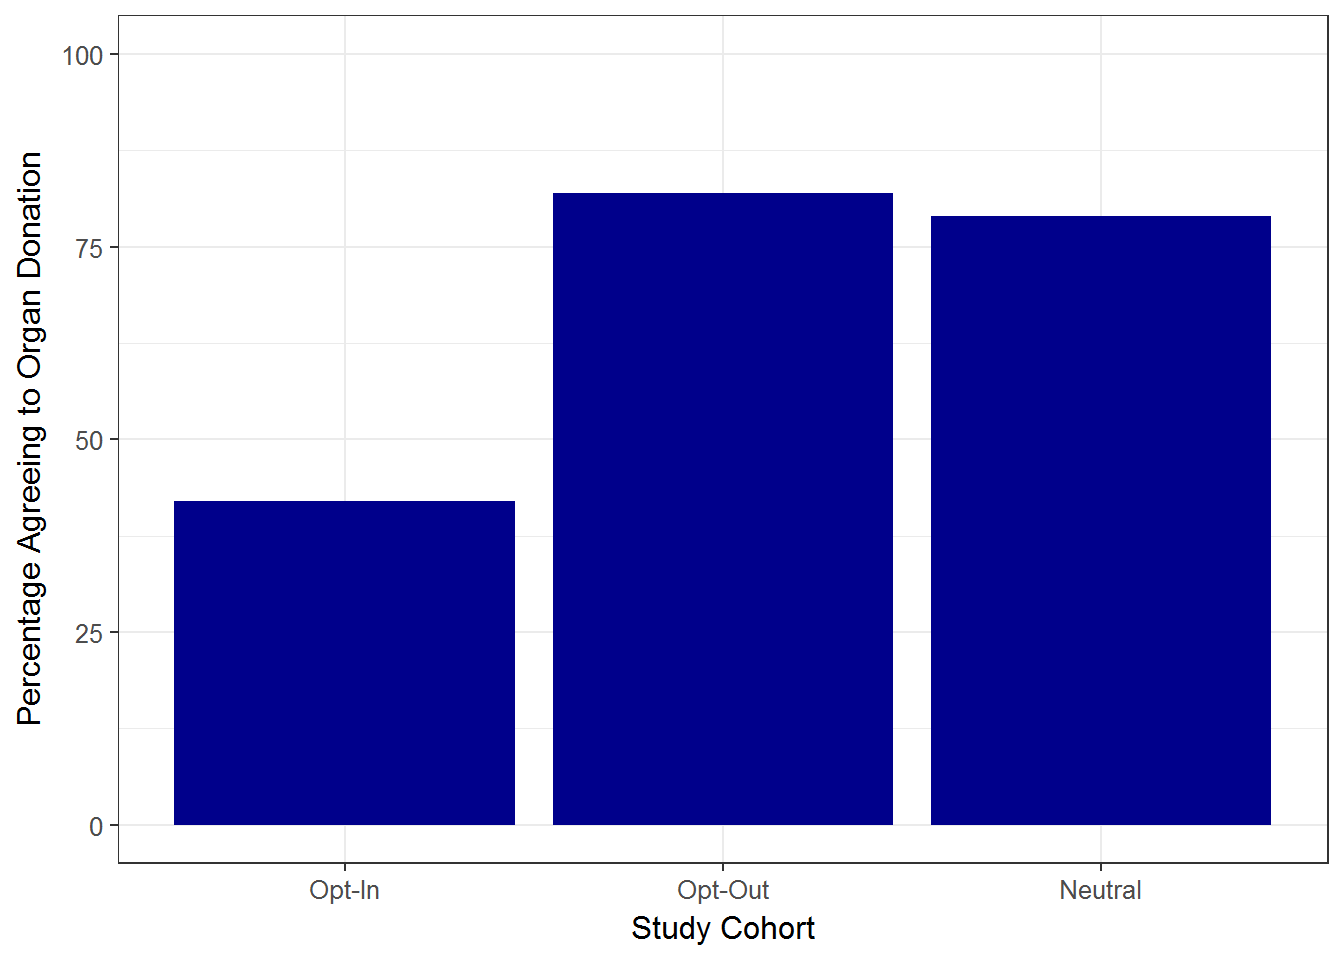
\includegraphics[width=0.8\linewidth]{./Images/basics-organ-plot-1} 

}

\caption{Summary of the responses for the Organ
Donation Study described in Example \ref{ex:basics-organ-donation}.}\label{fig:basics-organ-plot}
\end{figure}

\section{Overview of Drawing
Inference}\label{overview-of-drawing-inference}

Let's begin by taking a step back and considering the big picture of how
data is turned into information. Every research question we pose, at its
heart, is trying to characterize a \textbf{population}, the group of
subjects of ultimate interest.

\BeginKnitrBlock{definition}[Population]
\protect\hypertarget{def:defn-population}{}{\label{def:defn-population}
\iffalse (Population) \fi{} }The collection of subjects we would like to
say something about.
\EndKnitrBlock{definition}

In the Organ Donation study, the researchers would like to say something
about Americans who are of the age to consent to organ donation; in
particular, they would like to quantify how likely it is that someone
from this group agrees to organ donation. Therefore, the population is
the all Americans who are of the age to consent to organ donation. The
subjects in a population need not be people; the population could just
as easily be a collection of screws, sheet metal\ldots{}whatever
characterizes the objects from which we would \emph{like to} obtain
measurements. We use the phrase ``like to'' because in reality, it is
often impossible (or impractical) to observe the entire population.
Instead, we make observations on a subset of the population; this
smaller group is known as the \textbf{sample}.

\BeginKnitrBlock{definition}[Sample]
\protect\hypertarget{def:defn-sample}{}{\label{def:defn-sample}
\iffalse (Sample) \fi{} }The collection of subjects for which we
actually obtain measurements (data).
\EndKnitrBlock{definition}

For each subject within the sample, we obtain a collection of
measurements forming our set of data. The goal of statistical modeling
is to use the sample (the group we actually observe) to say something
about the population of interest (the group we wish we had observed);
this process is known as \textbf{statistical inference}. This process is
illustrated in Figure \ref{fig:basics-statistical-process}.

\BeginKnitrBlock{definition}[Statistical Inference]
\protect\hypertarget{def:defn-inference}{}{\label{def:defn-inference}
\iffalse (Statistical Inference) \fi{} }Sometimes referred to as
``inference,'' the process of using a sample to characterize some aspect
of the population.
\EndKnitrBlock{definition}

\begin{figure}

{\centering 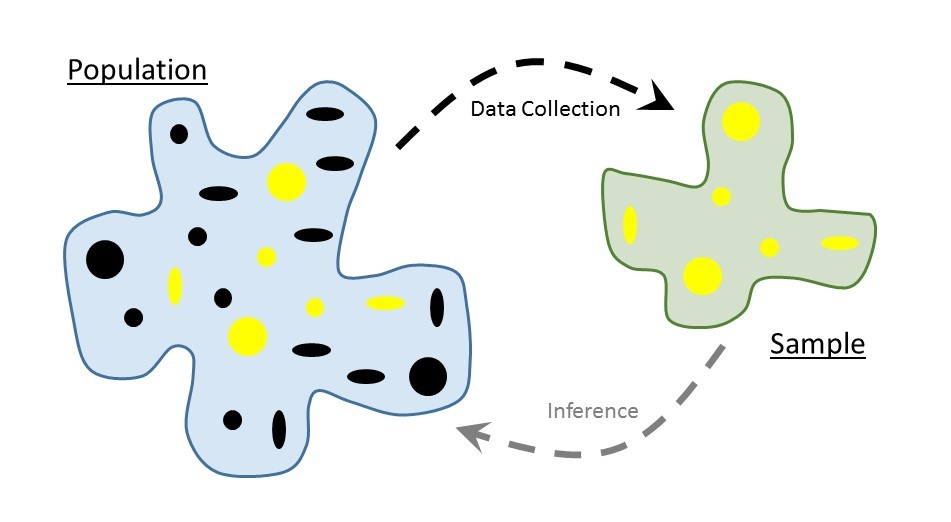
\includegraphics[width=0.8\linewidth]{images/Basics-Stat-Process} 

}

\caption{Illustration of the statistical process.}\label{fig:basics-statistical-process}
\end{figure}

\section{Anatomy of a Dataset}\label{anatomy-of-a-dataset}

Once we have our sample, we take measurements on each of the subjects.
These measurements form the data. When we hear the word ``data,'' most
of us envision a large spreadsheet. In reality, data can take on many
forms --- spreadsheets, images, text files, unstructured text from a
Twitter feed, etc. Regardless of the form, all datasets contain
information for each subject in the sample; this information, the
various measurements, are called \textbf{variables}.

\BeginKnitrBlock{definition}[Variable]
\protect\hypertarget{def:defn-variable}{}{\label{def:defn-variable}
\iffalse (Variable) \fi{} }A measurement, or category, describing some
aspect of the subject.
\EndKnitrBlock{definition}

Variables come in one of two flavors. \textbf{Categorical} variables are
those which denote a grouping to which the subject belongs. Examples
include marital status, brand, and experimental treatment group.
\textbf{Numeric} variables are those which take on values for which
ordinary arithmetic (addition, multiplication) makes sense. Examples
include height, age of a product, and diameter. Note that sometimes
numeric values are used to represent the levels of a categorical
variable in a dataset; for example, 0 may indicate ``No'' and 1 may
indicate ``Yes'' for a variable capturing whether a person is a
registered organ donor. Therefore, just because a variable has a numeric
value does not make it a numeric variable; the key here is that numeric
variables are those for which arithmetic makes sense.

\BeginKnitrBlock{definition}[Categorical Variable]
\protect\hypertarget{def:defn-categorical}{}{\label{def:defn-categorical}
\iffalse (Categorical Variable) \fi{} }Also called a ``qualitative
variable,'' a measurement on a subject which denotes a grouping or
categorization.
\EndKnitrBlock{definition}

\BeginKnitrBlock{definition}[Numeric Variable]
\protect\hypertarget{def:defn-numeric}{}{\label{def:defn-numeric}
\iffalse (Numeric Variable) \fi{} }Also called a ``quantitative
variable,'' a measurement on a subject which takes on a numeric value
\emph{and} for which ordinary arithmetic makes sense.
\EndKnitrBlock{definition}

While it may be natural to think of a dataset as a spreadsheet, not all
spreadsheets are created equal. Here, we consider datasets which have
the following characteristics:

\begin{itemize}
\tightlist
\item
  Each column contains a unique variable.
\item
  Each record (row in the dataset) corresponds to a different
  observation of the variables.
\item
  If you have multiple datasets, they should include a column in the
  table that allows them to be linked (subject identifier).
\end{itemize}

These are characteristics of ``tidy data.'' Even unstructured data such
as images or Twitter feeds must be processed, often converted to tidy
data, prior to performing a statistical analysis. The above description
eliminates a common method of storing data in engineering ans scientific
disciplines --- storing each sample in a different column. To
illustrate, suppose we conduct a study comparing the lifetime (in hours)
of two brands of batteries. We measure the lifetime of five batteries of
Brand A and six of Brand B. It is common to see a dataset like that in
Table \ref{tab:basics-poor-dataset}; the problem here is that the first
record of the dataset contains information on two different
observations. We have the lifetime from a battery of Brand A in the same
row as the lifetime from a battery of Brand B.

\begin{table}

\caption{\label{tab:basics-poor-dataset}Example of a common data structure which does not represent tidy data.  Data is from a hypothetical study comparing battery lifetimes (hours).}
\centering
\begin{tabular}[t]{l|l}
\hline
Brand A & Brand B\\
\hline
8.3 & 8.4\\
\hline
5.1 & 8.6\\
\hline
3.3 & 3.8\\
\hline
5.3 & 4.1\\
\hline
5.7 & 4.5\\
\hline
 & 4.0\\
\hline
\end{tabular}
\end{table}

In order to adhere to the tidy structure, we can reformat this dataset
as illustrated in Table \ref{tab:basics-good-dataset}. Here, each record
represents a unique observation and each column is a different variable.
We have also added a unique identifier.

\begin{table}

\caption{\label{tab:basics-good-dataset}Example of a tidy dataset, a good way of storing data.  Data is from a hypothetical study comparing battery lifetimes (hours).}
\centering
\begin{tabular}[t]{r|l|r}
\hline
Battery & Brand & Lifetime\\
\hline
1 & A & 8.3\\
\hline
2 & A & 5.1\\
\hline
3 & A & 3.3\\
\hline
4 & A & 5.3\\
\hline
5 & A & 5.7\\
\hline
6 & B & 8.4\\
\hline
7 & B & 8.6\\
\hline
8 & B & 3.8\\
\hline
9 & B & 4.1\\
\hline
10 & B & 4.5\\
\hline
11 & B & 4.0\\
\hline
\end{tabular}
\end{table}

It may take some time to get used to storing data in this format, but it
makes analysis easier and avoids time spent managing the data later.

\section{A Note on Codebooks}\label{a-note-on-codebooks}

A dataset on its own is meaningless if you cannot understand what the
values represent. \emph{Before} you access a dataset, you should always
review any available \textbf{codebooks}.

\BeginKnitrBlock{definition}[Codebook]
\protect\hypertarget{def:defn-codebook}{}{\label{def:defn-codebook}
\iffalse (Codebook) \fi{} }Also called a ``data dictionary,'' these
provide complete information regarding the variables contained within a
dataset.
\EndKnitrBlock{definition}

Some codebooks are excellent, with detailed descriptions of how the
variables were collected and appropriate units. Other codebooks are not
as good, giving only an indication of what the variable represents.
Whenever you are working with previously collected data, reviewing a
codebook is the first step; and, you should be prepared to revisit the
codebook often throughout an analysis. When you are collecting your own
dataset, constructing a codebook is essential for others to make use of
your data.

\hypertarget{CaseDeepwater}{\chapter{Case Study: Health Effects of the
Deepwater Horizon Oil Spill}\label{CaseDeepwater}}

On the evening of April 20, 2010, the \emph{Deepwater Horizon}, an oil
drilling platform positioned off the coast of Louisiana, was engulfed in
flames as the result of an explosion. The drilling rig, leased and
operated by BP, had been tasked with drilling an oil well in water
nearly 5000 feet deep. Eleven personnel were killed in the explosion.
The following clip is from the initial coverage by the \emph{New York
Times}\footnote{\url{http://www.nytimes.com/2010/04/22/us/22rig.html?rref=collection\%2Ftimestopic\%2FOil\%20Spills\&action=click\&contentCollection=timestopics\&region=stream\&module=stream_unit\&version=search\&contentPlacement=1\&pgtype=collection}}:




\begin{figure}

{\centering 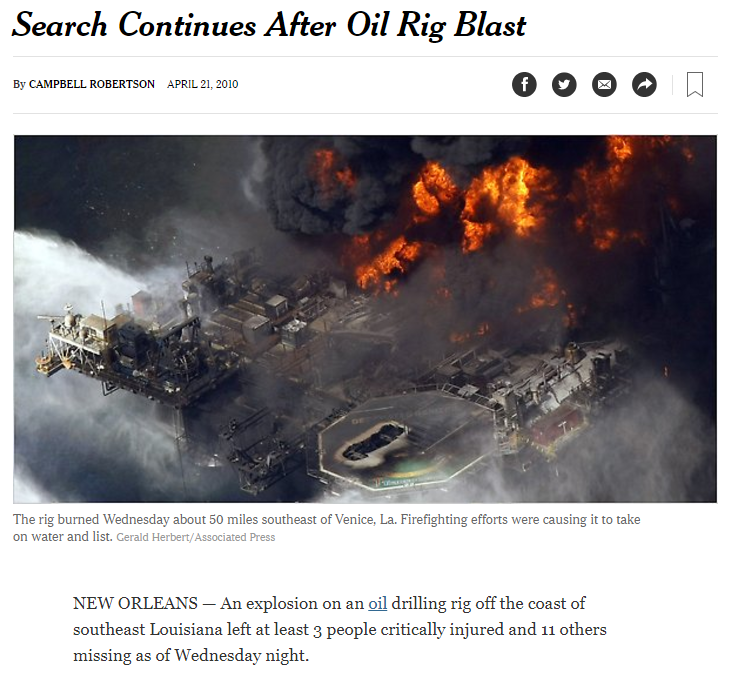
\includegraphics[width=0.8\linewidth]{./images/Case-Deepwater-NYTclip} 

}

\caption{\emph{New York Times} coverage of the
\emph{Deepwater Horizon} oil spill.}\label{fig:casedeepwater-nytclip}
\end{figure}

The incident is considered the worst oil spill in US history, creating
an environmental disaster along the Gulf Coast. In addition to studying
the effects on the local environment, researchers have undertaken
studies to examine the short and long-term health effects caused by the
incident. As an example, it is reasonable to ask whether volunteers who
were directly exposed to oil, such as when cleaning wildlife, are at
higher risk of respiratory irritation compared to those volunteers who
were helping with administrative tasks and therefore were not directly
exposed to the oil. An article appearing in \emph{The New England
Journal of Medicine} (B. D. Goldstein, Osofsky, and Lichtveld
\protect\hyperlink{ref-Goldstein2011}{2011}) reported the results from a
health symptom survey performed in the Spring and Summer of 2010 by the
National Institute for Occupational Safety and Health. Of 54 volunteers
assigned to wildlife cleaning and rehabilitation, 15 reported
experiencing ``nose irritation, sinus problems, or sore throat.'' Of 103
volunteers who had no exposure to oil, dispersants, cleaners, or other
chemicals, 16 reported experiencing ``nose irritation, sinus problems,
or sore throat.''

While a larger fraction of volunteers cleaning wildlife \emph{in the
study} reported respiratory symptoms compared to those who were not
directly exposed to irritants, would we expect similar results if we
were able to interview all volunteers? What about during a future oil
spill? Is there evidence that more than 1 in 5 volunteers who clean
wildlife will develop respiratory symptoms? What is a reasonable value
for the increased risk of respiratory symptoms for those volunteers with
direct exposure compared to those without?

In the first part of this text, we use this case study as the context
for discussing how research questions should be framed, methods for data
collection, summarizing and presenting data clearly, quantifying the
variability in an estimate, and quantifying the degree to which the data
disagrees with a proposed model. We capture these ideas in what we call
the \emph{Five Fundamental Ideas of Inference}. We see that any
statistical analysis iterates between the components of what we call the
\emph{Distributional Quartet}. These two frameworks allow us to describe
the language and logic of inference, serving as a foundation for the
statistical thinking and reasoning needed to address more complex
questions encountered later in the text.

\chapter{Asking the Right Questions}\label{Questions}

The discipline of statistics is about turning data into information in
order to address some question. While there may be no such thing as a
stupid question, there are ill-posed questions --- those which cannot be
answered as stated. Consider the
\protect\hyperlink{CaseDeepwater}{Deepwater Horizon Case Study}. It
might seem natural to ask ``if a volunteer cleans wildlife, will she
develop adverse respiratory symptoms?'' However, we quickly see that
this is an ill-posed question. Of the Of 54 volunteers assigned to
wildlife cleaning and rehabilitation, 15 reported experiencing adverse
respiratory symptoms (``nose irritation, sinus problems, or sore
throat''). So, while some volunteers developed symptoms, others did not.
What makes the question ill-posed is \emph{variability}, the fact that
not every volunteer had the same reaction when directly exposed to oil.

It is variability that creates a need for statistics; in fact, you could
think of statistics as the study and characterization of variability. We
must therefore learn to ask the \emph{right} questions --- those which
can be answered in the presence of variability.

\BeginKnitrBlock{definition}[Variability]
\protect\hypertarget{def:defn-variability}{}{\label{def:defn-variability}
\iffalse (Variability) \fi{} }The notion that measuremenets differ from
one observation to another.
\EndKnitrBlock{definition}

\BeginKnitrBlock{rmdkeyidea}
The presence of variability makes some questions ill-posed; statistics
concerns itself with how to address questions in the presence of
variability.
\EndKnitrBlock{rmdkeyidea}

\section{Characterizing a Variable}\label{characterizing-a-variable}

Recall that the goal of statistical inference is to say something about
the population; as a result, any question we ask should then be centered
on this larger group. The first step to constructing a well-posed
question is then to identify the population of interest for the study.
For the \protect\hyperlink{CaseDeepwater}{Deepwater Horizon Case Study},
it is unlikely that we are only interested in these 54 observed
volunteers assigned to wildlife cleaning. In reality, we might want to
say something about volunteers for any oil spill. In this case, the 54
volunteers in our dataset form the sample, a subset from all volunteers
who clean wildlife following an oil spill. That is, our population of
interest is comprised of all volunteers who clean wildlife following an
oil spill.

\BeginKnitrBlock{rmdtip}
When identifying the population of interest, be specific! Are you really
interested in \emph{all} trees, for example? Or, are you interested in
Maple trees within the city limits of Terre Haute, Indiana?
\EndKnitrBlock{rmdtip}

Since we expect that the reaction to oil exposure --- the primary
variable of interest for this study, sometimes called the
\textbf{response} --- to vary from one individual to another, we cannot
ask a question about the \emph{value} of the reaction (whether they
experienced symptoms or not). Instead, we want to characterize the
\textbf{distribution} of the response.

\BeginKnitrBlock{definition}[Response]
\protect\hypertarget{def:defn-response}{}{\label{def:defn-response}
\iffalse (Response) \fi{} }The primary variable of interest within a
study.
\EndKnitrBlock{definition}

\BeginKnitrBlock{definition}[Distribution]
\protect\hypertarget{def:defn-distribution}{}{\label{def:defn-distribution}
\iffalse (Distribution) \fi{} }The pattern of variability corresponding
to a set of values.
\EndKnitrBlock{definition}

Notice that in this case, the response is a categorical variable;
describing such a variable is equivalent to describing how individuals
in are divided among the possible groups. With a finite number of
observations, we could present the number of observations
(\textbf{frequeny}) within each group. For example, of the 54
volunteers, 15 experienced adverse symptoms and 39 did not. This works
well within the sample; however, as our population is infinitely large
(all volunteers cleaning wildlife on any oil spill), reporting the
frequencies is not appropriate. In this case, we report the fraction of
observations (\textbf{relative frequency}) falling within each group.

\BeginKnitrBlock{definition}[Frequency]
\protect\hypertarget{def:defn-frequency}{}{\label{def:defn-frequency}
\iffalse (Frequency) \fi{} }The number of observations falling into a
particular level of a categorical variable.
\EndKnitrBlock{definition}

\BeginKnitrBlock{definition}[Relative Frequency]
\protect\hypertarget{def:defn-relative-frequency}{}{\label{def:defn-relative-frequency}
\iffalse (Relative Frequency) \fi{} }Also called the ``proportion,'' the
fraction of observations falling into a particular level of a
categorical variable.
\EndKnitrBlock{definition}

Numeric quantities, like the proportion, which summarize the
distribution of a variable within the population are known as
\textbf{parameters}.

\BeginKnitrBlock{definition}[Parameter]
\protect\hypertarget{def:defn-parameter}{}{\label{def:defn-parameter}
\iffalse (Parameter) \fi{} }Numeric quantity which summarizes the
distribution of a variable within the \emph{population} of interest.
\EndKnitrBlock{definition}

While the \emph{value} of a variable may vary across the population, the
\emph{parameter} is a single fixed constant which summarizes the
variable for that population. Therefore, well-posed questions can be
constructed if we limit ourselves to questions about the parameter. The
second step in constructing well-posed questions is then to identify the
parameter of interest.

The questions we ask then generally fall into one of two categories:

\begin{itemize}
\tightlist
\item
  Estimation: what \emph{proportion} of volunteers who clean wildlife
  following an oil spill will experience adverse respiratory symptoms?
\item
  Model Consistency: is it reasonable that no more than 1 in 5
  volunteers who clean wildlife following an oil spill will experience
  adverse respiratory symptoms?
\end{itemize}

Now, since we do not get to observe the population (we only see the
sample), we cannot observe the value of the parameter. That is, we will
never know the true proportion of volunteers who will experience
symptoms. However, we can determine what the data suggests about the
population (that's inference).

\BeginKnitrBlock{definition}[Estimation]
\protect\hypertarget{def:defn-estimation}{}{\label{def:defn-estimation}
\iffalse (Estimation) \fi{} }Using the sample to approximate the value
of a parameter from the underlying population.
\EndKnitrBlock{definition}

\BeginKnitrBlock{definition}[Hypothesis Testing]
\protect\hypertarget{def:defn-hypothesis-testing}{}{\label{def:defn-hypothesis-testing}
\iffalse (Hypothesis Testing) \fi{} }Using a sample to determine if the
data is consistent with a working theory or if there is evidence to
suggest the data is not consistent with the theory.
\EndKnitrBlock{definition}

\BeginKnitrBlock{rmdkeyidea}
Parameters are unknown values and can, in general, never be known.
Parameters are generally denoted by Greek letters in statistical
formulas.
\EndKnitrBlock{rmdkeyidea}

It turns out, the vast majority of research questions can be framed in
terms of a parameter. In fact, this is the first of what we consider the
\emph{Five Fundamental Ideas of Inference}.

\BeginKnitrBlock{rmdfivefund}
\textbf{Fundamental Idea I}: A research question can often be framed in
terms of a parameter which characterizes the population. Framing the
question should then guide our analysis.
\EndKnitrBlock{rmdfivefund}

\section{Framing the Question}\label{framing-the-question}

In engineering and scientific applications, many questions fall under
the second category of model consistency. Examining such questions is
known as \textbf{hypothesis testing}. Specifically, data is collected to
help the researcher choose between two competing theories for the
parameter of interest. In this section, we consider the terminology
surrounding specifying such questions.

For the \protect\hyperlink{CaseDeepwater}{Deepwater Horizon Case Study}
suppose we are interested in addressing the following question:

\begin{quote}
Is there evidence that more than 1 in 5 volunteers who clean wildlife
following an oil spill will develop adverse respiratory symptoms?
\end{quote}

The question itself is about the population (all volunteers assigned to
clean wildlife following an oil spill) and is centered on a parameter
(the proportion who develop adverse respiratory symptoms). That is, this
is a well-posed question that can be answered with appropriate data. The
overall process for addressing these types of questions is similar to
conducting a trial in a court of law. In the United States, a trial has
the following essential steps:

\begin{enumerate}
\def\labelenumi{\arabic{enumi}.}
\tightlist
\item
  Assume the defendant is innocent.
\item
  Evidence to establish guilt (to the contrary of innocence) is
  presented by the prosecution.
\item
  The jury considers the weight of the evidence.
\item
  If the evidence is ``beyond a reasonable doubt,'' the jury declares
  the defendant guilty; otherwise, the jury declares the subject not
  guilty.
\end{enumerate}

The process of conducting a hypothesis test has similar essential steps:

\begin{enumerate}
\def\labelenumi{\arabic{enumi}.}
\tightlist
\item
  Assume the innocent of what we want the data to show (develop a
  working theory).
\item
  Gather data and compare it to the proposed model.
\item
  Quantify the likelihood of our data under the proposed model.
\item
  If the likelihood is small, conclude the data is not consistent with
  the working model (there is evidence for what we want to show);
  otherwise, conclude the data is consistent with the working model
  (there is no evidence for what we want to show).
\end{enumerate}

Notice that a trial focuses not on proving guilt but on disproving
innocence; similarly, in statistics, we are able to establish evidence
\emph{against} a specified theory. This process has several subtle
points including this one. We will discuss these subtleties at various
points throughout the text and revisit the overall concepts often. Here,
we focus solely on that first step --- developing a working theory that
we want to \emph{disprove}.

Consider the above question for the
\protect\hyperlink{CaseDeepwater}{Deepwater Horizon Case Study}. We want
to find evidence that the proportion experiencing adverse symptoms
exceeds 0.20 (1 in 5). Therefore, we would like to \emph{disprove} (or
provide evidence \emph{against}) the statement that the proportion
experiencing adverse symptoms is no more than 0.20. This is known as the
\textbf{null hypothesis}; the opposite of this statement, called the
\textbf{alternative hypothesis}, captures what we would like to
establish.

\BeginKnitrBlock{definition}[Null Hypothesis]
\protect\hypertarget{def:defn-null-hypothesis}{}{\label{def:defn-null-hypothesis}
\iffalse (Null Hypothesis) \fi{} }The statement (or theory) that we
would like to \emph{disprove}. This is denoted \(H_0\), read
``H-naught'' or ``H-zero''.
\EndKnitrBlock{definition}

\BeginKnitrBlock{definition}[Alternative Hypothesis]
\protect\hypertarget{def:defn-alternative-hypothesis}{}{\label{def:defn-alternative-hypothesis}
\iffalse (Alternative Hypothesis) \fi{} }The statement (or theory)
capturing what we would like to provide evidence \emph{for}; this is the
opposite of the null hypothesis. This is denoted \(H_1\) or \(H_a\),
read ``H-one'' and ``H-A'' respectively.
\EndKnitrBlock{definition}

For the \protect\hyperlink{CaseDeepwater}{Deepwater Horizon Case Study},
we write:

\begin{quote}
\(H_0:\) The proportion of volunteers assigned to wildlife following an
oil spill who experience adverse respiratory symptoms is no more than
0.20.\\
\(H_1:\) The proportion of volunteers assigned to wildlife following an
oil spill who experience adverse respiratory symptoms exceeds 0.20.
\end{quote}

Each hypothesis is a well-posed statement (about a parameter
characterizing the entire population), and the two statements are
exactly opposite of one another meaning only one can be a true
statement. We can now collect data to determine if it is consistent with
the null hypothesis (a statement similar to ``not guilty'') or if the
data provides evidence against the null hypothesis and in favor of the
alternative (a statement similar to ``guilty'').

Often these statements are written in a bit more of a mathematical
structure in which a Greek letter is used to represent the parameter of
interest. For example, we might write

\begin{quote}
Let \(\theta\) be the proportion of volunteers (assigned to wildlife
following an oil spill) who experience adverse respiratory symptoms.\\
\(H_0: \theta \leq 0.20\)\\
\(H_1: \theta > 0.20\)
\end{quote}

In the above statements, \(\theta\) represents the parameter of
interest; the value 0.20 is known as the \textbf{null value}.

\BeginKnitrBlock{definition}[Null Value]
\protect\hypertarget{def:defn-null-value}{}{\label{def:defn-null-value}
\iffalse (Null Value) \fi{} }The value associated with the equality
component of the null hypothesis; it forms the threshold or boundary
between the two hypothesis. Note: not all questions of interest require
a null value be specified.
\EndKnitrBlock{definition}

\BeginKnitrBlock{rmdkeyidea}
Hypothesis testing is a form of statistical inference in which we
quantify the evidence \emph{against} a working theory (captured by the
null hypothesis). We essentially argue that the data supports the
alternative if it is not consistent with the working theory.
\EndKnitrBlock{rmdkeyidea}

\BeginKnitrBlock{rmdtip}
\textbf{Process for Framing a Question} In order to frame a research
question, consider the following steps:

\begin{enumerate}
\def\labelenumi{\arabic{enumi}.}
\tightlist
\item
  Identify the population of interest.
\item
  Identify the parameter(s) of interest.
\item
  Determine if you are interested in estimating the parameter(s) or
  quantifying the evidence against some working theory.
\item
  If you are interested in testing a working theory, make the null
  hypothesis the working theory and the alternative the exact opposite
  statement (what you want to provide evidence for).
\end{enumerate}
\EndKnitrBlock{rmdtip}

\chapter{Gathering the Evidence (Data Collection)}\label{Data}

Consider again the goal of statistical inference --- to use a sample as
a snapshot to say something about the underlying population (Figure
\ref{fig:data-statistical-process}). This generally provokes unease in
people, leading to a distrust of statistical results. In this section we
attack that distrust head on.

\begin{figure}

{\centering 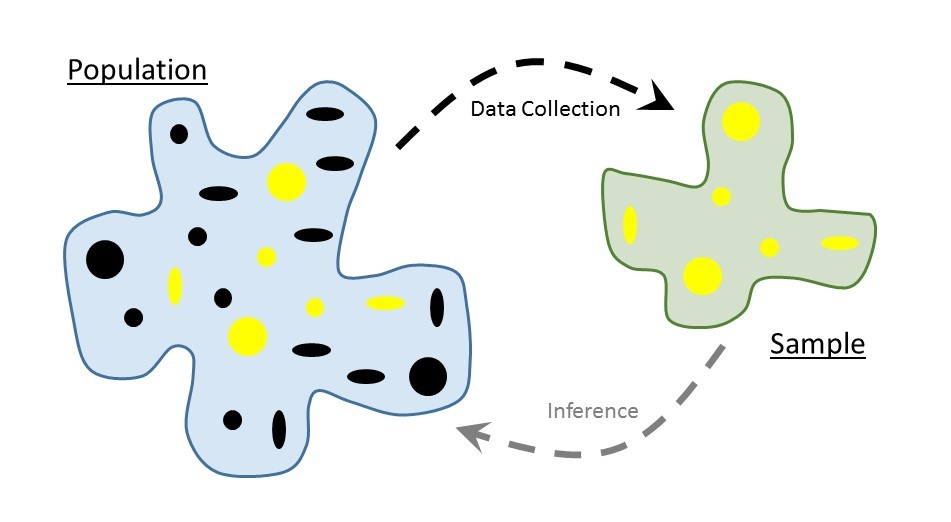
\includegraphics[width=0.8\linewidth]{images/Basics-Stat-Process} 

}

\caption{Illustration of the statistical process (reprinted from Chapter 1).}\label{fig:data-statistical-process}
\end{figure}

\section{What Makes a Sample
Reliable}\label{what-makes-a-sample-reliable}

If we are going to have some amount of faith in the statistical results
we produce, we must have data in which we can place our trust. \emph{The
Treachery of Images} (Figure @\ref(fig:data-pipe-img)) is a canvas
painting depicting a pipe, below which the artist wrote the French
phrase for ``This is not a pipe.'' Regarding the painting, the artist
said

\begin{quote}
The famous pipe. How people reproached me for it! And yet, could you
stuff my pipe? No, it's just a representation, is it not? So if I had
written on my picture ``This is a pipe,'' I'd have been lying!
\end{quote}




\begin{figure}

{\centering 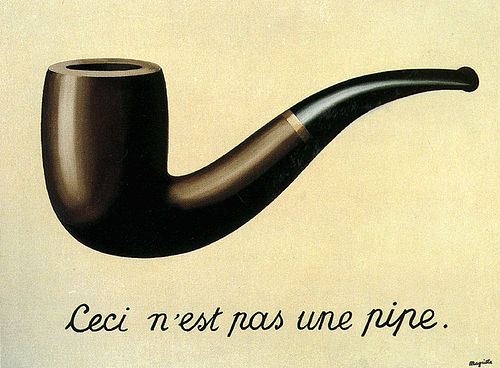
\includegraphics[width=0.8\linewidth]{./images/Data-Pipe} 

}

\caption{\emph{The Treachery of Images} by René
Magritte.}\label{fig:data-pipe-img}
\end{figure}

Just as a painting is a representation of the object it depicts, so a
sample should be a representation of the underlying population from
which it was taken. This is the primary requirement if we are to rely on
the resulting data.

\BeginKnitrBlock{rmdkeyidea}
In order for a statistical analysis to be reliable, the sample must be
\emph{representative} of the underlying population.
\EndKnitrBlock{rmdkeyidea}

We need to be careful to not get carried away in our expectations. What
constitutes ``representative'' really depends on the question, just as
an artist chooses his depiction based on how he wants to represent the
object. Let's consider the following example.

\BeginKnitrBlock{example}[School Debt]
\protect\hypertarget{exm:data-school-debt}{}{\label{exm:data-school-debt}
\iffalse (School Debt) \fi{} }In addition to a degree, college graduates
also tend to leave with a large amount of debt due to college loans. In
2012, a graduate with a student loan had an average debt of \$29,400;
for graduates from private non-profit institutions, the average debt was
\$32,300\footnote{\url{http://ticas.org/sites/default/files/pub_files/Debt_Facts_and_Sources.pdf}}.

Suppose we are interested in determining the average amount of debt in
student loans carried by a graduating senior from Rose-Hulman Institute
of Technology, a small private non-profit engineering school. There are
many faculty at Rose-Hulman who choose to send their children to the
institute. Since I am also on the faculty, I know many of these
individuals. Suppose I were to ask each to report the amount of student
loans their children carried upon graduation from Rose-Hulman. I compile
the 25 responses and compute the average amount of debt. Further, I
report that based on this study, there is significant evidence that the
average debt carried by a graduate of Rose-Hulman is far below the
\$32,300 reported above (great news for this year's graduating class)!
Why might we be hesitant to trust these results?
\EndKnitrBlock{example}

When our distrust of a statistical result stems from a distrust of the
data on which it is based, it is generally a result of our doubting the
sample is representative of the population. Rose-Hulman, like many other
universities, has a policy that the children of faculty may attend their
university (assuming admittance) tuition-free. We would therefore expect
their children to carry much less debt than the typical graduating
senior.

This provides a nice backdrop for discussing what it means to be
representative. First, let's define our population; in this case, we are
interested in graduating seniors. The variable of interest is the amount
of debt carried in student loans; the parameter of interest is then the
average amount of debt in student loans carried by graduating seniors.
With regard to the grade point average of the students in our sample, it
is probably similar to all graduating seniors. Their starting salary is
probably similar; the fraction of mechanical engineering majors versus
math majors is probably similar. So, in many regards the sample is
representative of the population; however, it fails to be representative
with regard to the variable of interest. This is our concern. The amount
of debt carried by students in our sample is not representative of that
debt carried by all graduating seniors.

\BeginKnitrBlock{rmdtip}
When thinking about whether a sample is representative, focus your
attention to the characteristics specific to your research question.
\EndKnitrBlock{rmdtip}

Does that mean the sample is useless? Yes and no. The sample collected
cannot be used to answer our initial question of interest. No
statistical method can fix bad data; statistics adheres to the
``garbage-in, garbage-out'' phenomena. If the data is bad, no analysis
will undo that. While the sample cannot be used to answer our initial
question, it could be used to address a different question however:

\begin{quote}
What is the average amount of debt in student loans carried by
graduating seniors from Rose-Hulman whose parent is a faculty member at
the university?
\end{quote}

For this revised question, the sample may indeed be representative. If
we are working with previously collected data, we must consider the
population to which our results will generalize. That is, for what
population is the given sample representative. If we are collecting our
data, we need to be sure we collect data in such a way that the data is
representative. Let's first look at what \emph{not} to do.

\section{Poor Methods of Data
Collection}\label{poor-methods-of-data-collection}

Example \ref{ex:data-school-debt} is an example of a ``convenience
sample,'' when the subjects in the sample are chosen simply due to ease
of collection. Examples include surveying students only in your sorority
when you are interested in all females who are part of a sorority on
campus; taking soil samples from only your city when you are interested
in the soil for the entire state; and, obtaining measurements from only
one brand of phone, because it was the only one you could afford on your
budget, when you are interested in studying all cell phones on the
market. A convenience sample is unlikely to be representative if there
is a relationship between the ease of collection and the variable under
study. This was true in the School Debt example; the relationship of a
student to a faculty member was directly related to the amount of debt
they carried. As a result, the resulting sample was not representative
of the population.

When conducting a survey with human subjects, it is common to only
illicit responses from volunteers. Such ``volunteer samples'' tend to
draw in those with extreme opinions. Consider product ratings on Amazon.
Individual ratings tend to cluster around 5's and 1's. This is because
those customers who take time to submit a review (which is voluntary)
tend to be those who are really thrilled with their product (and want to
encourage others to purchase it) and those who are really disappointed
with their purchase (and want to encourage others to avoid it). Such
surveys often fail to capture those individuals in the population who
have intermediate opinions.

We could not possibly name all the poor methods for collecting a sample;
but, these methods all share something in common --- it is much more
likely the resulting sample is not representative. Failing to be
representative results in \textbf{biased} estimates of the parameter.

\BeginKnitrBlock{definition}[Bias]
\protect\hypertarget{def:defn-bias}{}{\label{def:defn-bias} \iffalse (Bias)
\fi{} }A set of measurements, or an estimate of a parameter, is said to
be biased if they are \emph{consistently} too high (or too low).
\EndKnitrBlock{definition}

To illustrate the concept of bias, consider shooting at a target as in
Figure \ref{fig:data-bias}. We can consider the center of our target to
be the parameter we would like to estimate within the population. The
values in our sample (the strikes on the target) will vary around the
parameter; while we do not expect any one value to hit the target
precisely, a ``representative'' sample is one in which the values tend
to be clustered about the parameter (unbiased). When the sample is not
representative, the values in the sample tend to cluster off the mark
(biased). Notice that to be unbiased, it may be that not a single value
in the sample is perfect, but aggregated together, they point in the
right direction. So, bias is not about an individual measurement being
an ``outlier,'' (more on those in a later chapter) but about repeatedly
shooting in the wrong direction.

\begin{figure}

{\centering 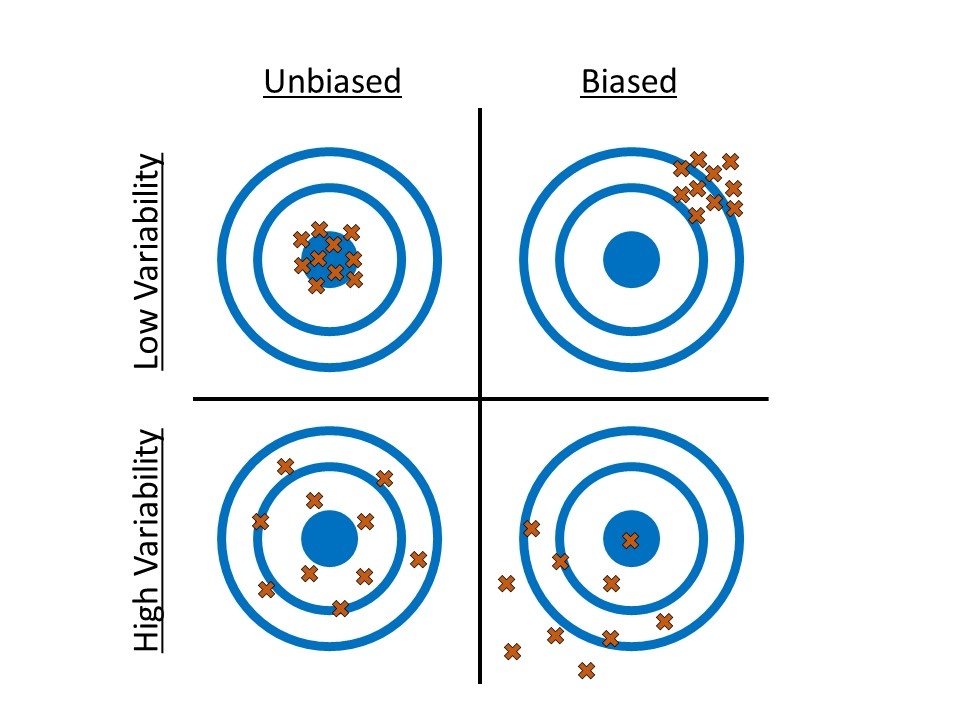
\includegraphics[width=0.8\linewidth]{./images/Data-Bias} 

}

\caption{Illustration of bias and variability.}\label{fig:data-bias}
\end{figure}

\BeginKnitrBlock{rmdkeyidea}
Biased results are typically due to poor sampling methods that result in
a sample which is not representative of the underlying population.
\EndKnitrBlock{rmdkeyidea}

The catch (there is always a catch) is that we will never know if a
sample is representative or not. But, we can employ methods that help to
minimize the chance that the sample is biased.

\section{Preferred Methods of
Sampling}\label{preferred-methods-of-sampling}

No method guarantees a perfectly representative sample; but, we can take
measures to reduce or eliminate bias. A useful strategy is to employ
\emph{randomization}. This is summarized in our second Fundamental Idea:

\BeginKnitrBlock{rmdfivefund}
\textbf{Fundamental Idea II}: If data is to be useful for making
conclusions about the population, a process referred to as drawing
inference, proper data collection is crucial. Randomization can play an
important role ensuring a sample is representative and that inferential
conclusions are appropriate.
\EndKnitrBlock{rmdfivefund}

Consider the School Debt example again. Suppose instead of the strategy
described there, we had constructed a list of all graduating seniors
from the university. We placed the name of each student on an index
card; then, I thoroughly shuffle the cards and choose the top 25 cards.
For these 25 individuals, I record the amount of debt in student loans
each carries. Using a lottery to select the sample is known as a
\textbf{simple random sample}. By conducting a lottery, we make it very
unlikely that our sample consists of only students with a very small
amount of student debt (as occurred when we used a convenience sample).

\BeginKnitrBlock{definition}[Simple Random Sample]
\protect\hypertarget{def:defn-simple-random-sample}{}{\label{def:defn-simple-random-sample}
\iffalse (Simple Random Sample) \fi{} }Often abbreviated SRS, this is a
sample of size \(n\) such that \emph{every} collection of size \(n\) is
equally likely to be the resulting sample. This is equivalent to a
lottery.
\EndKnitrBlock{definition}

There are situations in which a simple random sample does not suffice.
Again, consider our School Debt example. The Rose-Hulman student body is
predominantly domestic, with only about 3\% of the student body being
international students. But, suppose we are interested in comparing the
average debt carried between international and domestic students. It is
very likely that in a simple random sample of 25 students, none will be
international by chance alone. Instead of a simple random sample, we
might consider taking a sample of, say 13, domestic students and a
sample of 12 international students; this is an example of a
\textbf{stratified random sample}. This approach is useful when there is
a natural grouping of interest within the population.

\BeginKnitrBlock{definition}[Stratified Random Sample]
\protect\hypertarget{def:defn-stratified-random-sample}{}{\label{def:defn-stratified-random-sample}
\iffalse (Stratified Random Sample) \fi{} }A sample in which the
population is first divided into groups, or strata, based on a
characteristic of interest; a simple random sample is then taken within
each group.
\EndKnitrBlock{definition}

There are countless sampling techniques used in practice. The two
described above can be very useful starting point for developing a
custom method suitable for a particular application. Their benefit stems
from their use of randomization.

This section is entitled ``Preferred Methods'' because while these
methods are ideal, they are not always practical. For example, consider
the \protect\hyperlink{CaseDeepwater}{Deepwater Horizon Case Study};
conceptually, we can take a simple random sample of the volunteers for
our study. However, as with any study involving human subjects,
researchers would be required to obtain consent from each subject in the
study. That is, a volunteer has the right to refuse to participate in
the study. Therefore, it is unlikely that a simple random sample as
described above could be obtained. Again, the key is to obtain a
\emph{representative} sample; while random selection may be a nice tool
for accomplishing this, we may need to appeal to the composition of the
sample itself to justify its use. Based on the characteristics of those
willing to participate in the study, do we feel the study participants
form a representative group of all volunteers? That is the essential
question. This is often why studies report a table summarizing subject
demographics such as age, gender, etc. It is also why it is extremely
important for researchers to describe how subjects were selected so that
readers may make the judgement for themselves whether the sample is
representative.

\section{Two Types of Studies}\label{two-types-of-studies}

Thinking about how the data was collected helps us determine how the
results generalize beyond the sample itself (to what population the
results apply). When our question of interest is about the relationship
between two variables (as most questions are), we must also carefully
consider the study design. Too often separated from the statistical
analysis that follows, keeping the study design in mind should guide the
analysis as well as inform us about the conclusions we can draw.

In order to illustrate how study design can impact the results, consider
the following example.

\BeginKnitrBlock{example}[Kangaroo Care]
\protect\hypertarget{exm:data-kangaroo}{}{\label{exm:data-kangaroo}
\iffalse (Kangaroo Care) \fi{} }At birth, infants have low levels of
Vitamin K, a vitamin needed in order to form blood clots. Though rare,
without the ability for her blood to clot, an infant could develop a
serious bleed. In order to prevent this, the American Academy of
Pediatrics recommends that all infants be given a Vitamin K shot shortly
after birth in order to raise Vitamin K levels. As with any shot, there
is typically discomfort to the infant, which can be very discomforting
to new parents.

Kangaroo Care is a method of holding a baby which emphasizes
skin-to-skin contact. The child, who is dressed only in a diaper, is
placed upright on the parent's bare chest; a light blanket is draped
over the child. The method was initially recognized for its benefits in
caring for pre-term infants. Suppose suppose we are interested in
determining if utilizing the method while giving the child a Vitamin K
shot reduces the discomfort in the infant, as measured by the total
amount of time the child cries following the shot. Contrast the
following two potential study designs:

\begin{enumerate}
\def\labelenumi{(\Alph{enumi})}
\tightlist
\item
  We allow the attending nurse to determine whether Kangaroo Care is
  initiated prior to giving the Vitamin K shot. Following the shot, we
  record the total time (in seconds) the child cries.
\item
  We flip a coin. If it comes up heads, the nurse should have the
  parents implement Kangaroo Care prior to giving the Vitamin K shot; if
  it comes up tails, the nurse should give the Vitamin K shot without
  implementing Kagaroo Care. Following the shot, we record the total
  time (in seconds) the child cries.
\end{enumerate}

Note, in both study designs (A) and (B), we only consider term births
which have no complications to avoid potential complications that might
alter the timing of the Vitamin K shot or the ability to implement
Kangaroo Care.
\EndKnitrBlock{example}

Note that there are some similarities in the two study designs:

\begin{itemize}
\tightlist
\item
  The underlying population is the same for both designs --- infants
  born at term with no complications.
\item
  There are two treatment groups in both designs --- the ``Kangaroo
  Care'' group and the ``no Kangaroo Care'' group.
\item
  The response (variable of interest) is the same in both designs ---
  the time (in seconds) the infant cries.
\item
  There is action taken by the researcher in both designs --- a Vitamin
  K shot is given to the child.
\end{itemize}

There is one prominent difference between the two study designs:

\begin{itemize}
\tightlist
\item
  For design (A), the choice of Kangaroo Care is left up to the nurse
  (self-selected); for design (B), the choice of Kangaroo is
  \emph{assigned} to the nurse by the researcher, and this selection is
  made \emph{at random}.
\end{itemize}

Design (A) is an example of an \textbf{observational study}; design (B)
is a \textbf{controlled experiment}.

\BeginKnitrBlock{definition}[Observational Study]
\protect\hypertarget{def:defn-observational-study}{}{\label{def:defn-observational-study}
\iffalse (Observational Study) \fi{} }A study in which the subjects
self-select into the treatment groups under study.
\EndKnitrBlock{definition}

\BeginKnitrBlock{definition}[Controlled Experiment]
\protect\hypertarget{def:defn-controlled-experiment}{}{\label{def:defn-controlled-experiment}
\iffalse (Controlled Experiment) \fi{} }A study in which the subjects
are \emph{randomly} assigned to the treatment groups under study.
\EndKnitrBlock{definition}

It is common to think that anytime the environment is ``controlled'' by
the researcher that an experiment is taking place, but the defining
characteristic is the random assignment to treatment groups (sometimes
referred to as the \emph{factor} under study). In the example above,
both study designs involved a controlled setting (the delivery room of a
hospital) in which trained staff (the nurse) delivered the shot.
However, only design (B) is a controlled experiment because the
researchers randomly determined into which group the infant would be
placed.

To understand the impact of random allocation, suppose that we had
conducted a study as in design (A); further, the results suggest that
those infants who were given a shot while using Kangaroo Care cried for
a shorter time period, on average. Can we conclude that it was the
Kangaroo Care that led to the shorter crying time? Maybe. Consider the
following two potential explanations for the resulting data:

\begin{enumerate}
\def\labelenumi{(\arabic{enumi})}
\tightlist
\item
  Kangaroo Care is very effective; as a result, those children who were
  given Kangaroo Care had reduced crying time following the Vitamin K
  shot.
\item
  It turns out that those nurses who chose to implement Kangaroo Care
  (remember, they have a choice under design (A) whether they implement
  the method) were also the nurses with a gentler bedside manner.
  Therefore, these nurses tended to be very gentle when giving the
  Vitamin K shot whereas the nurses who chose not to implement Kangaroo
  Care tended to just jab the needle in when giving the shot. As a
  result, the reduced crying time is not a result of the Kangaroo Care
  but the manner in which the shot was given.
\end{enumerate}

The problem is that we are unable to determine which of the explanations
is true. Given the data we have collected, we are unable to tease out
the effect of the Kangaroo Care from that of the nurse's bedside manner.
As a result, we are able to say we observed a \emph{relationship}
between the use of Kangaroo Care and reduced crying time, but we are
unable to conclude that Kangaroo Care \emph{caused} a reduction in the
crying time. In this hypothetical scenario, the nurse's bedside manner
is called a \textbf{confounder}.

\BeginKnitrBlock{definition}[Confounding]
\protect\hypertarget{def:defn-confounding}{}{\label{def:defn-confounding}
\iffalse (Confounding) \fi{} }When the effect of a variable on the
response is mis-represented due to the presence of a third, potentially
unobserved, variable known as a confounder.
\EndKnitrBlock{definition}

Confounders can mask the relationship between the factor under study and
the response. There is a documented relationship between ice cream sales
and the risk of shark attacks. As ice cream sales increase, the risk of
a shark attack also increases. This does not mean that if a small city
in the Midwest increases its ice cream sales that the citizens are at
higher risk of being attacked by a shark. As Figure
\ref{fig:data-confounding} illustrates, there is a confounder ---
temperature. As the temperatures increase, people tend to buy more ice
cream; as the temperature increases, people tend to go to the beach
increasing the risk of a shark attack. Two variables can appear to be
related as a result of a confounder.

\begin{figure}

{\centering 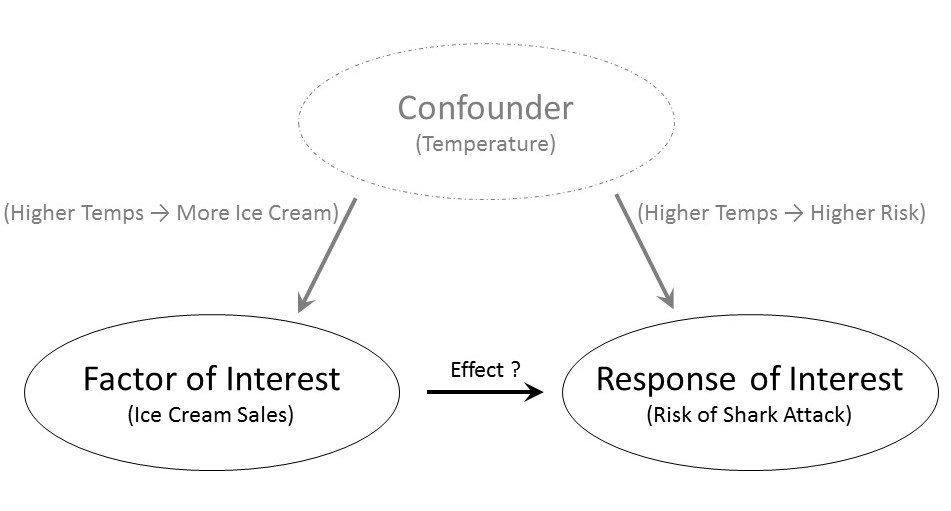
\includegraphics[width=0.8\linewidth]{./images/Data-Confounding} 

}

\caption{Illustration of a confounding variable. The confounder, related to both the factor and the treatment can make it appear as though there is a causal relationship when none exists.}\label{fig:data-confounding}
\end{figure}

\BeginKnitrBlock{rmdtip}
Confounders are variables that influence \emph{both} the factor of
interest and the response.
\EndKnitrBlock{rmdtip}

Observational studies are subject to confounding; thus, controlled
experiments are often considered the gold standard in research because
they allow us to infer cause-and-effect relationships from the data. Why
does the random allocation make such an impact? Because it removes the
impact of confounders. Let's return to the hypothetical study. Suppose
there are nurses with a gentle bedside manner and those who are a little
less gentle. If the infants are randomly assigned to one of the two
treatment groups, then for every gentle nurse who is told to implement
Kangaroo Care while giving the shot, there is a gentle nurse who is told
to not implement Kangaroo Care. Similarly, for every mean nurse who is
told to implement Kangaroo Care while giving a shot, there is a mean
nurse who is told to not implement Kangaroo Care. This is illustrated in
Figure \ref{fig:data-randomization}. For an observational study, the
treatment groups are unbalanced; there is a higher fraction (11/12
compared to 1/4) of friendly nurses in the Kangaroo Care group compared
to the No Kangaroo Care group. For the controlled experiment however,
the treatment groups are balanced; there is approximately the same
fraction of friendly nurses in both groups. Random assignment is the
great equalizer; it tends to result in groups which are similar in all
respects; therefore, any differences we observe between the groups
\emph{must} be due to the grouping and not an underlying confounding
variable.

\begin{figure}

{\centering 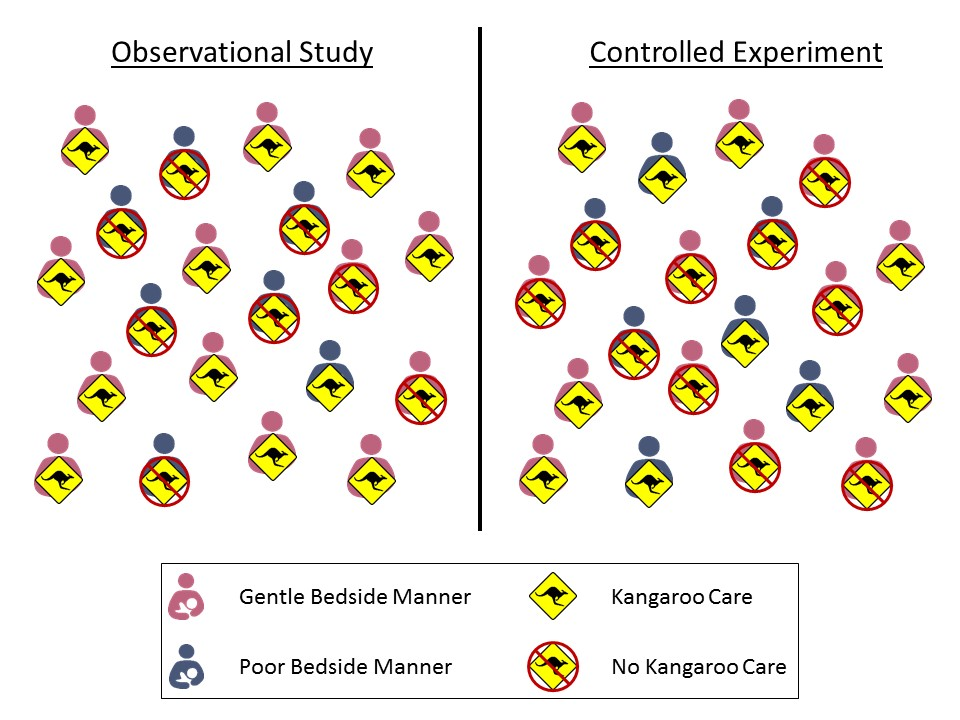
\includegraphics[width=0.8\linewidth]{./images/Data-Randomization} 

}

\caption{Illustration of the impact of random assignment in study design. For the observational study, the treatment groups are unbalanced.  For the controlled experiment, the treatment groups are balanced.}\label{fig:data-randomization}
\end{figure}

\BeginKnitrBlock{rmdkeyidea}
Randomly assigning treatment groups balances the groups with respect to
the confounders; that is, the treatment groups are similar. Therefore,
any differences between the two groups can be attributed to the grouping
factor itself.
\EndKnitrBlock{rmdkeyidea}

While controlled experiments are a fantastic study design, we should not
discount the use of observational studies. Consider the
\protect\hyperlink{CaseDeepwater}{Deepwater Horizon Case Study}; suppose
we are interested in the following question:

\begin{quote}
Is there evidence that volunteers who are directly exposed to oil have
an increased risk of developing adverse respiratory symptoms compared to
those who are not directly exposed to oil?
\end{quote}

The response is whether a volunteer develops adverse respiratory
symptoms; the factor of interest is whether the volunteer has direct
exposure to oil. We could conduct a controlled experiment by randomly
determining which volunteers are assigned to wildlife clean up and which
are assigned to administrative tasks, for example. However, it may be
that volunteer tasks need to be determined by skillset or by greatest
need at the time of the person volunteers. It may not be feasible to
randomly assign volunteers to specific positions. Or, it could be that
the data was obtained after the fact; that is, the data is not the
result of a planned study in which case random assignment is not
possible because volunteers self-selected into positions in the past. If
random assignment is not possible, it does not mean the data is useless.
But, it does mean we will need to be sure we address the potential
confounding when performing the analysis and discussing the results. The
latter half of the text will discuss methods for addressing confounding.

The big idea is that in order to make causal conclusions, we must be
able to state that the two treatment groups are balanced with respect to
any potential confounders; random assignment is one technique for
accomplishing this.

\chapter{Presenting the Evidence (Summarizing Data)}\label{Summaries}

If you open any search engine and look up ``data visualization,'' you
will be quickly overwhelmed by a host of pages, texts, and software
filled with tools for summarizing your data. Here is the bottom line: a
good visualization is one that helps you answer your question of
interest. It is both that simple and that complicated.

\BeginKnitrBlock{rmdfivefund}
\textbf{Fundamental Idea III}: The use of data for decision making
requires that the data be summarized and presented in ways that address
the question of interest.
\EndKnitrBlock{rmdfivefund}

Whether simple or complex, all graphical and numerical summaries should
help turn the data into usable information. Pretty pictures for the sake
of pretty pictures are not helpful. In this section, we will consider
various simple graphical and numerical summaries to help build a case
for addressing the question of interest.

\section{Characteristics of a Distribution (Summarizing a Single
Variable)}\label{characteristics-of-a-distribution-summarizing-a-single-variable}

Remember that because of \emph{variability}, the key to asking good
questions is to not ask questions about individual values but to
characterize the underlying \emph{distribution} (see Definition
\ref{def:defn-distribution}). Therefore, characterizing the underlying
distribution is also the key to a good visualization or numeric summary.
For the \protect\hyperlink{CaseDeepwater}{Deepwater Horizon Case Study},
the response (whether a volunteer experienced adverse respiratory
symptoms) is categorical. As we stated previously, summarizing the
distribution of a categorical variable reduces to showing how individual
subjects fall into the various groups. Figure
\ref{fig:summaries-deepwater-barchart} displays a \emph{bar chart}
summarizing the rate of respiratory symptoms for volunteers cleaning
wildlife.

\begin{figure}

{\centering 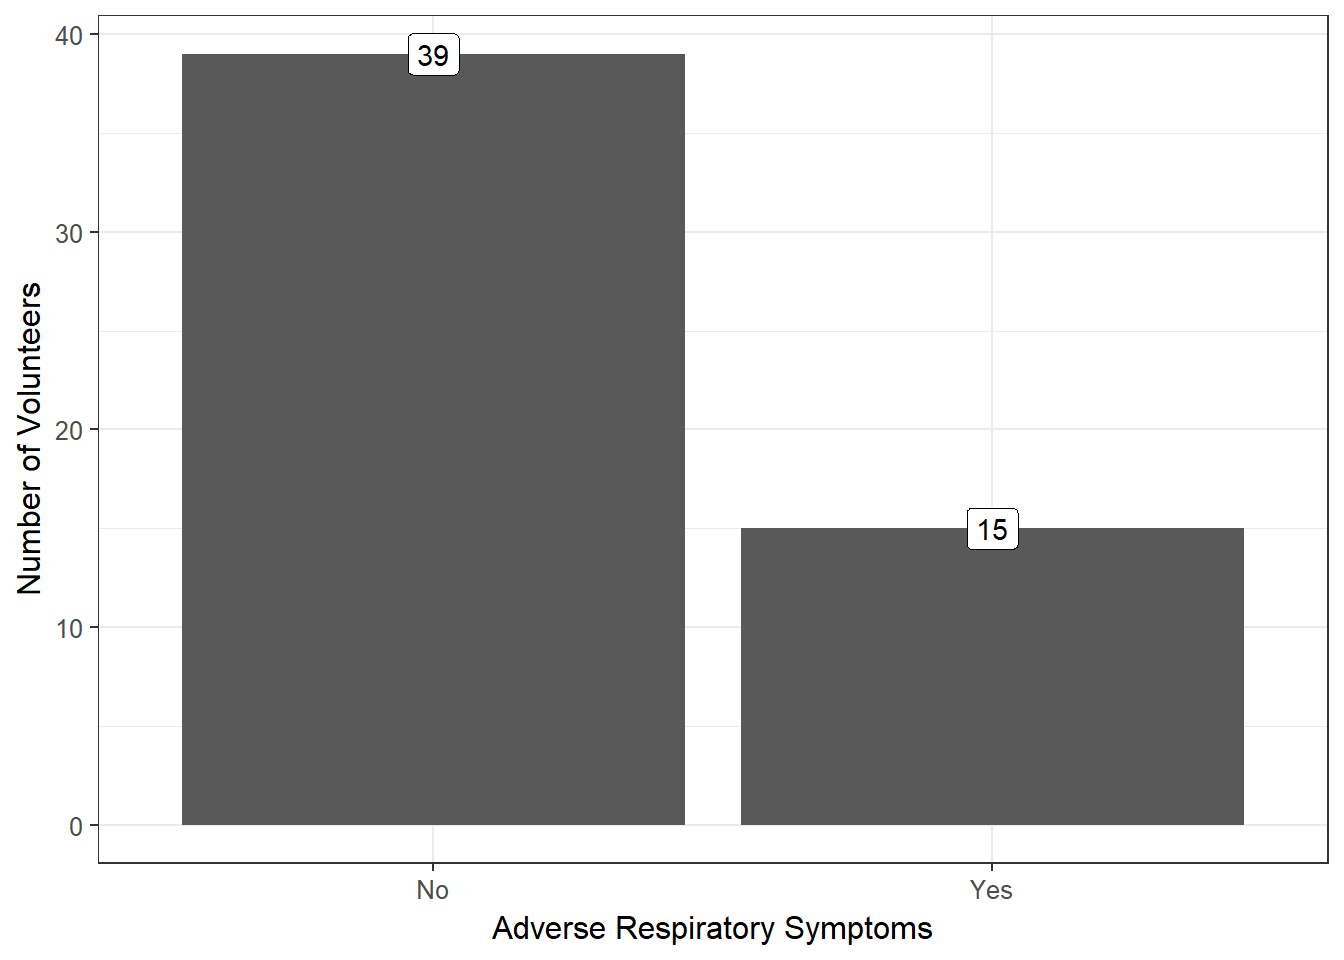
\includegraphics[width=0.8\linewidth]{./Images/summaries-deepwater-barchart-1} 

}

\caption{Frequency of adverse respiratory symptoms for volunteers cleaning wildlife following the Deepwater Horizon oil spill.}\label{fig:summaries-deepwater-barchart}
\end{figure}

In general, it does not matter whether the frequency or the relative
frequencies are reported; however, if the relative frequencies are
plotted, some indication of the sample size should be provided with the
figure either as an annotation or within the caption. Statisticians tend
to agree that bar charts are preferable to pie charts (see
\href{https://www.google.com/url?sa=t\&rct=j\&q=\&esrc=s\&source=web\&cd=32\&cad=rja\&uact=8\&ved=0ahUKEwjk6Lf42sfVAhVl64MKHaTdAFY4HhAWCC4wAQ\&url=https\%3A\%2F\%2Fwww.perceptualedge.com\%2Farticles\%2Fvisual_business_intelligence\%2Fsave_the_pies_for_dessert.pdf\&usg=AFQjCNFkS-sogmLsZIOheWAPBZSNcqjzkg}{this
whitepaper} and
\href{http://www.storytellingwithdata.com/blog/2014/06/alternatives-to-pies}{this
blog} for further explanation). More importantly, we all agree that the
graphic should help address the question. From the above graphic, we see
that nearly 28\% of volunteers assigned to wildlife experienced adverse
respiratory symptoms.

Summarizing the distribution of a numeric variable requires a bit more
thought. Consider the following example.

\BeginKnitrBlock{example}[Paper Strength]
\protect\hypertarget{exm:summaries-paper}{}{\label{exm:summaries-paper}
\iffalse (Paper Strength) \fi{} }While electronic records have become
the predominant means of storing information, we do not live in a
paperless society. Paper products are still used in a variety of
applications ranging from printing reports and photography to packaging
and bathroom tissue. In manufacturing paper for a particular
application, the strength of the resulting paper product is a key
characteristic.

There are several metrics for the strength of paper. A conventional
metric for assessing the inherent (not dependent upon the physical
characteristics, such as the weight of the paper, which might have an
effect) strength of paper is the \emph{breaking length}. This is the
length of a paper strip, if suspended vertically from one end, that
would break under its own weight. Typically reported in kilometers, the
breaking length is computed from other common measurements. For more
information on paper strength measurements and standards, see the
following website: \url{http://www.paperonweb.com}

A study was conducted at the University of Toronto to investigate the
relationship between pulp fiber properties and the resulting paper
properties (Lee \protect\hyperlink{ref-Lee1992}{1992}). The breaking
length was obtained for each of the 62 paper specimens, the first 5
measurements of which are shown in Table
\ref{tab:summaries-paper-table}. The complete data is available online
at the following website:
\url{https://vincentarelbundock.github.io/Rdatasets/doc/robustbase/pulpfiber.html}

While there are several questions one might ask with the available data,
here we are primarily interested in characterizing the breaking length
of these paper specimens.
\EndKnitrBlock{example}

\begin{table}

\caption{\label{tab:summaries-paper-table}Breaking length (km) for first 5 specimens in the Paper Strength study.}
\centering
\begin{tabular}[t]{r|r}
\hline
Specimen & Breaking Length\\
\hline
1 & 21.312\\
\hline
2 & 21.206\\
\hline
3 & 20.709\\
\hline
4 & 19.542\\
\hline
5 & 20.449\\
\hline
\end{tabular}
\end{table}

Figure \ref{fig:summaries-paper-dotplot} presents the breaking length
for all 62 paper specimens in the sample through a \emph{dot plot}.

\begin{figure}

{\centering 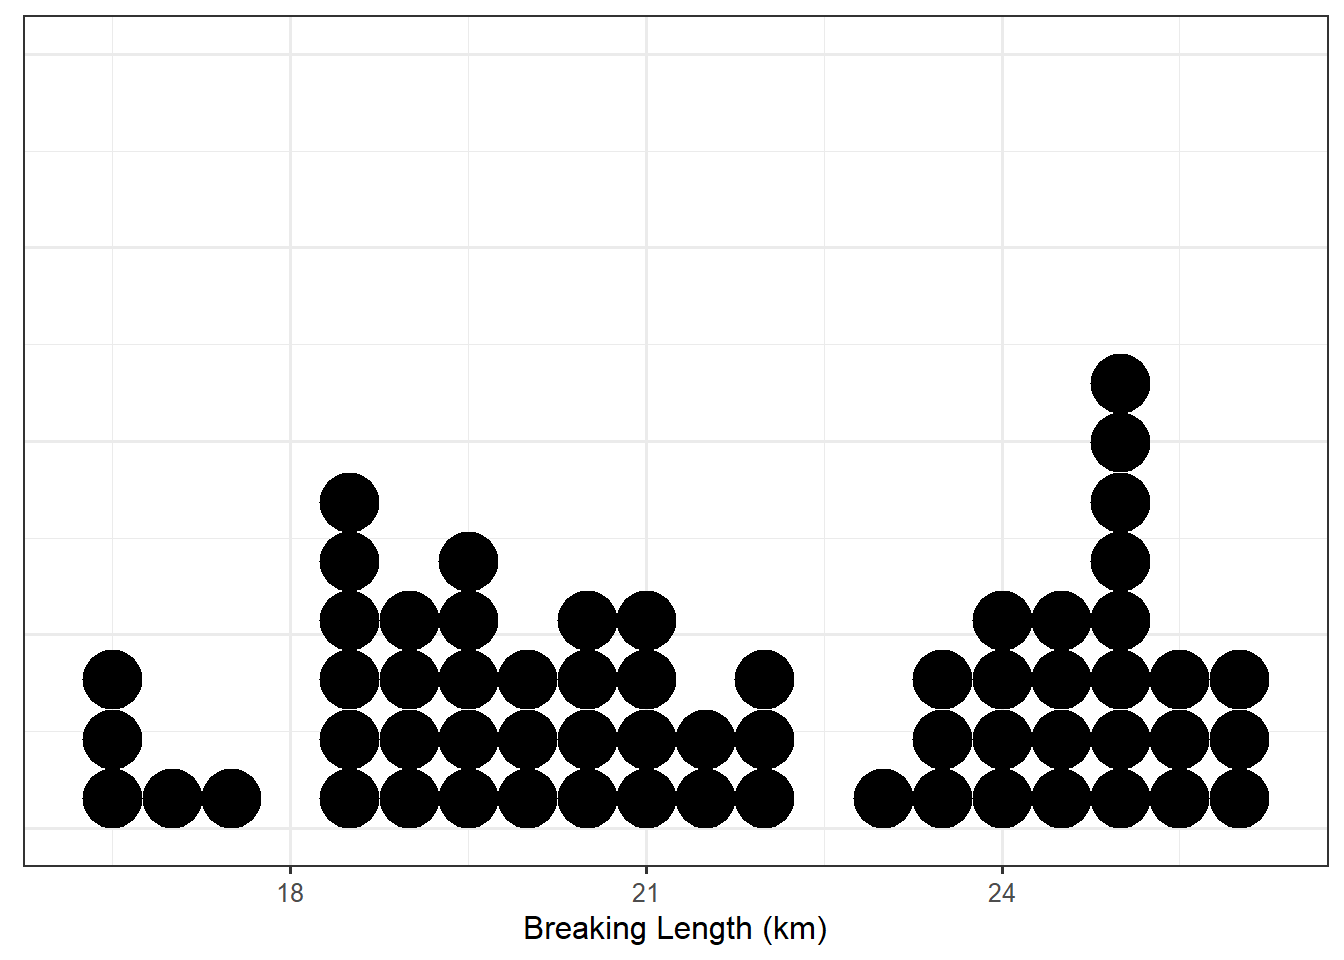
\includegraphics[width=0.8\linewidth]{./Images/summaries-paper-dotplot-1} 

}

\caption{Breaking Length (km) for 62 paper specimens.}\label{fig:summaries-paper-dotplot}
\end{figure}

With any graphic, we tend to be drawn to three components:

\begin{itemize}
\tightlist
\item
  \emph{where} the values tend to be,
\item
  \emph{how tightly} the values tend to be clustered there, and
\item
  \emph{the way} the values tend to cluster.
\end{itemize}

Notice that about half of the paper specimens in the sample had a
breaking length longer than 21.26 km. Only about 25\% of paper specimens
had a breaking length less than 19.33 km. These are measures of
\emph{location}. In particular, these are known as \textbf{percentiles},
of which the \textbf{median}, \textbf{first quartile} and \textbf{third
quartile} are commonly used examples.

\BeginKnitrBlock{definition}[Percentile]
\protect\hypertarget{def:defn-percentile}{}{\label{def:defn-percentile}
\iffalse (Percentile) \fi{} }The value \(q\) such that \(k\)\% of the
values in the distribution are less than or equal to \(q\). For example,

\begin{itemize}
\tightlist
\item
  25\% of values in a distribution are less than or equal to the 25-th
  percentile (known as the first quartile).
\item
  50\% of values in a distribution are less than or equal to the 50-th
  percentile (known as the median).
\item
  75\% of values in a distribution are less than or equal to the 75-th
  percentile (known as the third quartile).
\end{itemize}
\EndKnitrBlock{definition}

The \textbf{average} is also a common measure of location. The breaking
length of a paper specimen is 21.72 km, on average. In this case, the
average breaking length and median breaking length are very close; this
need not be the case. The average is not describing the ``center'' of
the data in the same way as the median; they capture different
properties.

\BeginKnitrBlock{definition}[Average]
\protect\hypertarget{def:defn-average}{}{\label{def:defn-average}
\iffalse (Average) \fi{} }Also known as the ``mean,'' this measure of
location represents the balance point for the distribution. It is
denoted by \(\bar{x}\).

For a sample of size \(n\), it is computed by
\[\bar{x} = \frac{1}{n}\sum_{i=1}^{n} x_i\]

where \(x_i\) rerpesents the \(i\)-th value in the sample.

When referencing the average for a population, it can also be called the
``Expected Value,'' and is often denoted by \(\mu\).
\EndKnitrBlock{definition}

Clearly, the breaking length is not equivalent for all paper specimens;
that is, there is variability in the measurements. Measures of
\emph{spread} quantify the variability of values within a distribution.
Common examples include the \textbf{standard deviation} (related to
\textbf{variance}) and \textbf{interquartile range}. For the Paper
Strength example, the breaking length varies with a standard deviation
of 2.88 km; the interquartile range for the breaking length was 5.2 km.
Neither of these values has a natural interpretation; instead, larger
values of these measures simply indicate a higher degree of variability
in the data. The standard deviation is often reported more often than
the variance since it is on the same scale as the original data;
however, as we will see later, the variance is useful from a
mathematical perspective for derivations.

\BeginKnitrBlock{definition}[Variance]
\protect\hypertarget{def:defn-variance}{}{\label{def:defn-variance}
\iffalse (Variance) \fi{} }A measure of spread, this roughly captures
the average distance values in the distribution are from the mean.

For a sample of size \(n\), it is computed by
\[s^2 = \frac{1}{n-1}\sum_{i=1}^{n} \left(x_i - \bar{x}\right)^2\]

where \(\bar{x}\) is the sample mean and \(x_i\) is the \(i\)-th value
in the sample. The division by \(n-1\) instead of \(n\) reduces the bias
in the statistic.
\EndKnitrBlock{definition}

\BeginKnitrBlock{definition}[Standard Deviation]
\protect\hypertarget{def:defn-standard-deviation}{}{\label{def:defn-standard-deviation}
\iffalse (Standard Deviation) \fi{} }A measure of spread, this is the
square root of the variance.
\EndKnitrBlock{definition}

\BeginKnitrBlock{definition}[Interquartile Range]
\protect\hypertarget{def:defn-interquartile-range}{}{\label{def:defn-interquartile-range}
\iffalse (Interquartile Range) \fi{} }The distance between the first and
third quartiles. This measure of spread indicates the range over which
the middle 50\% of the data is spread.
\EndKnitrBlock{definition}

The measures we have discussed so far are illustrated in Figure
\ref{fig:summaries-summaries}. While some authors suggest that which
values are reported depend on the shape of the distribution, we argue
that it is best to report the values that align with the question of
interest. It is the question that should be shaped by the beliefs about
the underlying distribution.

\begin{figure}

{\centering 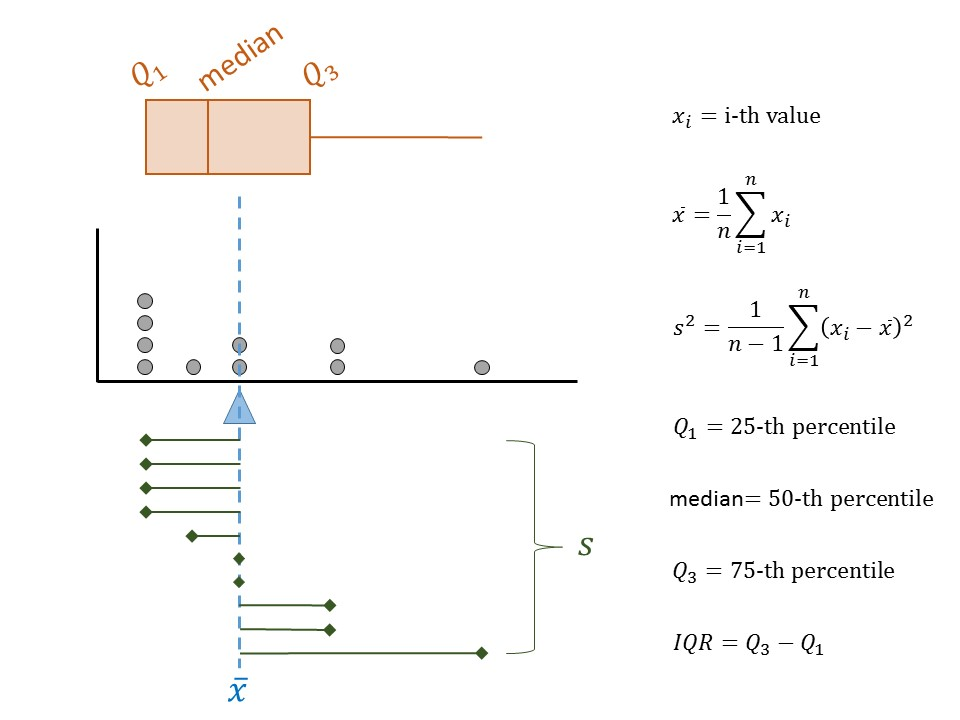
\includegraphics[width=0.8\linewidth]{./images/Summaries-Summaries} 

}

\caption{Illustration of measures of location and spread for a distribution of values.}\label{fig:summaries-summaries}
\end{figure}

Finally, consider the \emph{shape} of the distribution of breaking
length we have observed. The breaking length tends to be clustered in
two locations; we call this \emph{bimodal} (each mode is a ``hump'' in
the distribution). Other terms used to describe the shape of a
distribution are \emph{symmetric} and \emph{skewed}. Symmetry refers to
cutting a distribution in half (at the median) and the lower half being
a mirror image of the upper half; skewed distributions are those which
are not symmetric.

Observe then that the dot plot above gives us some idea of the location,
spread, and shape of the distribution, in a way that the table of values
could not. This makes it a useful graphic as it is characterizing the
\textbf{distribution of the sample} we have observed. This is one of the
distributions in what we call the \emph{Distributional Quartet}.

\BeginKnitrBlock{definition}[Distribution of the Sample]
\protect\hypertarget{def:defn-distribution-sample}{}{\label{def:defn-distribution-sample}
\iffalse (Distribution of the Sample) \fi{} }The pattern of variability
in the observed values of a variable.
\EndKnitrBlock{definition}

When the sample is not large, a dot plot is reasonable. Other common
visualizations for a single variable include a \emph{jitter plot},
\emph{box plot}, \emph{histogram}, or \emph{density plot} (smoothed
histogram). To illustrate, the breaking length for the Paper Strength
example is summarized using various methods in Figure
\ref{fig:summaries-univariate}. The latter three visualizations are more
helpful when the dataset is very large and plotting the raw values
actually hides the distribution. There is no right or wrong graphic; it
is about choosing the graphic which addresses the question and
adequately portrays the distribution.

\begin{figure}

{\centering 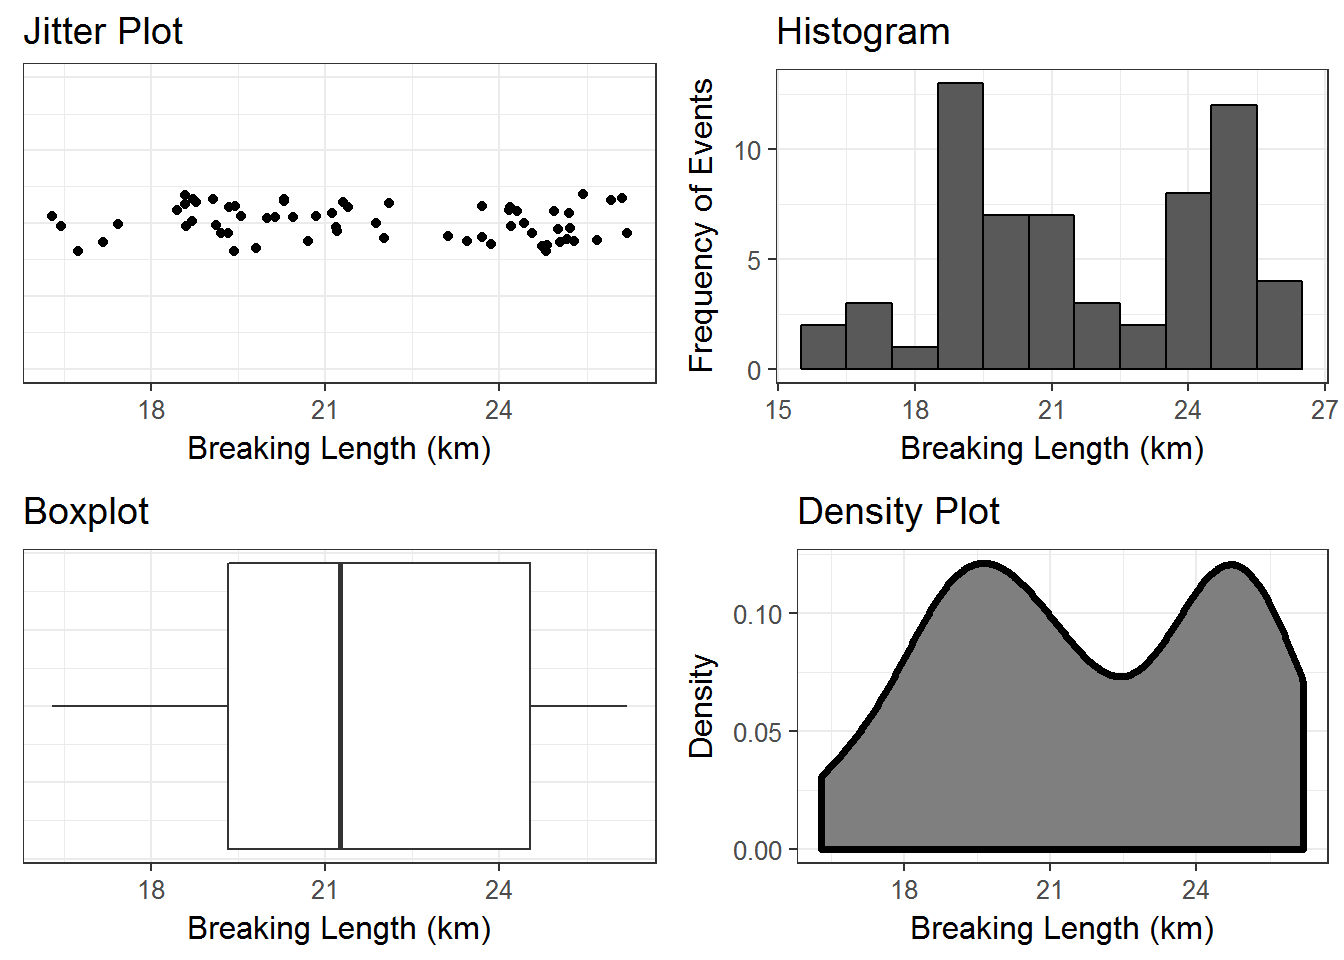
\includegraphics[width=0.8\linewidth]{./Images/summaries-univariate-1} 

}

\caption{Four graphical summaries of the breaking length for the Paper Strength example.}\label{fig:summaries-univariate}
\end{figure}

The numeric summaries of a distribution are known as
\textbf{statistics}. While parameters characterize a variable at the
population level, statistics characterize a variable at the sample
level.

\BeginKnitrBlock{definition}[Statistic]
\protect\hypertarget{def:defn-statistic}{}{\label{def:defn-statistic}
\iffalse (Statistic) \fi{} }Numeric quantity which summarizes the
distribution of a variable within a \emph{sample}.
\EndKnitrBlock{definition}

Why would we compute numerical summaries in the sample if we are
interested in the population? Remember the goal of this discipline is to
use the sample to say something about the underlying population. As long
as the sample is representative, the distribution of the sample should
reflect the \textbf{distribution of the population}; therefore,
summaries of the sample should roughly equate to the analogous summaries
of the population. Now we see the real importance of having a
representative sample; it allows us to say that what we observe in the
sample is a good proxy for what is happening in the population.

\BeginKnitrBlock{definition}[Distribution of the Population]
\protect\hypertarget{def:defn-distribution-population}{}{\label{def:defn-distribution-population}
\iffalse (Distribution of the Population) \fi{} }The pattern of
variability in values of a variable at the population level. Generally,
this is impossible to know, but we might model it.
\EndKnitrBlock{definition}

That is, the mean in the sample should approximate (estimate) the mean
in the population; the standard deviation of the sample should estimate
the standard deviation in the population; and, the shape of the sample
should approximate the shape of the population, etc. The sample is
acting as a representation in all possible ways of the population.

\BeginKnitrBlock{rmdkeyidea}
A representative sample reflects the population; therefore, we can use
statistics as estimates of the population parameters.
\EndKnitrBlock{rmdkeyidea}

\section{Summarizing Relationships}\label{summarizing-relationships}

The summaries discussed above are nice for examining a single variable.
In general, research questions of interest typically involve the
relationship between two or more variables. Most graphics are
two-dimensional (though 3-dimensional graphics and even virtual reality
are being utilized now); therefore, summarizing a rich set of
relationships may require the use of both axes, color, shape, size, and
even multiple plots in order to tell the right story. We will explore
these various features in upcoming units of the text. Here, we focus on
the need to tell a story that answers the question of interest instead
of getting lost in making a graphic. Consider the following question
from the \protect\hyperlink{CaseDeepwater}{Deepwater Horizon Case
Study}:

\begin{quote}
What is the increased risk of developing adverse respiratory symptoms
for volunteers cleaning wildlife compared to those volunteers who do not
have direct exposure to oil?
\end{quote}

Consider the graphic in Figure \ref{fig:summaries-bad-barchart}; this is
\emph{not} a useful graphic. While it compares the number of volunteers
with symptoms in each group, we cannot adequatly address the question
because the research question involves comparing the rates for the two
groups.

\begin{figure}

{\centering 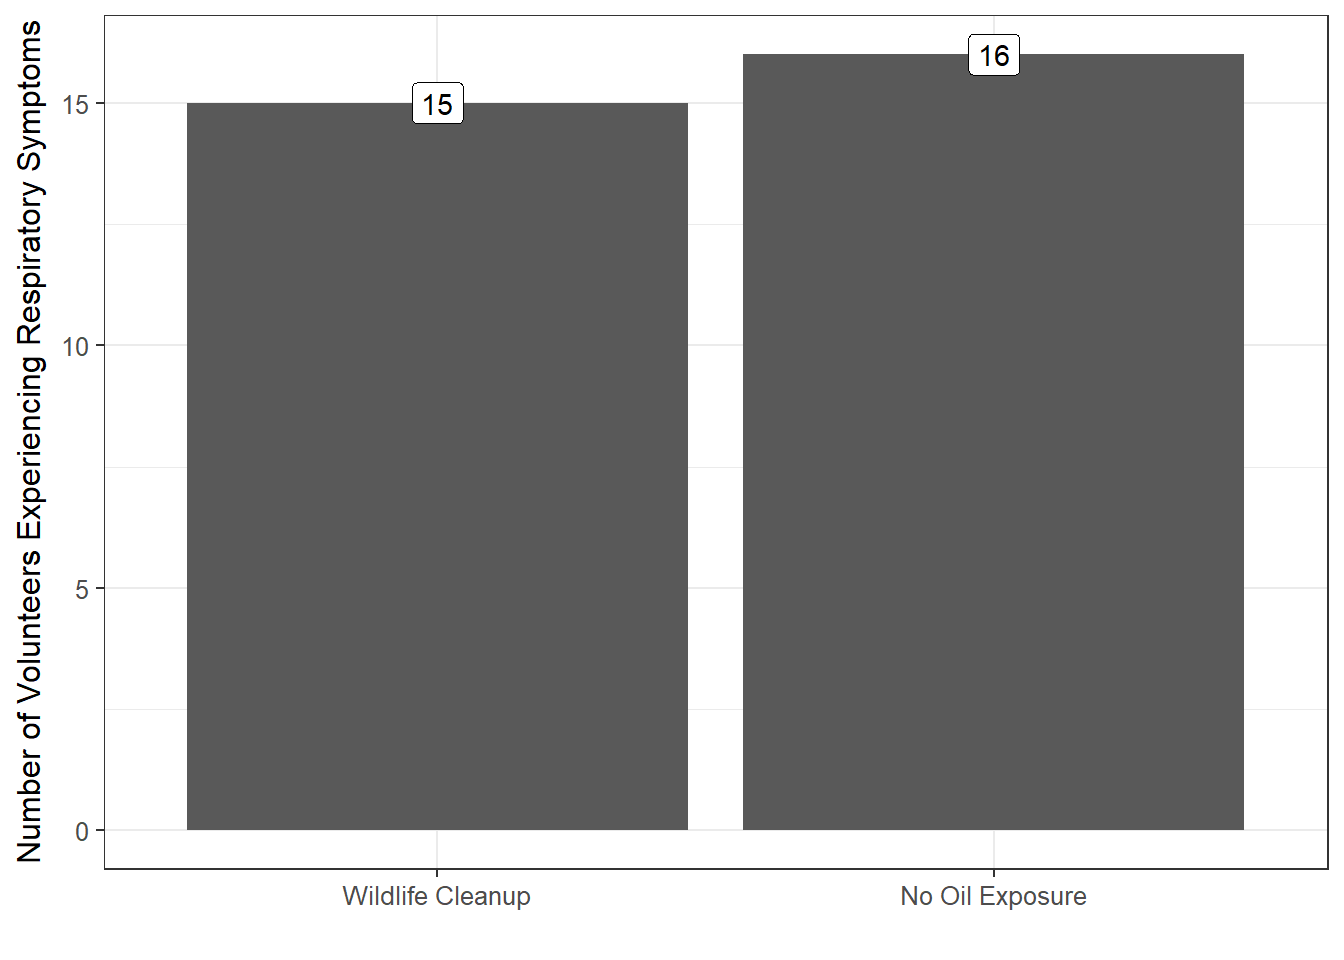
\includegraphics[width=0.8\linewidth]{./Images/summaries-bad-barchart-1} 

}

\caption{Illustration of a poor graphic; the graphic does not give us a sense of the rate within each group in order to make a comparison.}\label{fig:summaries-bad-barchart}
\end{figure}

Instead, Figure \ref{fig:summaries-good-barchart} compares the rates
within each group. Notice that since we are reporting relative
frequencies for comparison, we report the sample size for each group.

\begin{figure}

{\centering 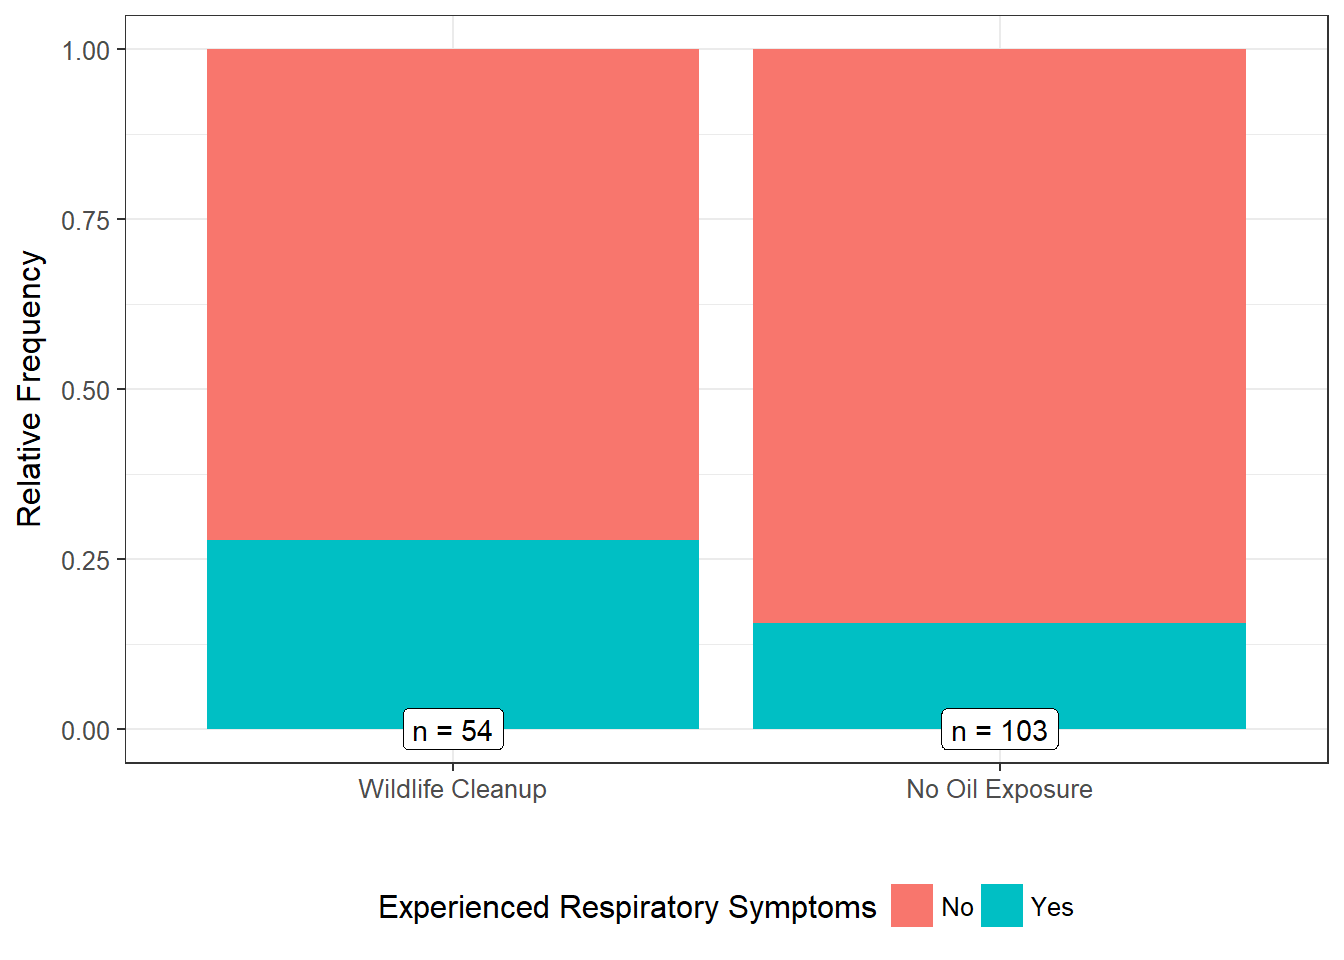
\includegraphics[width=0.8\linewidth]{./Images/summaries-good-barchart-1} 

}

\caption{Comparison of the rate of adverse respiratory symptoms among volunteers assigned to different tasks.}\label{fig:summaries-good-barchart}
\end{figure}

From the graphic, it becomes clear that a higher fraction of volunteers
cleaning wildlife experienced adverse symptoms compared with those
without oil exposure. In fact, volunteers cleaning wildlife were 1.79
times more likely to experience adverse respiratory symptoms.

The key to a good summary is understanding the question of interest and
addressing this question through a useful characterization of the
variability.

\chapter{Assessing the Evidence (Quantifying the Variability in
Estimates)}\label{SamplingDistns}

Again, the goal of statistical inference is to use the sample as a
snapshot of the underlying population (Figure
\ref{fig:samplingdistns-statistical-process}). There are generally three
reasons people distrust this process:

\begin{enumerate}
\def\labelenumi{\arabic{enumi}.}
\tightlist
\item
  Fear that the sample does not represent what is going on in the
  population.
\item
  Fear that we cannot make a conclusion with a sample of size \(n\)
  (wanting more data).
\item
  Fear that one study is not enough to make a conclusion.
\end{enumerate}

\begin{figure}

{\centering 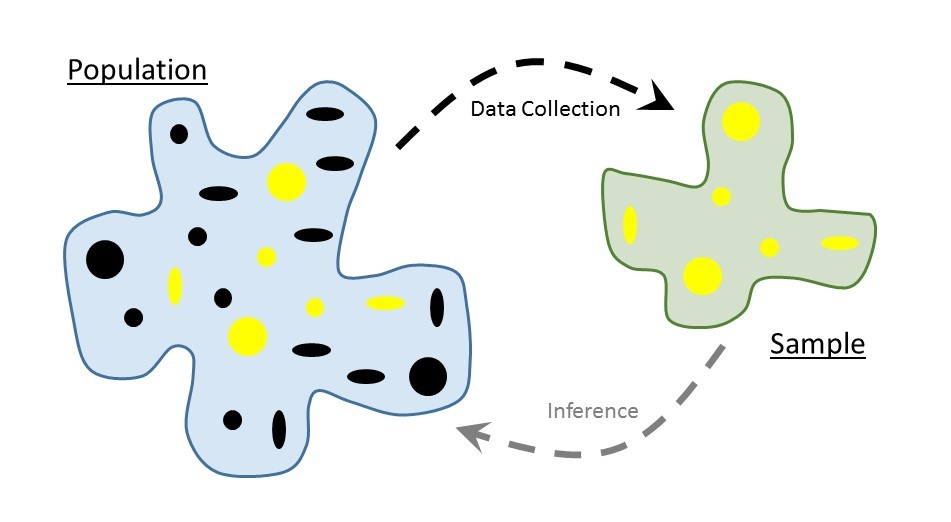
\includegraphics[width=0.8\linewidth]{images/Basics-Stat-Process} 

}

\caption{Illustration of the statistical process (reprinted from Chapter 1).}\label{fig:samplingdistns-statistical-process}
\end{figure}

We have already tackled the first reason in Chapter @ref(\#Data); if we
are to trust statistical results, we must collect data that is
representative of the underlying population. The second and third fears
above are tied together, though maybe not obviously. Before launching
into a slightly more formal discussion, consider the following thought
experiment.

\BeginKnitrBlock{example}[Free Throws]
\protect\hypertarget{exm:samplingdistns-free-throws}{}{\label{exm:samplingdistns-free-throws}
\iffalse (Free Throws) \fi{} }Your friends Dave lives for his Wednesday
``pick-up'' basketball games at the gym. One afternoon, while waiting
for a few more players to arrive Dave shoots 10 free throws, of which he
makes 3.
\EndKnitrBlock{example}

I imagine no one is ready to claim \emph{definitively} that Dave has a
30\% success rate from the free throw line. So, what can we say? Well,
if this set of 10 free throws is representative of Dave's free throw
performance, then we would say that 30\% is an estimate for his success
rate; that is, the statistic 30\% is a good guess at the unknown
parameter (overall success rate). There are two ways we might impove our
confidence in this estimate. First, we might consider a larger sample
size (make Dave shoot more free throws).

\BeginKnitrBlock{example}[Free Throws (cont.)]
\protect\hypertarget{exm:samplingdistns-free-throws2}{}{\label{exm:samplingdistns-free-throws2}
\iffalse (Free Throws (cont.)) \fi{} }Joe has also been waiting for a
few more players to arrive; however, Joe shoots 100 free throws (clearly
he has more time on his hands) of which he makes 30.
\EndKnitrBlock{example}

Again, we probably wouldn't claim \emph{definitively} that Joe has a
30\% success rate from the free throw line. But, assuming this set of
100 free throws is representative of his overall performance, then we
would be more confident in our guess for Joe's overall performance
compared with our guess for Dave's. The more shots we observe, the more
confidence we have in our estimate. This idea is known as the
\textbf{Law of Large Numbers}.

\BeginKnitrBlock{definition}[Law of Large Numbers]
\protect\hypertarget{def:defn-lln}{}{\label{def:defn-lln} \iffalse (Law of
Large Numbers) \fi{} }For our purposes, this essentially says that as a
sample size gets really large, a statistic will become arbitrarily close
(extremely good guess) of the parameter it estimates.
\EndKnitrBlock{definition}

Unfortunately, we may not be able to take a really large sample. It is
probably not feasible to have Dave or Joe shoot thousands of free
throws, for example. Our goal then becomes to somehow quantify the
confidence we have in our estimates \emph{given the sample size we have
available}. That is, given that we only saw Dave shoot 10 free throws,
can we quantify our confidence in that 30\% estimate of his free throw
success? Our ``confidence'' in an estimate is tied to the estimate's
repeatability --- ``if we were to repeat the study, how much would we
expect our estimate to change?'' This gets at the last fear; we know
that if we repeat a study, the results will change. Our job is to
quantify (keeping the sample size in mind) the degree to which the
results will change. That is, we need to quantify the \emph{variability}
in the estimate across repeated studies (known as sampling variability;
we told you statistics was all about variability). This is known as a
\textbf{sampling distribution}.

\BeginKnitrBlock{definition}[Sampling Distribution]
\protect\hypertarget{def:defn-sampling-distribution}{}{\label{def:defn-sampling-distribution}
\iffalse (Sampling Distribution) \fi{} }The distribution of a
\emph{statistic} across repeated samples.
\EndKnitrBlock{definition}

This is perhaps the most important of the \emph{Distributional Quartet};
it is the holy grail of statistical inference. Once we have the sampling
distribution, inference is straight-forward.

\BeginKnitrBlock{rmdfivefund}
\textbf{Fundamental Idea IV}: Variability is inherent in any process,
and as a result, our estimates are subject to sampling variability.
However, these estimates often vary across samples in a predictable way;
that is, they have a distribution that can be modeled.
\EndKnitrBlock{rmdfivefund}

\section{Conceptualizing the Sampling
Distribution}\label{conceptualizing-the-sampling-distribution}

The sampling distribution of a statistic is one of the most fundamental,
and yet one of the most abstract, concepts in statistics. It's name is
even confusing; the ``distribution of the sample'' (Definition
\ref{def:defn-distribution-sample}) and the ``sampling distribution''
(Definition \ref{def:defn-sampling-distribution}) are two different
things. In this section, we develop the idea of a sampling distribution;
then, we turn toward actually constructing it.

For the \protect\hyperlink{DeepwaterCase}{Deepwater Horizon Case Study},
consider the following question:

\begin{quote}
What proportion of volunteers assigned to clean wildlife will develop
adverse respiratory symptoms?
\end{quote}

In the sample, we observed 15 out of 54 such volunteers (27.8\% or a
proportion of 0.278). This proportion is a good estimate of the rate of
adverse symptoms in the population (assuming the sample is
representative, of course). Now, imagine randomly selecting 54 new
volunteers from the population (repeating the study). We could determine
what fraction of volunteers in this new sample experienced adverse
symptoms, expecting this value to be a bit different than what we
obtained in the first sample. Since this second sample is also
representative, it provides a good estimate of the parameter. Now, we
could take a third random sample of 54 volunteers and compute the
fraction in this third sample which experienced adverse symptoms. This
third sample also provides a good (and potentially unique) estimate of
the parameter. We could continue this process \(m\) times, for some
large number \(m\). This process is illustrated in Figure
\ref{fig:samplingdistns-sampling-distribution}.

\begin{figure}

{\centering 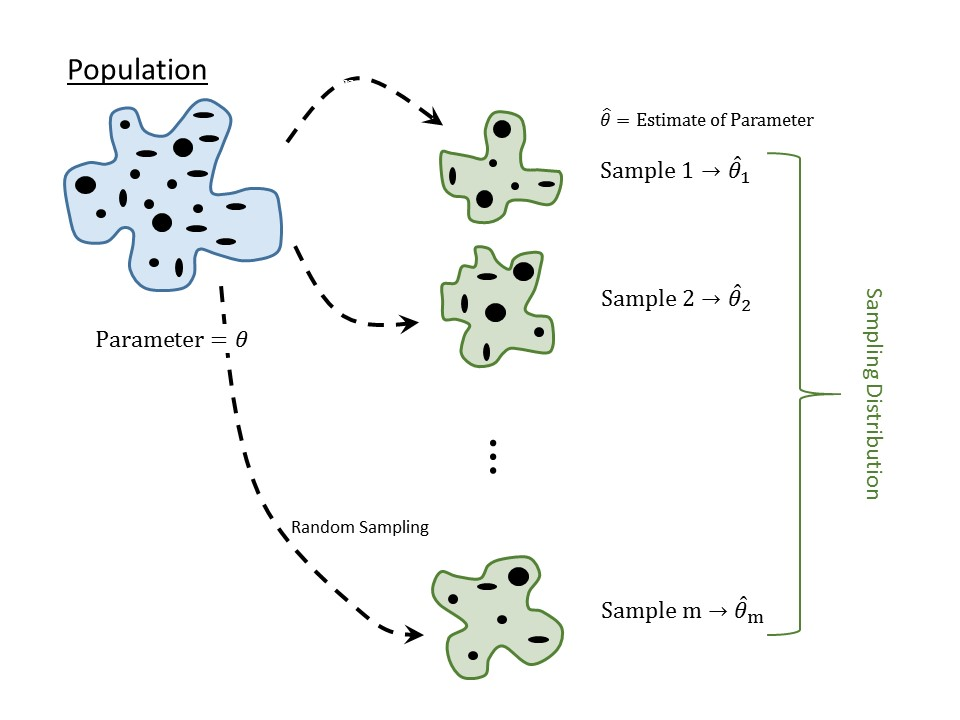
\includegraphics[width=0.8\linewidth]{./images/SamplingDistns-Sampling-Distribution} 

}

\caption{Illustration of repeatedly sampling from a population.}\label{fig:samplingdistns-sampling-distribution}
\end{figure}

Consider what we are describing. With each representative sample, we
have constructed an estimate of the parameter. What we have kept from
each repetion is \emph{not} the values of the variables themselves
(whether the volunteers experienced adverse respiratory symptoms) but
rather we have retained the \emph{statistic} from each of \(m\) whole
new studies. So, which of these \(m\) estimates do we trust? All of
them. Since each sample is representative of the population, each
estimate is a good (not perfect) estimate of the parameter. Since we
have all these estimates, we could think about pooling the information
from all of them; describing the way in which they change from one
sample to another is the sampling distribution.

Notice that the sampling distribution is not describing a variable, it
is describing a \emph{statistic}. In order to construct a sampling
distribution, we would go through the following steps:

\begin{enumerate}
\def\labelenumi{\arabic{enumi}.}
\tightlist
\item
  Take a sample; record variables of interest.
\item
  Compute the statistic which estimates the parameter.
\item
  Repeat steps 1 and 2 a large number of times.
\item
  Examine the statistics collected.
\end{enumerate}

So, the sampling distribution is not a plot of the raw values of a
variable on individual subjects but a plot of statistics which summarize
entire samples. That is, the unit of observation has changed. While a
sample consists of individual subjects from the population, the sampling
distribution consists of individual samples from the population.

\BeginKnitrBlock{rmdtip}
Re-read the description of a sampling distribution several times, and
return to it often as you read through the text. It takes a while for
this to sink in, but if you truly grasp this one concept, the remainder
of statistical inference becomes much more accessible.
\EndKnitrBlock{rmdtip}

\section{Example of a Sampling
Distribution}\label{example-of-a-sampling-distribution}

Since this idea is so critical to grasping statistical inference, we are
going to walk through the process of generating a sampling distribution
for a known data generating process.

\BeginKnitrBlock{example}[Dice Experiment]
\protect\hypertarget{exm:samplingdistns-dice}{}{\label{exm:samplingdistns-dice}
\iffalse (Dice Experiment) \fi{} }Consider an ordinary six-sided die; we
are interested in the proportion of times that rolling the die will
result in a 1. Putting this in the language of the statistics, we have
the following:

\begin{itemize}
\tightlist
\item
  The \emph{population} of interest is all rolls of the die. Notice that
  this population is infinitely large as we could roll the die forever.
\item
  The \emph{variable} is the resulting value from the roll. Since this
  can take on only one of six values, this is a categorical variable.
\item
  The \emph{parameter} of interest is the proportion of rolls that
  result in a 1.
\end{itemize}

Our goal is to construct the sampling distribution of the proportion of
rolls that result in a 1 when the die is rolled 20 times.
\EndKnitrBlock{example}

What makes this example unique is that we know the value of the
parameter. Because of the physical properties of a die, we know that the
probability a roll results in a 1 is \(\theta = 1/6\). So, statistical
inference is not needed here. This example simply provides a simple
vehicle for studying sampling distributions. Going back to the steps for
creating a sampling distribution described in the previous section, we
have the following steps:

\begin{enumerate}
\def\labelenumi{\arabic{enumi}.}
\tightlist
\item
  Roll a die 20 times, each time recording the resulting value.
\item
  Compute the proportion of times (out of the 20) the resulting value
  was a 1.
\item
  Repeat steps 1 and 2 a large number of times (let's say 500).
\item
  Plot the resulting values; there should be 500 proportions that we are
  keeping.
\end{enumerate}

Notice that we are actually rolling a die 10000 times (20 rolls repeated
500 times); we only keep 500 values (one proportion for each set of 20
rolls). This is something you could physically do at home. For example,
the first sample might look like that in Figure
\ref{fig:samplingdistns-dice-example}.

\begin{figure}

{\centering 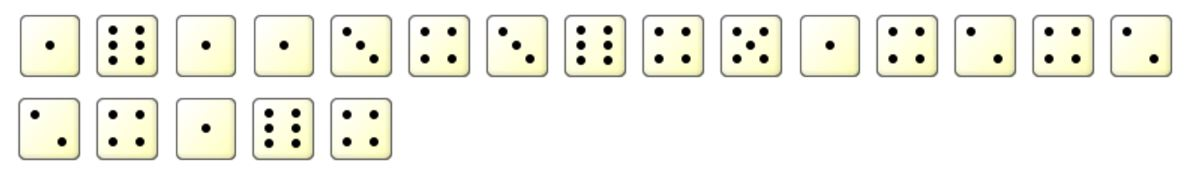
\includegraphics[width=0.8\linewidth]{./images/SamplingDistns-Dice-Example} 

}

\caption{Potential sample of rolling a cie 20 times.}\label{fig:samplingdistns-dice-example}
\end{figure}

For this particular sample, the proportion in the sample (our statistic
of interest) would be 0.25 (\(5/20\)). That is the value we would
record. We then repeat this 499 more times. You could try a few out
yourself using \href{https://www.random.org/dice/?num=20}{an online
simulator}. Figure \ref{fig:samplingdistns-dice-dotplot} shows the
resulting proportions for 500 samples of size 20 each.

\begin{figure}

{\centering 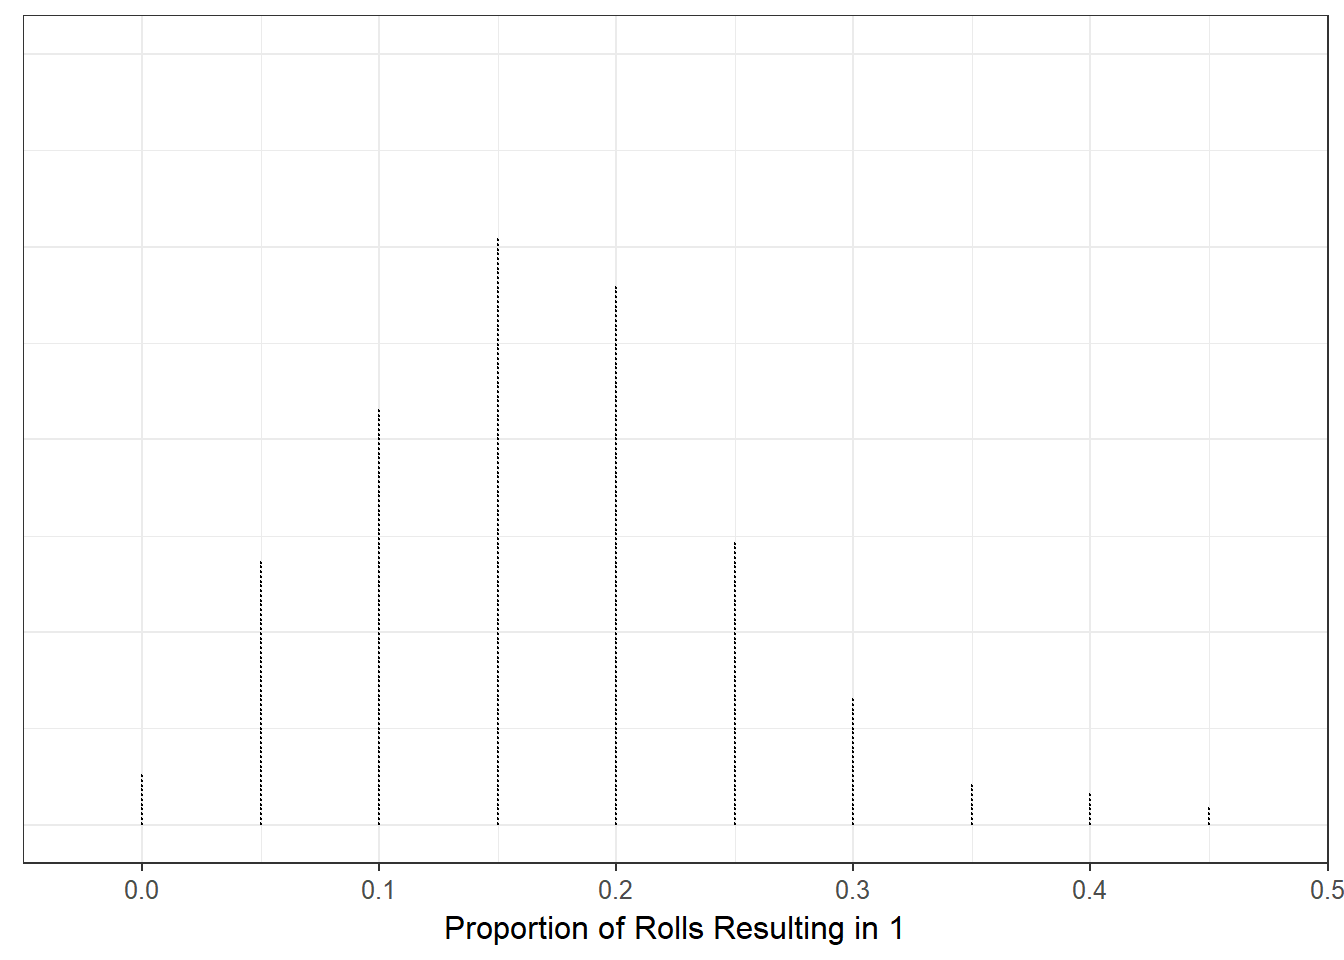
\includegraphics[width=0.8\linewidth]{./Images/samplingdistns-dice-dotplot-1} 

}

\caption{Sampling distribution for the proportion of 20 dice rolls which result in a 1.  The distribution is based on repeating the sampling process 500 times.}\label{fig:samplingdistns-dice-dotplot}
\end{figure}

With modern computing power, there is no need to restrain ourselves to
repeating the study 500 times. A simple computer program could replicate
rolling the dice thousands of times. Figure
\ref{fig:samplingdistns-dice-histogram} is the sampling distribution for
the proportion of rolls that result in a 1 based on a sample of size 20
repeating the study 50000 times.

\begin{figure}

{\centering 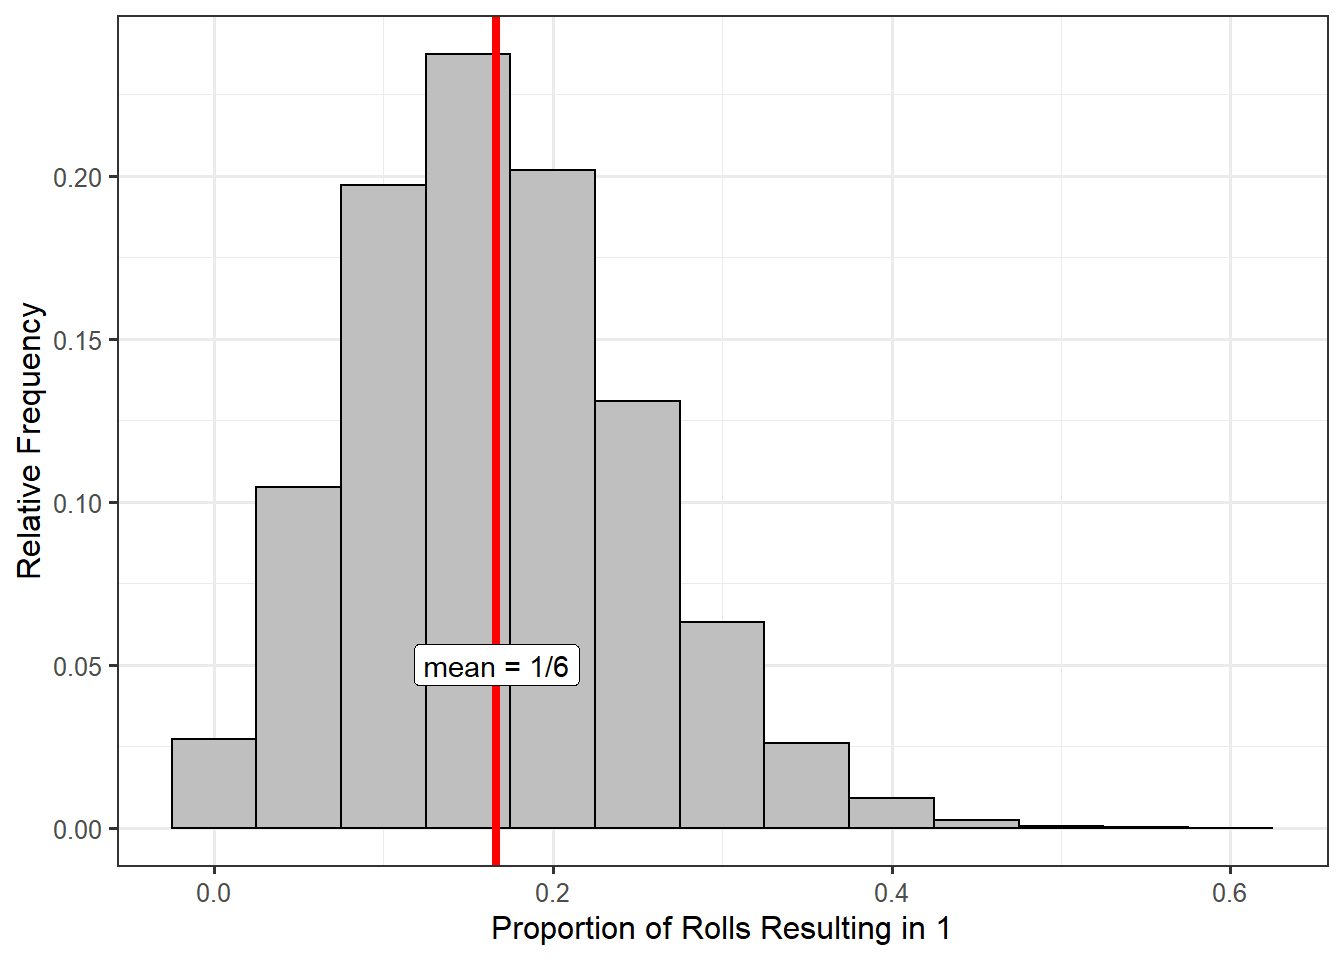
\includegraphics[width=0.8\linewidth]{./Images/samplingdistns-dice-histogram-1} 

}

\caption{Sampling distribution for the proportion of 20 dice rolls which result in a 1.  The distribution is based on repeating the sampling process 50000 times.}\label{fig:samplingdistns-dice-histogram}
\end{figure}

Notice that the sampling distribution is centered around the true value
of the parameter (\(\theta = 1/6\)). In general, the sampling
distribution of statistics, when taken from a random sample, center on
the true value of the parameter. This is the unbiased nature of the data
coming out; random samples are representative of the population.
Similarly, note that while no one sample (remember, each value in the
distribution represents a statistic from a sample of 20 values) is
perfect, no samples produce values which are far from the true
parameter. That is, a representative sample may not be perfect, but it
will give a \emph{reasonable} estimate of the parameter. Notice that
these properties hold even though we had a relatively small sample size
(\(n = 20\) coin flips).

\BeginKnitrBlock{rmdkeyidea}
The size of the sample is not as important as whether it is
representative. A small representative sample is better for making
inference than a large sample which is biased.
\EndKnitrBlock{rmdkeyidea}

One of the most useful things about the sampling distribution is that it
gives us an idea of how much we might expect our statistic to change
from one sample to another. Based on Figure
\ref{fig:samplingdistns-dice-histogram}, we could say that if we roll a
die 20 times, the proportion of rolls which result in a 1 is most likely
to be between 0.05 and 0.30 (so somewhere between 1 and 6 ones out of
the 20 rolls). It would be \emph{extremely} rare to have 12 of the 20
rolls result in a 1 (notice how small the bar is on the 0.6 proportion).
The sampling distribution is therefore giving us an idea of the
variability in our statistic.

Remember, our goal was to account for the variability in the statistic
(how much it changes from one sample to another) \emph{while accounting
for the sample size}. How is this done? When forming the sampling
distribution, we repeated the study. For each replication, we obtained a
new sample that \emph{had the same size as the original}. So, the sample
size is baked into the sampling distribution. To see the impact of
taking a larger sample, consider rolling a six-sided die 60 times
instead of 20 times. When we build the sampling distribution, each
replication will then involve repeating the process with 40 new rolls.
Figure \ref{fig:samplingdistns-dice-histogram2} shows the sampling
distribution of the proportion of 60 rolls which result in a 1 using
50000 replications. Notice that the distribution is still centered on
the true parameter \(\theta = 1/6\). The primary difference between this
figure and the last is that when we increased the sample size, the
sampling distribution narrowed.

\begin{figure}

{\centering 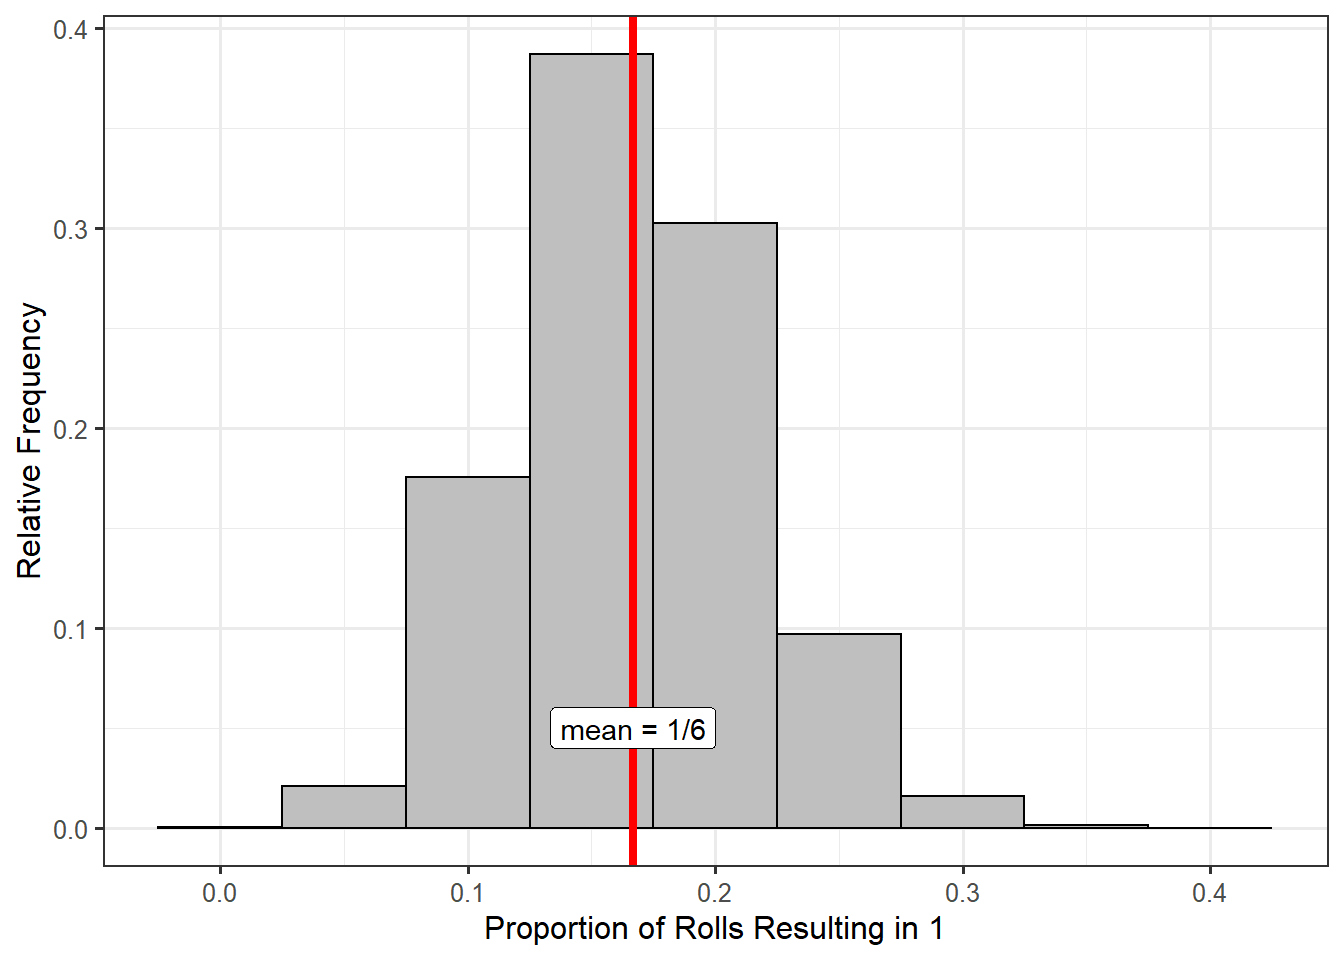
\includegraphics[width=0.8\linewidth]{./Images/samplingdistns-dice-histogram2-1} 

}

\caption{Sampling distribution for the proportion of 60 dice rolls which result in a 1.  The distribution is based on repeating the sampling process 50000 times.}\label{fig:samplingdistns-dice-histogram2}
\end{figure}

We all have this intuition that ``more data is better.'' In truth, we
should say ``more \emph{good} data is better.'' By ``better,'' we mean
that the statistic is less variable. Notice that we have to be careful
here. We are not saying that the \emph{sample} has less variability; we
are saying the \emph{statistic} has less variability. That is, we are
more confident in our estimate because we do not expect it to change as
much from one sample to the next. From Figure
\ref{fig:samplingdistns-dice-histogram2}, we have that if we roll the
die 60 times, we expect the proportion of 1's to be somewhere between
0.1 and 0.25 (somewhere between 6 and 15 ones out of the 60 show up).
The proportion is varying much less from one sample to the next.

\BeginKnitrBlock{rmdkeyidea}
Larger samples result in \emph{statistics} which are less variable. This
shows itself in the sense that the sampling distribuiton is narrower.
\EndKnitrBlock{rmdkeyidea}

\BeginKnitrBlock{rmdtip}
Students often believe that a large sample reduces the variability in
the data. That is not true; a large sample reduces the variability in
the \emph{statistic}.
\EndKnitrBlock{rmdtip}

\section{Modeling the Sampling
Distribution}\label{modeling-the-sampling-distribution}

Let's return to the \protect\hyperlink{CaseDeepwater}{Deepwater Horizon
Case Study}. In particular, suppose we are tyring to address the
following question:

\begin{quote}
What proportion of volunteers assigned to clean wildlife will develop
adverse respiratory symptoms?
\end{quote}

We have an estimate for this proportion (\(p = 0.278\)) based on the
observed sample. Based on the discussion in the previous section, we
know the sampling distribution of this proportion can help us quantify
the variability in the estimate. Figure
\ref{fig:samplingdistns-deepwater-histogram} represents the sampling
distribution of this proportion. From the graphic, we would not expect
the proportion of volunteers who experience adverse respiratory symptoms
to move much beyond 0.15 and 0.4 if we were to repeat the study; it
would almost certainly not move beyond 0.1 and 0.5 if we were to repeat
the study.

\begin{figure}

{\centering 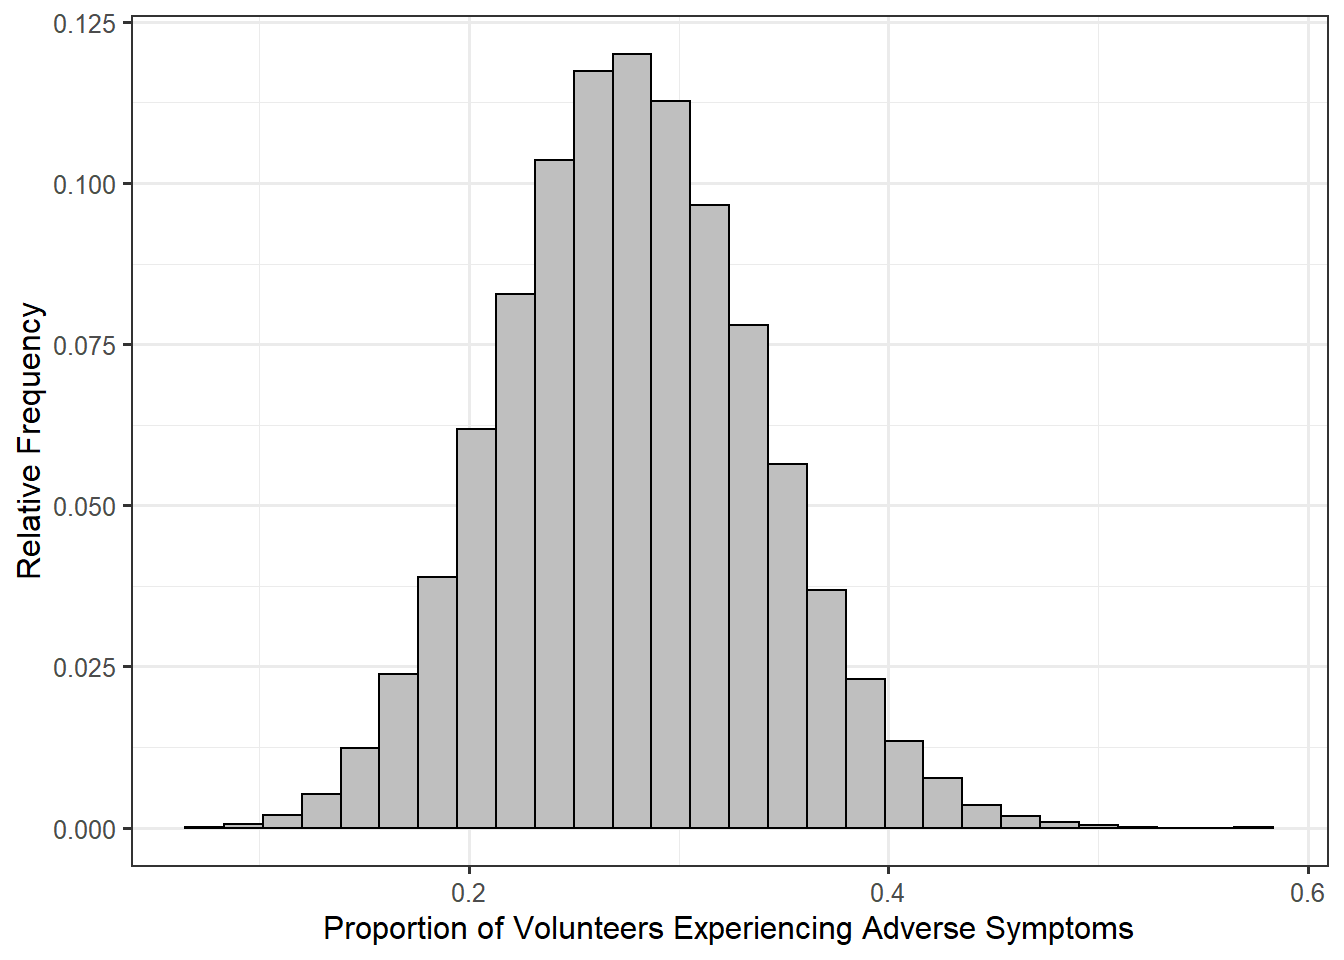
\includegraphics[width=0.8\linewidth]{./Images/samplingdistns-deepwater-histogram-1} 

}

\caption{Sampling distribution for the proportion of volunteers assigned to wildlife who will develop adverse symptoms based on a sample of 54 volunteers.}\label{fig:samplingdistns-deepwater-histogram}
\end{figure}

Now, you might ask ``wait, where did this sampling distribution come
from? There is no way you actually repeated the study 50000 times,
right?'' Right. In the previous section, we described building the
sampling distribution through repeated sampling. But, in practice, this
is never practical; if it were, we would have just conducted a bigger
sample to begin with. Generally, cost is the limiting factor in choosing
a sample size; so, we only have a limited set of data to work with. So,
the sampling distribution is critical to making inference, but we cannot
take multiple samples to make it. Where does that leave us? The
answer\ldots{}modeling. Our goal is to construct a model of the sampling
distribution that we can use to make inference.

There are three general techniques for modeling the sampling
distribution of a statistic:

\begin{enumerate}
\def\labelenumi{\arabic{enumi}.}
\tightlist
\item
  Build an empirical model.
\item
  Build an analytical model using probability theory.
\item
  Build an analytical model appealing to approximations.
\end{enumerate}

We will focus on the first approach; the latter two approaches are
discussed in the last unit of the text. The idea in constructing an
empirical model is to mimic the discussion above regarding the
construction of a sampling distribution. Our description references
Figure \ref{fig:samplingdistns-bootstrap} often. We are limited by our
resources; because of time and money constraints, we cannot resample
from the population (crossed off resamples). So, we pretend for a moment
that our original sample (colored in green in the figure) is the
population for a moment. Our idea is to randomly sample from this
original sample, creating a \emph{bootstrap resample} (colored in orange
in the figure). Forgive the non-technical terms here, but since the
orange ``blob'' is a random sample from the green ``blob,'' then it is
representative of the green blob. Therefore, if we construct an estimate
\(\widehat{\theta}^*\) from the orange blob (the star denotes a
statistic from a resample), then it should be close to the statistic
\(\widehat{\theta}\) from the green blob; but, since this green blob is
representative of the population, \(\widehat{\theta}\) should be close
to the true parameter \(\theta\). Therefore, we have that \[
\widehat{\theta}^* \approx \widehat{\theta} \approx \theta \Rightarrow \widehat{\theta}^* \approx \theta
\]

That is, the bootstrap resamples produce statistics which are good
estimates of the parameter from the underlying population. The benefit
here is that the bootstrap resamples are constructed in the computer.
And, given today's computing power, we are not limited by time or money
(10000 bootstrap resamples can often be taken in a matter of seconds).
If you want to see this process in action, we encourage you to check out
the free online app located at
\url{http://www.lock5stat.com/StatKey/bootstrap_1_cat/bootstrap_1_cat.html}.

\begin{figure}

{\centering 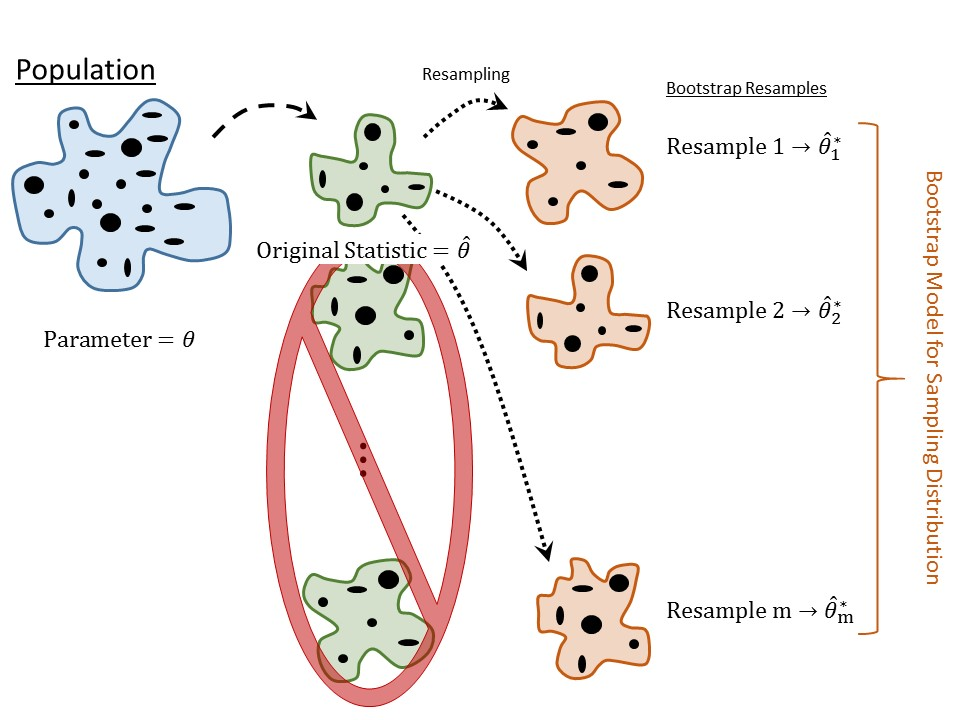
\includegraphics[width=0.8\linewidth]{./images/SamplingDistns-Bootstrap} 

}

\caption{Illustration of modeling the sampling distribution via the Bootstrap.}\label{fig:samplingdistns-bootstrap}
\end{figure}

Again, the idea is to mimic in the computer the resampling that we were
unable to do in real life. This process is known as the
\textbf{bootstrap} procedure.

\BeginKnitrBlock{definition}[Bootstrap]
\protect\hypertarget{def:defn-bootstrap}{}{\label{def:defn-bootstrap}
\iffalse (Bootstrap) \fi{} }A method of modeling the sampling
distribution by repeatedly resampling from the original data.
\EndKnitrBlock{definition}

A couple of notes on the actual implementation of a bootstrap procedure:

\begin{enumerate}
\def\labelenumi{\arabic{enumi}.}
\tightlist
\item
  Each resample is the same size as the original sample.
\item
  Each resample is taken \emph{with replacement}; that means that values
  from the original sample can show up multiple times. This is like
  ``catch and release'' fishing.
\item
  Typically, between 3000 and 10000 bootstrap resamples are taken.
\end{enumerate}

We will avoid actual computation throughout the text, but several
resources are available for implementing the bootstrap procedure (and
its many variants) in various computer programming languages and
software packages.

\BeginKnitrBlock{rmdtip}
Students often believe that the bootstrap ``creates more data.'' This is
not true. Instead, the boostrap resamples from the existing data. This
highlights the need to have a representative sample when performing
analysis.
\EndKnitrBlock{rmdtip}

As an example, for the \protect\hyperlink{CaseDeepwater}{Deepwater
Horizon Case Study}, we performed the following steps to create Figure
\ref{fig:samplingdistns-deepwater-histogram}:

\begin{enumerate}
\def\labelenumi{\arabic{enumi}.}
\tightlist
\item
  Select 54 volunteers at random (with replacement) from the original
  sample of 54 volunteers who had been assigned to clean wildlife.
\item
  For our resample, we computed the proportion of those individuals who
  had experienced adverse respiratory symptoms.
\item
  We repeated steps 1 and 2 several thousand times, retaining the
  bootstrap statistics from each bootstrap resample.
\item
  We plotted the distribution of the bootstrap statistics.
\end{enumerate}

\section{Using a Model for the Sampling Distributions (Confidence
Intervals)}\label{using-a-model-for-the-sampling-distributions-confidence-intervals}

From Figure \ref{fig:samplingdistns-deepwater-histogram}, we observed
that we would not expect the proportion of volunteers who had
experienced adverse symptoms to move much beyond 0.15 to 0.4 if we were
to repeat the study. How does this help us in performing inference?
Remember that each value in the bootstrap model for the sampling
distribution is an estimate of the underlying parameter. So, we can
think of the above model as showing us what good estimates of the
parameter look like. Another way of saying it: the model for the
sampling distribution shows us the \emph{reasonable} (or
\emph{plausbile}) values of the parameter. Here, by ``reasonable,'' we
mean values of the parameter for which the data is \emph{consistent}.
Consider the following statements (which are equivalent):

\begin{itemize}
\tightlist
\item
  Based on our sample of 54 volunteers, it is reasonable that the
  proportion of volunteers assigned to clean wildlife who would
  experience adverse respiratory symptoms is between 0.15 and 0.4.
\item
  Our sample of 54 volunteers is consistent with between 15\% and 40\%
  of all volunteers assigned to clean wildlife experiencing adverse
  respiratory symptoms.
\end{itemize}

We have just conducted inference for ``estimation'' type questions. We
are able to provide an estimate for the parameter which acknowledges
that the data is not perfect and there is variability in sampling
procedures. That variability incorporated itself into constructing an
estimate that is an interval instead of a single point.

The above interval was chosen arbitrarily by just looking at the
sampling distribution and capturing the peak of the distribution. If we
want to be more formal, we might try to capture the middle 95\% of
values. This is known as a \textbf{confidence interval}.

\BeginKnitrBlock{definition}[Confidence Interval]
\protect\hypertarget{def:defn-confidence-interval}{}{\label{def:defn-confidence-interval}
\iffalse (Confidence Interval) \fi{} }An interval (range of values)
estimate of a parameter that incorporates the variability in the
statistic. A k\% confidence interval will contain the parameter of
interest in k\% of repeated studies.
\EndKnitrBlock{definition}

If we were to capture the middle 95\% of statistics, a 95\% confidence
interval, we would obtain an interval of (0.167, 0.407), as shown in
Figure \ref{fig:samplingdistns-deepwater-95ci}.

\textbackslash{}begin\{figure\}

\{\centering 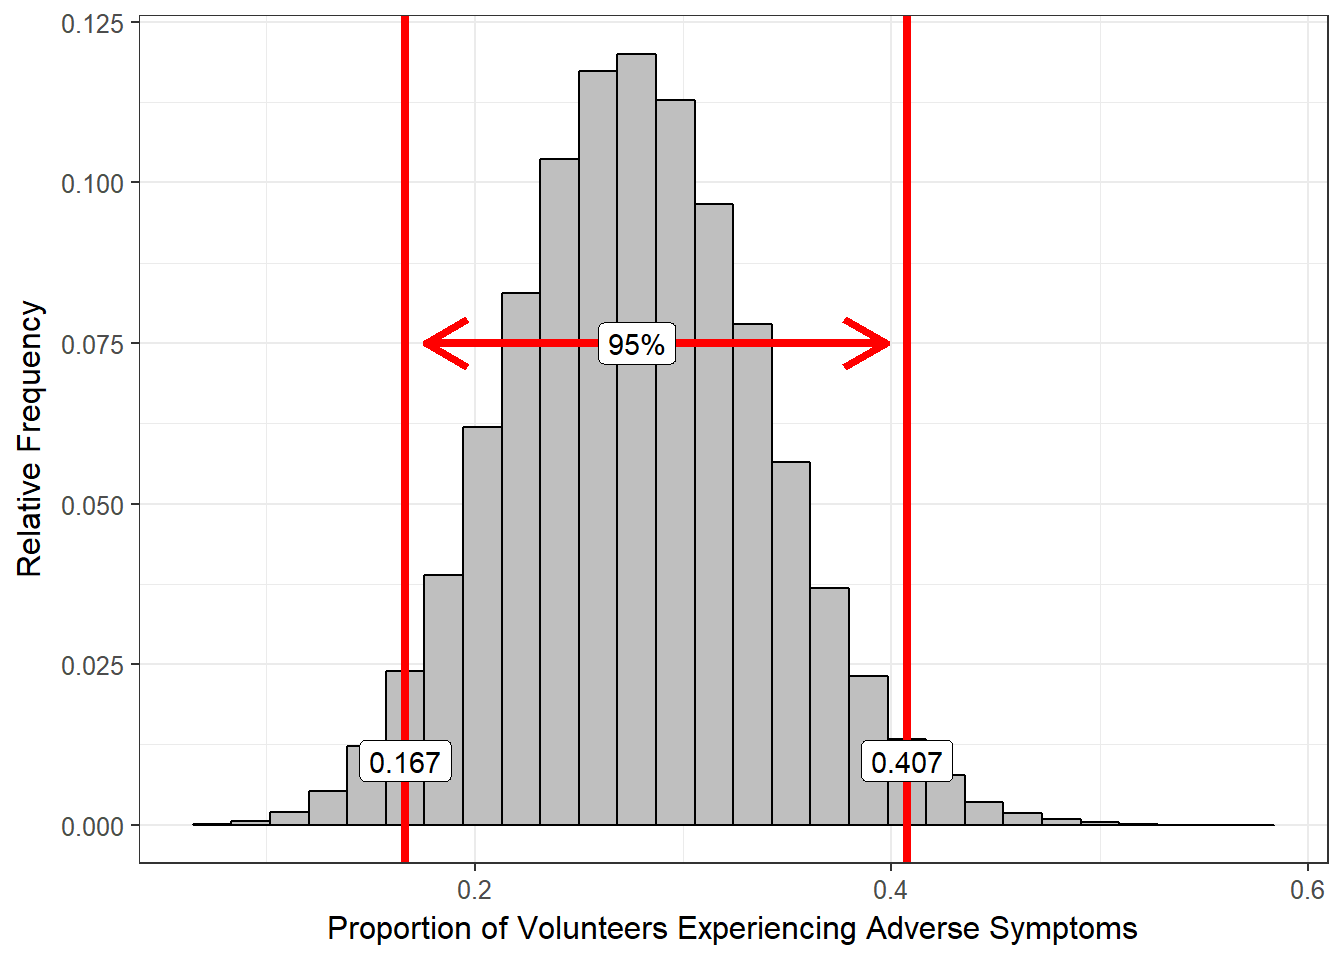
\includegraphics[width=0.8\linewidth]{./Images/samplingdistns-deepwater-95ci-1}

\}

\textbackslash{}caption\{Construction of a 95\% confidence interval via
bootstrapping for the proportion of volunteers assigned to wildlife who
will develop adverse symptoms based on a sample of 54
volunteers.\}\label{fig:samplingdistns-deepwater-95ci}
\textbackslash{}end\{figure\}

Confidence intervals are often misinterpreted; this comes from their
dependence on repeated sampling. When thinking about confidence
intervals, think about playing a game of ring toss: you toss a ring in
hopes of landing on top of a target. The target is the parameter
characterizing the population. The confidence interval is like a ring.
Since the confidence interval is constructed from a model of the
sampling distribution, it changes with each sample; that is, the
confidence interval itself is a statistic. Just like in ring toss, the
ring moves with each toss, the confidence interval moves with each
sample. However, the target stays fixed. Because of this, the following
interpretations are \emph{incorrect}:

\begin{itemize}
\tightlist
\item
  There is a 95\% chance that the proportion of volunteers assigned to
  clean wildlife who will experience adverse symptoms is between 0.167
  and 0.407.
\item
  95\% of volunteers assigned to clean wildlife in our sample had a
  value between 0.167 and 0.407.
\end{itemize}

The first statement is incorrect because it treats the parameter as the
thing that is moving. Once the data has been collected, the confidence
interval is a fixed quantity; neither the estimate or the parameter is
moving; so, there is no probability left. Again, think about tossing a
ring; once the ring is tossed, you either captured the target or you did
not. There is no ``I captured the target with 95\% probability.''

The second statement is absurd in this case. A volunteer either had
respiratory symptoms or they did not; so, saying they had a value
between 0.167 and 0.407 is ridiculous. However, this is a common
misconception with confidence intervals. They are describing reasonable
values of the parameter, not values of the variable in the sample or
population. We recommend sticking to interpreting a confidence interval
as specifying reasonable values for the parameter.

\BeginKnitrBlock{rmdtip}
Confidence intervals \emph{do not} provide a probability that the
parameter is inside. Nor do they tell you anything about the individual
values in a sample or population. They describe reasonable values of the
parameter.
\EndKnitrBlock{rmdtip}

\BeginKnitrBlock{rmdkeyidea}
Confidence intervals specify \emph{reaonable} values of the parameter
based on the data observed.
\EndKnitrBlock{rmdkeyidea}

This is a difficult concept to wrap our heads around; it seems natural
to associate the percentage with the values we have obtained. However,
our confidence is in the \emph{process}, not the resulting interval
itself. That is, a 95\% confidence intervals work 95\% of the time;
however, this statement is about the process of constructing confidence
intervals. Once we have computed a convidence interval, it either has
worked or not; the problem is of course, that since we do not know the
parameter, we will never know if it worked or not. For this reason, we
prefer the interpretation of a confidence interval which avoids these
subtleties: a confidence interval specifies the reasonable values of the
parameter. The percentage (95\% vs 99\% for example) then just specifies
what we mean by ``reasonable.''

It may seem like a good idea to make a 100\% confidence interval to be
sure we always capture the parameter. But, such intervals are not
helpful in practice. For example, a 100\% confidence interval for the
proportion of volunteers experiencing adverse symptoms would be (0, 1).
But, this is useless; it essentially says that the proportion has to be
a number between 0 and 1, but we already knew that. Therefore, we must
balance the confidence we desire with the amount of information the
interval conveys.

\BeginKnitrBlock{rmdtip}
If you want both a high level of confidence but also a narrow interval,
increase the sample size. As the sample size increases, the variability
in the statistic decreases leading to a narrower interval.
\EndKnitrBlock{rmdtip}

\BeginKnitrBlock{rmdtip}
95\% confidence intervals are the most common in practice; however,
90\%, 98\%, and 99\% intervals are also used. It is extremely rare to
use less than a 90\% CI.
\EndKnitrBlock{rmdtip}

\section{Bringing it All Together}\label{bringing-it-all-together}

Consider the following question:

\begin{quote}
Is there evidence that more than 1 in 5 volunteers assigned to clean
wildlife will develop adverse respiratory symptoms?
\end{quote}

Let's answer this question using a confidence interval. Based on the
data obtained, we found that the 95\% confidence interval (CI) for the
proportion of volunteers experiencing adverse symptoms to be (0.167,
0.407). Is this data consistent with more than 1 in 5 volunteers
developing adverse symptoms? Yes, since there are proportions within
this interval which are larger than 0.2. But, \emph{consistency} is not
the same as \emph{evidence}; remember, evidence is the idea of ``beyond
a reasonable doubt.'' After all, is this data \emph{consistent} with
less than 1 in 5 volunteers developing adverse symptoms? Yes, since
there are proportions within this interval which are less than 0.2.

Confidence intervals specify reasonable values --- those values of the
parameter which are consistent with the data. This data is then
consistent with proportions that are both less than 0.2 and greater than
0.2. So, what can we say then? We can say that there is \emph{not}
evidence that more than 1 in 5 volunteers assigned to clean wildlife
will develop adverse respiratory symptoms, but the data is consistent
with this claim.

More, we can say that there \emph{is evidence} that the proportion of
volunteers who will develop symptoms is less than 0.5; further, the
proportion of volunteers who will develop symptoms is larger than 0.1.
That is, the data provides evidence that more than 10\% of volunteers
will develop adverse symptoms, but this percentage will not be larger
than 50\%. How do we know? Because values less than 10\% are not
reasonble values of the parameter based on the 95\% CI. Values like 0.1
are outside of the confidence interval and are therefore not reasonable.
Similarly, values above 0.5 are outside the confidence interval and are
therefore not reasonable.

The power of a model for the sampling distribution is that it allows us
to determine which values of a parameter are reasonable and which values
are not.

\chapter{Quantifying the Evidence (Rejecting Bad
Models)}\label{NullDistns}

Again, the goal of statistical inference is to use the sample as a
snapshot of the underlying population (Figure
\ref{fig:nulldistns-statistical-process}). Recall that there are
essentially two categories of questions we ask when trying to perform
inference:

\begin{itemize}
\tightlist
\item
  Estimation: what \emph{proportion} of volunteers who clean wildlife
  following an oil spill will experience adverse respiratory symptoms?
\item
  Model Consistency: is it reasonable that no more than 1 in 5
  volunteers who clean wildlife following an oil spill will experience
  adverse respiratory symptoms?
\end{itemize}

\begin{figure}

{\centering 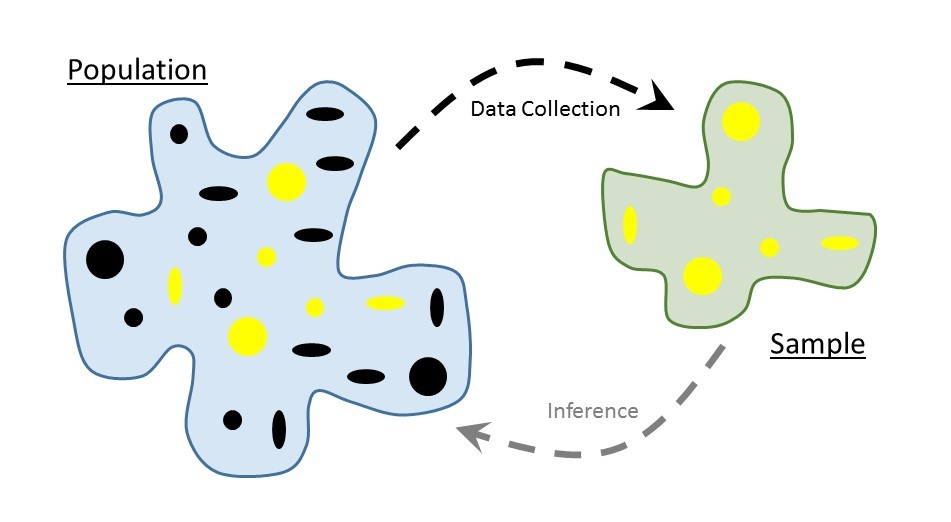
\includegraphics[width=0.8\linewidth]{images/Basics-Stat-Process} 

}

\caption{Illustration of the statistical process (reprinted from Chapter 1).}\label{fig:nulldistns-statistical-process}
\end{figure}

In the previous chapter we addressed these questions through the use of
confidence intervals --- by specifying reasonable values of the
parameters through a model of the sampling distribution. However, when
working with questions of the second type (model consistency), there is
a second approach; this latter approach is useful when confidence
intervals cannot be constructed for the particular question of interest
(see Unit 2).

Remember, assessing model consistency is similar to performing a trial
in a court of law. After gathering the evidence, the jury is left with
the following decision:

\begin{itemize}
\tightlist
\item
  Assuming the defendant is innocent, if the evidence is unlikely to
  have occurred (so is not consistent with innocence), then they vote
  ``guilty.''
\item
  Assuming the defendant is innocent, if the evidence is reasonably
  likely to have occurred (so is consistent with innocence), then they
  vote ``not guilty.''
\end{itemize}

The goal in this section is to somehow quantify the evidence against a
particular model to determine if we can say that the data is not
consistent with the given model.

\section{Some Subtleties}\label{some-subtleties}

In a U.S. trial, there are some subtleties that we should be aware of,
as they also creep up in statistical analyses and have implications for
how we interpret statistical results. First, the jury weighs the
evidence \emph{under the assumption of innocence}. That is, they first
develop a working hypothesis (the defendant is innocent). Then, the
likelihood of the evidence \emph{under this assumption} is determined.
For example, if a defendant were innocent of murder, it is unlikely to
have five eye witnesses stating the defendant was seen standing over the
victim, holding the murder weapon, and screaming ``I killed him!'' Since
that evidence does not jive with innocence, the jury convicts. If,
however, the only evidence is that five eye witnesses place the
defendant in the same city as the victim and the defendant matches the
description of someone seen fleeing the crime scene, then the jury would
not convict. Why? Because the evidence, while pointing toward guilt, is
not overwhelming; these things could have happened by chance alone.
Therefore, the evidence, while consistent with guilt does not provide
evidence for guilt.

Also notice that a jury saying ``not guilty'' is not the same as saying
``innocent.'' That is, a lack of evidence to convict does not imply the
defendant is innocent. A lack of evidence is simply a lack of evidence.
The defendant may still be guilty, but the evidence has just not proven
it.

Similarly, when assessing model consistency, we will weigh the data
\emph{under the null hypothesis} (our working assumption). Then, the
likelihood of our data occurring by chance alone \emph{under this
hypothesis} is determined. If that likelihood is small (data is not
consistent with the null hypothesis), we can conclude the data supports
the alternative hypothesis (guilty). If, however, that likelihood is
large (data is consistent with the null hypothesis), we can only
conclude that the data is consistent with the hypotheses. We are
\emph{not} able to say ``supports the null'' because that would be like
saying a defendant is innocent. We can't prove innocence because we
started by assuming it!

\section{Assuming the Null
Hypothesis}\label{assuming-the-null-hypothesis}

Consider the question we have been asking regarding the
\protect\hyperlink{CaseDeepwater}{Deepwater Horizon Case Study}:

\begin{quote}
Is there evidence that more than 1 in 5 volunteers assigned to clean
wildlife will develop adverse respiratory conditions?
\end{quote}

Remember, we framed this question through statements about a parameter
in Chapter \ref{Questions}:

\begin{quote}
\(H_0:\) the proportion of volunteers assigned to clean wildlife who
develop adverse respiratory symptoms is no more than 0.20.\\
\(H_1:\) the proportion of volunteers assigned to clean wildlife who
develop adverse respiratory symptoms exceeds 0.20.
\end{quote}

Within the sample we observed that 27.8\% of volunteers experienced
adverse symptoms, which is certainly more than the 0.20 in the claim;
therefore, the data is at least trending toward the alternative
hypothesis. However, it is possible that we just have a strange sample.
Remember in our discussion of sampling distributions in the previous
chapter, however, that we expect the estimate to vary from one sample to
another. Essentially, we need to know whether 27.8\% of volunteers
experiencing symptoms is a strong signal that the rate within the
popoulation is larger than 0.2 (1 in 5) or 27.8\% is simply a fluke that
might happen due to sampling variability. While we are going to be
attacking the question differently in this chapter than the previous, we
see that the key is still variability in the estimate. That is, we are
back to the \emph{Fourth Fundamental Idea of Inference}. As stated
above, in order to determine evidence for one statement (captured by the
alternative hypothesis), we begin by assuming the opposite statement
(captured by the null hypothesis) as our working assumption. That is, if
we want to know if 27.8\% of volunteers experiencing adverse symptoms is
``evidence,'' we need to figure out what we \emph{expect} to happen
\emph{if only 1 in 5 volunteers actually develop adverse respiratory
symptoms}.

Consider this last statement. It is equivalent to saying ``what type of
evidence would we expect for an innocent person?'' Only if we know what
to expect can we determine if the evidence in front of us is extreme
enough to convict. Only if we know what to expect can we determine if
the observed sample provides evidence in favor of the alternative. So,
we enter a fake world\ldots{}a world in which exactly 1 in 5 volunteers
actually develop respiratory symptoms. That is, we enter a world in
which the null hypothesis is true. Now, in this world, how do we know
what to expect? We construct the sampling distribution for the
proportion under this assumption that the null hypothesis is true; this
is known as the \textbf{null distribution}.

\BeginKnitrBlock{definition}[Null Distribution]
\protect\hypertarget{def:defn-null-distribution}{}{\label{def:defn-null-distribution}
\iffalse (Null Distribution) \fi{} }The sampling distribution of a
statistic \emph{if} the null hypothesis is true.
\EndKnitrBlock{definition}

To construct the null distribution, we do the following steps
(illustrated in Figure \ref{fig:nulldistns-null-distribution}:

\begin{enumerate}
\def\labelenumi{\arabic{enumi}.}
\tightlist
\item
  Sample randomly from a fake population where the null hypothesis is
  true.
\item
  For each sample, compute the statistic of interest.
\item
  Repeat steps 1 and 2 several thousand times.
\item
  Plot the statistics retained from each sample.
\end{enumerate}

\begin{figure}

{\centering 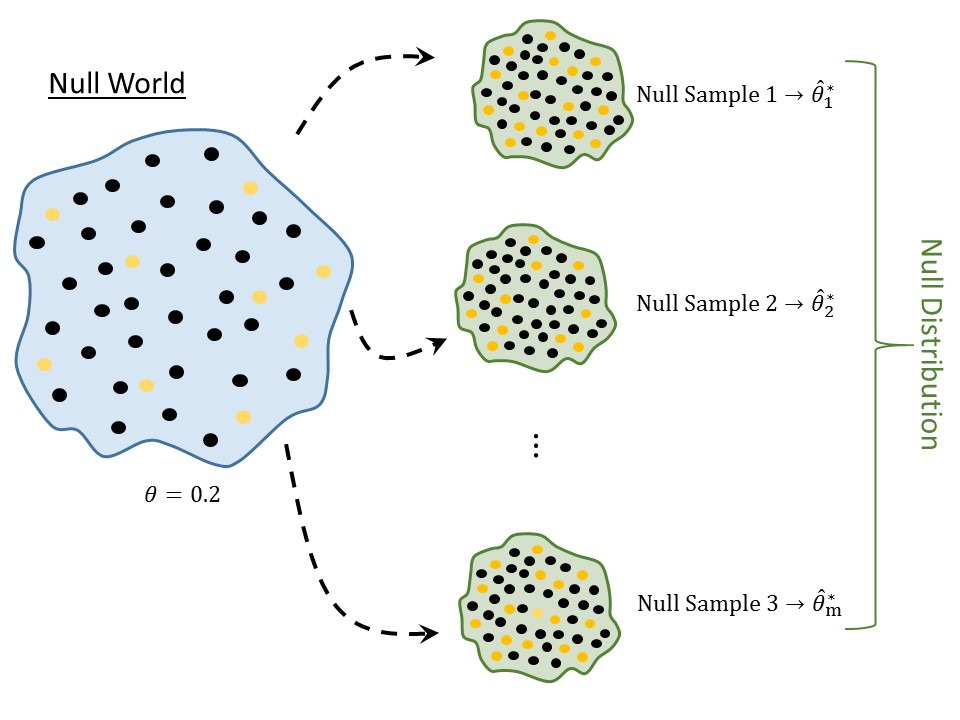
\includegraphics[width=0.8\linewidth]{./images/NullDistns-Null-Distribution} 

}

\caption{Illustration of constructing a null distribution.  Notice the similarity to constructing the sampling distributon.}\label{fig:nulldistns-null-distribution}
\end{figure}

Notice that these are the same steps as in constructing a sampling
distribution with the exception that instead of sampling from the
population of interest, we sample from a hypothetical population in
which the null distribution is true. With today's computational power,
we are able to make such samples possible similar to bootstrapping since
we can make the null population in a virtual world and sample from it.
That is, we are simulating what would happen if the null hypothesis were
true. Figure \ref{fig:nulldistns-deepwater-null} represents the null
distribution for the proportion of volunteers in a sample of 54 assigned
to clean wildlife which would develop adverse sympoms when the null
hypothesis is that the proportion is 0.20.

\begin{figure}

{\centering 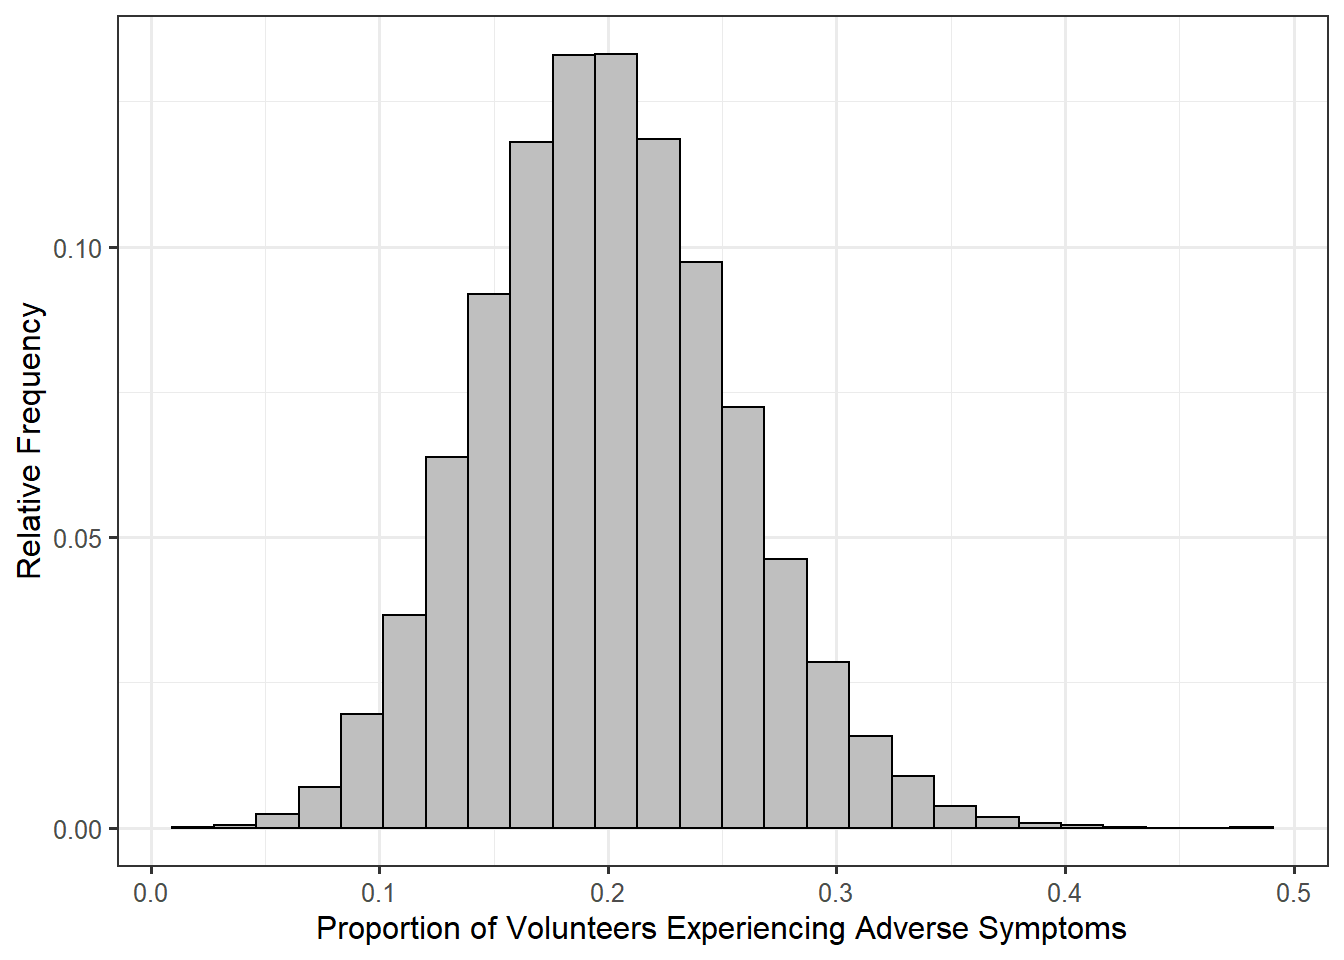
\includegraphics[width=0.8\linewidth]{./Images/nulldistns-deepwater-null-1} 

}

\caption{Null distribution for the proportion of volunteers assigned to clean wildlife experiencing adverse respiratory symptoms.  Null hypothesis is that the proportion is 0.20; this is based on a sample of size 54.}\label{fig:nulldistns-deepwater-null}
\end{figure}

\section{Using the Null Distribution}\label{using-the-null-distribution}

From the figure, we see that \emph{if the null hypothesis were true} ---
if only 1 in 5 volunteers assigned to clean wildlife experienced
symptoms --- then in a sample of 54 individuals, we would expect the
proportion who experienced symptoms to be somewhere between 0.1 and 0.3.
\emph{If the null hypothesis were true}, it would be nearly impossible
that half of the individuals experienced symptoms (since 0.5 is way off
in the tail of the distribution). The further in the tail region, the
more extreme the sample. The question is then how extreme is our sample?
Again, the null distribution is just setting up expectations; now, we
have to weigh the evidence against those expectations.

In our sample, we observed 27.8\% of volunteers who experienced
symptoms. Since 0.278 is towards the center of the distribution, we
would say that it is not an extreme sample. In order to quantify how
extreme (or not extreme) its, we find out what fraction of values are
more extreme (larger than in this case) than the value observed; that
is, what fraction of values appear in the right tail of the
distribution. Figure \ref{fig:nulldistns-deepwater-pvalue} illustrates
this computation. Based on the null distribution, there is a 10.6\%
chance that \emph{if the null hypothesis were true} --- only 1 in 5
volunteers actually experienced symptoms --- that in a random sample of
54 volunteers we would obtain data this extreme or moreso by chance
alone. Essentially, this tail area is quantifying the strength of the
evidence. The smaller this area, the further in the tail region our data
is; that is, our data is more unexpected. Therefore, small areas
indicate that the data (our evidence) does not jive with our
expectations under the null (innocence), forcing us to conclude the data
provides evidence \emph{against} the null hypothesis. In our case, since
the area is relatively large, our data is completely consistent with
what we might expect if the null were true. Therefore, in this case, we
conclude that there is no evidence that the rate of those experiencing
symptoms exceeds 1 in 5. This area is known as the \textbf{p-value}.

\begin{figure}

{\centering 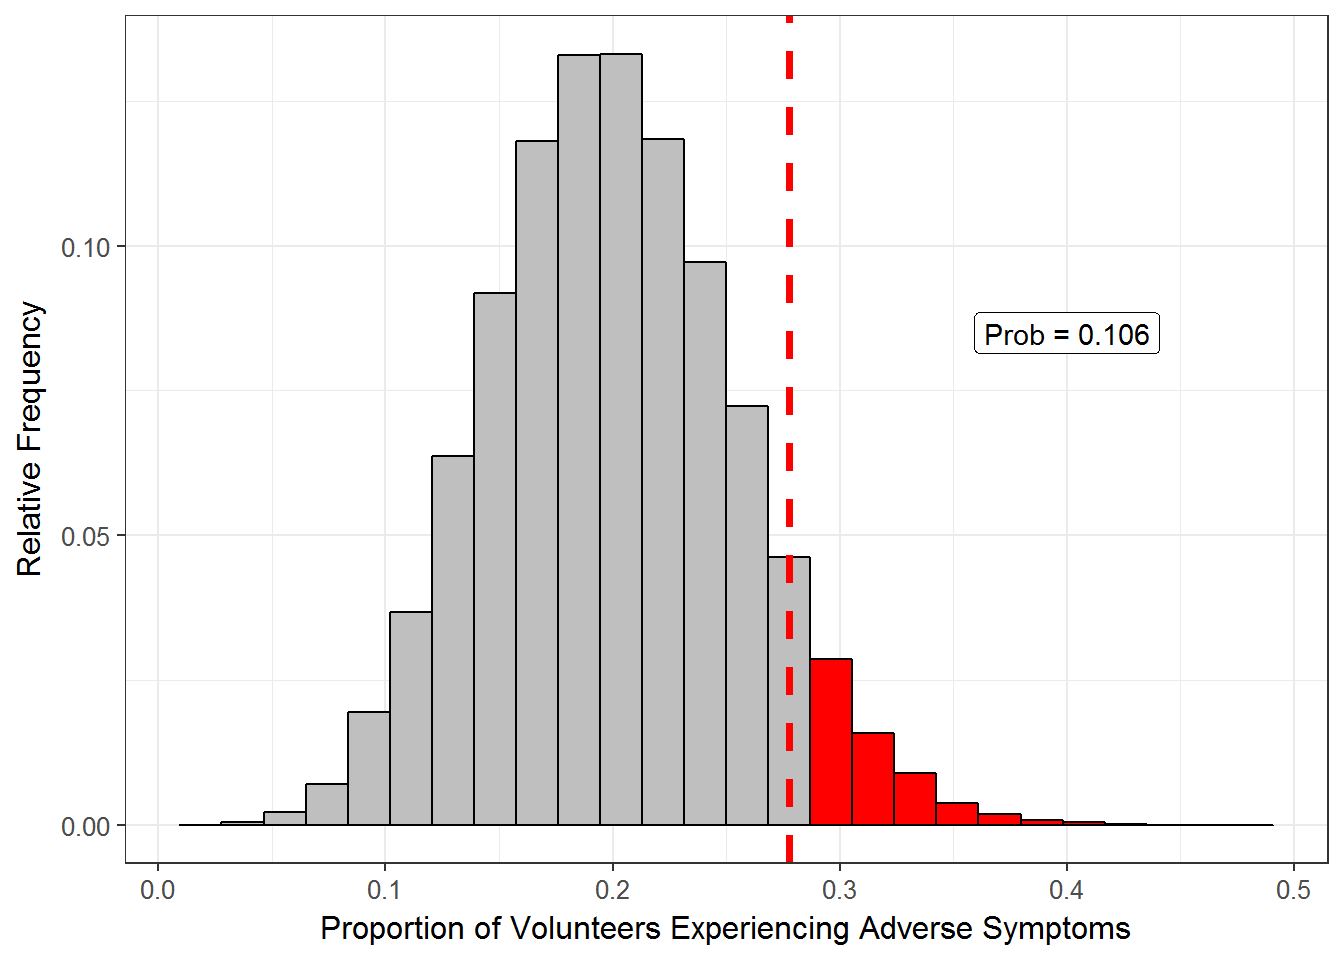
\includegraphics[width=0.8\linewidth]{./Images/nulldistns-deepwater-pvalue-1} 

}

\caption{Likelihood of obtaining a sample as extreme or moreso as that of the original sample when the parameter of interest is the proportion of volunteers assigned to clean wildlife experiencing adverse respiratory symptoms.  Null hypothesis is that the proportion is 0.20; this is based on a sample of size 54.}\label{fig:nulldistns-deepwater-pvalue}
\end{figure}

\BeginKnitrBlock{definition}[P-Value]
\protect\hypertarget{def:defn-pvalue}{}{\label{def:defn-pvalue}
\iffalse (P-Value) \fi{} }The probability, assuming the null hypothesis
is true, that we would observe a statistic, by chance alone, as extreme
or moreso as that observed in our sample. This quantifies the strength
of evidence against the null hypothesis. Smaller values indicate
stronger evidence.
\EndKnitrBlock{definition}

It is natural to ask ``how small does the p-value need to be to prove a
statement?'' Like a trial, the weight of the evidence presented depends
on the context. In some studies, a p-value less than 0.01 may be strong
evidence while in other studies a p-value less than \(10^{-6}\) is
required. And, as in a trial, it is not only the strength of the
evidence but the type of evidence presented (DNA evidence may be
stronger than fingerprint evidence). In statistics, it is important to
consider the effect size as well as the p-value. That is, consider
whether the difference between the estimate and the null value is
actually large; this is always based on subject-matter expertise. It is
often helpful to report a confidence interval alongside a p-value.

\BeginKnitrBlock{rmdtip}
While what constitutes ``significant'' may vary from discipline to
discipline, the list below is a good rule of thumb:

\begin{itemize}
\tightlist
\item
  \(p \geq 0.1\): no evidence against the null hypothesis.
\item
  \(0.05 \leq p < 0.1\): weak evidence against the null hypothesis.
\item
  \(0.01 \leq p < 0.05\): some evidence against the null hypothesis.
\item
  \(0.001 \leq p < 0.01\): evidence against the null hypothesis.
\item
  \(p < 0.001\): strong evidence against the null hypothesis.
\end{itemize}

As with any rule of thumb, this should not be considered binding and may
vary depending on the application.
\EndKnitrBlock{rmdtip}

Like confidence intervals, p-values are often misinterpreted. In fact,
they have become so abused that some researchers argue against their
use. It is our opinion that the p-value can be a useful tool once it is
appropriately understood; so, let's dispell some of these
misconceptions. Consider these \emph{incorrect} statements regarding the
p-value obtained for the \protect\hyperlink{CaseDeepwater}{Deewater
Horizon Case Study} computed above:

\begin{itemize}
\tightlist
\item
  There is a 10.6\% chance that only 1 in 5 volunteers assigned to clean
  wildlife will experience adverse symptoms.
\item
  Since the p-value is large, there is evidence (or the data supports
  the claim) that 1 in 5 volunteers assigned to clean wildlife will
  experience adverse symptoms.
\end{itemize}

The first statement incorrectly assumes that there is some chance that
the null hypothesis is true. Remember, our two hypotheses are statements
about the parameter. One is true and other is not. Our ignorance does
not change this; therefore, it does not make sense to talk about the
probability of the null being true or false. Instead, our job is to
quantify the likelihood of the data \emph{assuming the null is true}.
The p-value is about the likelihood of the data under a particular model
(the null hypothesis).

The second statement makes the common mistake that a lack of evidence
for the alternative is evidence in favor of the null. A lack of evidence
is like a ``not guilty'' verdict. It simply means we were not convinced.
However, it does not mean that the defendant is innocent. All we are
saying with the large p-value in this case is that the data is
\emph{consistent} with only 1 in 5 volunteers getting adverse symptoms;
unfortunately, it is also \emph{consistent} with more than 1 in 5
volunteers getting adverse symptoms. This may be an unsatisfying
conclusion, but it is still a conclusion nonetheless. Our conclusion was
based on assessing the variability of a the statistic under a particular
model. This is captured in our last of the \emph{Five Fundamental Ideas
of Inference}:

\BeginKnitrBlock{rmdfivefund}
\textbf{Fundamental Idea V}: With a model for the distribution of a
statistic, we can quantify the error in our estimate and the likelihood
of a sample under a proposed model. This allows us to draw conclusions
about the corresponding parameter, and therefore the population, of
interest.
\EndKnitrBlock{rmdfivefund}

\section{Sampling Distributions vs.~Null
Distributions}\label{sampling-distributions-vs.null-distributions}

Clearly the sampling distribution and null distribution of a statistic
are closely related. The difference is that the null distribution is
created under a proposed model while the sampling distribution lets the
data speak for itself. It is worth taking just a moment to highlight the
differences in the use of these two components of the
\emph{Distributional Quartet}.

The sampling distribution is centered on the true value of the
parameter; the null distribution is centered on the null value. Once we
assume the null hypothesis is true, we have a value for the parameter;
as a result, we expect the sampling distribution under this assumption
(that is, the null distribution) to be centered on this hypothesized
value. So, null distributions are \emph{always} centered on the null
value.

Sampling distributions lead to confidence intervals by specifying
reasonable values of the parameter.

Null distributions lead to p-values by quantifying the likelihood of our
data under a proposed model.

\BeginKnitrBlock{rmdtip}
Model the sampling distribution to construct a confidence interval; to
assess a hypothesis the null value is overlayed on the sampling
distribution. Extreme values of the distribution are unreasonable values
for the parameter.

Model the null distribution to compute a p-value; to assess a
hypothesis, the statistic from the sample is overlayed on the null
distribution. Extreme values of the distribution are values which
provide evidence against the null hypothesis.
\EndKnitrBlock{rmdtip}

\chapter{Using the Tools Together}\label{RecapLanguage}

In this unit, we have introduced the key components in both the language
and logic of statistical inference. In fact, with a firm grasp of the
concepts in this unit, you should be able to read and interpret key
statistical findings. All statistical analyses make use of the
\emph{Five Fundamental Ideas of Inference} and alternate between the
members of the \emph{Distributional Quartet}. The context of each
problem differs, but the logic remains the same. In this chapter, we
present another analysis based on the
\protect\hyperlink{CaseDeepwater}{Deepwater Horizon Case Study},
annotating it along the way to see how these elements work together
fluidly to reach a conclusion. Specifically, we are interested in the
following question:

\begin{quote}
Are volunteers assigned to clean wildlife at higher risk of developing
adverse respiratory symptoms compared to those volunteers who do not
come into direct contact with oil? If so, estimate the increased risk.
\end{quote}

\section{Framing the Question (Fundamental Idea
I)}\label{framing-the-question-fundamental-idea-i}

We are really interested in whether the rate of respiratory symptoms in
one group of volunteers is larger than that in a second group.
Therefore, our working assumption is that there is no difference in the
rate of respiratory symptoms between these two groups. That is, we have

\begin{quote}
\(H_0:\) the rate of adverse respiratory symptoms is similar between
volunteers assigned to clean wildlife and those assigned to tasks which
do not involve direct exposure to oil.\\
\(H_1:\) the rate of adverse respiratory symptoms is greater for
volunteers assigned to clean wildlife and those assigned to tasks which
do not involve direct exposure to oil.
\end{quote}

We can also state this more formally with mathematical notation as
follows:

\begin{quote}
Let \(\theta_1\) be the rate of developing adverse respiratory symptoms
for volunteers assigned to clean wildlife.\\
Let \(\theta_2\) be the rate of developing adverse respiratory symptoms
for volunteers assigned to tasks without direct exposure to oil.\\
\(H_0: \theta_1/\theta_2 \leq 1\)\\
\(H_1: \theta_1/\theta_2 > 1\)
\end{quote}

The ratio \(\theta_1/\theta_2\) is known as the \emph{risk ratio} as it
captures the increased risk for one group compared to another.

Notice that this is a well-posed question as it centers on parameters
which characterize the population. Therefore, it can be answered with
appropriate data.

\begin{quote}
Distribution of the Population: Our questions of interest are about the
population and therefore focus on characterizing this distribution.
\end{quote}

\section{Getting Good Data (Fundamental Idea
II)}\label{getting-good-data-fundamental-idea-ii}

As we are working with previously collected data, we are unable to
design a good sampling scheme. The only thing we can do at this point is
critique the sample we have. The key question to ask ourselves is
whether there is any reason that these group of volunteers differs
systematically from other volunteers working oil spills. For example,
this oil spill occurred in the Gulf of Mexico; the majority of
volunteers were then naturally residents of Gulf states. It is possible
that these residents are somehow fundamentally different with respect to
their risk of developing adverse respiratory symptoms compared to the
remainder of the United States. If that is the case, the results of this
study would not generalize to oil spills occuring in the Atlantic.
However, it is probably reasonable to say that these results would apply
to future oil spills in the Gulf.

Also note that this was not a controlled experiment. Volunteers were not
randomly allocated to their assignments that we know of. Therefore, our
results could be somewhat limited. The two groups should be compared
regarding other attributes (this data is unavailable to us currently) in
order to determine if they are similar with respect to other variables
which may potentially confound the results.

\section{Presenting the Data (Fundamental Idea
III)}\label{presenting-the-data-fundamental-idea-iii}

The heart of this question is comparing the rate of adverse events in
each group. Figure \ref{fig:recaplanguage-deepwater-plot} makes this
comparison.

\begin{figure}

{\centering 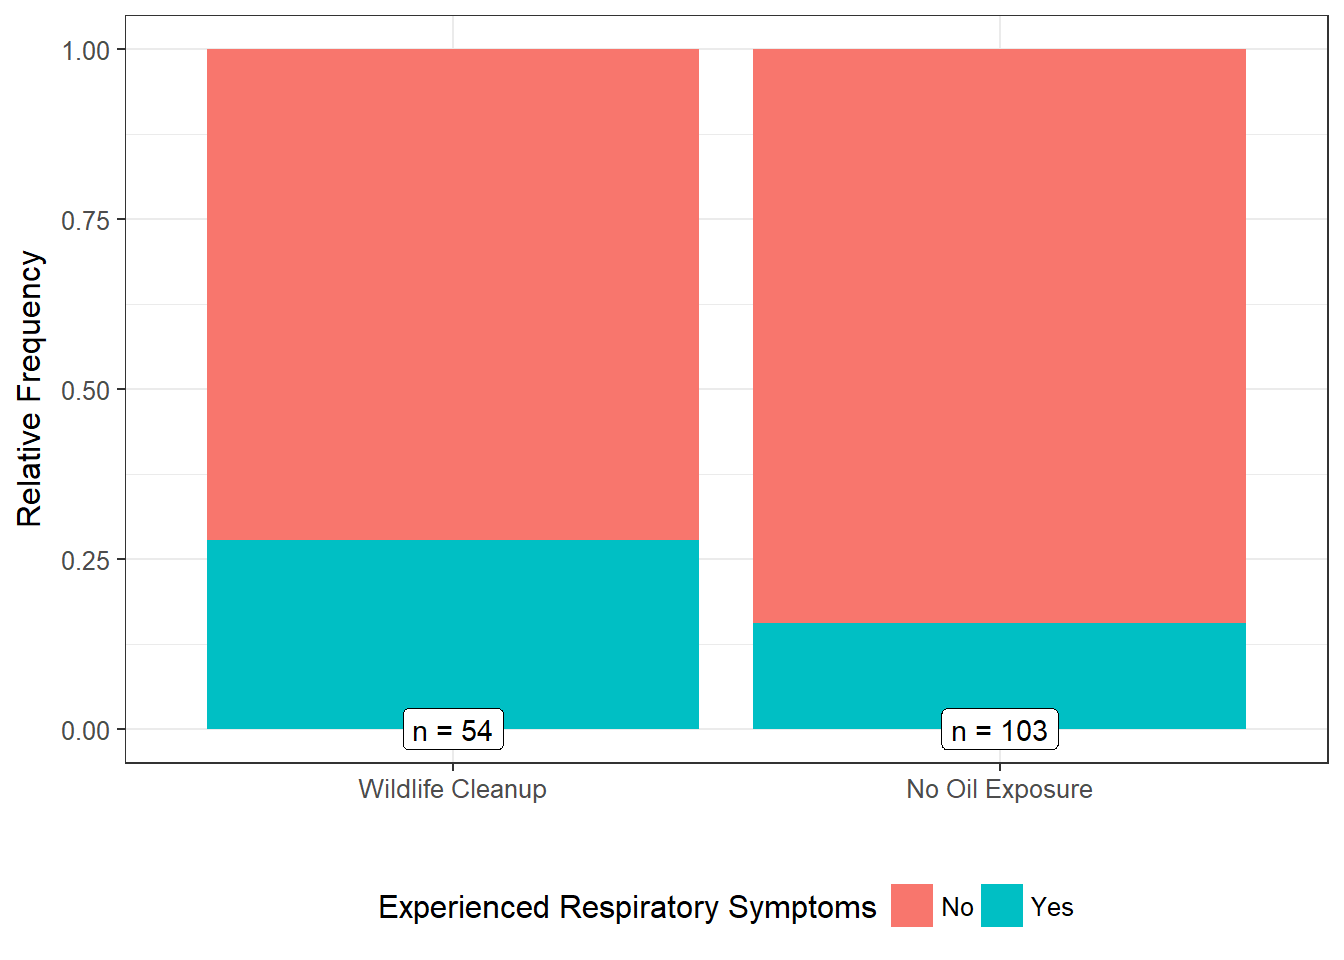
\includegraphics[width=0.8\linewidth]{./Images/recaplanguage-deepwater-plot-1} 

}

\caption{The risk of developing adverse respiratory symptoms for volunteers assigned to clean wildlife and those volunteers assigned to tasks which do not have direct exposure to oil.}\label{fig:recaplanguage-deepwater-plot}
\end{figure}

As seen in the figure, the rate of adverse respiratory symptoms is
larger in the group of volunteers assigned to wildlife cleanup. The rate
of respiratory symptoms is 1.79 times higher in the volunteers assigned
to clean wildlife compared to those assigned to tasks with no direct oil
exposure.

Notice that we reported the relative risk comparing the two groups as it
is directly tied to how we specified the hypotheses above.

\begin{quote}
Distribution of the Sample: graphics and numerical summaries
characterize this distribution, informing us about the underlying
population. This is possible as long as the sample is representative of
the population.
\end{quote}

\section{Quantifying the Variability in the Estimate (Fundamental Idea
IV)}\label{quantifying-the-variability-in-the-estimate-fundamental-idea-iv}

While we have an estimate for the increased risk of adverse respiratory
symptoms for those volunteers assigned to clean wildlife, the estimate
has not taken into account the variability in the sample. In order to
quantify this variability, we use a bootstrap procedure to model the
sampling distribution of the risk ratio. Observe that we focus on the
sampling distribution of the statistic that estimates the parameter of
interest.

Recall that the bootstrap mimics the process for generating a sampling
distribution. In this case, ``repeating the study'' involves collecting
data from not one, but two groups. So, we must resample both from the 54
volunteers who were assigned to clean wildlife and the 103 volunteers
assigned to tasks not involving direct oil exposure. Each time we
resample, we ensure that we select 54 volunteers who clean wildlife and
103 who do not. We need the process of the original study to be
maintained. Each time we resample from these groups, we compue the
relative risk and retain this value. Figure
\ref{fig:recaplanguage-sampling-distribution} shows the sampling
distribution for the relative risk comparing these two groups. Again, it
is important to note that we are not generating \emph{new} data; we are
\emph{resampling}/\emph{reusing} the original sample.

\begin{figure}

{\centering 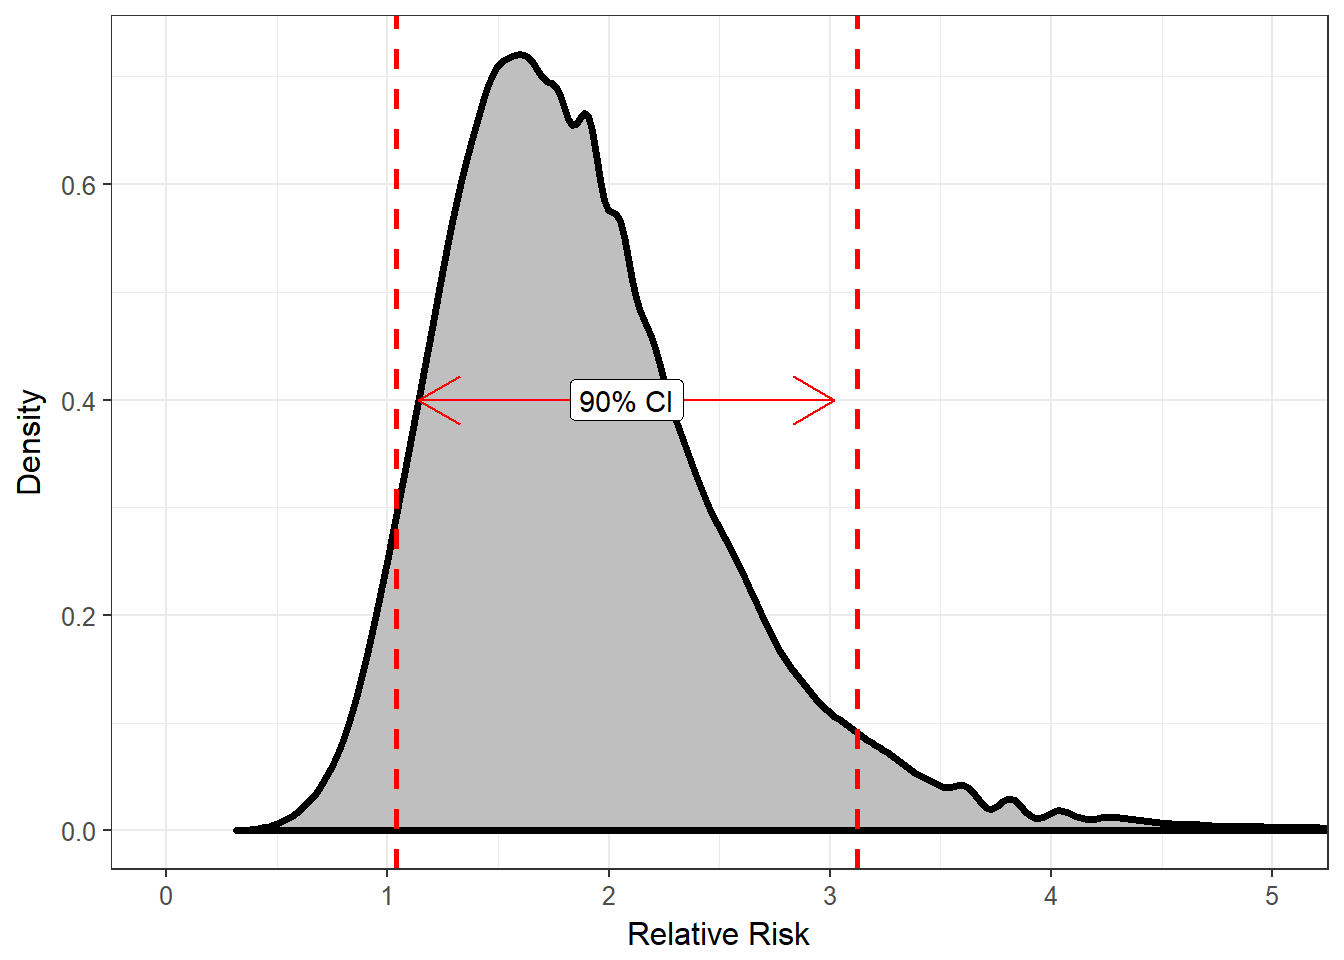
\includegraphics[width=0.8\linewidth]{./Images/recaplanguage-sampling-distribution-1} 

}

\caption{Model of the sampling distribution for the relative risk comparing volunteers assigned to clean wildlife to volunteers assigned to tasks not involving oil exposure.  The model was developed via bootstrapping using 50000 replications.}\label{fig:recaplanguage-sampling-distribution}
\end{figure}

Volunteers assigned to clean wildlife have are 1.79 times (95\% CI =
(0.92, 3.47)) more likely to experience adverse respiratory symptoms
compared to those volunteers assigned to tasks not requiring direct
exposure to oil. Our data suggests that our data is consistent with the
two groups having a similar risk but tends toward volunteers assigned to
clean wildlife being at increased risk..

\begin{quote}
Sampling Distribution: allows us to quantify the variability in the
statistic and provide an interval estimate for the paraemter which
incorporates this variability.
\end{quote}

\section{Quantifying the Evidence (Fundamental Idea
V)}\label{quantifying-the-evidence-fundamental-idea-v}

In order to quantify the departure of the data from our working
assumption that the risk is similar between the two groups, we rely on
the null distribution and compute a p-value.

\begin{figure}

{\centering 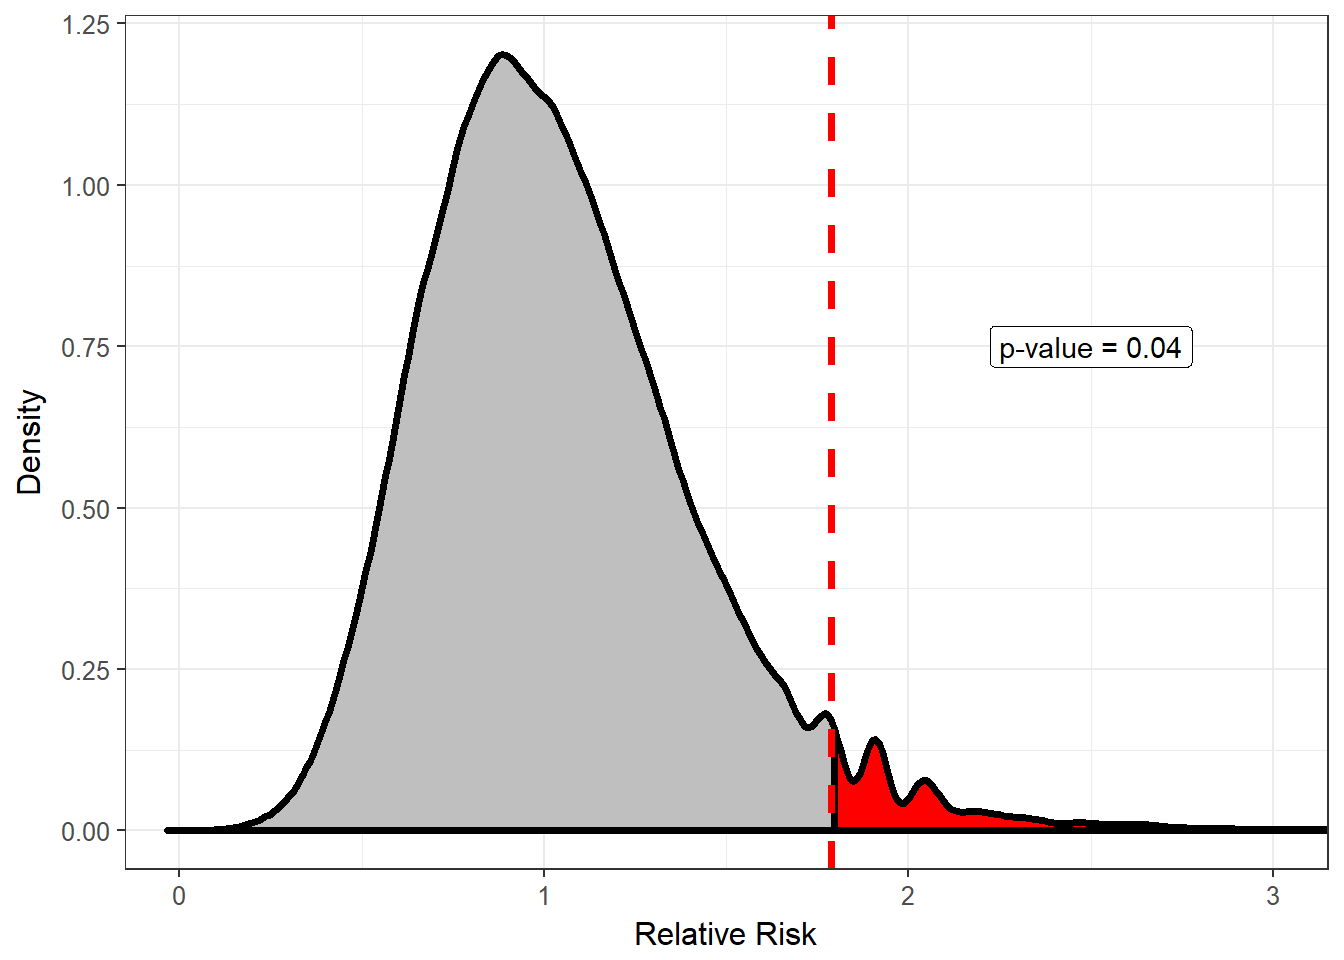
\includegraphics[width=0.8\linewidth]{./Images/recaplanguage-null-distribution-1} 

}

\caption{Null distribution for the relative risk comparing volunteers assigned to clean wildlife to volunteers assigned to tasks not involving oil exposure.  The null hypothesis assumed the two groups of volunteers had a similar risk.  The nul distribution was developed via bootstrapping using 50000 replications.}\label{fig:recaplanguage-null-distribution}
\end{figure}

There is some evidence (p = 0.04) to suggest that volunteers exposed to
oil have an increased risk of developing adverse respiratory symptoms.
Given the estimated level of this increased risk, we believe this is
something health officials should investigate further. It would be worth
investigating further what aspects of the oil exposure may have caused
the increased risk to determine if it can be avoided in the future.

Note we are careful to not claim that the assignments have caused an
increase in the risk as this data is not from a controlled experiment.
This is one of the limitations of this analysis. However, if we are able
to assume the two groups are fairly similar with respect to other
attributes --- that is, there is no reason why people prone to
respiratory symptoms would become assigned to wildlife cleaning --- then
we may have some reason to believe the results are causal. We will
wrestle more with these types of conclusions in the next unit.

\begin{quote}
Null Distribution: allows us to quantify the level of evidence against a
particular claim; how strongly do the data disagree with the working
assumption.
\end{quote}

\section{Summary}\label{summary}

Notice that our analysis moved through the \emph{Five Fundamental
Ideas}, and in doing so made use or referenced each of the four
components of the \emph{Distributional Quartet}. As we move through the
remainder of the text, we will explore how these frameworks are used in
various other analysis scanarios. As we do, we reveal additional
concepts that underly statistical modeling.

We admit that there are several other questions that may be raised by
the above analysis. This unit is meant to introduce the big concepts of
inference. We will concern ourselves more with the details as we
progress through the text.

\part{Unit II: Comparing the Average Response Across
Groups}\label{part-unit-ii-comparing-the-average-response-across-groups}

\hypertarget{CaseOrganic}{\chapter{Case Study: Organic Foods and
Superior Morals}\label{CaseOrganic}}

``You are what you eat'' is a common phrase dating back to at least the
1820's used to suggest that if you want to be fit, you must eat healthy
foods. However, does the phrase extend to our personality as well as our
physique? Recent research has suggested that specific tastes (sweet
vs.~disgusting, for example) can influence moral processing. That is,
certain foods may lead us to be nicer to those around us or lead us to
be more judgemental. Organic foods are often marketed using phrases like
``pure'' or ``honest'' (Jessica Alba's
\href{https://www.honest.com/}{Honest Company}, for example); is there
some relationship between the consumption of organic foods and moral
behavior?

Dr.~Eskine of the Department of Psychological Sciences at Loyola
University sought to answer this question (Eskine
\protect\hyperlink{ref-Eskine2013}{2013}). He conducted a study to
investigate whether exposure to certain types of food had an effect on a
person's moral processing. Specifically, he randomized 62 Loyola
University undergradates to one of three food types: organic, comfort,
and control. Each participant received a packet containing pictures of
four food items from the assigned category:

\begin{itemize}
\tightlist
\item
  Organic Foods: apple, spinach, tomato, carrot
\item
  Comfort Foods: ice cream, cookie, chocolate, brownie
\item
  Control Foods: oatmeal, rice, mustard, beans
\end{itemize}

The control foods are those which are pre-packaged and are generally
considered staple items; organic foods are those which are associated
with a healthy diet; and, comfort foods were sweets. After viewing the
images for a set period of time, each participant received a packet
containing six counter-balanced moral transgressions. An example of such
a transgression is produced below:

\begin{quote}
Bob was at a family gathering when he met Ellen, a second cousin of his
that he had seen once or twice before. Bob found Ellen very attractive
and he asked her out on a date. Ellen accepted and they began to have a
romantic and sexual relationship. They often go on weekend trips to
romantic hotels in the mountains.
\end{quote}

Participants were then asked to rate the morality of the scenario on a
7-point scale (1 = ``not at all morally wrong'' to 7 = ``very morally
wrong''). The average of the morality scores across the six scenarios
was used as an overall measure of their moral expectations. A higher
value indicates high moral expectations (very strict) and a lower value
indicates lower moral expectations (very lenient).

Dr.~Eskine's analysis revealed that there was strong evidence
(\(p = 0.001\)) that participants' moral judgments differed, on average,
across the various food exposure groups. In particular, those exposed to
organic foods had higher moral expectations (an average mean moral
judgment of 5.58) compared to those experiencing comfort foods (average
mean moral judgment of 4.89) or control foods (average mean moral
judgment of 5.08). He therefore concluded that exposure to organic food
did lead to higher moral expectations.

Understandably, Dr.~Eskine's work caught the interest of various media
outlets and researchers. Two researchers within the Department of
Psychology at Domincan University in Illinois sought to replicate
Dr.~Eskine's work (Moery and Calin-Jageman
\protect\hyperlink{ref-Moery2016}{2016}). There were several components
to their research, but the first phase included a replication of
Dr.~Eskine's initial study with minor variants. They enrolled 124
college students into their study. The participants were presented with
the same food images as in Eskine's study with the exception that celery
was used instead of an apple for organic food. The same moral dilemmas
were given to participants. As in the original study, the average score
from the six moral dilemmas was the primary response for this study. A
subset of the collected data, showing three participants from each
treatment group (type of food shown), is presented below. The full
dataset\footnote{There were multiple phases to their research. The
  direct replication of Dr.~Eskine's work was Study 1, which is the
  dataset being considered in this text.} has been made available by the
researchers at the following website:
\url{https://osf.io/atkn7/wiki/home/}

\begin{table}

\caption{\label{tab:caseorganic-table}Subset of data from study characterizing moral behavior following exposure to various food categories.}
\centering
\begin{tabular}[t]{r|l|r}
\hline
Participant & Food Condition & Response (Avg of Moral Questions)\\
\hline
18 & organic & 5.500\\
\hline
20 & organic & 5.500\\
\hline
21 & organic & 6.333\\
\hline
1 & comfort & 6.000\\
\hline
2 & comfort & 3.500\\
\hline
3 & comfort & 6.167\\
\hline
4 & control & 5.167\\
\hline
10 & control & 7.000\\
\hline
12 & control & 6.833\\
\hline
\end{tabular}
\end{table}

\chapter{Framing the Question}\label{ANOVAquestions}

``Does exposure to various food types lead to different moral
expectations?'' The primary question from the
\protect\hyperlink{CaseOrganic}{Organic Food Case Study} is primarily
about the relationship between two variables: the response (moral
expectations; see Definition \ref{def:defn-response}) and the
\textbf{factor} of interest (food type).

\BeginKnitrBlock{definition}[Factor]
\protect\hypertarget{def:defn-factor}{}{\label{def:defn-factor}
\iffalse (Factor) \fi{} }Also referred to as the ``treamtent,'' a
categorical variable used to explain/predict a response.
\EndKnitrBlock{definition}

The majority of interesting research questions involve identifying or
quantifying the relationship between two variables. Despite the
complexity of the analyses sometimes employed to address these
questions, the basic principles are the same as those studied in Unit 1.
To begin, asking good questions involves defining the population of
interest and characterizing the variable(s) at the population level
through well-defined parameters.

The question of the \protect\hyperlink{CaseOrganic}{Organic Food Case
Study}, as stated above, is ill-posed. Almost certainly, there are
individuals for which exposure to organic foods may result in higher
moral expectations compared to exposure to comfort foods. However, there
are almost certainly individuals for which the effect is reversed ---
higher moral expectations are expected following exposure to comfort
foods compared with organic foods. That is, we expect there to be
\emph{variability} in the effect of food types on the resulting moral
expectations. The question needs to be refined.

While the study was conducted using college students, the original
question seems quite broad (we discuss this discrepancy in more detail
in the next chapter). Notice that the original question is not
predicated on \emph{consuming} various foods but simply \emph{exposure}
to various foods. The question itself is not limited to only those
individuals which purchase a specific type of food but concerns all
individuals. More, we really see that there are three groups of interest
--- those which are exposed to organic foods, those exposed to comfort
foods, and those exposed to the control foods. We can think of actually
three distinct populations:

\begin{enumerate}
\def\labelenumi{\arabic{enumi}.}
\tightlist
\item
  All individuals exposed to organic foods.
\item
  All individuals exposed to comfort foods.
\item
  All individuals exposed to control foods.
\end{enumerate}

We now work to characterize the response within each of these three
populations. Since the response of interest is a numeric variable
(taking values between 1 and 7 with higher values indicating higher
moral expectations), summarizing the variable using the mean is
reasonable. That is, we might ask ``does exposure to various food types
lead to different moral expectations, \emph{on average}?'' Our question
now compares the mean response across the groups. In particular, our
question is looking for some type of difference in this mean response
across the groups; our working hypothesis is then that the groups are
all equivalent, on average. This could be framed in the following
hypotheses:

\begin{quote}
\(H_0:\) the average moral expectations are the same following exposure
to each of the three types of food.\\
\(H_1:\) the average moral expectations following exposure to food
differ for at least one of the three types.
\end{quote}

This is equivalent to expressing the hypotheses in terms of a relation
between the two variables:

\begin{quote}
\(H_0:\) there is no association between the type of food an individual
is exposed to and their moral expectations, on average.\\
\(H_1:\) there is is an association between the type of food an
individual is exposed to and their moral expectations, on average.
\end{quote}

We can represent these hypotheses mathematically as

\begin{quote}
\(H_0: \mu_{\text{comfort}} = \mu_{\text{control}} = \mu_{\text{organic}}\)\\
\(H_1:\) At least one \(\mu\) differs from the others
\end{quote}

where \(\mu_{\text{comfort}}\) is the mean moral expectations for
individuals exposed to comfort foods, etc. The question is now
well-posed --- it is centered on the population and captured through
parameters.

For this particular setting, there is an alternative way of thinking
about the population. You might argue that there are not three distinct
populations; instead, there is only a single population (all
individuals) and three different exposures (organic, comfort and control
foods). This is a reasonable way of characterizing the population. The
hypotheses remain the same:

\begin{quote}
\(H_0: \mu_{\text{comfort}} = \mu_{\text{control}} = \mu_{\text{organic}}\)\\
\(H_1:\) At least one \(\mu\) differs from the others
\end{quote}

The difference is in our interpretation of the parameters. We would
describe \(\mu_{\text{comfort}}\) as the mean moral expectations when an
individual is exposed to comfort foods. The distinction, while subtle is
to place emphasis on switching an individual from one group to another
instead of the groups being completely distinct. In fact, this latter
way of thinking is more in line with how the study was conducted.
Individuals were allocated to one of the exposure groups, suggesting
that exposure is something that could be changed for an individual.

From an analysis perspective, there is little difference between these
two ways of describing the population. The difference is primarily in
our interpretation. In many cases, we can envision the population either
way; however, there are a few instances where that is not possible.
Suppose we were comparing the average number of offspring of mice
compared to rats (a lovely thought, I know). It does not make sense to
think about changing a mouse into a rat; here, it only makes sense to
think about two distinct populations being compared on some metric. How
we describe the population is often related to the question we are
asking.

\BeginKnitrBlock{rmdtip}
How we describe the population is often connected to the study design we
implement. In a controlled experiment, we envision a single population
under various conditions. For an observational study, we generally
consider distinct populations.
\EndKnitrBlock{rmdtip}

\section{General Setting}\label{general-setting}

This unit is concerned with comparing the mean response of a numeric
variable across \(k\) groups. Let \(\mu_1, \mu_2, \dotsc, \mu_k\)
represent the mean response for each of the \(k\) groups. Then, we are
primarily interested in the following hypotheses:

\begin{quote}
\(H_0: \mu_1 = \mu_2 = \dotsb = \mu_k\)\\
\(H_1:\) At least one \(\mu\) differs from the others
\end{quote}

When there are only two groups (\(k = 2\)), then this can be written as

\begin{quote}
\(H_0: \mu_1 = \mu_2\)\\
\(H_1: \mu_1 \neq \mu_2\)
\end{quote}

\BeginKnitrBlock{rmdtip}
When there are two groups, it makes sense to say the means are equal or
not. While tempting to do something when there are more than two groups,
it is not possible. The opposite of ``all groups equal'' is \emph{not}
``all groups differ.'' The opposite of ``all groups equal'' is ``at
least one differs,'' which is what we are capturing with the above
hypotheses. Keep it simple and do not try to get fancy with the
notation.
\EndKnitrBlock{rmdtip}

Here we are writing things in the mathematical notation, but let's not
forget that every hypothesis has a context. Throughout this unit, we are
looking for some signal in the \emph{location} of the response across
the groups. Our working assumption then states that the groups are all
similar, \emph{on average}. This may not be the only comparison of
interest to make in practice. For example, it may not be the location
that is of interest but the spread of a process. In some applications,
managers would prefer to choose the process that is the most precise.
These questions are beyond the scope of this unit, but the concepts are
similar to what we discuss here.

\chapter{Study Design}\label{ANOVAdata}

Chapter \ref{Data} discussed the impact that the design of the study has
on interpreting the results. Recall that the goal of any statistical
analysis is to use the sample to say something about the underlying
population. Observational studies are subject to confounding. In order
to use the available data in order to make causal statements that apply
within the population, we need to address the confounding. There are two
ways of doing this:

\begin{enumerate}
\def\labelenumi{\arabic{enumi}.}
\tightlist
\item
  Conduct a controlled experiment. While we do not limit our discussion
  to controlled experiments in this unit, our discussion will emphasize
  the elements of a well designed experiment.
\item
  Use observational data and account for confounders. This will be the
  emphasis of the discussion in the subsequent unit.
\end{enumerate}

As discussed in Chapter \ref{Data}, controlled experiments balance the
groups being compared relative to the potential confounders. As a
result, such studies permit causal conclusions to be drawn.

\section{Aspects of a Well Designed
Experiment}\label{aspects-of-a-well-designed-experiment}

Generally speaking, there are three components to a well-designed study:
replication, randomization, and comparative groups.

As we have stated repeatedly, variability is inherit in any process. We
know there is variability in the population; not every subject will
respond exactly the same to each treatment. Therefore, our questions do
not seek to answer statements about individuals but about general trends
in the population. In order to establish these general trends, we must
allow that subject-to-subject variability be present within the study
itself. This is accomplished through \textbf{replication}, obtaining
data on multiple subjects from each group. Each subject's response would
be expected to be similar, with variability within the group due to the
inherit variability in the data-generating process.

\BeginKnitrBlock{definition}[Replication]
\protect\hypertarget{def:defn-replication}{}{\label{def:defn-replication}
\iffalse (Replication) \fi{} }Taking measurements on different subjects,
for which you expect the results to be similar. That is, any variability
is due to nautral variability within the population.
\EndKnitrBlock{definition}

When we talk about gathering ``more data,'' we typically mean obtaining
a larger number of replicates. Ideally, replicates will be obtained
through \emph{randomly selecting} from the underlying population to
ensure they are representative. The subjects are then \emph{randomly
allocated} to a particular level of the factor under study (randomly
allocated to a group). This random allocation breaks the link between
the factor and any potential confounders, allowing for causal
interpretations. However, if a link exists between the factor and the
response, that is preserved. These are the two aspects of
\textbf{randomization}.

\BeginKnitrBlock{definition}[Randomization]
\protect\hypertarget{def:defn-randomization}{}{\label{def:defn-randomization}
\iffalse (Randomization) \fi{} }Refers to the random \emph{selection} of
subjects which minimizes bias and random \emph{allocation} of subjects
which permits causal interpretation.
\EndKnitrBlock{definition}

\BeginKnitrBlock{rmdtip}
While students can typically describe random selection vs.~random
allocation, they often confuse their purpose. Random selection is to
ensure the sample is representative. Random allocation balances the
groups with respect to confounders.
\EndKnitrBlock{rmdtip}

We now have two sources of variability. That is, we have two reasons the
response will differ from one subject to another. Subjects assigned to
different groups may differ because of an effect due to the group; this
is a signal that we are tyring to identify with our hypotheses. Subjects
within the same group will differ due to natural variability.

Random allocation ensures the groups are balanced with respect to
confounders. However, there may still be a lot of variability within
each group. The more variability present, the more difficult it is to
detect a signal. The study will have more \textbf{power} to detect the
signal if the groups are similar. This is the idea of having
\textbf{comparative groups}.

\BeginKnitrBlock{definition}[Power]
\protect\hypertarget{def:defn-power}{}{\label{def:defn-power}
\iffalse (Power) \fi{} }Refers to the probability that a study will find
a signal when one really exists in the data generating process. This is
like saying ``the probability a jury will declare a defendant guilty
when he actually committed the crime.''
\EndKnitrBlock{definition}

\BeginKnitrBlock{definition}[Comparative Groups]
\protect\hypertarget{def:defn-comparative-groups}{}{\label{def:defn-comparative-groups}
\iffalse (Comparative Groups) \fi{} }The idea that the treatment groups
(levels of the factor under study) should be as similar as possible to
reduce external variability in the process.
\EndKnitrBlock{definition}

It is tempting to manually adjust the treatment groups to achieve what
the researcher views as balance. This temptation should be avoided as
balancing one feature of the subjects may lead to an imbalance in other
features. We want to rely on randomization. However, when there is a
particular feature which we would like to balance, we can employ
specialized randomization techniques. For example, if we would like an
equal number of males and females in a study, we can use stratified
random sampling (see Definition \ref{def:defn-stratified-random-sample})
to ensure equal representation. During the random allocation, we can
employ \textbf{blocking}, in which the random allocation to treatments
happens within a secondary feature.

\BeginKnitrBlock{definition}[Blocking]
\protect\hypertarget{def:defn-blocking}{}{\label{def:defn-blocking}
\iffalse (Blocking) \fi{} }One way of minimizing variability contributed
by an inherit characteristic. All observations that are linked through
the characteristic are grouped together and random allocation occurs
\emph{within} the block.
\EndKnitrBlock{definition}

\BeginKnitrBlock{example}[Overseeding Golf Greens]
\protect\hypertarget{exm:anovadata-golf}{}{\label{exm:anovadata-golf}
\iffalse (Overseeding Golf Greens) \fi{} }Golf is a major pasttime,
especially in southern states. Each winter, the putting greens need to
be overseeded with grasses that will thrive in cooler weather. This can
affect how the ball rolls along the green. Dudeck and Peeacock
(\protect\hyperlink{ref-Dudeck1981}{1981}) reports on an experiment that
involved comparing the ball roll for greens seeded with one of five
varieties of rye grass. Ball roll was measured by the mean distance (in
meters) that five balls traveled on the green. In order to induce a
constant initial velocity, each ball was rolled down an inclined plane.

Because the distance a ball rolls is influenced by the slope of the
green, 20 greens were placed into four groups in such a way that the
five greens in the same group had a similar slope. Then, within each of
these four groups, one green was randomly assigned to be overseeded with
one of the five types of Rye grass. The average ball roll was recorded
for each of the 20 greens.
\EndKnitrBlock{example}

The data for Example \ref{ex:anovadata-golf} is shown in Table
\ref{tab:anovadata-golf-table}.

\begin{table}

\caption{\label{tab:anovadata-golf-table}Data from Overseeding Golf Greens example.}
\centering
\begin{tabular}[t]{l|l|r}
\hline
Rye Grass Variety & Slope of Green Grouping & Mean Distance Traveled (m)\\
\hline
A & 1 & 2.764\\
\hline
B & 1 & 2.568\\
\hline
C & 1 & 2.506\\
\hline
D & 1 & 2.612\\
\hline
E & 1 & 2.238\\
\hline
A & 2 & 3.043\\
\hline
B & 2 & 2.977\\
\hline
C & 2 & 2.533\\
\hline
D & 2 & 2.675\\
\hline
E & 2 & 2.616\\
\hline
A & 3 & 2.600\\
\hline
B & 3 & 2.183\\
\hline
C & 3 & 2.334\\
\hline
D & 3 & 2.164\\
\hline
E & 3 & 2.127\\
\hline
A & 4 & 3.049\\
\hline
B & 4 & 3.028\\
\hline
C & 4 & 2.895\\
\hline
D & 4 & 2.724\\
\hline
E & 4 & 2.697\\
\hline
\end{tabular}
\end{table}

It would have been easy to simply assign 4 greens to each of the Rye
grass varieties; the random allocation would have balanced the slope of
the greens across the five varieties. However, an additional layer was
added to the design in order to control some of that additional
variability. In particular, greens with similar slopes were grouped
together; then, the random allocation to Rye grass varieties happened
\emph{within} groups of greens. As a result, what we see is that there
is one green of each type of slope for each Rye grass variety. This has
the effect of reducing variability due to nuisance characteristics of
the subjects.

\BeginKnitrBlock{rmdtip}
Blocking is often a way of gaining additional power when limited
resources require your study to have a small sample size.
\EndKnitrBlock{rmdtip}

The extreme case of blocking occurs when you have repeatedly measure the
response on the same subject under different treatment conditions. For
example, a pre-test/post-test study is an example of a study which
incorporates blocking. In this case, the blocks are the individual
subjects. The subjects then undergo each of the possible treatment
options. The rationale here is to use every subject as his or her own
control. The treatment groups are then as similar as possible.

We do note that blocking, while a powerful aspect of a design, has an
impact on the type of analysis that can be conducted. Specifically, we
must account for the blocking when conducting the analysis. We will
discuss this in Chapter \ref{ANOVAblocking}.

How did the design of the \protect\hyperlink{CaseOrganic}{Organic Food
Case Study} incorporate these aspects? First, we notice that random
allocation was utilized. Each of the 124 participants was randomly
assigned to one of three treatment groups (type of food to which the
particpant was exposed). The random allocation allows us to make causal
conclusions from the data as any confounder should be balanced across
the three foods. For example, subjects who adhere to a strict diet for
religious purposes would naturally tend toward organic foods and higher
moral expectations. However, for each subject like this exposed to
organic foods, there is someone like this (on average) who was assigned
to the comfort foods (on average). We also note that there is
replication. Instead of assigning only one subject to each of the three
treatment groups, we have several subjects within each group. This
allows us to evaluate the degree to which the results vary within a
particular treatment group.

The study does not make use of blocking. There are a couple of potential
reasons for this; first, with such a large sample size, the researchers
may not thought it necessary. Second, it could be that there was a
restriction on timee. For example, researchers may have considered
having students be exposed to each of the three types of food and
answering different scenarios after each. However, this would take a
longer amount of time to collect data. Third, it could be that
researchers were not concerned about any identifiable characteristics
that would generate additional variability. Regardless, the study is not
worse off because it did not use blocking; the design is still a very
reliable design.

While it is clear that random allocation was utilized in the design,
random selection was not. Students participating in the study are those
from a particular lecture hall. As a result, these students were not
randomly sampled from all college students (or even from the university
student body). As a result, we must really consider whether the
conclusions drawn from this study would apply to all college students
within the United States. Having additional information on their
demographics may help determine this, but in general, this is not
something that can be definitively answered. It is an assumption we are
either willing to make or not. More, notice that the original question
was not focused on college students; however, the sample consists only
of college students. This can impact the broader generalization of our
results. It is quite possible that we observe an effect in college
students that is not present in the larger population. We should always
be careful to ensure that the sample we are using adequately represents
the population.

\section{Collecting Observational
Data}\label{collecting-observational-data}

An inability to conduct a controlled experiment does not mean we neglect
study design. Random sampling is still critical to ensuring that the
data is representative of the population. Similarly, ensuring there are
a sufficient number of replications to capture the variability within
the data is an important aspect of conducting an observational study.
When collecting observational data, one of the most important steps is
constructing a list of potential confounders and then collecting data on
these variables. This will allow us to account for these confounders in
our analyses, as we will discuss in the next unit.

\chapter{Presenting the Data}\label{ANOVAsummaries}

When a research question involves the relationship between two or more
variables, such as comparing the mean response across levels of a
factor, successful presentations of the data which address the question
of interest \emph{partition the variability}. This key idea is essential
to both the data presentation and the data analysis.

We have already argued that variability makes addressing questions
difficult. If every subject had the same response to a particular
exposure, there would be no need for statistics. We would simply
evaluate one subject and determine which treatment to give. Statistics
exists because of the ambiguity created by variability in the responses.
In response to this variability, our statistical graphics and models
distinguish (partition) the various sources of variability. That is,
with any analysis, we try to answer the question ``why aren't all the
values the same? What are the reason(s) for the difference we are
observing?''

From the \protect\hyperlink{CaseOrganic}{Organic Food Case Study},
consider the primary question of interest:

\begin{quote}
Is there evidence of a relationship between the type of food a person is
exposed to and their moral expectations, on average, following exposure?
\end{quote}

What we are really asking is ``does the food exposure help explain the
differences in the moral expectations of individuals?'' We know that
there are differences in moral expectations between individuals. But,
are these differences solely due to natural variability (some people are
just inherently, possibly due to how they were raised, more or less
liberal with moral beliefs); or, is there some systematic component that
explains at least a portion of the differences between individuals. We
are thinking about partitioning the ``why the responses differ'' (the
variability).

A good graphic must then tease out how much of the differences in the
moral expectations is from subject-to-subject variability and how much
is due to the food exposure. First, consider a common graphic which is
\textbf{not} useful in this situation (Figure
\ref{fig:anovasummaries-bad-bar}).

\begin{figure}

{\centering 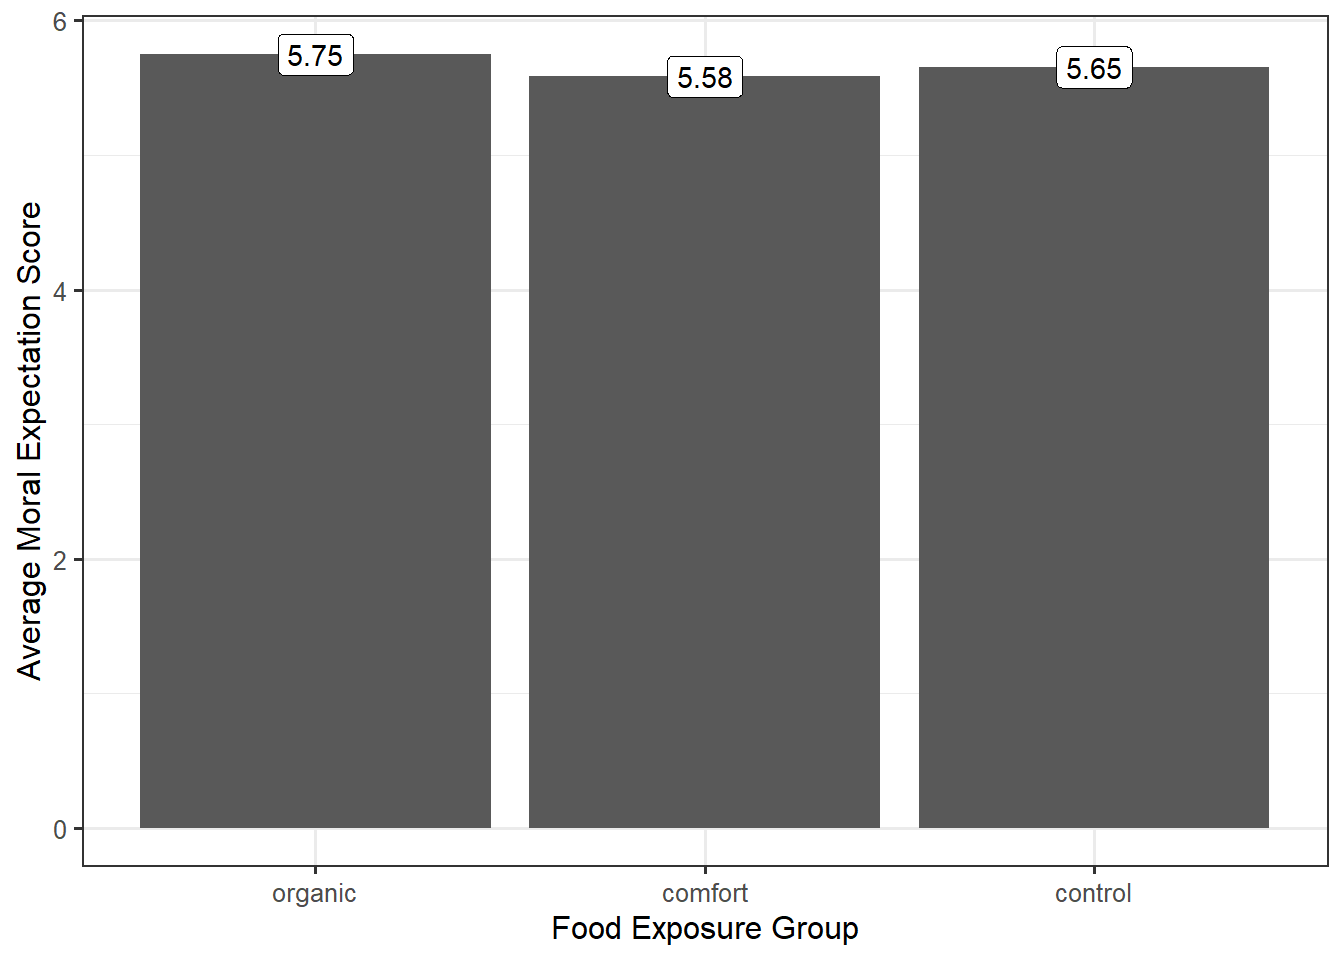
\includegraphics[width=0.8\linewidth]{./Images/anovasummaries-bad-bar-1} 

}

\caption{Illustration of a poor graphic using the Organic Food Case Study; the graphic does not give us a sense of variability.  As a result, it is not clear how different these means really are.}\label{fig:anovasummaries-bad-bar}
\end{figure}

To determine an appropriate graphic, we need to remember that we want to
partition the variability. So, we must not only compare the differences
between the groups but also allow the viewer to get a sense of the
variability within the group. A common way of doing this within the
engineering and sciences is to construct side-by-side boxplots, as
illustrated in Figure \ref{fig:anovasummaries-organic-boxplot}.

\begin{figure}

{\centering 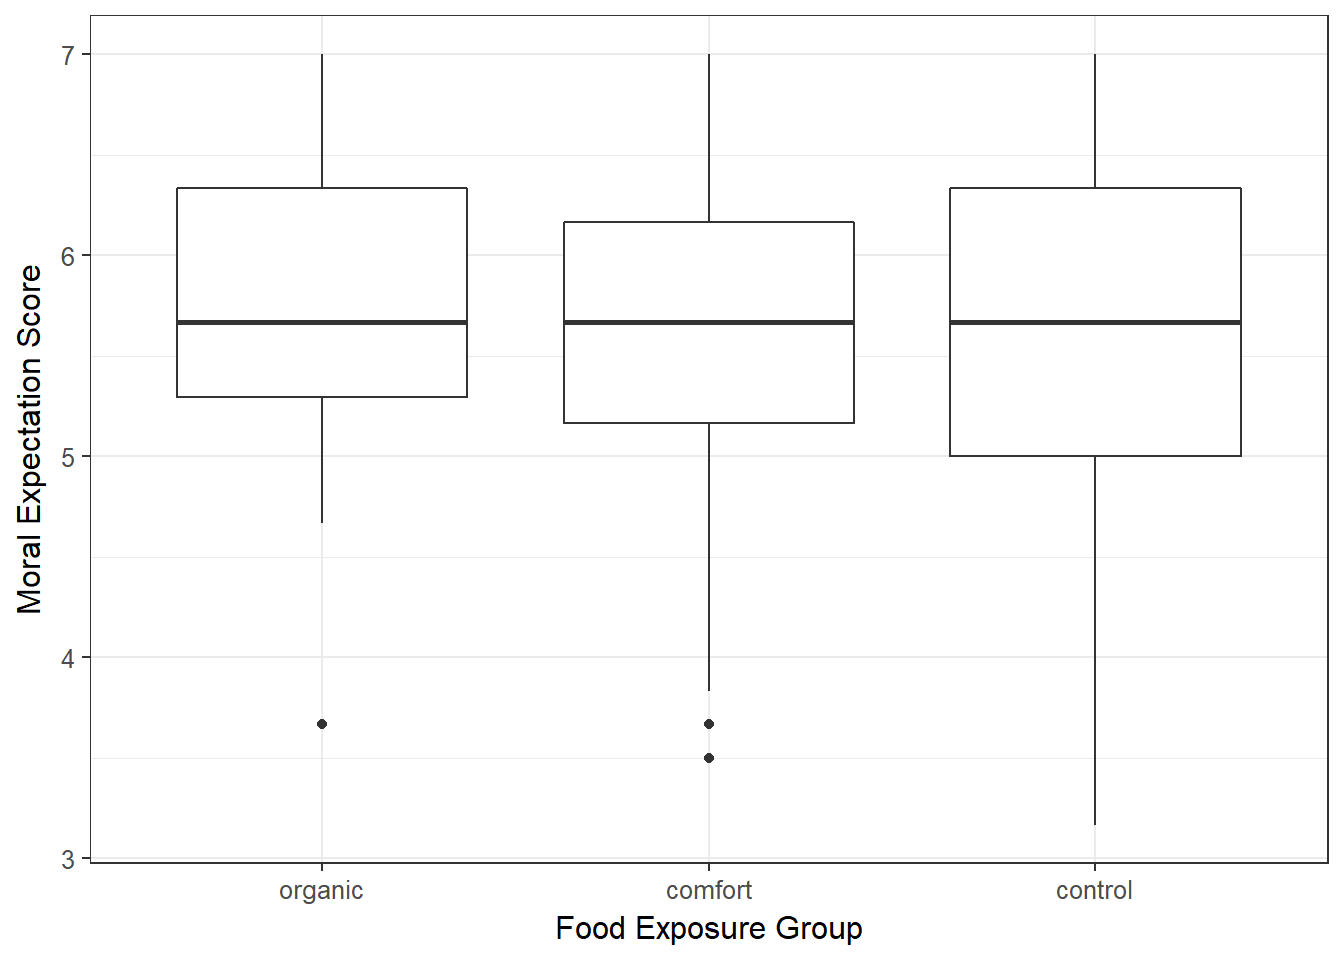
\includegraphics[width=0.8\linewidth]{./Images/anovasummaries-organic-boxplot-1} 

}

\caption{Comparison of the moral expectations for college students exposed to different types of food.}\label{fig:anovasummaries-organic-boxplot}
\end{figure}

From the graphic, we see that the moral expectation scores seem to have
nearly the same pattern in each of the exposure groups. More, the center
of each of the groups is roughly the same. That is, there does not
appear to be any evidence that the type of food to which a subject is
exposed is associated with moral expectations, on average.

Side-by-side boxplots can be helpful in comparing large samples as they
summarize the location and spread of the data. When the sample is
smaller, it can be helpful to overlay the raw data on the graphic in
addition to the summary provided by the boxplot. We might also consider
adding additional information, like the mean within each group. An
alternative to boxplots is to use violin plots which emphasize the shape
of the distribution instead of summarizing it like boxplots. Yet another
option is to construct density plots which are overlayed on one another.
This works when there are only a small number of groups; if the number
of groups is large, then placing the distributions side-by-side is much
more effective. A comparison of these approaches is in Figure
\ref{fig:anovasummaries-organic-comparison}.

\begin{figure}

{\centering 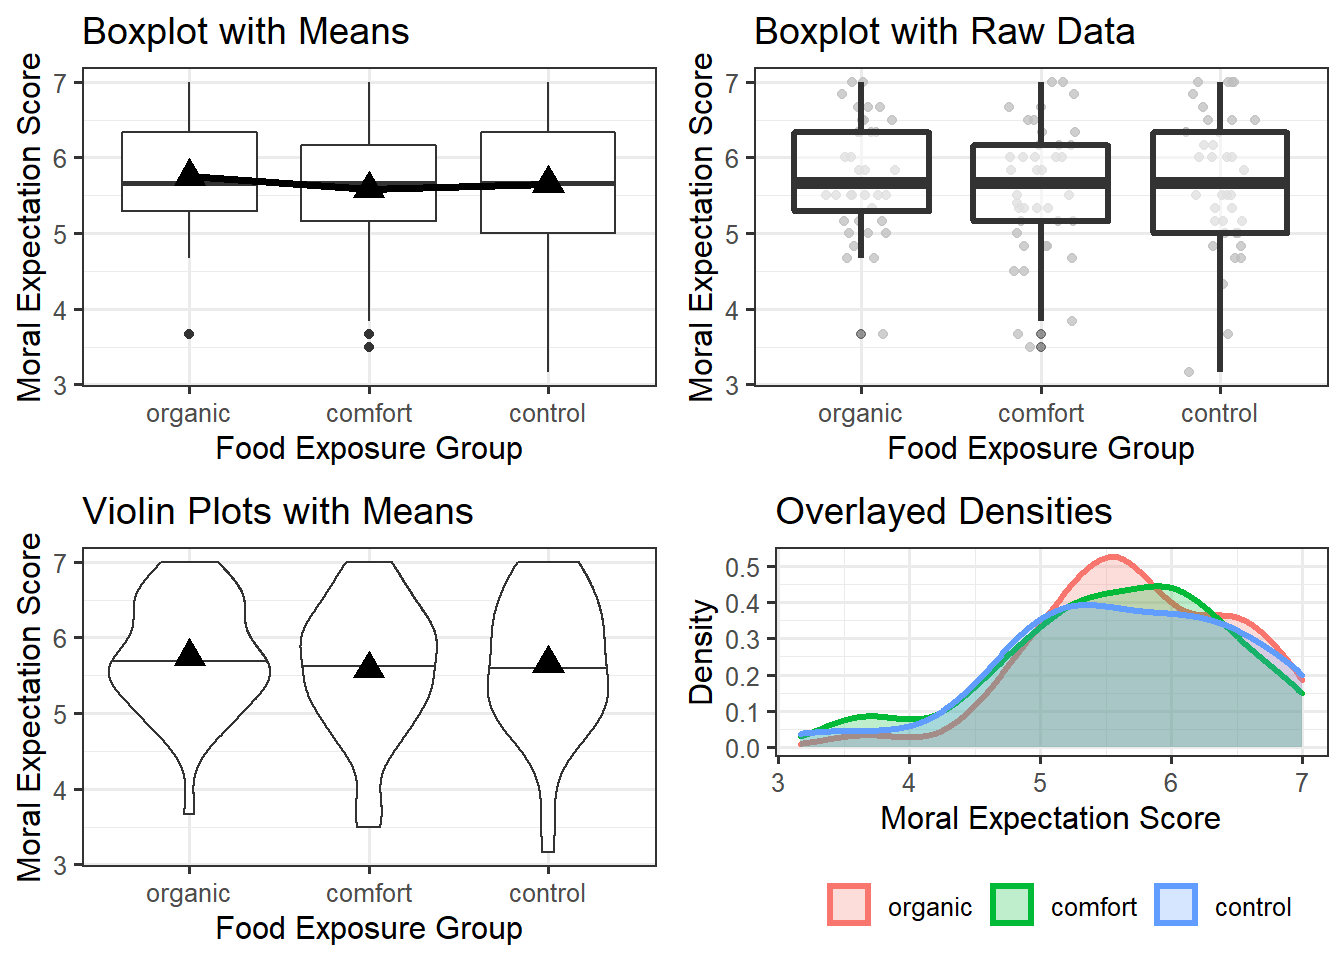
\includegraphics[width=0.8\linewidth]{./Images/anovasummaries-organic-comparison-1} 

}

\caption{Multiple ways to effectively compare the response across multiple groups.}\label{fig:anovasummaries-organic-comparison}
\end{figure}

Each of these plots is reasonable. What makes them useful in addressing
the question is that in each plot, we can compare the degree to which
the groups differ relative to the variability within a group. That is,
we partition the variability. With each plot, we can say that one of the
reasons the groups differ is because of exposure to different food
types; however, this difference is extremely small relative to the fact
that regardless of which food group you were exposed to, the variability
in moral expectations with that group is quite large. Since the
predominant variability in the moral exposure is the variability within
the groups, we would say there is no signal here. That is, there is no
evidence that the average scores differ across food exposure groups.

The key to a good summary is understanding the question of interest and
building a graphic which addresses this question through a useful
characterization of the variability.

\chapter{Quantifying the Evidence}\label{ANOVAteststat}

Figure \ref{fig:anovateststat-boxplots} displays a numeric response
across three groups for two different datasets. Consider the following
question:

\begin{quote}
For which dataset is there \emph{stronger} evidence that the response is
associated with the grouping variable?
\end{quote}

\begin{figure}

{\centering 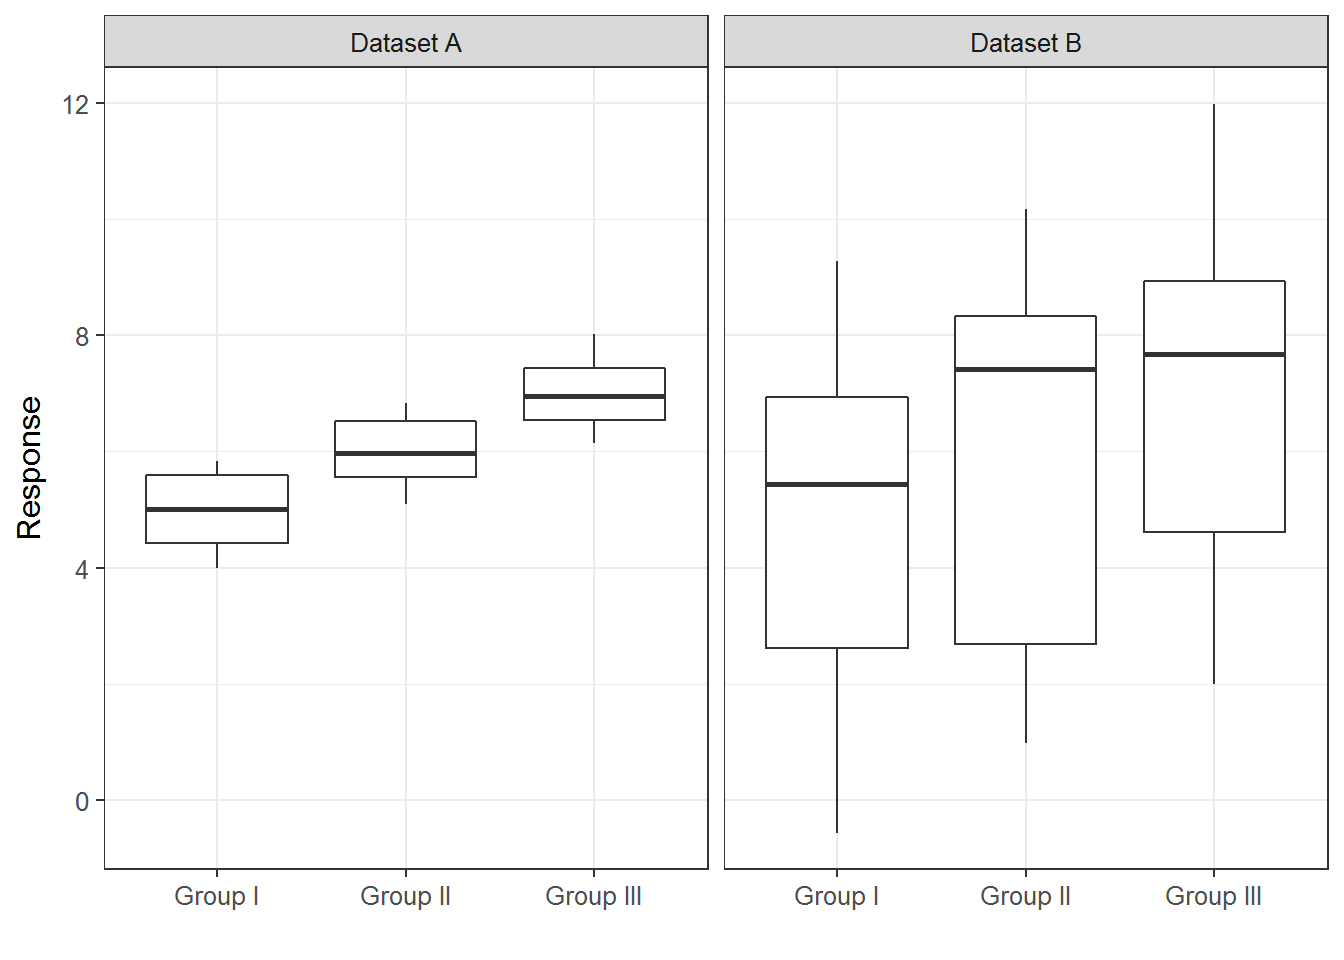
\includegraphics[width=0.8\linewidth]{./Images/anovateststat-boxplots-1} 

}

\caption{Simulated data illustrating that signal strength is determined by partitioning variability. There is a clear signal (difference in the location across groups) for Dataset A but not for Dataset B.}\label{fig:anovateststat-boxplots}
\end{figure}

Nearly everyone will say that Dataset A provides stronger evidence of a
relationship between the grouping variable and the response. We
generated these data such that the mean for Groups I, II and II are 5, 6
and 7, respectively, \emph{for both Datasets A and B}. While there is a
difference, on average, in the response across the groups in both cases,
it is correct that Dataset A provides stronger evidence for that
relationship. The real question is ``what is it that leads everyone to
make the same conclusion when we have not yet discussed how to analyze
this data?'' When we ask students why they feel Dataset A provides
stronger evidence, we typically hear that it is because the ``gaps''
between the groups ``look bigger.'' In essence, that is exactly right!

\section{Partitioning Variability}\label{partitioning-variability}

Subconsciously, when we are deciding whether there is a difference
between the groups, we are partitioning the variability in the response.
We are essentially describing two sources of variability: the
variability in the response caused by subjects belonging to different
groups and the variability in the response within a group (Figure
\ref{fig:anovateststat-partition-variability}). In both Datasets A and B
from Figure \ref{fig:anovateststat-boxplots}, the \textbf{between-group
variability} is the same; the difference in the means from one group to
another is the same in both cases. However, the \textbf{within-group
variability} is much smaller for Dataset A compared to Dataset B.

\begin{figure}

{\centering 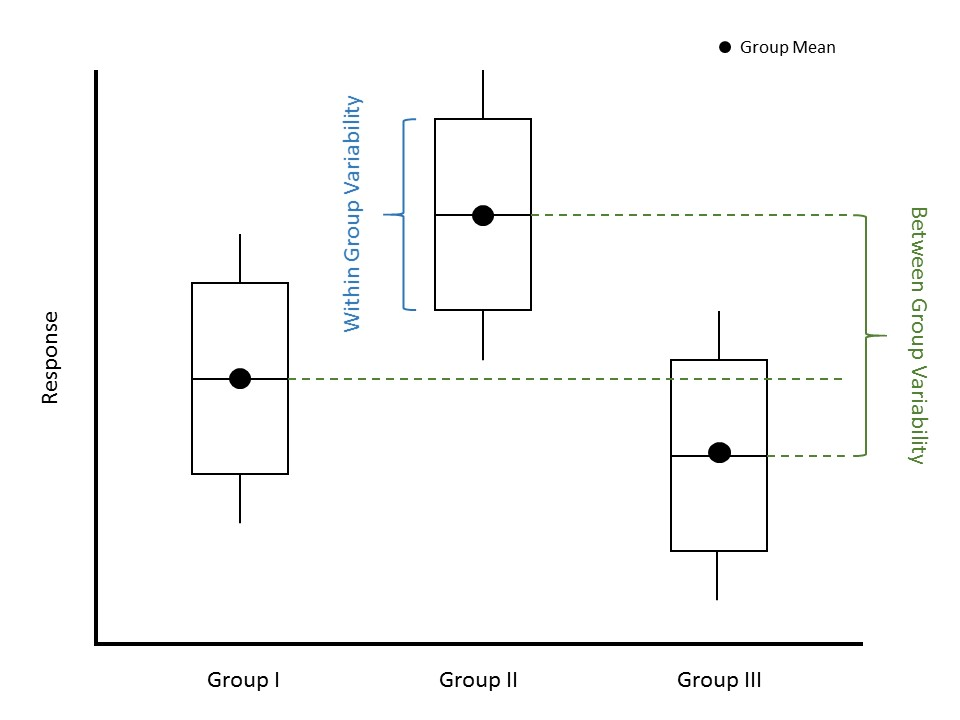
\includegraphics[width=0.8\linewidth]{./images/ANOVATestStat-Partition-Variability} 

}

\caption{Illustration of partitioning the variability in the response to assess the strength of a signal.}\label{fig:anovateststat-partition-variability}
\end{figure}

\BeginKnitrBlock{definition}[Between Group Variability]
\protect\hypertarget{def:defn-between-group-variability}{}{\label{def:defn-between-group-variability}
\iffalse (Between Group Variability) \fi{} }The variability in the
average response from one group to another.
\EndKnitrBlock{definition}

\BeginKnitrBlock{definition}[Within Group Variability]
\protect\hypertarget{def:defn-within-group-variability}{}{\label{def:defn-within-group-variability}
\iffalse (Within Group Variability) \fi{} }The variability in the
response within a particular group.
\EndKnitrBlock{definition}

Figure \ref{fig:anovateststat-boxplots} then illustrates the larger the
variability between groups \emph{relative to} the variability within
groups, the stronger the signal. Quantifying the strength of a signal is
then about quantifying the ratio of these two sources of variability.
Let this sink in because it is completely counter-intuitive. We are
saying that in order to determine if there is a difference in the mean
response across groups, we have to examine variability. Further, a
signal in data is measured by the variability it produces. For this
reason, comparing a quantitative response across a categorical variable
is often referred to as Analysis of Variance (ANOVA).

\BeginKnitrBlock{rmdkeyidea}
Consider the ratio of the variability between groups to the variability
within groups. The larger this ratio, the stronger the evidence of a
signal provided by the data.
\EndKnitrBlock{rmdkeyidea}

\section{Forming a Standardized Test
Statistic}\label{forming-a-standardized-test-statistic}

As we stated above, quantifying the strength of a signal is equivalent
to quantifying the ratio of two sources of variability. Such ratios are
known as \textbf{standardized test statistics}.

\BeginKnitrBlock{definition}[Standardized Test Statistic]
\protect\hypertarget{def:defn-standardized-test-statistic}{}{\label{def:defn-standardized-test-statistic}
\iffalse (Standardized Test Statistic) \fi{} }A ratio of two sources of
variability, or a signal-to-noise ratio. The larger the test statistic,
the stronger the evidence of a signal; said another way, the larger the
test statistic, the stronger the evidence against the null hypothesis.
\EndKnitrBlock{definition}

Based on our observations above, the standardized test statistic for
comparing the mean response across multiple groups has the general form

\begin{equation}
  T = \frac{(\text{Between Group Variability})}{(\text{Within Group Variability})}
  \label{eq:general-test-stat}
\end{equation}

The question we then have before us is the following: how do we measure
these sources of variability? Consider again the hypothesis of interest
for the \protect\hyperlink{CaseOrganic}{Oranic Food Case Study}:

\begin{quote}
\(H_0: \mu_{\text{comfort}} = \mu_{\text{control}} = \mu_{\text{organic}}\)\\
\(H_1:\) At least one \(\mu\) differs from the others
\end{quote}

In order to form the standardized test statistic, let's again think
about what constitutes evidence \emph{against} the null hypothesis. The
more the means differ from one another, the stronger the evidence. But,
in the previous unit, we had a measure for how different values were
from one another --- variance. That is, the \emph{between-group}
variability can be measured by the variance of the means; we call this
the \textbf{Mean Square for Treatment (MSTrt)}.

\BeginKnitrBlock{definition}[Mean Square for Treatment (MSTrt)]
\protect\hypertarget{def:defn-mstrt}{}{\label{def:defn-mstrt} \iffalse (Mean
Square for Treatment (MSTrt)) \fi{} }This captures the between-group
variability in an Analysis of Variance; it is a weighted variance among
the sample means from the various groups. It represents the signal.
\EndKnitrBlock{definition}

Since we do not know the means for each groups (remember, each \(\mu\)
is a parameter), we assess the between group variability within the
sample using the estimates for these parameters --- the sample means.
This is our signal. The larger this variance, the further apart the
means are from one another (agreeing with the alternative hypothesis);
the smaller this variance, the closer the means are (agreeing with the
null hypothesis).

While the numerator provides some measure of the size of the signal, we
need again need to consider how much noise is within the data. Again, in
Figure \ref{fig:anovateststat-boxplots}, the variability between the
means is identical for the two datasets; the signal is stronger for
Dataset A because this variability is larger \emph{with respect to the
noise}. In order to capture the \emph{within-group} variability, we pool
the variances for each group; this is called the \textbf{Mean Square for
Error (MSE)}.

\BeginKnitrBlock{definition}[Mean Square for Error (MSE)]
\protect\hypertarget{def:defn-mse}{}{\label{def:defn-mse} \iffalse (Mean
Square for Error (MSE)) \fi{} }This captures the within-group
variability; it is a pooled estimate of the variance within the groups.
It represents the noise.
\EndKnitrBlock{definition}

Our test statistic in Equation \eqref{eq:general-test-stat} is then
refined to

\begin{equation}
  T = \frac{MSTrt}{MSE}
  \label{eq:anova-test-stat}
\end{equation}

\BeginKnitrBlock{rmdtip}
Consider testing the hypotheses \textgreater{}
\(H_0: \mu_1 = \mu_2 = \dotsb = \mu_k\)\\
\textgreater{} \(H_1:\) At least one \(\mu\) differs from the others

The standardized test statistic of interest is

\[
  T = \frac{MSTrt}{MSE}
\]

where

\[
\begin{aligned}
  MSTrt &= \frac{1}{k-1} \sum_{j=1}^{k} n_j \left(\bar{y}_j - \bar{y}\right)^2 \\
  MSE &= \frac{1}{n-k} \sum_{j=1}^{k} \left(n_j - 1\right) s_j^2
\end{aligned}
\]

and \(n_j\) represents the sample size for the \(j\)-th group,
\(\bar{y}_j\) represents the sample mean for the \(j\)-th group,
\(\bar{y}\) represents the overall mean response across all groups, and
\(s_j^2\) represents the sample variance for the \(j\)-th group.
\EndKnitrBlock{rmdtip}

We note that while mathematical formulas have been provided to add some
clarity to those who think algebraically, our emphasis is \emph{not} on
the computational formulas as much as the idea that we are comparing two
sources of variability.

\section{Obtaining a P-value}\label{obtaining-a-p-value}

Standardized test statistics quantify the strength of a signal, but they
do not allow for easy interpretation. However, with a standardized test
statistic, we are able to compute a p-value to quantify how unlikely our
particular sample is. That is, we need to construct the null
distribution for the standardized test statistic. We need to know what
type of signal we would expect if the null hypothesis were true.
Conceptually, this is no different than it was in Unit I. We consider
running the study again in a world in which all the groups are the same;
for the \protect\hyperlink{CaseOrganic}{Organic Food Case Study}, this
would involve - Obtaining a new sample of students. - Randomizing each
student to one of the three groups at random, all showing the same
foods. - Having each student answer a questionnaire regarding moral
dilemmas. - Summarize the data by computing a standardized test
statistic.

Notice the difference in step 2 above compared to what actually happened
in the real study. In the real study, each group had a different set of
foods. This was to answer the question about whether there is a
difference in the groups. However, in order to construct the \emph{null
distribution}, we need to force all groups to be the same. This could be
accomplished by showing every group the same set of foods. The primary
difference in this unit is that the strength of the signal is measured
through a standardized test statistic. After repeating the above steps
over and over again, we determine how often the recorded standardized
test statistics exceeded the value we obtained in our actual sample.

Figure \ref{fig:anovateststat-pvalue} represents the null distribution
of the standardized test statistic. Again, these are values of the
standardized test statistic we would expect if there were no
relationship between the food categories to which the students were
exposed and their moral score. We are then interested in finding out if
the observed dataset is consistent with these expectations.

\begin{figure}

{\centering 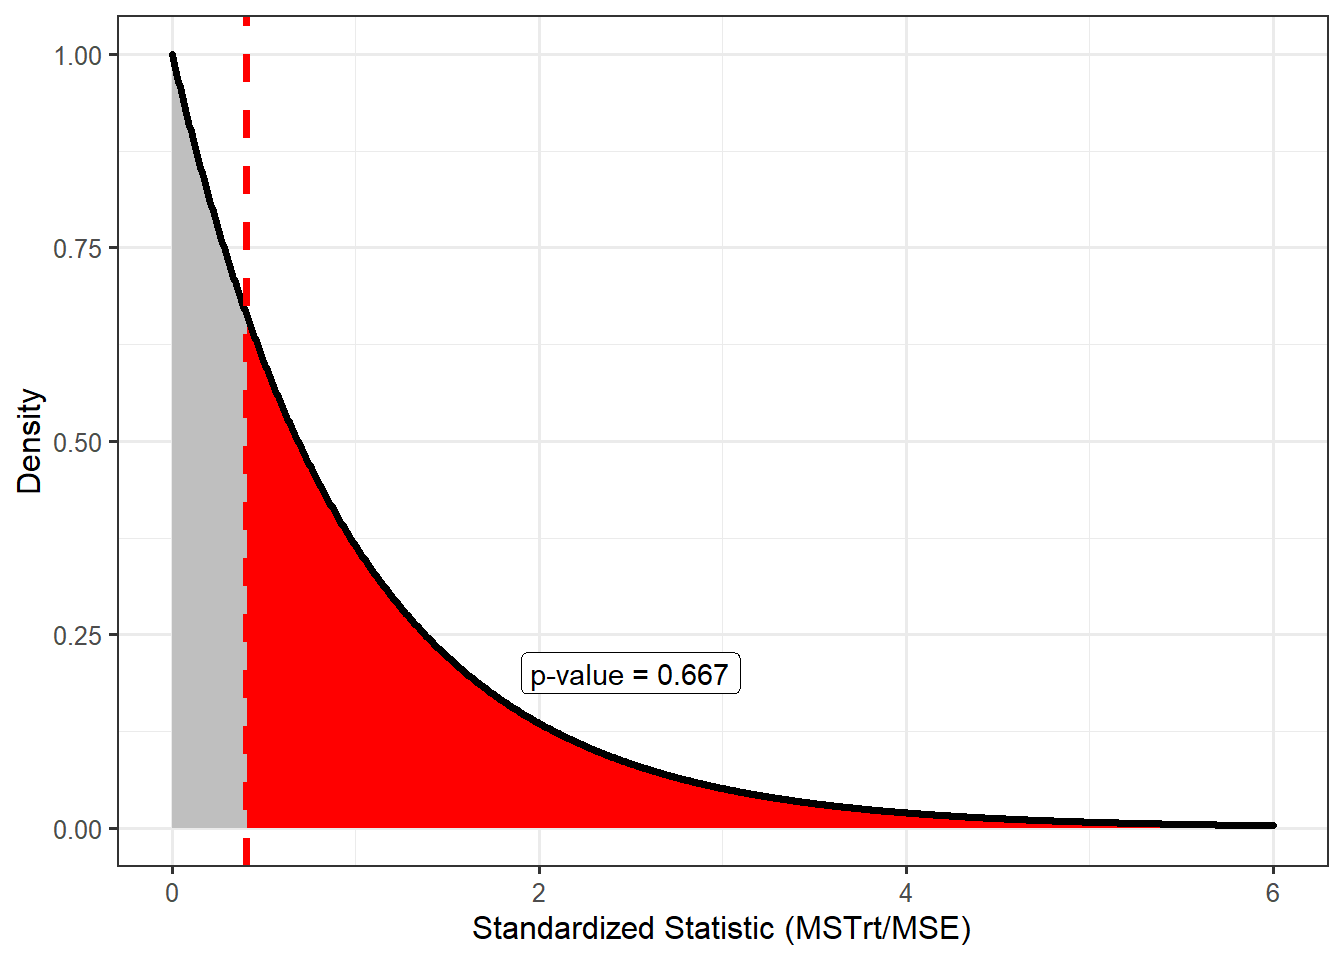
\includegraphics[width=0.8\linewidth]{./Images/anovateststat-pvalue-1} 

}

\caption{Computation of the p-value for the Organic Food Case Study by simulating the null distribution.  The null distribution is based on 5000 replications.}\label{fig:anovateststat-pvalue}
\end{figure}

Notice that in our data, we observed a standardized test statistic of
0.41; based on the null distribution, we would expect a signal this
strong or stronger about 66.9\% of the time \emph{when no signal existed
at the population} (by chance alone). That is, our data is quite
consistent with what we would expect under the null hypothesis. There is
no evidence of a relationship between the type of food a student is
exposed to and their moral expectations, on average.

Again, conceptually, this is similar to what we saw in the previous
unit. We are simply determining how likely our data is under the null
hypothesis. However, unlike the previous unit, it may not be clear how
we actually model this null distribution. If we cannot physically redo
the study, how can we construct this model? In order to understand this,
we must consider a different model --- that for the data generating
process. This is the topic of the next chapter.

\chapter{Building the Statistical Model}\label{ANOVAmodel}

The numerical summaries of any study are subject to sampling
variability. That is, if we were to repeat the study with new subjects,
the statistics we compute would almost certainly change to some degree.
The key to feeling confident in our results is to quantify the
variability in our estimates; this was the argument made in Chapters
\ref{SamplingDistns} and \ref{NullDistns}. The goal of any statistical
analysis is then to develop a model for the sampling (or null)
distribution of a statistic. Often times, this requires modeling the
data-generating process as a precursor. As in any other discipline,
statistical models simplify the process being modeled by making certain
assumptions. In this chapter, we develop a model that will help us make
inference about the mean of several populations.

\section{General Formulation}\label{general-formulation}

Consider dropping a tennis ball from the top of a 50-meter building and
recording the time required before the ball hits the ground. Applying
the principles learned in a first course in physics, we would be able to
compute the time precisely using the formula
\[\text{time} = \sqrt{\frac{2(\text{distance})}{9.8}}\]

where \(9.8 m/s^2\) is the acceleration due to gravity; further, this
formula works regardless of the mass of the object. Plugging 50 meters
into the equation yields a time of 10.2 seconds. If we were to drop a
second tennis ball from the same building, the formula tells us that it
will also take 10.2 seconds to hit the ground below. This is known as a
\textbf{deterministic} system since entering a constant input always
results in the same output.

\BeginKnitrBlock{definition}[Deterministic Process]
\protect\hypertarget{def:defn-deterministic-process}{}{\label{def:defn-deterministic-process}
\iffalse (Deterministic Process) \fi{} }One which is completely
determined by the inputs. That is, entering the same input twice will
always result in the same output with certainty.
\EndKnitrBlock{definition}

This is a model; it simplifies extremely complex processes involving the
gravitational pull between objects and works reasonably well. However,
it does not always match reality. If we were to repeatedly drop tennis
balls from the same 50-meter building and record the time before hitting
the ground, we might find that the time differs slightly from one ball
to the next. There are several reasons why our observed responses do not
line up directly with those predicted by the above equation; for
example, our device for measuring time may be subject to some
measurement error, a strong gust of wind could alter the results (while
the above equation assumes no air resistance), or the person dropping
the ball may have inadvertantly increased the initial velocity of the
ball. These reasons, and others, contribute to the observations not
lining up with the model. That is, there is associated noise in the
resulting measurements. A model which incorporates this noise might be
written as
\[\text{time} = \sqrt{\frac{2(\text{distance})}{9.8}} + \text{noise}\]

where the noise is not a known quantity. As a result, this is a
\textbf{stochastic} model as the same value for distance may result in
different outputs each time.

\BeginKnitrBlock{definition}[Stochastic Process]
\protect\hypertarget{def:defn-stochastic-process}{}{\label{def:defn-stochastic-process}
\iffalse (Stochastic Process) \fi{} }One which has an element of
randomness. That is, the resulting output of the system cannot be
predicted with certainty.
\EndKnitrBlock{definition}

This leads us to our general formulation for a statistical model:

\begin{equation}
  \text{Response} = f(\text{variables, parameters}) + \text{noise}
  \label{eq:general-model}
\end{equation}

The response we observe is the result of two components:

\begin{itemize}
\tightlist
\item
  A deterministic component which takes the form of a function of
  variables and unknown parameters. It is often this component on which
  we would like to make inference.
\item
  A stochastic component which captures the unexplained variability in
  the data generating process.
\end{itemize}

Since the noise is a random element, it has a distribution. We often
make additional assumptions on the structure of this distribution to
enable inference on the deterministic component of the model. We discuss
this later in the chapter.

This general model adheres to the idea of partitioning the variability
in the response. It says that a part of the reason the responses differ
between subjects is because they have different variables (remember,
parameters are fixed for all subjects in a population); part of the
reason is unexplained noise. The overall goal of a statistical model is
to give an explanation for why the data is what it is. How did it come
to be? What process generated the values I have observed? Our
statistical model says that these values have some deterministic
component plus some additional noise we cannot explain. We now turn
towards employing this model in the case of comparing the mean response
for multiple groups.

\section{Statistical Model for A Quantitative Response and a Categorical
Predictor}\label{statistical-model-for-a-quantitative-response-and-a-categorical-predictor}

For the \protect\hyperlink{CaseOrganic}{Organic Food Case Study}, we are
comparing the moral expectations (quantitative response) for different
food exposures (levels of a categorical variable). Our model for the
data-generating process is best understood in light of the graphic we
used to display the data (see Figure \ref{fig:anovamodel-organic-plot}).

\begin{figure}

{\centering 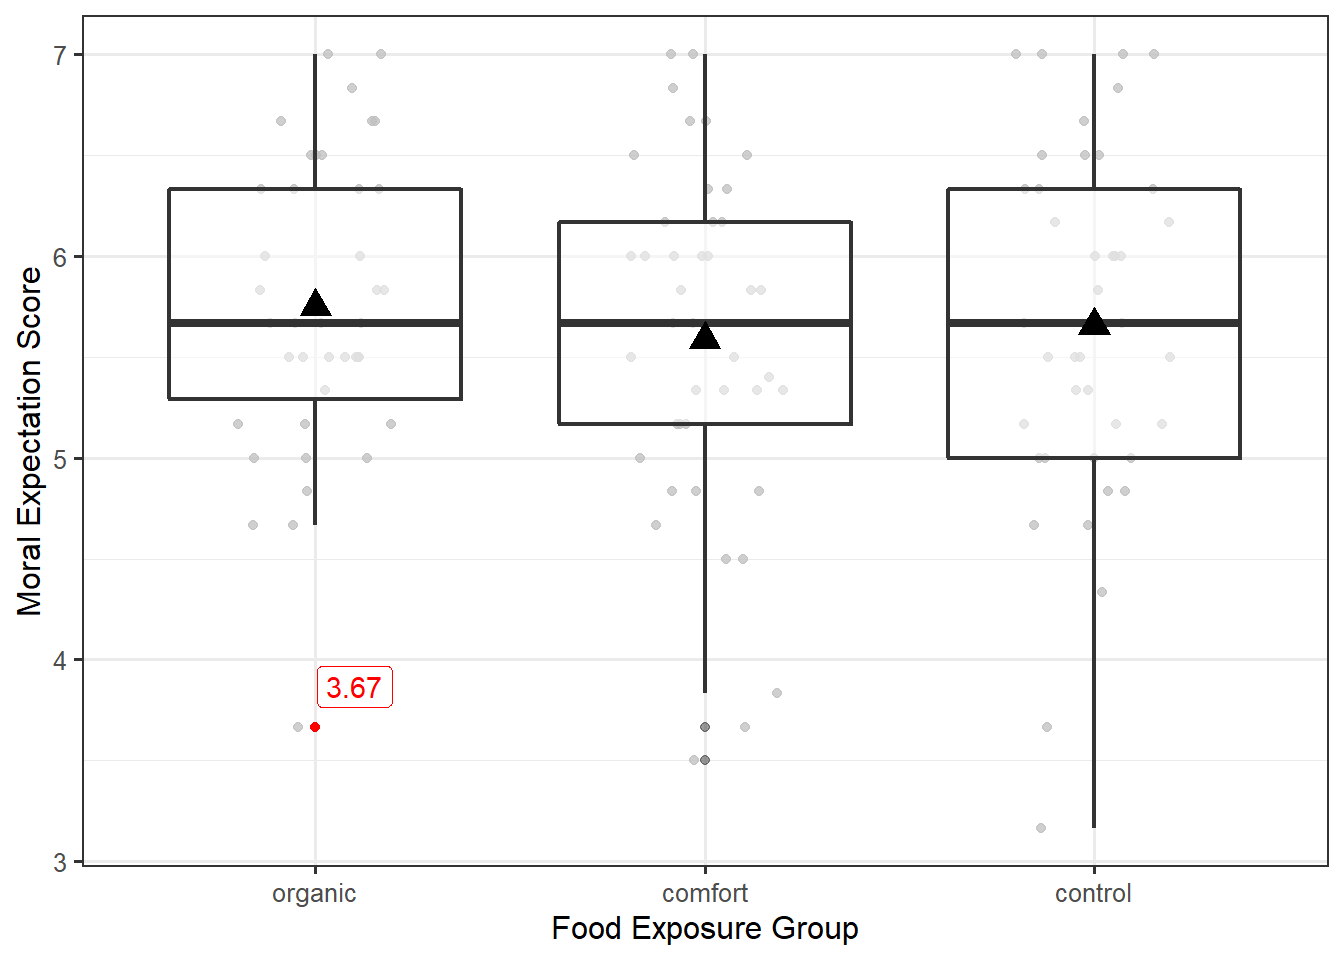
\includegraphics[width=0.8\linewidth]{./Images/anovamodel-organic-plot-1} 

}

\caption{Moral expectation scores for students following exposure to various food types.}\label{fig:anovamodel-organic-plot}
\end{figure}

Let's consider how the value 3.67, highlighted red in Figure
\ref{fig:anovamodel-organic-plot}, was generated. As discussed
previously, there are two sources of variability in the moral
expectation scores (two reasons that the values are not all the same).
One source is the fact that different subjects had different exposures.
That is, one reason the value 3.67 differs from others observed is
because this subject belongs to the organic group and not the comfort or
control exposure groups. As this is something we can explain, it goes
into the deterministic portion of the model; it is a function of known
variables (group exposure). Let the function \(f(\cdot)\) be such that
the input is the group exposure for the \(i\)-th subject and the output
is the mean moral expectation score for that group; this can be
represented as a piecewise function: \[
f\left((\text{Food Exposure Group})_i\right) = \begin{cases}
  \mu_1 & \text{if i-th subject exposed to organic foods} \\
  \mu_2 & \text{if i-th subject exposed to control foods} \\
  \mu_3 & \text{if i-th subject exposed to comfort foods} \end{cases}
\]

Notice that \(f(\cdot)\) involves both a variable of interest as well as
parameters of interest --- the mean response \(\mu_1, \mu_2, \mu_3\) for
each of the three groups. This function is perfectly acceptable, but it
is cumbersome to write in a shortened form. Notice how the function
works: it receives an input regarding which group, and it directs you to
the appropriate parameter as an output. We can write this in a compact
way as \[
f\left((\text{Food Exposure Group})_i\right) = \sum_{j=1}^{3} \mu_j \mathbb{I}\left(\text{i-th subject in food exposure group j}\right)
\]

where \(\mathbb{I}(\cdot)\) is the indicator function taking value 1 if
the event occurs and 0 otherwise.

\BeginKnitrBlock{rmdkeyidea}
The deterministic component of a statistical model incorporates the
parameters which govern the question of interest. It is built to explain
differences in the response based on differences in group membership or
other characteristics of the subjects.
\EndKnitrBlock{rmdkeyidea}

This is the deterministic part of the model, as inputing the same group
always results in the same output --- the unknown parameter
characterizing the mean response for the group. This, however, only
captures one reason we feel the responses differ across subject. This
deterministic component says that every single person exposed to the
same food group should have the same moral expectations. It does not
explain why subjects within the organic group do not all share the
average moral expectation score. This source of variability is something
we cannot fully explain but attribute to natural variability in this
group or measurement error in how we obtained the response. In order to
capture this, we add noise to the system, and we allow this noise to be
a random variable which is unique to each subject within the population.
Letting \(\epsilon_i\) represent the noise accompanying the response of
the \(i\)-th subject, we can now extend the model in Equation
\eqref{eq:general-model} to accommodate these two sourses of variability
and obtain \[
\text{(Moral Expectation Score)}_i = \sum_{j=1}^3 \mu_j \mathbb{I}(\text{i-th subject in food exposure group j}) + \epsilon_i
\]

This may be written in shorthand (suppressing the parameters and noise)
as \[ \text{Moral Expectation Score} \sim \text{Food Exposure Group}\]

\BeginKnitrBlock{rmdkeyidea}
The stochastic component of a statistical model captures the unexplained
variability due to natural variability in the population or measurement
error in the response.
\EndKnitrBlock{rmdkeyidea}

\BeginKnitrBlock{rmdtip}
In general, given a quantitative response variable \(y\), our model for
the data generating process comparing this variable across several
levels of a factor is
\[y_i = \sum_{j=1}^k \mu_j \mathbb{I}(\text{i-th subject in factor level j}) + \epsilon_i\]
\EndKnitrBlock{rmdtip}

In general, students struggle with the fact that we have two different
models floating around. Currently, we are modeling the data-generating
process. This model is used to develop a secondary model of the sampling
distribution (or null distribution) of a statistic of interest. It is
this secondary model that is actually necessary in order to conduct
inference; the model for the data-generating process is simply a
stepping stone to the model of interest.

\section{Conditions on the Error
Distribution}\label{conditions-on-the-error-distribution}

In our model for the data-generating process we incorporated a component
\(\epsilon\) to capture the noise within each group. Since the error is
a random variable (stochastic element), we know it has a distribution.
We typically assume a certain structure to this distribution. The more
assumptions we are willing to make, the easier the analysis, but the
less likely our model is to be applicable to the actual data-generating
process we have observed. The conditions we make dictate how we conduct
inference (the computation of a p-value or confidence interval).

The first condition we consider is that the noise attributed to one
observed individual is \textbf{independent} of the noise attributed to
any other individual observed. That is, the amount of error in any one
individual's response is unrelated to the error in any other response
observed. It is easiest to understand this condition by examining a case
when the condition would not hold.

\BeginKnitrBlock{definition}[Independence]
\protect\hypertarget{def:defn-independence}{}{\label{def:defn-independence}
\iffalse (Independence) \fi{} }Two variables are said to be independent
when the likelihood that one variable takes on a particular value does
not depend on the value of the other variable.
\EndKnitrBlock{definition}

\BeginKnitrBlock{example}[Programming Speed]
\protect\hypertarget{exm:ex-programming}{}{\label{exm:ex-programming}
\iffalse (Programming Speed) \fi{} }Suppose we are conducting a study to
compare the speed required to complete a particular programming task in
two different languages: Python and R. We obtain a sample of 100
programmers previously exposed to Java but neither Python nor R. We ask
each programmer to complete a programming exercise in Python and record
the time required to successfully complete the task. Then, we ask each
programmer to perform the same task in R and record the time required to
successfully complete the task.

The model for the data generating process would be \[
(\text{Time})_i = \mu_1 \mathbb{I}(\text{i-th task programmed in Python}) + \mu_2 \mathbb{I}(\text{i-th task programmed in R}) + \epsilon_i
\]

Given the method in which the data was collected, it would not be
reasonable to assume the errors are independent of one another. Some
programmers are naturally faster than others. A programmer with a below
average (negative \(\epsilon\)) time in Python will most likely have a
below average (negative \(\epsilon\)) time in R on the same task.
Therefore, there is a relationship between the errors for some of the
observations taken. This violates the independence condition.
\EndKnitrBlock{example}

The second condition that is typically placed on the distribution of the
errors is that the variability of the responses is similar within each
group. This assumption is known as \textbf{homoskedasticity}.

\BeginKnitrBlock{definition}[Homoskedasticity]
\protect\hypertarget{def:defn-homoskedasticity}{}{\label{def:defn-homoskedasticity}
\iffalse (Homoskedasticity) \fi{} }Also known as ``constant variance,''
this assumption states that the variability of error terms for
individuals within a group is the same across all groups.
\EndKnitrBlock{definition}

Practically, this means that the responses in one group are not
dramatically more variable than any other group (the width of the box
portion of a boxplot should be roughly the same across groups). This
condition ensures that the precision of the measurements is roughly
similar. In fact, we made use of this assumption in the construction of
our standardized test statistic \[T = \frac{MSTrt}{MSE}\]

since MSE was a pooled estimate of the variability. If we were not
willing to assume that the variabilities were similar, we would not
construct a pooled estimate. This also highlights that the MSE is an
estimate of the variability of observations within any group when this
condition is satisfied.

\section{Simulating the Null
Distribution}\label{simulating-the-null-distribution}

We note that this section is a bit more technical than other sections.
We want to give the reader a feel for the computational aspect of
simulating the null distribution. However, understanding conceptually
that we are repeating the study in a world in which the null hypothesis
is true is sufficient for interpreting a p-value.

Under the above conditions, we can model the null distribution of our
standardized test statistic. The key here is to lean on our data
generating process. Consider the \protect\hyperlink{CaseOrganic}{Organic
Food Case Study}. \emph{If the null hypothesis is true}, then we have
that
\[\mu_{\text{organic}} = \mu_{\text{comfort}} = \mu_{\text{control}}\]

Let's define this common mean to be \(\mu\); we do not know what this
value is, but it is common to all groups. Therefore, \emph{if the null
hypothesis is true}, we have that the data generating process reduces to

\begin{equation}
  \text{(Moral Expectation Score)}_i = \mu + \epsilon_i
  \label{eq:null-model}
\end{equation}

Therefore, we can generate data according to this model. We can replace
\(\mu\) by our best estimate --- the sample mean response across all
observations regardless of their group. It simply remains to determine
how to approximate a random variable from the noise distribution. In
order to do this, we need estimates of the errors, known as
\textbf{residuals}.

\BeginKnitrBlock{definition}[Residual]
\protect\hypertarget{def:defn-residual}{}{\label{def:defn-residual}
\iffalse (Residual) \fi{} }The difference between the observed response
and the predicted response (estimated deterministic portion of the
model). Residuals approximate the noise in the data-generating process.
\EndKnitrBlock{definition}

The deterministic component of the model gives a way of predicting the
response. For example, consider the
\protect\hyperlink{CaseOrganic}{Organic Food Case Study}; the data is
reproduced in Figure \ref{fig:anovamodel-organic-boxplot}. Based on the
data available, if a subject were to be exposed to organic foods, we
would expect their moral expectation score to be 5.66; this is the
average observed among individuals randomized to this treatment within
our study.

\begin{figure}

{\centering 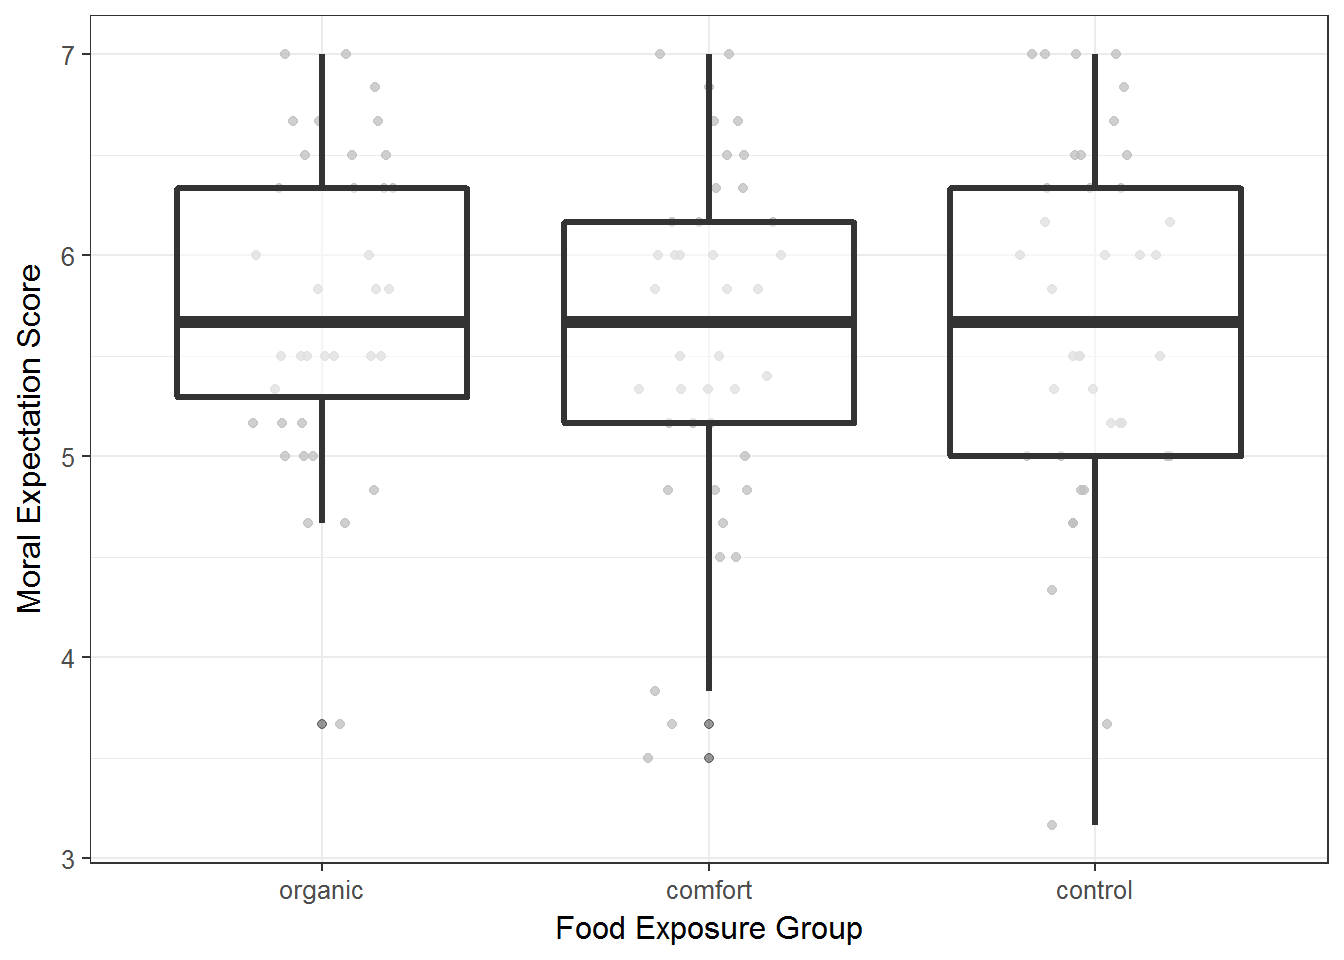
\includegraphics[width=0.8\linewidth]{./Images/anovamodel-organic-boxplot-1} 

}

\caption{Comparison of the moral expectations for college students exposed to different types of food.}\label{fig:anovamodel-organic-boxplot}
\end{figure}

That is, we can define the \textbf{predicted value} for \(i\)-th
observation in our study as \[
\widehat{y}_i = \sum_{j=1}^{3} \bar{y}_j \mathbb{I}(\text{i-th subject in food exposure group j})
\]

and the corresponding residual as \[
e_i = y_i - \widehat{y}_i
\]

Let's not get lost in the mathematical notation; the residual here is
simply the difference between the response of the subject and the
average response for their corresponding group.

The key idea here is that residuals approximate the unseen error.
Therefore, if we take this error and perturb it (the details of which
are beyond the scope of this course), we can generate new data. A new
dataset, generate under the null hypothesis, can then be constructed as
\[
y_i^* = \bar{y} + e_i^*
\]

where \(y_i^*\) is then a new observation constructed by taking a mean
and adding a perturbed version of the residual for that observation.
Notice that each newly generated response has the same mean (so that the
null is true). We then take this new dataset and compute the
standardized test statistic as before and record it. Then, we repeat
this process over and over again until we have constructed the null
distribution. This gives us a sense of the p-value.

\section{Recap}\label{recap}

We have covered a lot of ground in this chapter, and it is worth taking
a moment to summarize the big ideas. In order to construct a model for
the null distribution of the standardized test statistic, we took a step
back and modeled the data generating process. Such a model consists of
two components: a deterministic component explaining the differences
between groups and a stochastic component capturing the noise in the
system.

Certain conditions are placed on the distribution of the noise in our
model. Using these assumptions, we can generate data which adheres to
the null hypothesis. Therefore, we can obtain an empirical model that
suggests what values of a test statistic we might expect.

\chapter{Classical ANOVA Model}\label{ANOVAclassical}

In the previous chapter, we developed a model for a quantitative
response as a function of a categorical predictor. Specifically, suppose
we are comparing a quantitative response across \(k\) levels of a factor
of interest. Our model has the form
\[(\text{Response})_i = \sum_{j=1}^{k} \mu_j \mathbb{I}\left(\text{i-th subject belongs to group j}\right) + \epsilon_i\]

where \(\epsilon\) is a random variable capturing the noise in the
data-generating process. In order to perform inference, we made two
assumptions on this error term:

\begin{itemize}
\tightlist
\item
  The error in one observation is independent of the error in any other
  observation.
\item
  The variability in the error is constant across groups.
\end{itemize}

This allowed us to empirically model the null distribution of our
standardized test statistic \[T = \frac{MSTrt}{MSE}\] through
simulation. This approach is completely valid; however, it has been
shown that such empirical models can be unstable in small sample sizes.
When we do not have the resources to obtain a large sample, we can
improve our model of the sampling distribution (or null distribution) of
a statistic through additional modeling assumptions. In this unit, we
discuss an additional modeling assumption that is common in the
engineering and scientific disciplines.

\section{Modeling the Population}\label{modeling-the-population}

Before we delve into the details, let's set the stage for the bigger
story being told. Recall that our goal is to say something about the
population using a sample. We have developed a process to address this
goal:

\begin{enumerate}
\def\labelenumi{\arabic{enumi}.}
\tightlist
\item
  Frame our question through a parameter of interest.
\item
  Collect data that allows us to estimate the parameter using the
  analogous statistic within the sample.
\item
  Summarize the variability in the data graphically.
\item
  Quantify the variability in the statistic through modeling the
  sampling distribution (or null distribution).
\item
  Using the sampling distribution (or null distribution), quantify the
  evidence in the sample.
\end{enumerate}

This process is wrapped up in our \emph{Five Fundamental Ideas of
Inference} and the \emph{Distributional Quartet}. The key step in this
process is quantifying the variability by modeling the \emph{sampling
distribution} (or \emph{null distribution}). We have described the
construction of these models empirically, through repeating the study by
appropriately resampling the data available.

Our goal is still to model the sampling distribution (or null
distribution); that is the key inferential step. Instead of building an
empirical model, we can construct an analytical (exact) model through an
additional step: modeling the population directly.

\BeginKnitrBlock{rmdkeyidea}
A model for the sampling distribution of a statistic can often be
obtained by placing a model on the distribution of the population.
\EndKnitrBlock{rmdkeyidea}

So, we have two models; the model for the distribution of the population
is simply a stepping stone to what we really need, a model for the
sampling distribution of the statistic. It is important to separate
these steps. We are not interested in directly modeling the population;
we do it in order to construct a model for the sampling distribution.

There is one other distinction to make: a model for the population is
\emph{always} an assumption. We hope that the data is consistent with
this assumption in order to apply the resulting model for the sampling
distribution.

\section{Adding the Assumption of
Normality}\label{adding-the-assumption-of-normality}

The sub-field of mathematics known as probability is the discipline of
modeling randomness. In particular, we make use of probability to model
a distribution. In order to get a feel for probability models, consider
the following example.

\BeginKnitrBlock{example}[Iris Characteristics]
\protect\hypertarget{exm:ex-iris}{}{\label{exm:ex-iris} \iffalse (Iris
Characteristics) \fi{} }The discipline of statistics began in the early
1900's primarily within the context of agricultural research. Edgar
Anderson was a researcher investigating the characteristics of the iris.
He had collected measurements on over one hundred iris flowers,
including their petal length and width and their sepal length and width.
The sepal is the area (typically green) beneath the petal of a flower.
It offers protection while the flower is budding and then support for
the petals after the flower blooms.
\EndKnitrBlock{example}

Figure \ref{fig:anovaclassical-iris-histogram} is a histogram of the
sepal width for the iris plants observed by Edgar Anderson; overlayed is
the density estimate for the same dataset which we have described as a
smoothed histogram. This smoothed histogram is estimated from the data;
it is an empirical model of the distribution.

\begin{figure}

{\centering 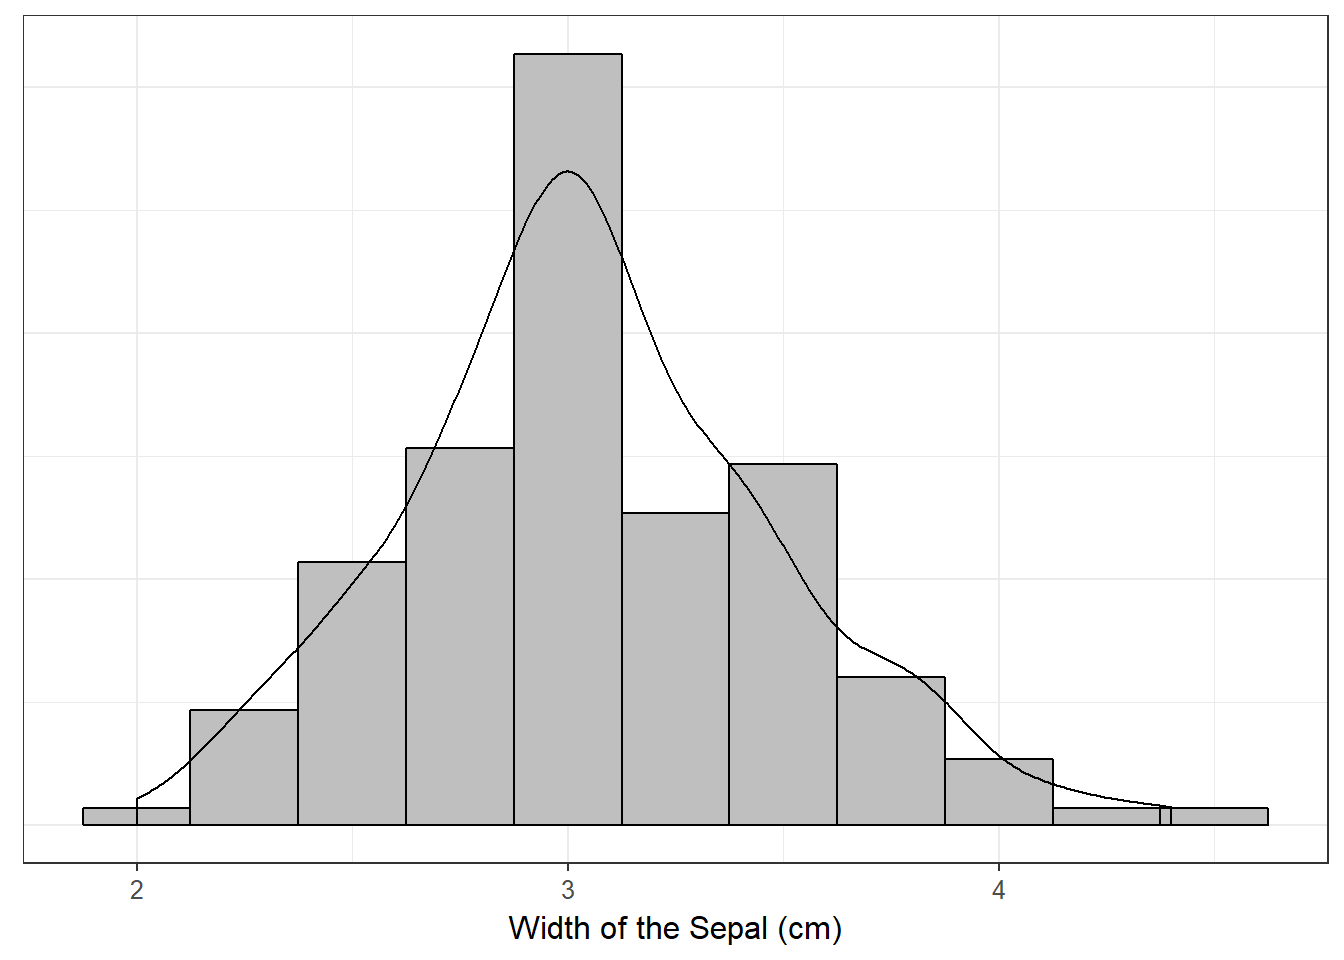
\includegraphics[width=0.8\linewidth]{./Images/anovaclassical-iris-histogram-1} 

}

\caption{Summary of the distribution of sepal widths for a sample of irises.}\label{fig:anovaclassical-iris-histogram}
\end{figure}

Probability models are analytical models for the distribution of a
variable. Instead of constructing a density using data, we probability
theory posits a functional form for the density (subject to certain
constraints that are beyond the scope of this course). For example,
Figure \ref{fig:anovaclassical-iris-normal} overlays the following
function on top of the the iris data:

\[f(x) = \frac{1}{\sqrt{0.380\pi}} e^{-\frac{1}{0.380}(x - 3.057)^2}\]

\begin{figure}

{\centering 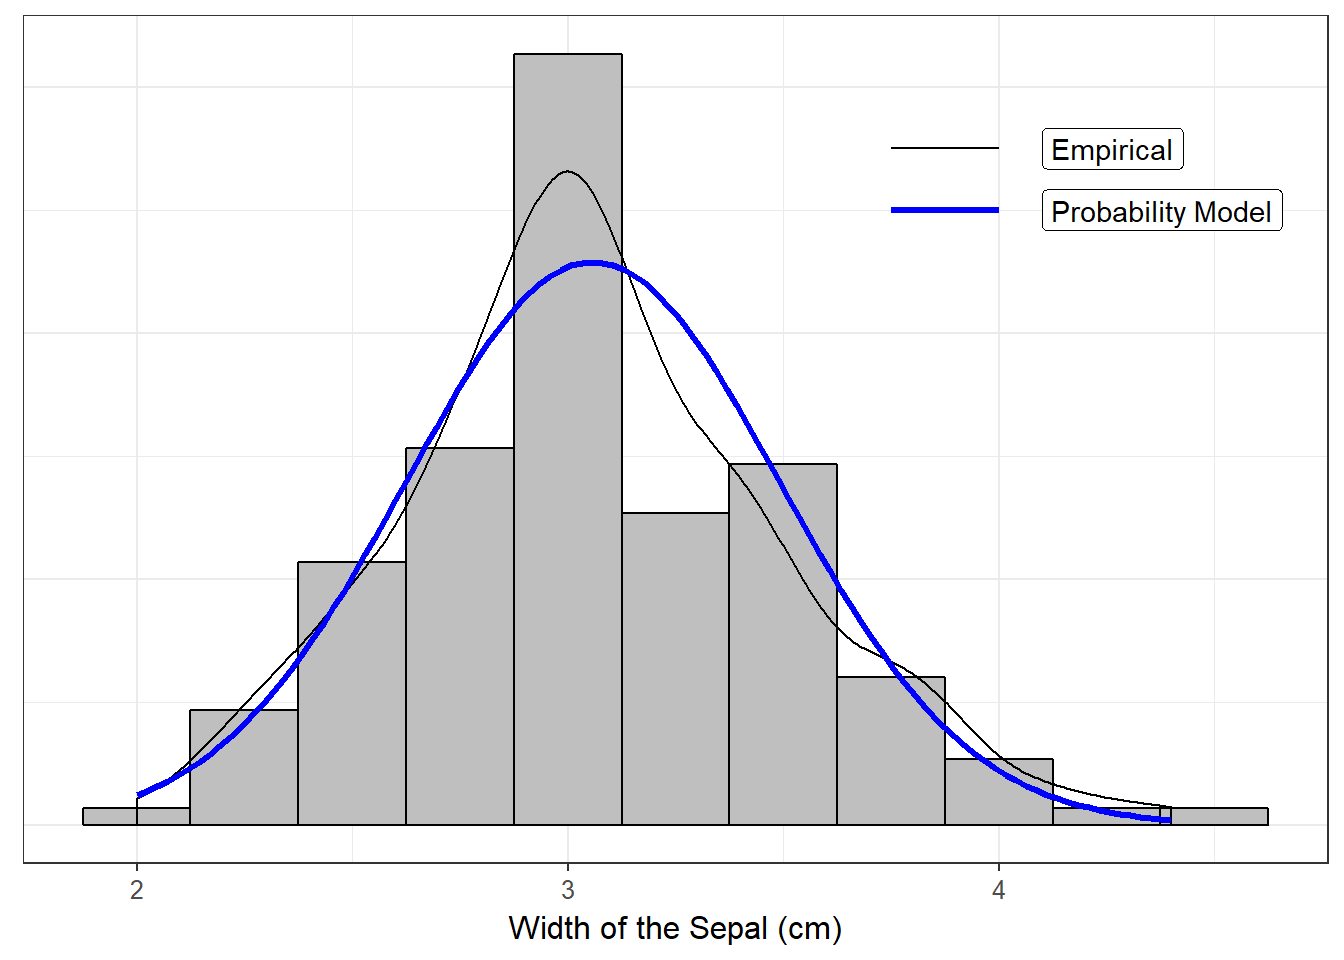
\includegraphics[width=0.8\linewidth]{./Images/anovaclassical-iris-normal-1} 

}

\caption{Summary of distribution  the sepal widths for a sample of irises with a probability model overlayed.}\label{fig:anovaclassical-iris-normal}
\end{figure}

While this model for the density is not perfect, we note that it does
capture many of the characteristics present in the data. This particular
model, characterized by the bell-shape density, is known as the
\textbf{Normal Distribution}.

\BeginKnitrBlock{definition}[Normal Distribution]
\protect\hypertarget{def:defn-normal-distribution}{}{\label{def:defn-normal-distribution}
\iffalse (Normal Distribution) \fi{} }Also called the Gaussian
Distribution, this probability model is popular for modeling noise
within a data-generating process. It has the following characteristics:

\begin{itemize}
\tightlist
\item
  It is bell-shaped.
\item
  It is symmetric, meaning the mean is directly at its center.
\item
  Often useful for modeling natural phenomena or sums of measurements.
\end{itemize}

The functional form of the Normal distribution is
\[f(x) = \frac{1}{\sqrt{2\pi\sigma^2}} e^{-\frac{1}{2\sigma^2}(x - \mu)^2}\]

where \(\mu\) is the mean of the distribution and \(\sigma^2\) is the
variance of the distribution.
\EndKnitrBlock{definition}

While there are several nice properties of the Normal Distribution, we
are primarily interested in the fact that if we assume the error in a
data generating process follows a Normal Distribution, then we have an
analytical model for the sampling distribution of our standardized test
statistic. What does this get us? We avoid simulating in order to build
a model for the sampling distribution; so, computationally it is faster.
If the errors really are from a Normal Distribution, then we also gain
power in our study. Finally, such a model does not rely on sufficient
data to construct; it is valid for any sample size (of course, large
samples will always decrease variability which is a plus).

So, in addition to the two assumptions we have been willing to make so
far, if we also include the assumption that the errors follow a Normal
Distribution, we have the ``Classical ANOVA Model.''

\BeginKnitrBlock{rmdtip}
``Classical ANOVA Model'': For a quantitative response and categorical
variable, the classical ANOVA model assumes the following
data-generating process:

\[(\text{Response})_i = \sum_{j=1}^{k} \mu_j \mathbb{I}(\text{i-th observation belongs to j-th group}) + \epsilon_i\]

where

\begin{enumerate}
\def\labelenumi{\arabic{enumi}.}
\tightlist
\item
  The errors are independent of one another.
\item
  The errors from one group have the same variability as all other
  groups.
\item
  The errors follow a Normal Distribution.
\end{enumerate}

It is possible to relax these assumptions; however, this is the default
``ANOVA'' analysis implemented in the majority of statistical packages.
\EndKnitrBlock{rmdtip}

\section{Impact of Normality
Assumption}\label{impact-of-normality-assumption}

If all three of the classical ANOVA conditions on the error hold, then
we have an analytical model for the distribution of our standardized
test statistic \[T = \frac{MSTrt}{MSE}\]

under the null hypothesis. That is, we can model the null distribution.
Figure \ref{fig:anovaclassical-organic-model} compares the empirical
model for the null distribution of the standardized test statistic using
the data from the \protect\hyperlink{CaseOrganic}{Organic Food Case
Study} with that implied by assuming the errors follow a Normal
Distribution. The two models line up quite nicely; we present this as a
proof of concept that these assumptions can often be reasonable.

\begin{figure}

{\centering 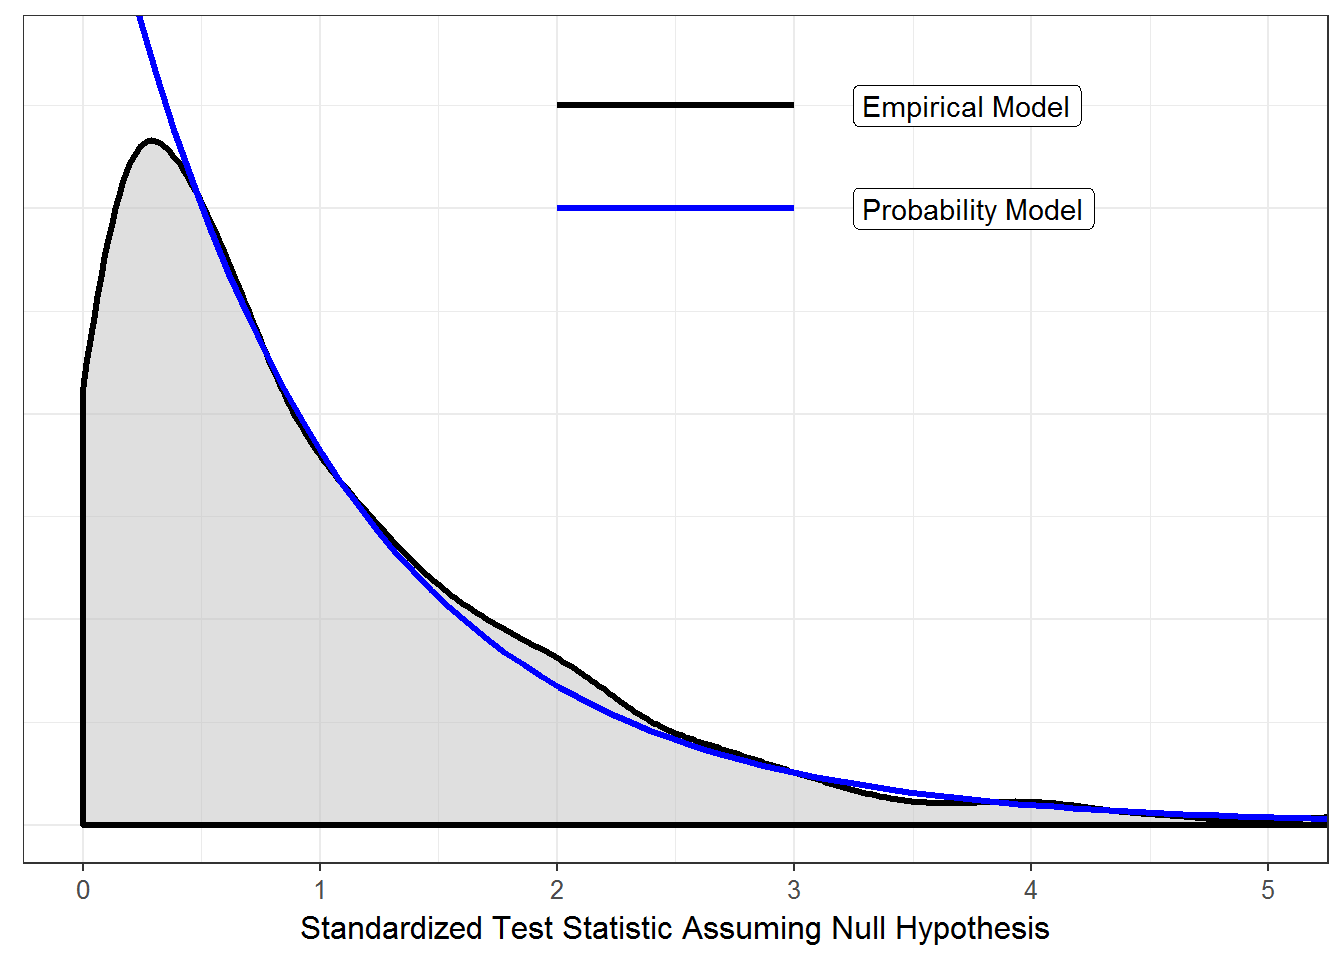
\includegraphics[width=0.8\linewidth]{./Images/anovaclassical-organic-model-1} 

}

\caption{Comparison of the empirical model for the null distribution of our standardized test statistic with the probability model under the classical ANOVA model.}\label{fig:anovaclassical-organic-model}
\end{figure}

Thus, if we are willing to make the assumption that all three conditions
on the error hold, we could rely on the analytical probability model to
compute a p-value instead of the empirical model we get from simulation.
This probability model is called the F-distribution, and as a result,
the standardized test statistic \(T = MSTrt/MSE\) is often referred to
as the F-statistic.

Many software packages contain a function for conducting an analysis
assuming the classicial ANOVA model is valid. When this is the case, the
output has the form in Figure \ref{fig:anovaclassical-table}.

\begin{figure}

{\centering 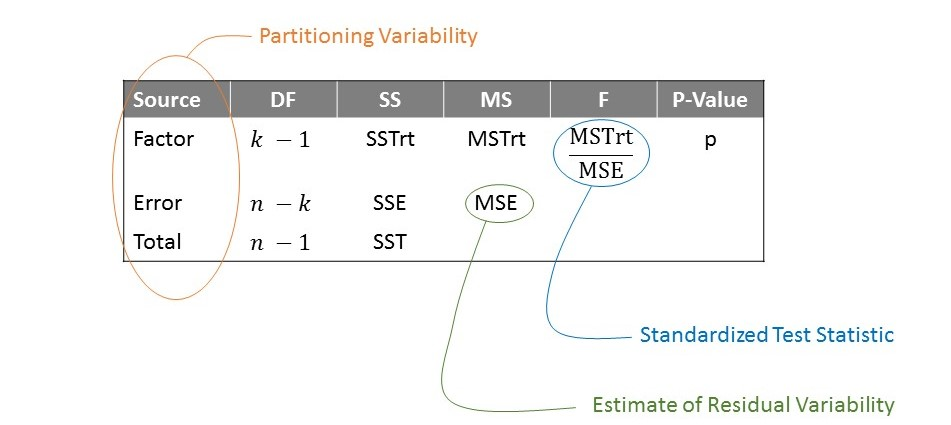
\includegraphics[width=0.8\linewidth]{./images/ANOVAclassical-Table} 

}

\caption{Layout of an ANOVA table which summarizes the analysis conducted.  Emphasis is on partitioning the variability.}\label{fig:anovaclassical-table}
\end{figure}

The table is a way of summarizing the output from the analysis; the
table itself is not very interesting, but we present it because it has
the same emphasis we have in this unit --- partitioning variability. The
key to separating a signal from a noise is to partition the variability
in the data. The total variability is partitioned into that resulting
from the groups (the factor), this is the deterministic portion of the
model that we can explain, and the error, the stochastic portion of the
model that we cannot explain. By partitioning this variability, we are
able to compute the standardized test statistic and the corresponding
p-value. Primarily, the only component we examine in such a table is the
p-value. However, it is worth noting that the mean square for error
(MSE) also provides an estimate of the variance of the errors within a
group, the residual variance. That is, the MSE provides an estimate of
the variance in the response within a group.

\BeginKnitrBlock{rmdtip}
The mean square for error (MSE) is an estimate of the variability in the
response within a particular group.
\EndKnitrBlock{rmdtip}

\section{Analysis of Organic Food Case
Study}\label{analysis-of-organic-food-case-study}

Let's consider the \protect\hyperlink{CaseOrganic}{Organic Food Case
Study} data. We will continue working with the model we have developed
for the moral expectation score:
\[\text{Moral Expectation Score} \sim \text{Food Exposure Group}\]

Further, let's suppose that the data is consistent with all three
classical ANOVA conditions. The results from the corresponding analysis
comparing the average moral expectation score across the three food
conditions are given in Table
\ref{tab:anovaclassical-organic-anova-table}.

\begin{table}

\caption{\label{tab:anovaclassical-organic-anova-table}ANOVA table for the Organic Food Case Study.}
\centering
\begin{tabular}[t]{l|r|r|r|r|r}
\hline
Source & DF & SS & MS & F & P-value\\
\hline
Food Exposure Group & 2 & 0.562 & 0.281 & 0.406 & 0.667\\
\hline
Residuals & 120 & 82.951 & 0.691 &  & \\
\hline
Total & 122 & 83.513 &  &  & \\
\hline
\end{tabular}
\end{table}

As long as the conditions on the error term are reasonable, then we can
interpret the above p-value. Based on these results, there is no
evidence that the moral expectations differ, on average, across the
various food exposure groups. That is, there is no evidence of a
relationship between the type of food to which we are exposed and our
resulting moral expectations, on average.

\section{Recap}\label{recap-1}

By placing an additional condition on the distribution of the error
term, we are able to construct an analytical model for the null
distribution of the standardized test statistic, instead of requiring an
empirical model. Of course, this model for the distribution of the error
terms is an assumption. In fact, we have made several assumptions in
order to compute the p-value given above. It is unwise to place
assumptions on a process without performing some type of assessment to
ensure those assumptions are reasonable --- that the data is consistent
with the assumptions. That is the focus of the next chapter.

\chapter{Assessing Modeling Assumptions}\label{ANOVAassessment}

In the previous chapter, we introduced a model for how a quantitative
response being generated across multiple groups. For the
\protect\hyperlink{CaseOrganic}{Organic Food Case Study}, this is
essentially \[
\text{(Moral Expectation Score)}_i = \sum_{j=1}^3 \mu_j \mathbb{I}(\text{i-th subject in food exposure group j}) + \epsilon_i
\]

Further, we added two conditions to the distribution of the error term:
1. The error in the moral expectation score for one individual is
independent of the error in the moral expectation score for all other
individuals. 2. The variability in the error for the moral expectation
score within a group is similar for any food exposure group.

Unfortunately, we cannot just state that these are the conditions we
hope hold for the data generating process and move on our merry way.
Since the p-value was computed assuming these conditions hold, the
p-value is only meaningful if the data is consistent with these
conditions. If any of these conditions is violated, then the p-value is
meaningless.

\BeginKnitrBlock{rmdkeyidea}
Residuals, since they are estimates of the noise in the data-generating
process, provide a way of assessing the modeling conditions placed on
the distribution of the error term.
\EndKnitrBlock{rmdkeyidea}

In this section, we discuss how to use residuals to assess these
conditions qualitatively.

\section{Assessing Independence}\label{assessing-independence}

Generally, independence is assessed through the context of the data
collection scheme. By carefully considering the manner in which the data
was collected, we can typically determine whether it is reasonable that
the errors in the response are independent of one another. Some key
things to consider when examining the data collection process: - Are
there repeated observations made on the same subject? This often
suggests some type of relationship between the responses and therefore
would not be consistent with errors being independent. - Is the response
measured over time (time-series) such as daily temperature over the
course of a month? Time-series data often exhibits strong
period-to-period relationships suggesting the errors are not
independent. For example, if it is hot today, it will probably be hot
tomorrow as well. - Is there a learning curve in how the data was
collected? Learning curves again suggest some dependence from one
observation to the next.

Random sampling and random assignment allow us to confidently state that
the errors are independent of one another. One additional pitfall to
watch out for when collecting your own data is whether there is some
type of systematic error in the measurement device. - Measurement
devices which are failing over time will introduce a dependence from one
observation to the next. Imagine a bathroom scale that begins to add an
additional pound each day. Then, being above average weight one day will
most likely lead to an above average weight the next, due primarily to
the measurement device.

This last point illustrates a particular deviation from our condition of
independence in which two observations collected close together in time
are related. When we know the order in which the data was collected, we
can assess whether the data is consistent with independence or tends to
deviate in this manner. This is done graphically through a
\textbf{time-series plot} of the \emph{residuals}. If two errors were
unrelated, then the value of one residual should tell us nothing about
the value of the next residual. Therefore, a plot of the residuals over
time should look like noise (since residuals are supposed to be
estimates of noise). If there are any trends, then it suggests the data
is not consistent with independence.

\BeginKnitrBlock{definition}[Time Series Plot]
\protect\hypertarget{def:defn-time-series-plot}{}{\label{def:defn-time-series-plot}
\iffalse (Time Series Plot) \fi{} }Plot of a variable over time. This
plot allows us to assess some deviations from independence. A trend in
the location or spread of the points over time suggests a deviation from
independence.
\EndKnitrBlock{definition}

As an example, consider the time-series plots shown in Figure
\ref{fig:anovaassessment-independence-violations}, both representing
hypothetical datasets. In Panel A, the residuals display a trend in the
location over time. Knowing that a response was below average suggests
the next response will also be below average. In Panel B, the results
deplay a trend in the spread over time. This suggests that measurements
taken later in the study were less precise. Both panels are then
examples of patterns which would suggest the data is not consistent with
the condition of independence.

\begin{figure}

{\centering 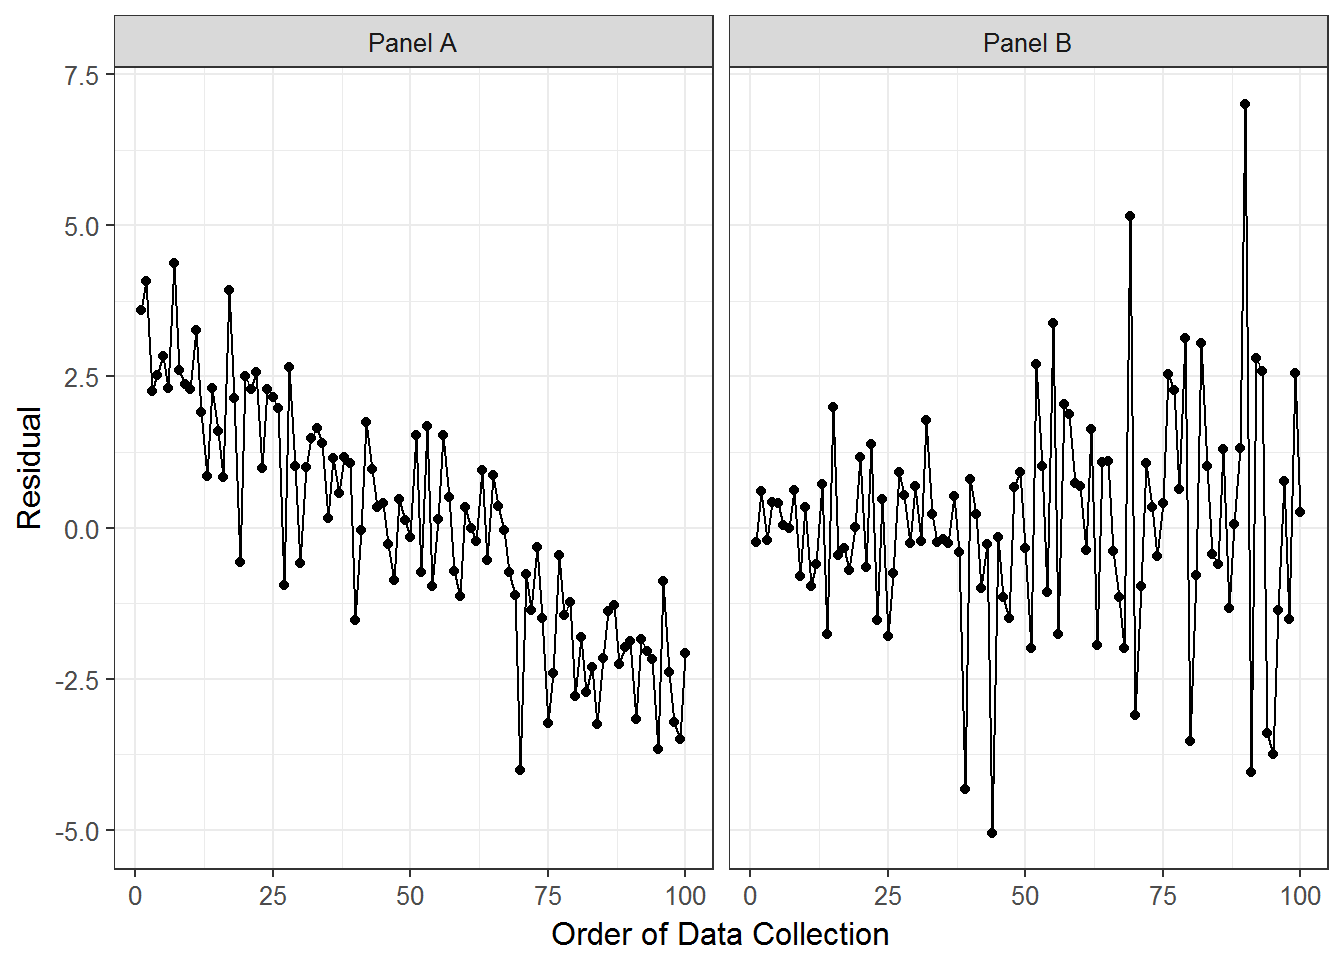
\includegraphics[width=0.8\linewidth]{./Images/anovaassessment-independence-violations-1} 

}

\caption{Examples of trends in a time-series plot of the residuals.  Such trends indicate the data is not consistent with the condition that the errors are independent of one another.}\label{fig:anovaassessment-independence-violations}
\end{figure}

Instead, if the data were consistent with the condition of independence
on the error terms, we would expect to see a plot as in Figure
\ref{fig:anovaassessment-independence-reasonable}. Notice there are no
trends in the location or spread of the residuals.

\begin{figure}

{\centering 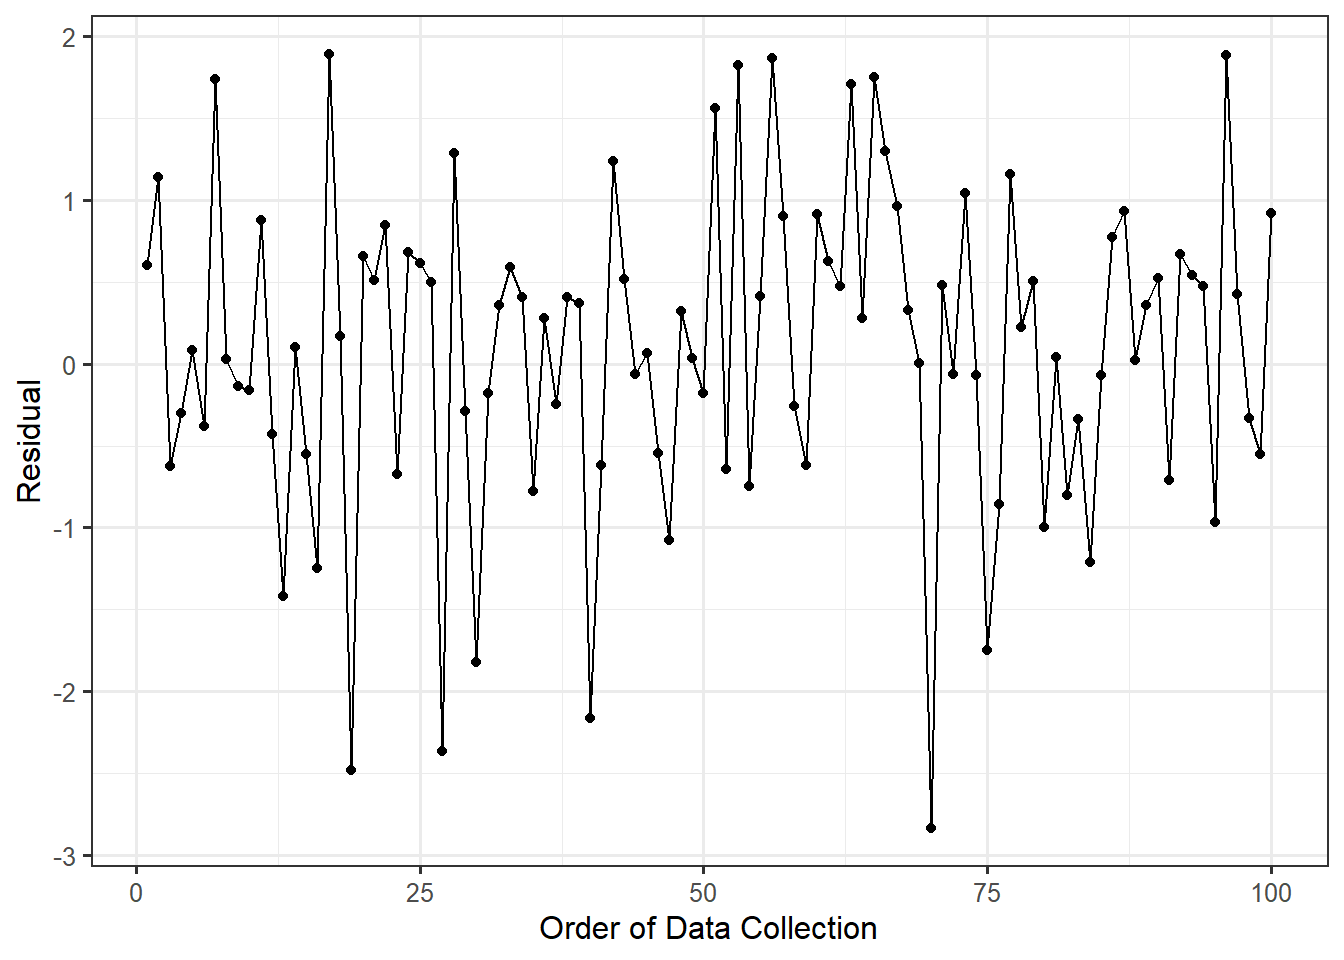
\includegraphics[width=0.8\linewidth]{./Images/anovaassessment-independence-reasonable-1} 

}

\caption{Example of a time-series plot of residuals which shows no trends in location or spread.  This is consistent with what we would expect if the condition of independence among errors were satisfied.}\label{fig:anovaassessment-independence-reasonable}
\end{figure}

For the \protect\hyperlink{CaseOrganic}{Organic Food Case Study},
participants were assessed simultaneously within a large lecture.
Therefore, there is no ordering in time to be concerned about. Further,
since students worked individually on the questionnaire, it is
reasonable to assume that the errors in the moral expectation score are
unrelated to one another.

\section{Assessing Homoskedasticity}\label{assessing-homoskedasticity}

We want the variability in the errors within a group to be the same
across the groups. This corresponds to the spread of the response within
each group is the same. This implication leads to a simple way of
assessing this assumption. Examining the side-by-side boxplots (or
jitter plots, etc.) of the response allows us to get a sense of the
variability within each group. Figure
\ref{fig:anovaassessment-variance-organic} shows the moral expectation
score for each individual across the various groups. Notice that the
boxes for each group are roughly the same size; that is, the
interquartile ranges are similar. This suggests that the variability
within each group is similar from one group to the next. That is, the
data is consistent with this condition.

\begin{figure}

{\centering 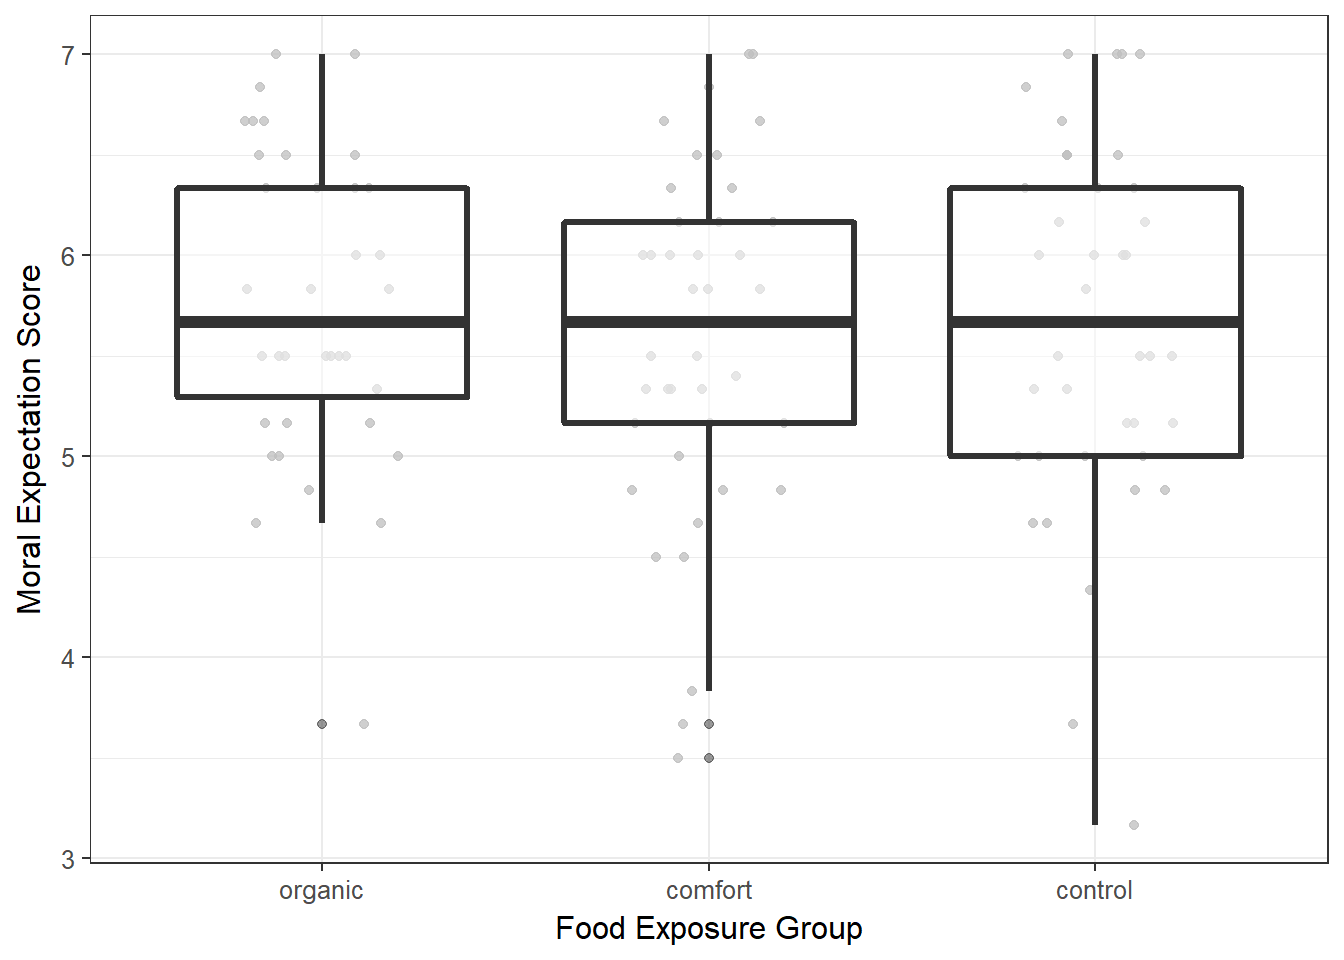
\includegraphics[width=0.8\linewidth]{./Images/anovaassessment-variance-organic-1} 

}

\caption{Comparison of the moral expectations for college students exposed to different types of food.}\label{fig:anovaassessment-variance-organic}
\end{figure}

\section{Assessing Normality}\label{assessing-normality}

Assessing whether observations adhere to a particular distribution is a
large area in statistical research. Many methods have been developed for
this purpose. We emphasize a single graphical summary known as a
\textbf{probability plot}. The construction of the plot is beyond the
scope of this text, but the concepts underlying its construction
actually tie in nicely to the big themes of the course. Recall that if a
sample is representative, then it should be a snapshot of the underlying
population. Therefore, if we believe the underlying population has some
particular distribution, we would expect the properties of this
distribution to be apparent in the sample as well.

If we believe the errors follow a Normal distribution, then it is
reasonable that the residuals should maintain some of those properties.
For example, the 10-th percentile of the residuals should roughly equate
to the 10-th percentile expected from a Normal distribution. Mapping up
the percentiles that we observe to those that we expect is the essence
of a probability plot.

\BeginKnitrBlock{definition}[Probability Plot]
\protect\hypertarget{def:defn-probability-plot}{}{\label{def:defn-probability-plot}
\iffalse (Probability Plot) \fi{} }Graphic for comparing a theoretical
probability model for the distribution an underlying population with the
distribution of the sample. Sample points should follow a straight line.
If points deviate from this linear trend, that suggests the points do
not align with the proposed model.
\EndKnitrBlock{definition}

While a probability plot can be used for a host of probability
distributions, the most common is the normal probability plot. Since we
expect the percentiles to line up directly, we would expect a one-to-one
linear relationship to be exhibited in the plot. Trends away from a
linear relationship suggest the proposed Normal distribution is not a
reasonable model for the distribution of the errors.

Figure \ref{fig:anovaassessment-normal-organic} shows the probability
plot for the residuals from the \protect\hyperlink{CaseOrganic}{Organic
Food Case Study}.

\begin{figure}

{\centering 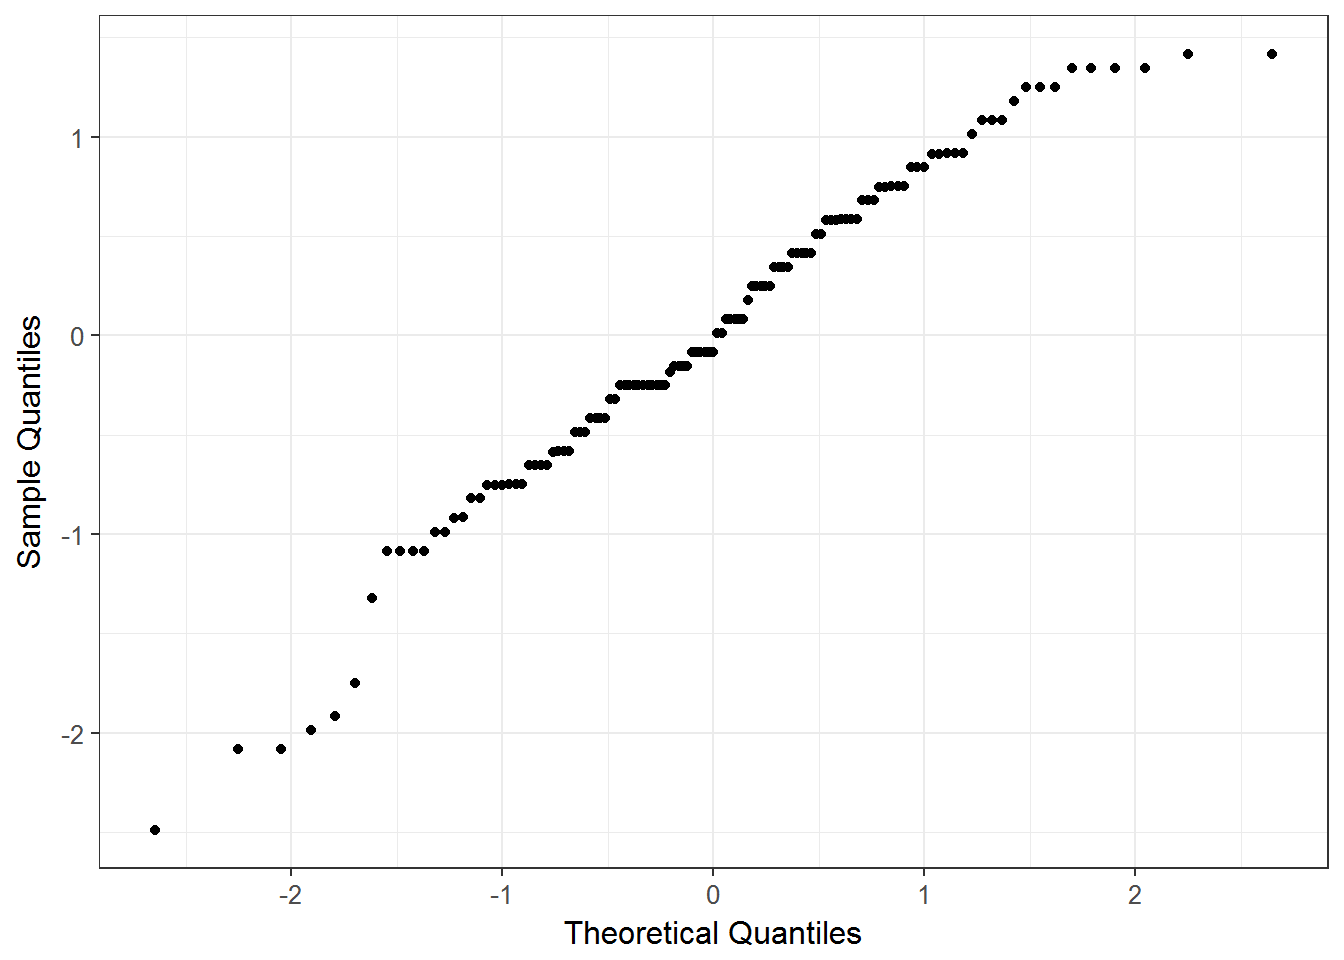
\includegraphics[width=0.8\linewidth]{./Images/anovaassessment-normal-organic-1} 

}

\caption{Probability plot of the residuals for the Organic Food Case Study.  If the errors follow a Normal distribution, we would expect the residuals to fall along a straight line.}\label{fig:anovaassessment-normal-organic}
\end{figure}

Overall, the points do tend to follow a straight line. There are some
deviations from a linear relationship at each end of the plot, but the
deviations are not extreme. We argue that these residuals are consistent
with the errors having a Normal distribution.

For comparison, Figure \ref{fig:anovaassessment-normal-bad} illustrates
a hypothetical dataset for which the residuals suggest the condition of
the errors following a Normal distribution is violated.

\begin{figure}

{\centering 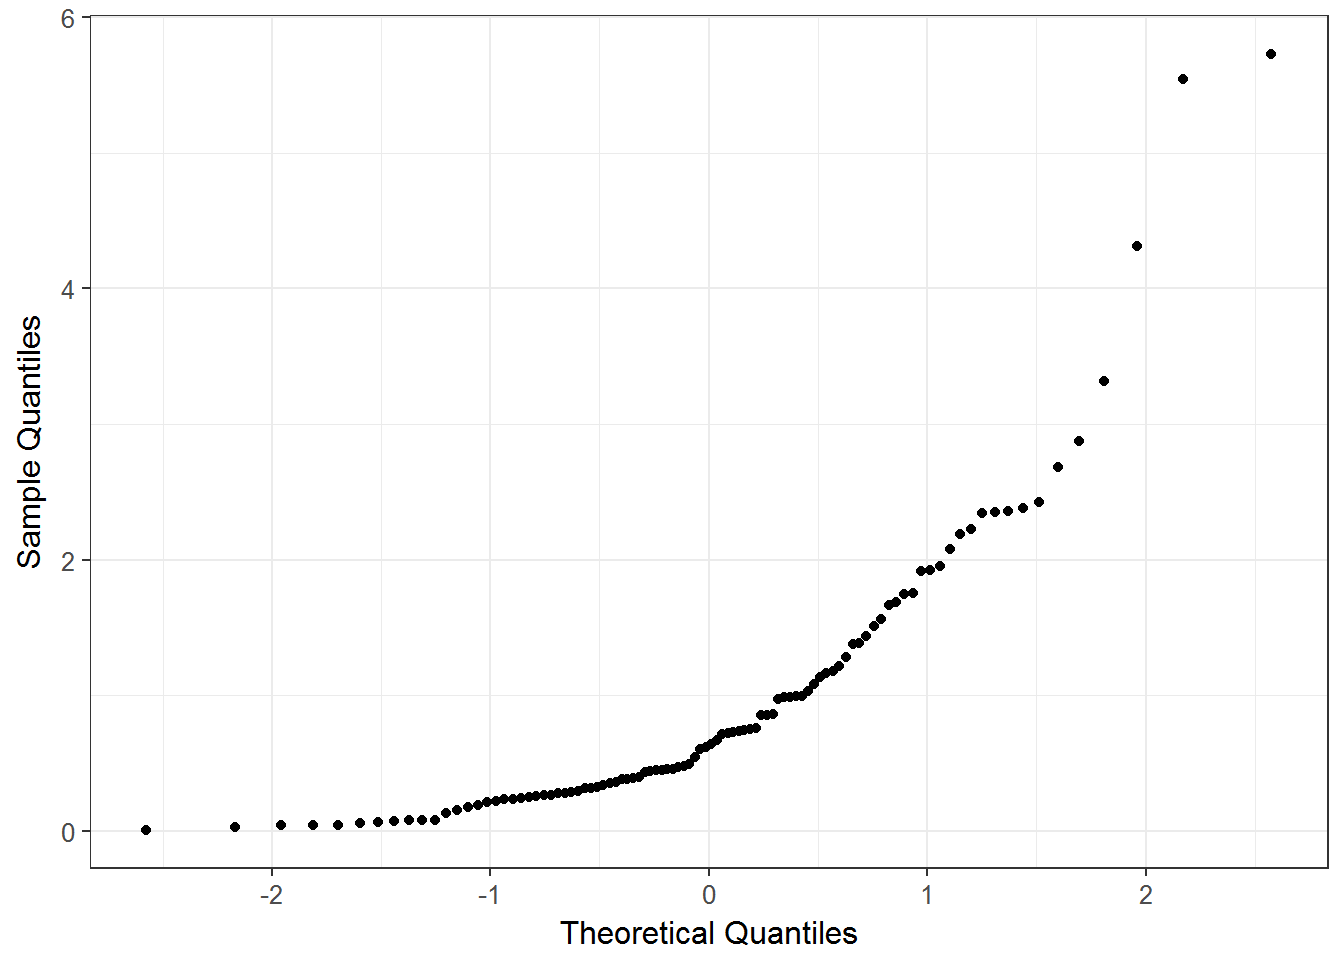
\includegraphics[width=0.8\linewidth]{./Images/anovaassessment-normal-bad-1} 

}

\caption{Probability plot of residuals for a hypothetical dataset.  The trend away from a straight line suggests assuming the errors follow a Normal distribution would be unreasonable.}\label{fig:anovaassessment-normal-bad}
\end{figure}

\section{General Tips for Assessing
Assumptions}\label{general-tips-for-assessing-assumptions}

Each of the methods presented here are qualitative assessements, which
means they are subjective. That is okay. As the analyst, it is up to you
to determine which assumptions you are willing to make. You need to
determine whether you feel the data is consistent with the assumptions.
Here are two overall things to keep in mind.

First, do not spend too much time examining residual plots. If you stare
at a plot too long, you can convince yourself there is pattern in
anything. We are looking for glaring evidence that the data is not
consistent with the conditions we have imposed on our model. This is
especially true when we have only a few observations. In these settings,
reading plots can be very difficult. Again, it is about what you are
comfortable assuming; how much faith do you want to place in the
results?

Second, we have chosen the language carefully throughout this chapter.
We have never once stated that a condition was satisfied. When we
perform an analysis, we are making an assumption that the conditions are
satisfied. We can never prove that they are; we can only show that the
data is consistent with a particular condition. We can, however, provide
evidence that a condition is violated. When that is the case, we should
be wary of trusting the resulting p-values and confidence intervals.
This is not unlike hypothesis testing; just as we can never prove the
null hypothesis is true, we cannot prove that a condition is satisfied.

Finally, any conditions required for a particular analysis should be
assessed. If your sample is not consistent with the necessary
conditions, you should choose a different analysis. The inference you
obtain from an analysis is only reliable of the data is consistent with
any necessary conditions.

\BeginKnitrBlock{rmdtip}
The conditions for a model are placed on the error, but the residuals
are used to assess whether a dataset is consistent with these
conditions, allowing us to determine if assuming the conditions are
satisfied is reasonable.

\begin{enumerate}
\def\labelenumi{\arabic{enumi}.}
\tightlist
\item
  We can never prove a condition is satisfied.
\item
  The assumptions are not on the residuals, but the errors.
\item
  A sample should be consistent with any conditions you impose on your
  model.
\end{enumerate}

If a sample is not consistent with the conditions you impose, you should
consider revising your analysis.
\EndKnitrBlock{rmdtip}

\chapter{Using the Tools Together}\label{ANOVArecap}

This unit introduced a framework for determining if there is an
association between a quantitative response and a categorical predictor.
We formed a standardized test statistic for measuring the signal, and
then we developed a model for the data-generating process which allowed
us to model the null distribution of the standardized statistic. In this
chapter, we pull these tools together once more to answer a research
question.

The primary question we have been addressing in this unit was whether
the moral expectations of students were affected by the type of food to
which they were exposed. We saw that there was little evidence of a
relationship between these two variables. We now use the data from the
\protect\hyperlink{CaseOrganic}{Organic Food Case Study} to answer a
related question:

\begin{quote}
Do the moral expectations of males and females differ?
\end{quote}

\section{Framing the Question (Fundamental Idea
I)}\label{framing-the-question-fundamental-idea-i-1}

As stated, the above question is ill-posed. We have not identified a
variable or parameter of interest. We refine this question to be

\begin{quote}
Does the average moral expectation score of males differ from that of
females?
\end{quote}

This question could also be stated as the following set of hypotheses:

\begin{quote}
Let \(\mu_1\) and \(\mu_2\) represent the average moral expectation
score for males and females, respectively.\\
\(H_0: \mu_1 = \mu_2\)\\
\(H_1: \mu_1 \neq \mu_2\)
\end{quote}

\section{Getting Good Data (Fundamental Idea
II)}\label{getting-good-data-fundamental-idea-ii-1}

As we are working with previously collected data, our goal in this
discussion is not how best to collect the data but making note of the
limitations of the data as a result of how it was collected. We
previously described the \protect\hyperlink{CaseOrganic}{Organic Food
Case Study} as an example of a controlled experiment. This was
true\ldots{}with regard to the primary question of interest (moral
expectations and food exposure). However, the subjects were \emph{not}
randomly assigned to gender here; therefore, with regard to this
question of interest, the data was an observational study.

It is common for young researchers to believe that if initially a
controlled experiment was performed that the data always permits a
causal interpretation. However, we must always examine the data
collection with respect to the question of interest. Such ``secondary
analyses'' (using data collected from a study to answer a question for
which the data was not initially collected) are generally observational
studies. As a result, there may be other factors related to gender and
moral expectations that drive any results we may see.

\section{Presenting the Data (Fundamental Idea
III)}\label{presenting-the-data-fundamental-idea-iii-1}

Our question here is examining the relationship between a quantitative
response (moral expectation score) and a categorical predictor (gender).
Figure \ref{fig:anovarecap-boxplot} compares the distribution of the
moral expectation score for the two groups. Note that 4 students did not
specify their gender; these subjects will be removed from the analysis.

\begin{figure}

{\centering 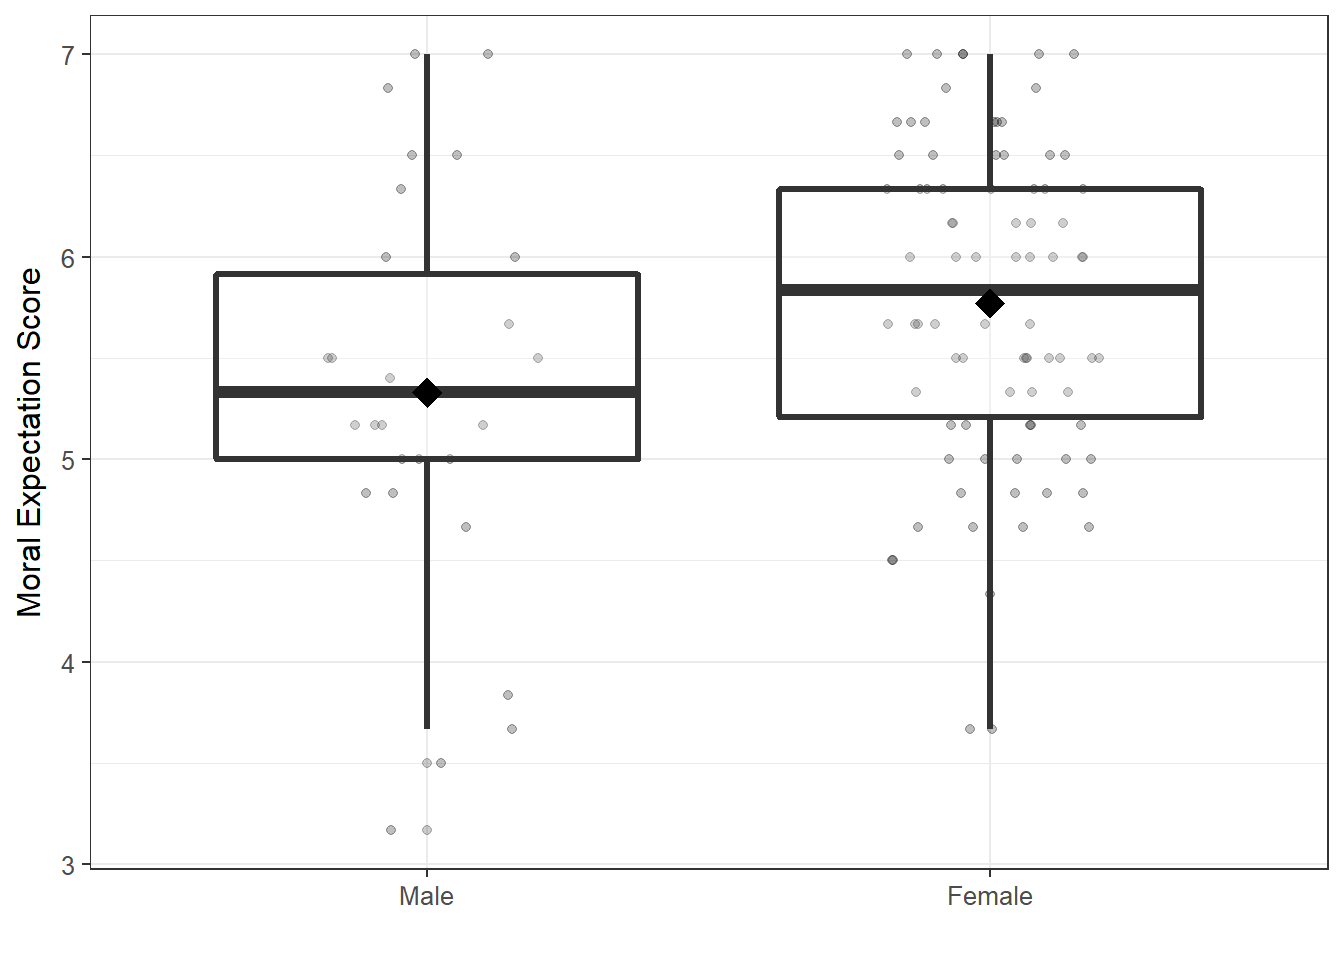
\includegraphics[width=0.8\linewidth]{./Images/anovarecap-boxplot-1} 

}

\caption{Comparison of the moral expectations of males and females. The average value is added for each group.  Students who did not specify their gender were removed from the analysis.}\label{fig:anovarecap-boxplot}
\end{figure}

Based on the above graphic, it appears the females tend to have higher
moral expectations by about 1 point, compared to males. We also observe
that there are many more females in our sample compared to males, which
is probably a result of the type of class and the demographic makeup of
the university at which the study was conducted.

\section{Quantifying the Variability in the Estimate (Fundamental Idea
IV)}\label{quantifying-the-variability-in-the-estimate-fundamental-idea-iv-1}

In order to measure the size of the signal, we can compute the
standardized test statistic \[T = \frac{MSTrt}{MSE}\]

which is 6.52 for the sample we have observed. Of course, if we were to
collect a new sample, we would expect this value to change. If we want
to quantify the variability in this statistic, we need a model for its
sampling distribution. More, what we are really interested in is the
sampling distribution of this statistic if the average moral expectation
score were the same for the two genders; that is, we are interested in
the null distribution of this standardized test statistic. With the null
distribution, we could ascertain how unlikely (how strong the evidence)
our sample is.

In order to model the null distribution, we consider the following model
for the data-generating process:
\[\text{Moral Expectation Score} \sim \text{Gender}\] Formally, we write

\begin{equation}
  \begin{split}
    (\text{Moral Expectation Score})_i & = \mu_1\mathbb{I}(\text{i-th subject is a male}) \\
      & \quad + \mu_2\mathbb{I}(\text{i-th subject is a female}) + \epsilon_i
  \end{split}
  \label{eq:anovarecap-model}
\end{equation}

where we make the following assumptions on the error term:

\begin{enumerate}
\def\labelenumi{\arabic{enumi}.}
\tightlist
\item
  The error in the moral expectation score for one individual is
  independent of the error in the moral expectation score for any other
  individual.
\item
  The variance of the error in the moral expectation scores for males is
  the same as the variance of the error in moral expectation scores for
  females.
\item
  The error in the moral expectation score for individuals follows a
  Normal Distribution.
\end{enumerate}

Under these three assumptions, we are able to construct a model for the
null distribution of the standardized test statistic. Figure
\ref{fig:anovarecap-classical-null-model} illustrates the null
distribution assuming these conditions are satisfied.

\begin{figure}

{\centering 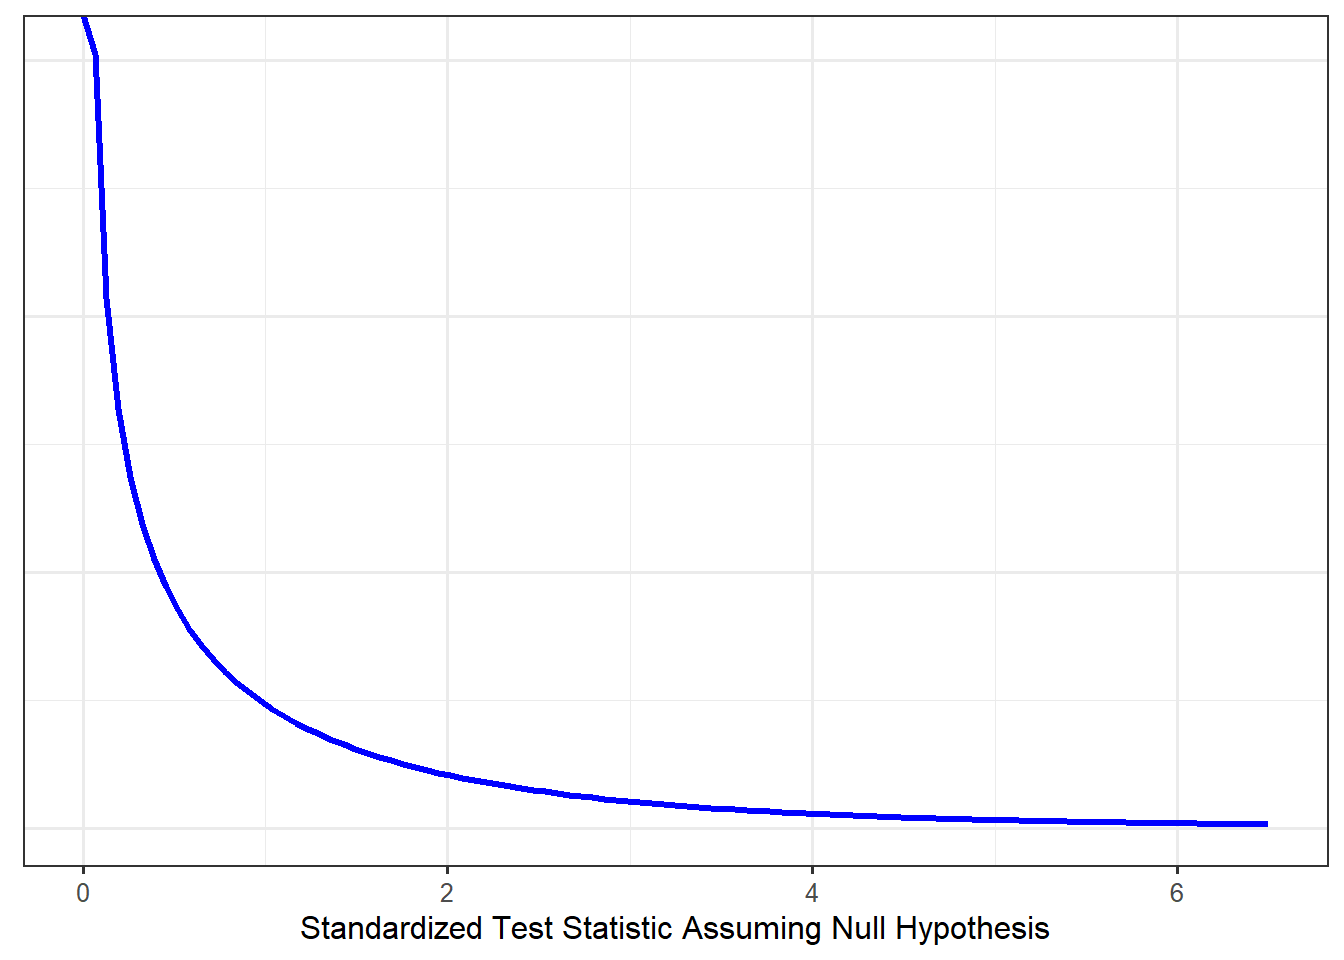
\includegraphics[width=0.8\linewidth]{./Images/anovarecap-classical-null-model-1} 

}

\caption{Model for the standardized test statistic measuring the signal comparing the moral expectation scores for males and females in the Organic Food Case Study.  This model is constructed assuming the classical ANOVA conditions are satisfied.}\label{fig:anovarecap-classical-null-model}
\end{figure}

Before we can use this model to make any conclusions regarding our
question of interest, we need to address the fact that we have assumed
certain conditions are satisfied. We need to assess whether the data is
consistent with these assumptions. This requires examining the residuals
for the model. That is, we must determine how far away the moral
expectation score for each individual is from the average moral
expectation score for their group.

First, we discuss the assumption of independence. Since the data was
collected at a single point in time, known as a \emph{cross-sectional
study}, constructing a time-series plot of the residuals would not
provide any information regarding this assumption. Instead, we rely on
the context of the problem to make some statements regarding whether the
data is consistent with this condition (whether making this assumption
is reasonable). It is reasonable that whether a student has a slightly
above (or below) moral expectation score is not related to whether any
other student has a slightly above (or below) moral expectation score.
That is, it is reasonable that the errors are independent. One case in
which this might be violated is if students discussed their answers to
the questions as they filled out the survey; then, it is plausible that
one student influenced another's responses. As this is unlikely given
the description of the data collection, we feel it is reasonable to
assume independence.

Again, note that there is a condition of independence; we are simply
saying whether we are willing to assume the condition is satisfied.
There is no way to ensure a condition holds.

In order to assess the condition of constant variance, let us look back
at the box plots given in Figure \ref{fig:anovarecap-boxplot}. As the
spread of the moral expectation score for each of the two genders is
roughly the same, it is reasonable to assume the variability of the
errors in each group is the same.

Finally, to assess the condition that the distribution of the errors is
Normal, we consider a probability plot of the residuals (Figure
\ref{fig:anovarecap-resids-probplot}). Given that the residuals tend to
display a linear relationship, it is reasonable that the residuals
represent a sample from a Normal Distribution. That is, it is reasonable
that the errors follow a Normal Distribution.

\begin{figure}

{\centering 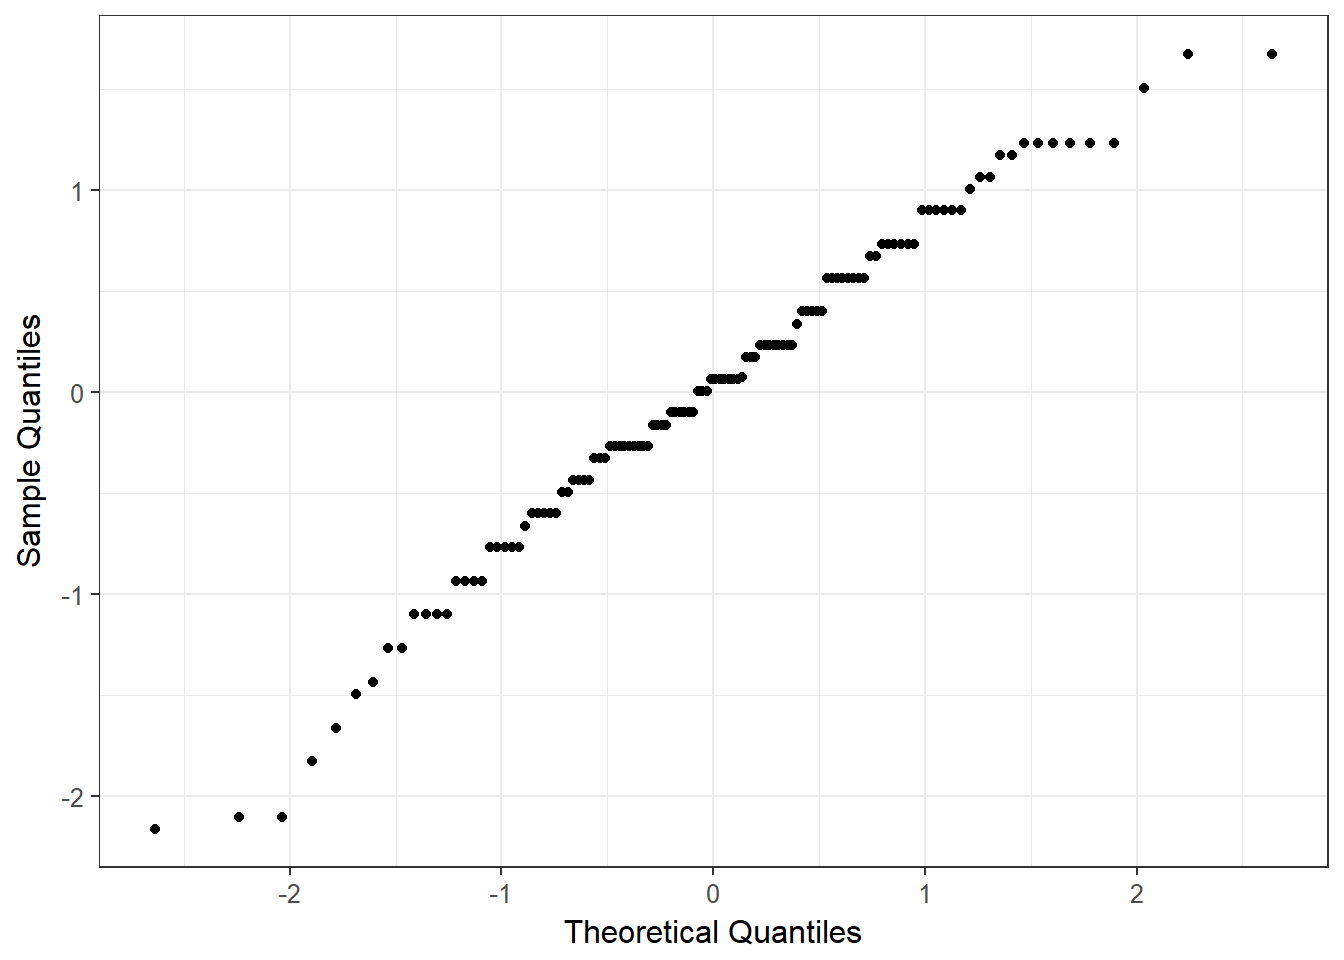
\includegraphics[width=0.8\linewidth]{./Images/anovarecap-resids-probplot-1} 

}

\caption{Probability plot assessing the assumption that the errors for our model comparing the moral expectation score across gender follow a Normal Distribution.}\label{fig:anovarecap-resids-probplot}
\end{figure}

Given that we are comfortable assuming the conditions on the error term
are reasonable, we can make use of the analytical model for the null
distribution in Figure \ref{fig:anovarecap-classical-null-model}.

\section{Quantifying the Evidence (Fundamental Idea
V)}\label{quantifying-the-evidence-fundamental-idea-v-1}

Now that we have a model for the null distribution, we can determine how
extreme our particular sample was by comparing the standardized test
statistic for our sample with this null distribution. We can measure
this through computation of a p-value, the probability that we would
observe a standardized test statistic of this magnitude or higher by
chance alone if there were no difference in the mean moral expecation
scores of males and females. This is summarized in Table
\ref{tab:anovarecap-anova-table} below.

\begin{table}

\caption{\label{tab:anovarecap-anova-table}ANOVA table summarizing the comparison of the moral expectation score across gender within the Organic Food Case Study.}
\centering
\begin{tabular}[t]{l|r|r|r|r|r}
\hline
Source & DF & SS & MS & F & P-value\\
\hline
Gender & 1 & 4.363 & 4.363 & 6.517 & 0.012\\
\hline
Residuals & 118 & 79.008 & 0.670 &  & \\
\hline
Total & 119 & 83.372 &  &  & \\
\hline
\end{tabular}
\end{table}

Based on the plot of the null distribution above, we should have
expected a small p-value since hardly any of the standardized statistics
exceeded the 6.517 we observed in our sample. From the results, we can
conclude that there is evidence (p = 0.012) of a relationship between
the moral expectations of a student and their gender. Looking back at
Figure \ref{fig:anovarecap-boxplot}, females tend to have higher moral
expectations.

\section{Conclusion}\label{conclusion}

Throughout this unit, we have examined a framework for examining the
association between a quantitative response and a categorical predictor.
This served to introduce a couple of big ideas we will make use of
throughout the remainder of this text:

\begin{itemize}
\tightlist
\item
  The key to measuring a signal is to partition the variability in the
  response.
\item
  A standardized test statistic is a numeric measure of the signal
  strength in the sample.
\item
  Modeling the data-generating process provides us a way of modeling the
  sampling distribution and null distribution of a standardized
  statistic.
\item
  Conditions are often placed on the noise portion of the model for the
  data-generating process; before assuming these conditions are met, we
  should graphically assess whether the data is consistent with these
  conditions.
\end{itemize}

Within this unit, we focused on a categorical predictor. In the next
unit, we consider the case when we have a quantitative predictor or even
a collection of predictors.

\chapter{Analyzing a Design that Incorporates
Blocking}\label{ANOVAblocking}

In Chapter \ref{ANOVAdata} we discussed various characteristics of a
good study design. Prior to this chapter, the study design has
influenced the interpretations of the results (can we assume cause and
effect, for example) but not the analysis itself. That is, whether the
data is from an observational study or a controlled experiment, we used
a model of the form \[\text{Response} \sim \text{Factor}\]

where we had a quantitative response and a categorical predictor (or
factor). However, it is not always the case where the study design and
the analysis are unrelated. When we incorporate blocking into the study
design, it has major implications with regard to the study. This chapter
explores those implications.

\section{What is the Big Deal?}\label{what-is-the-big-deal}

Why does blocking impact our analysis. Consider Example
\ref{ex:anova-golf} from Chapter \ref{ANOVAdata}; briefly, a study was
conducted to determine if the type of seed used on a golf green has an
effect on the distance a ball rolls on the green. This appears to fit
into the framework we have been discussing in this unit --- we have a
quantitative response (the distance the ball rolls) and a categorical
predictor (the type of seed used on the green). Therefore, we might
suggest the following model:
\[\text{Rolling Distance} \sim \text{Seed Variety}\]

Formally, we have that
\[(\text{Rolling Distance})_i = \sum_{j=1}^{5} \mu_j \mathbb{I}(\text{i-th ball rolled on green seeded with variety j}) + \epsilon_i\]

Further, we might assume the following conditions on the distribution of
the error term:

\begin{enumerate}
\def\labelenumi{\arabic{enumi}.}
\tightlist
\item
  The error in the distance one ball rolls is independent of the error
  in the distance of any other ball.
\item
  The variance of the error in the distance a ball rolls is similar for
  all five seed varieties.
\item
  The error in the distance a ball rolls follows a Normal Distribution.
\end{enumerate}

The problem now arises. The errors cannot possibly be independent; in
fact, we purposely designed a study in which that was not the case!
Remember the goal of blocking is to group subjects which are alike with
respect to some inherent characteristic. In our example here, the greens
with a similar slope were grouped together and the randomization of a
green to a particular seeding variety occured within each block (group
of greens with similar slope). That is, we recognized that the way a
ball rolls within these greens is quite similar. So, if the ball rolls a
little further on average on a green with a steep slope, then we can
expect that it will roll a little further on average for most greens
within that same slope block. This suggests the errors in the rolling
distance are not independent.

Since the data is not consistent with the conditions we have placed on
the model, we are unable to conduct the same types of analyses
(classical or resampling-based) presented in the prior chapters. We need
a new strategy.

\section{Solution: Partition the
Variability}\label{solution-partition-the-variability}

We have seen throughout this unit that the key to measuring a signal is
to partition the sources of variability that contribute to the response.
Again, this is best explained through a graphic. Figure
\ref{fig:anovablocking-golf-raw} presents the rolling distance of the
golf balls on the various greens.

\begin{figure}

{\centering \includegraphics[width=0.8\linewidth]{./Images/anovablocking-golf-raw-1} 

}

\caption{Comparison of the rolling distance of golf balls seeded with one of five types of Rye grass.  Greens with similar slopes were grouped prior to randomization.  The slope groups, of which there are 4, are denoted by a common value.}\label{fig:anovablocking-golf-raw}
\end{figure}

Even the way we present the data must account for the relationship
present in the observed responses. Greens which belong to a similar
group are indicated on the graphic. We see that balls rolled on those
greens in group 3 tended to travel less distance, compared to balls on
other greens. However, for all groups, the ball tended to roll the
furthest when seeded with Variety A.

This discussion helps to tease out the sources of variability:

\begin{itemize}
\tightlist
\item
  Type of Rye Seed: the distance the ball rolled is potentially related
  to the type of Rye grass used on the green. That is, we might expect
  the distance to be different as we move from one variety to another.
  This is reflected in our primary question.
\item
  Slope of Green: the slope of the green will affect the distance the
  ball travels. As a result, greens were grouped. Therefore, the group
  to which the green belongs also contributes to the variability in the
  distance the ball rolls. While we would like to address this, it is
  not primarily part of our research question; this is a nuisance
  variable.
\item
  Error in the Process: balls do not always roll the same distance, even
  on two greens within the same slope group and assigned to the same Rye
  variety. This is the variability we cannot explain. It is also a
  nuisance.
\end{itemize}

The first and third sources of variability mentioned above are what we
have been discussing throughout this unit. The second source of
variability is a result of the blocked design. The solution to our
modeling problem is to simply incorporate this additional component of
the variability. As we will see in the next unit, this is a general
modeling strategy --- whenever we have additional information which
contributes to why there is variability in the response, we incorporate
that information into our model. What is unique here is that we are not
particularly interested in the slope of the green; it is a nuisance.
That is, we are not interested in determining which variety of Rye we
should place on a green with a particular slope; we actually believe
there is probably one superior type of seed regardless of the slope.
Placing the greens into groups was simply to reduce this additional
variability. The fact that the slope group is a nuisance, similar to the
overall noise in the data generating process, gives us an idea on how we
approach this in our model.

Our overall model is still
\[\text{Rolling Distance} \sim \text{Seed Variety}\]

However, we now need to partition the noise a bit further when we
formally write the model; this leads to \[
\begin{aligned}
  (\text{Rolling Distance})_i &= \sum_{j=1}^{5} \mu_j \mathbb{I}(\text{i-th ball rolled on green seeded with variety j}) \\
    &\quad + \sum_{k=1}^{4} \alpha_k\mathbb{I}(\text{i-th ball rolled on green belonging to slope group k}) \\
    &\quad + \epsilon_i
\end{aligned}
\]

We have essentially added an additional set of noise terms
\(\alpha_1, \dotsc, \alpha_4\) which capture the additional ``bump'' we
should expect to the distance the ball rolls as a result of being in a
particular slope group. Now, we can place certain conditions on each of
these error terms; for example,

\begin{itemize}
\tightlist
\item
  The bump to the rolling distance is the same for all balls within the
  same slope group.
\item
  The bump to the rolling distance for a ball in one group is
  independent of the bump to the rolling distance for a ball in any
  other group.
\item
  The bumps to the rolling distance across groups follows a Normal
  Distribution.
\item
  The error in the rolling distance for one ball within a slope group is
  independent of the error in the rolling distance for a ball within the
  same slope group.
\item
  The error in the rolling distance for balls within the same slope
  group is similar across all seeding varieties.
\item
  The error in the rolling distance follows a Normal Distribution.
\item
  The error in the rolling distance is independent of the bump that
  occurs to a ball for being from a particular slope group.
\end{itemize}

Many of these additional conditions (those placed on the ``bumps'')
cannot be assessed. Instead, we determine based on the context of the
problem whether we feel these assumptions are reasonable. Further
investigation of the details of this model and its conditions is beyond
the scope of this course. We focus on the interpretation of the
resulting output.

\section{Interpreting the Analysis}\label{interpreting-the-analysis}

The resulting output looks similar to what we have seen previously
(Table @ref); the only change is that the variability now includes an
additional component to the partition. As this additional component was
a nuisance, we refrain from making any interpretations from this
component. We focus instead on the component of interest: the
variability due to the factor.

\begin{table}

\caption{\label{tab:anovablocking-anova-table}ANOVA table summarizing the comparison of the ball roll for different seeding varieties while accounting for the slope of the green.}
\centering
\begin{tabular}[t]{l|r|r|r|r|r}
\hline
Source & DF & SS & MS & F & P-value\\
\hline
Rye Seed Variety & 4 & 0.452 & 0.113 & 8.345 & 0.002\\
\hline
Slope Group & 3 & 1.051 & 0.350 & 25.867 & 0.000\\
\hline
Residuals & 12 & 0.163 & 0.014 &  & \\
\hline
Total & 19 & 1.666 &  &  & \\
\hline
\end{tabular}
\end{table}

From the analysis, we have strong evidence (p = 0.002) that the distance
a ball rolls, on average, is associated with the type of Rye grass used
on the green. From our initial graphical summary of the data, if you
would like a course which has fast greens, we would recommend seeding
with Variety A.

\part{Unit III: Modeling the Average Response as a Function
of Several
Predictors}\label{part-unit-iii-modeling-the-average-response-as-a-function-of-several-predictors}

\hypertarget{CaseGreece}{\chapter{Case Study: Seismic Activity in
Greece}\label{CaseGreece}}

At the intersection of the African plate, the Eurasia plate, and the
smaller Aegean plate, Greece is one of the most earthquake-prone regions
in the world. Between July 2016 and July 2017, Greece experienced 179
earthquakes; by contrast, the state of Texas experienced 28 over the
same span of time. In a region with such seismic activity, careful
consideration must be given to municipal construction. Further,
understanding how the motion experienced in a location is related to the
soil properties in the area or the magnitude and distance of an
earthquake is important.

An article in the \emph{Journal of Earthquake Engineering} (Koutrakis et
al. \protect\hyperlink{ref-Koutrakis2002}{2002}) examined seismic events
in Greece occurring between 1978 and 1997. Of interest for construction
is characterizing the ``strong ground motion,'' when the earth shakes
with enough force to cause damage to infrastructure, with respect to the
properties of a location. The study recorded several measurements from
121 stations (representing 93 distinct seismic events)\footnote{The
  original article presented repeated measurements at each location. We
  present here only the first measurement from each location to simplify
  any analyses. Repeated measurements are discussed briefly later in the
  text; for a more thorough treatment of the subject, we recommend a
  course in Designed Experiments or Biostatistics. The dataset presented
  here corresponds to that presented in Navidi's ``Statistics for
  Engineers and Scientists'' (Chapter 8, Supplementary Exercise 22).}.
The primary variable of interest is the \emph{bracketed duration}, ``the
time interval {[}in seconds{]} between the first and last excursion of
the peak ground acceleration beyond a certain predefined level.'' For
our purposes, we only consider the data corresponding to a threshold of
2\% of the acceleration due to gravity. In addition, the following
measurements were available for each observation:

\begin{itemize}
\tightlist
\item
  Moment Magnitude: a measure of the size of the earthquake; larger
  values indicate more severe earthquakes.
\item
  Epicentral Distance: distance (kilometers) from the epicenter of the
  earthquake to the location at which the measurement was taken.
\item
  Soil Condition: indicator of the type of soil present at the
  measurement site. Soil was categorized as one of three types -
  alluvium (soft, fine particles of clay, silt, sand, and gravel),
  intermediate soil conditions, or tertiary or older rock (those older
  than 2.58 million years).
\end{itemize}

The first 5 observations in the dataset are shown in Table
\ref{tab:casegreece-table}. We are interested in characterizing the
relationship between bracketed duration and the magnitude of the
earthquake.

\begin{table}

\caption{\label{tab:casegreece-table}Data for first 5 observations from study characterizing seismic activity in Greece.}
\centering
\begin{tabular}[t]{r|r|r|l}
\hline
Magnitude & Distance from Epicenter (km) & Bracketed Duration (s) & Soil Conditions\\
\hline
6.4 & 30 & 8.82 & Soft\\
\hline
5.3 & 6 & 4.31 & Intermediate\\
\hline
5.6 & 15 & 5.74 & Intermediate\\
\hline
5.2 & 7 & 4.08 & Intermediate\\
\hline
6.6 & 31 & 28.27 & Soft\\
\hline
\end{tabular}
\end{table}

\chapter{Myriad of Potential Questions}\label{Regquestions}

For the \protect\hyperlink{CaseGreece}{Seismic Activity Case Study}, we
are primarily interested in characterizing the relationship between
bracketed duration and the magnitude of the earthquake. First, note that
this question is about the relationship between a quantitative response
(bracketed duration; see Definition \ref{def:defn-response}) and a
quantitative predictor (magnitude). Also note that the question is quite
broad. We might actually have one of the following more specific ideas
in mind:

\begin{itemize}
\tightlist
\item
  In general, does the bracketed duration increase as the magnitude
  increases?
\item
  If two earthquakes with different magnitudes occur in the same
  location, would we expect the same bracketed duration regardless of
  their magnitudes?
\item
  Is the relationship between the bracketed distance and the magnitude
  different depending on the soil condition of where the measurement is
  taken?
\end{itemize}

These questions illustrate an array of potential questions we address in
this unit. In fact, each represents a different emphasis that we might
have in a research question:

\begin{itemize}
\tightlist
\item
  Marginal Relationship: overall, do two variables tend to move together
  (are they correlated)?
\item
  Isolation of Effect: does a relationship exist after accounting for
  the effect of additional variables? Or, what is the effect ``above and
  beyond'' the effect of additional variables?
\item
  Interplay: how does the relationship between two variables change as a
  result of a third?
\end{itemize}

There is no right question to ask; each question examines a different
facet of the relationship between two quantitative variables. Throughout
this unit, we will introduce a framework which is broad enough for
addressing each of these types of questions. This may sound daunting,
but keep in mind that the fundamental ideas we discussed in Units I and
II will continue to form the foundation of the analyses introduced in
this unit; namely,

\begin{itemize}
\tightlist
\item
  We are using a sample to say something about the underlying
  population.
\item
  In order to make inference, we will need a model for the sampling (or
  null) distribution of our statistic.
\item
  In order to form a statistic of interest which measures the strength
  of the signal in the dataset, we think about partitioning variability.
\end{itemize}

The ideas remain the same; the context has changed. Stating these
questions mathematically will require us to build a model for the
data-generating process, which we will examine in an upcoming chapter.

There is one more thing we want to point out before moving on: any
relationships we observe are overall trends, not guaranteed to hold for
any single individual. Recall that in Unit II we emphasized that our
conclusions were about the mean response within each group (the
parameter of interest). Specifically, even if one treatment is found to
be superior \emph{on average} within the population, due to variability,
we do not expect the treatment to necessarily be superior for every
individual. The effect was an overall trend. This will continue in this
unit. If we observe, for example, that an increase in the magnitude is
associated with an increase in the bracketed duration, we are describing
an overall trend. It is highly likely there is some location for which
this trend does not hold, simply due to variability.

\chapter{Nature of Collecting Multivariable Data}\label{Regdata}

For the \protect\hyperlink{CaseGreece}{Seismic Activity Case Study}, we
are primarily interested in characterizing the relationship between
bracketed duration and the magnitude of the earthquake. As we discussed
in the previous chapter, this general goal might be refined into one of
many specific questions:

\begin{itemize}
\tightlist
\item
  In general, does the bracketed duration increase as the magnitude
  increases?
\item
  If two earthquakes with different magnitudes occur in the same
  location, would we expect the same bracketed duration regardless of
  their magnitudes?
\item
  Is the relationship between the bracketed distance and the magnitude
  different depending on the soil condition of where the measurement is
  taken?
\end{itemize}

Notice that these last two questions actually require knowledge of more
than just the braketed duration and the magnitude of each seismic event.
In order to address the second question, we would also need the distance
from the center of the earthquake; in order to address the third
question, we also need the soil conditions of where the measurement is
taken. Often, research questions require knowledge of more than just two
variables; such questions are \textbf{multivariable}.

\BeginKnitrBlock{definition}[Multivariable]
\protect\hypertarget{def:defn-multivariable}{}{\label{def:defn-multivariable}
\iffalse (Multivariable) \fi{} }Refers to questions of interest which
involve more than a single variable. Often, these questions involve many
variables.
\EndKnitrBlock{definition}

Consider going to the doctor because you are feeling ill. The doctor
does not have you simply enter your most prominent symptom (fever, for
example) into a computer and then prescribe a medication based solely on
that single symptom. Instead, a good physician will review all symptoms
you are experiencing, as well as your medical history, other
medications, allergies, etc. The physician operates in a multivariable
world in which there are many contributing factors to a response.
Therefore, when you arrive for this hypothetical visit, they record
several variables which may be of interest.

Studies which collect several variables can be observational studies or
controlled experiments. If an observational study, we ensure the sample
of subjects is representative of the population. Then, for each
individual, we simply record several variables. If a controlled
experiment, we would randomly assign subjects to a particular group;
afterwards, we would measure the response in addition to other
variables. Notice that with the latter, subjects are randomly assigned
to only one of the variables; the remaining variables are simply
observed. As in Chapter \ref{ANOVArecap}, if our primary predictor of
interest in a secondary study is not the variable to which the subjects
were randomly assigned, we must treat the study as observational.

What we want to emphasize here is that how we collect the data has not
really changed from what we have discussed in previous units. The
primary difference is that we are very aware that we are collecting
several measurements on each subject. The critical element is that our
sample be representative of the population if we want to apply any
findings to the population.

\chapter{Summarizing Multivariable Data}\label{Regsummaries}

For the \protect\hyperlink{CaseGreece}{Seismic Activity Case Study}, we
are primarily interested in characterizing the relationship between
bracketed duration and the magnitude of the earthquake. As we discussed
in the previous chapters, this broad question could be refined into a
question falling into one of three categories:

\begin{itemize}
\tightlist
\item
  Marginal Relationship: overall, do two variables tend to move together
  (are they correlated)?
\item
  Isolation of Effect: does a relationship exist after accounting for
  the effect of additional variables? Or, what is the effect ``above and
  beyond'' the effect of additional variables?
\item
  Interplay: how does the relationship between two variables change as a
  result of a third?
\end{itemize}

As always, the key is developing summaries which help to address the
question of interest.

\section{Characterizing the Marginal Relationship of Two Quantitative
Variables}\label{characterizing-the-marginal-relationship-of-two-quantitative-variables}

Suppose we are interested in the following question:

\begin{quote}
In general, does the bracketed duration increase as the magnitude
increases?
\end{quote}

This question is about the overall relationship between these two
quantitative variables. Graphically, we can examine the relationship
between these two variables using a \emph{scatter plot}. The response is
placed on the y-axis and the predictor along the x-axis. Figure
\ref{fig:regsummaries-magnitude} illustrates the relationship between
the bracketed duration and the magnitude.

\begin{figure}

{\centering \includegraphics[width=0.8\linewidth]{./Images/regsummaries-magnitude-1} 

}

\caption{Relationship between the bracketed duration and the magnitude of an earthquake for locations Greece.}\label{fig:regsummaries-magnitude}
\end{figure}

The graphic highlights several components of the relationship. First, we
note that as the magnitude of the event increases, the bracketed
duration also tends to increase. This is intuitive --- as the size of
the earthquake increases, the length of time the ground shakes with
extreme force increases. Again, this is not universally true; there are
cases for which the magnitude was high, but the bracketed duration was
lower. Our goal is to characterize the overall trend. We also notice
that as the magnitude increases, the variability in the bracketed
duration also tends to increase. That is, for earthquakes of small
magnitudes, it seems fairly easy to anticipate the bracketed duration;
however, the bracketed duration is much more difficult to anticipate for
larger magnitudes.

A nice visual tool when exploring the relationship between two
quantitative variables is a \emph{smoothing spline}. The details of its
construction are beyond the scope of this text, but we can think of it
as representing the where the response tends to be located for a
particular value of the predictor and then smoothing that relationship
out (hence the name). We do want to point out that this is an
exploratory device; we should be cautious about over-emphasizing
relationships we observe from the spline. Figure
\ref{fig:regsummaries-spline} illustrates a spline for the
\protect\hyperlink{CaseGreece}{Seismic Events Case Study}. The addition
of the spline confirms what we had previously stated about the
relationship appearing fairly linear (as the magnitude of the earthquake
increases so does the bracketed duration at a location). In addition to
the spline, there is a confidence band around the line in order to
convey the variability in the estimated smoothing spline.

\begin{figure}

{\centering \includegraphics[width=0.8\linewidth]{./Images/regsummaries-spline-1} 

}

\caption{Illustrating the use of a smoothing spline to explore the relationship between the bracketed duration and the magnitude of an earthquake for locations Greece.}\label{fig:regsummaries-spline}
\end{figure}

As we have seen, supplementing graphical summaries with numerical
summaries can help convey our message. As an example, there is a
positive linear relationship between the response and predictor in each
of the cases illustrated in Figure \ref{fig:regsummaries-correlation}.
However, that relationship is much stronger or more apparent for Dataset
A compared to Dataset B, for example. It would be nice to have a numeric
summary which captured this; such a metric is known as the
\textbf{correlation coefficient}.

\begin{figure}

{\centering \includegraphics[width=0.8\linewidth]{./Images/regsummaries-correlation-1} 

}

\caption{Pairs of hypothetical variables which exhibit different correlations; that is, the relationship between each pair exhibit different strengths.}\label{fig:regsummaries-correlation}
\end{figure}

\BeginKnitrBlock{definition}[Correlation Coefficient]
\protect\hypertarget{def:defn-correlation-coefficient}{}{\label{def:defn-correlation-coefficient}
\iffalse (Correlation Coefficient) \fi{} }A numerical measure of the
\emph{strength} and \emph{direction} of the \emph{linear} relationship
between two quantitative variables.

The classical Pearson Correlation Coefficient \(r\) is given by the
following formula:
\[r = \frac{\sum_{i=1}^{n} \left(x_i - \bar{x}\right)\left(y_i - \bar{y}\right)}{\sqrt{\sum_{i=1}^n \left(x_i - \bar{x}\right)^2 \sum_{i=1}^n \left(y_i - \bar{y}\right)^2}}\]

where \(\bar{x}\) and \(\bar{y}\) represent the sample means of the
predictor and response, respectively.
\EndKnitrBlock{definition}

The correlation between the bracketed duration and the magnitude of an
earthquake is NA, indicating the two variables are positively linearly
related, though perhaps the relationship is not strong.

\BeginKnitrBlock{rmdtip}
Correlation coefficients measure both the strength and direction of
linear relationships. Here are a few of their key properties:

\begin{itemize}
\tightlist
\item
  Takes a value between -1 and 1.
\item
  Negative values mean that the variables tend to move in opposite
  directions.
\item
  Positive values mean that the variables tend to move in the same
  direction.
\item
  Unitless and therefore unaffected by unit changes in the variables.
\end{itemize}

The biggest thing to remember is that a correlation coefficient measures
the strength of a \emph{linear} relationship. A correlation of 0 does
not mean that two variables are unrelated. It simply means they are not
linearly related.
\EndKnitrBlock{rmdtip}

\section{Visualizing the Impact of a Third Variable on the Marginal
Relationship}\label{visualizing-the-impact-of-a-third-variable-on-the-marginal-relationship}

In the previous section, we stated that the bracketed duration tended to
increase as the magnitude increased. It is reasonable to ask the
following question:

\begin{quote}
Is the relationship between the bracketed distance and the magnitude
different depending on the soil condition of where the measurement is
taken?
\end{quote}

That is, we want to determine the impact that a third variable (soil
condition) has on the relationship we have observed. In order to add
more depth to our graphical representations, we make use of various
attributes of the graphic: color, shape, size, facets. Figure
\ref{fig:regsummaries-color} uses color to distinguish between the three
types of soil conditions for the measurement locations. Notice the
graphic allows us to both visualize the relationship for each soil
condition but also facilitates our comparing these relationships.

\begin{figure}

{\centering \includegraphics[width=0.8\linewidth]{./Images/regsummaries-color-1} 

}

\caption{Relationship of the bracketed duration and the magnitude of an earthquake with various soil conditions.}\label{fig:regsummaries-color}
\end{figure}

The figure illustrates that the relationship between magnitude and
bracketed duration is similar for both locations which have soft or
intermediate soil conditions. However, for rocky conditions, the
magnitude of the earthquake has a smaller impact on the resulting
bracketed duration. This suggests, possibly, that foundations on rocky
soils are less subject to the effects of an earthquake.

While our focus has been on a different type of graphic, our emphasis
remains consistent with the message of the overall text --- summaries
need to be constructed to address the question of interest.

\chapter{Extending Our Statistical Model}\label{Regmodel}

In Chapter @ref(\#ANOVAmodel) we introduced the statistical modeling
framework. In particular, our general model (see Equation
\eqref{eq:general-model}) was given as

\[\text{Response} = f(\text{variables, parameters}) + \text{noise}\] As
before, this model has two components:

\begin{itemize}
\tightlist
\item
  A deterministic component which takes the form of a function of
  variables and unknown parameters. It is often this component on which
  we would like to make inference.
\item
  A stochastic component which captures the unexplained variability in
  the data generating process.
\end{itemize}

In the previous unit, we made use of this model, but we only scratched
the surface of its potential applications. In this unit, we begin to
explore the full capabilities of such a model. In particular, we will
consider a model in which the deterministic component is a smooth
function (specifically, a line) of potentially several variables. In
general, this model building process is known as \textbf{regression}.

\BeginKnitrBlock{definition}[Regression]
\protect\hypertarget{def:defn-regression}{}{\label{def:defn-regression}
\iffalse (Regression) \fi{} }Used broadly, this refers to the process of
fitting a statistical model to data. More specifically, it is a process
of estimating the parameters in a data generating process.
\EndKnitrBlock{definition}

\section{Statistical Model for A Quantitative Response and Quantitative
Predictor(s)}\label{statistical-model-for-a-quantitative-response-and-quantitative-predictors}

We believe that models we will talk about are best discussed in the
context of the graphics used to visualize them. Consider the
\protect\hyperlink{CaseGreece}{Seismic Activity Case Study}. Let's begin
with a broad question:

\begin{quote}
In general, does the bracketed duration increase as the magnitude
increases?
\end{quote}

As we are interested in predicting the bracketed duration, we will treat
it as the response. In order to imagine what an appropriate model might
look like, consider the graphical summary of this relationship. As we
have discussed, we can use a scatter plot to visualize the relationship
between the bracketed duration and the magnitude of the corresponding
earthquake. Figure \ref{fig:regmodel-slr-plot} gives the scatterplot but
also overlays a straight line relationship on top of the data.

\begin{figure}

{\centering \includegraphics[width=0.8\linewidth]{./Images/regmodel-slr-plot-1} 

}

\caption{Relationship between bracketed duration and the magnitude of an earthquake with a line overlayed on the graphic as a potential explanation of the data generating process.}\label{fig:regmodel-slr-plot}
\end{figure}

Suppose we feel that this line is a good model for the data generating
process. Before proceeding, consider what this statement says. We are
not trying to say that the relationship explains every response we
observe. Instead, the relationship explains the underlying trend ---
what happens on average. While not perfect, this linear relationship at
least appears plausible. So, our general relationship
\[(\text{Bracketed Duration}) \sim \text{Magnitude}\]

can then be redefined in part by a deterministic portion which
represents a line. We know from algebra that a line can be expressed as
\[(\text{Bracketed Duration}) = \beta_0 + \beta_1 (\text{Magnitude})\]

where \(\beta_0\) represents the intercept of the line and \(\beta_1\)
the slope. Now, observe that very few points in Figure
\ref{fig:regmodel-slr-plot} actually fall on the line, which is to be
expected. This emphasizes the idea that the deterministic portion of the
model is not meant to fully capture a data generating process since
variability is inherent in any process. This is why statistical models
embed a deterministic component alongside a stochastic component --- to
capture the variability due to error or noise in the data generating
process. Therefore, we develop the following model:

\begin{equation}
  (\text{Bracketed Duration})_i = \beta_0 + \beta_1(\text{Magnitude})_i + \epsilon_i
  \label{eq:regmodel-slr}
\end{equation}

The model suggests that the bracketed duration at a location is
primarily determined by the magnitude of the correpsonding event;
however, there is a component we cannot explain. That is, the model does
not explain why, for example, when an earthquake with a magnitude of 5.5
hits, not all locations have the same bracketed duration. This noise is
picked up by the \(\epsilon_i\) term in the model (as illustrated in red
on Figure \ref{fig:regmodel-slr-plot}). It essentially says that the
bracketed duration for these locations are simply scattered vertically
about the line. As we saw in the previous unit, we would generally
refine this model further by placing additional conditions on the noise
term.

\subsection{Including Multiple
Precitors}\label{including-multiple-precitors}

The real power of the model in Equation \eqref{eq:general-model} is our
ability to generalize it to encompass multiple predictors. That is,
suppose we refine the our question about the marginal relationship above
to one isolating the effect of the magnitude on the bracketed duration:

\begin{quote}
If two earthquakes with different magnitudes occur in the same location,
would we expect the same bracketed duration regardless of their
magnitudes?
\end{quote}

This particular questions begs a model which has multiple predictors.
What bracketed duration would we expect given the magnitude and
epicentral distance (to capture earthquakes occurring in the same
location)? We extend the model in Equation \eqref{eq:regmodel-slr} to
include an additional predictor:

\begin{equation}
  (\text{Bracketed Duration})_i = \beta_0 + \beta_1(\text{Magnitude})_i + \beta_2(\text{Epicentral Distance})_i + \epsilon_i
  \label{eq:regmodel-mlr}
\end{equation}

This more complex model is more difficult to visualize, but conceptually
works similar to the previous model. Given a value for the magnitude and
epicentral distance, we can predict the bracketed duration; our model
accounts for the fact that these two variables together will not explain
the entire data generating process. There will still be unexplained
variability. One way of envisioning what this model does is to think
about taking the linear relationship we previously had and observing
that we are now saying that this model differs for each group of
observations which have a different epicentral distance. For example,
consider all locations which were located 10 km away from the center of
an earthquake, then we would have that Equation \eqref{eq:regmodel-mlr}
becomes \[
\begin{aligned}
(\text{Bracketed Duration})_i &= \beta_0 + \beta_1(\text{Magnitude})_i + \beta_2(10) + \epsilon_i \\
  &= \left(\beta_0 + 10\beta_2\right) + \beta_1(\text{Magnitude})_i + \epsilon_i
\end{aligned}
\]

Similarly, if we only consider locations which were located 32 km away
from the center of an earthquake, then Equation \eqref{eq:regmodel-mlr}
becomes

\[
\begin{aligned}
(\text{Bracketed Duration})_i &= \beta_0 + \beta_1(\text{Magnitude})_i + \beta_2(32) + \epsilon_i \\
  &= \left(\beta_0 + 32\beta_2\right) + \beta_1(\text{Magnitude})_i + \epsilon_i
\end{aligned}
\]

Figure \ref{fig:regmodel-mlr-plot} represents this graphically for a
range of potential epicentral distances. Essentially, the relationship
between the bracketed duration and the magnitude shifts depending on the
epicentral distances. The overall trend is similar (the lines are
parallel), but where the line is located is really dependent upon the
distance of the location from the earthquake.

\begin{figure}

{\centering \includegraphics[width=0.8\linewidth]{./Images/regmodel-mlr-plot-1} 

}

\caption{Relationship between bracketed duration and the magnitude of an earthquake after also considering the epicentral distance from an earthquake.  Lines for relationship after considering the epicentral distance are overlayed.}\label{fig:regmodel-mlr-plot}
\end{figure}

This model has what may appear as an obvious requirement; you cannot use
this model to predict the bracketed duration without specifying
\emph{both} the magnitude of the earthquake and the epicentral distance
of the location. However, it also isolates effect of the magnitude above
and beyond the epicentral distance. We represent the above model as
\[(\text{Bracketed Duration}) \sim \text{Magnitude} + (\text{Epicentral Distance})\]

\subsection{Including Categorical
Predictors}\label{including-categorical-predictors}

Equation \eqref{eq:regmodel-mlr} broadens our model to include multiple
quantitative predictors. It leaves open the issue of how we include
predictors which are categorical in nature. For example, suppose we
would like to have a model of the form
\[(\text{Bracketed Duration}) \sim \text{Magnitude} + (\text{Soil Conditions})\]

How do we handle a variable like soil conditions, which has values such
as ``Soft,'' ``Intermediate,'' or ``Rocky?'' We actually have already
seen a way to approach this in the previous unit. We construct what are
known as \textbf{indicator variables}. Specifically, we consider the
following model

\begin{equation}
  \begin{aligned}
    (\text{Bracketed Duration})_i &= \beta_0 + \beta_1(\text{Magnitude})_i \\
      &\quad + \beta_2\mathbb{I}(\text{i-th observation has a Rocky soil}) \\
      &\quad + \beta_3\mathbb{I}(\text{i-th observation has Soft soil}) + \epsilon_i
  \end{aligned}
  \label{eq:regmodel-ind}
\end{equation}

You may at first ask ``where is the indicator for Intermediate soil?''
This is totally a reasonable question. The idea is that each indicator
variable acts as a ``light switch.'' A variable turns on when an
observation falls into a particular group and turns off otherwise. So,
if you have a location which has ``Intermediate'' soil conditions, then
that location cannot have ``Soft'' or ``Rocky'' soil, turning those
indicators off; therefore, it is picked up by the intercept term in the
model. As a general rule, if there are \(k\) levels in a categorical
variable, it required \(k-1\) indicator variables.

\BeginKnitrBlock{definition}[Indicator Variables]
\protect\hypertarget{def:defn-indicator-variable}{}{\label{def:defn-indicator-variable}
\iffalse (Indicator Variables) \fi{} }A collection of binary variables
(variables which take on a value of 0 or 1) used to represent the levels
of a single categorical variable.
\EndKnitrBlock{definition}

The collection of indicators essentially creates multiple models, just
as we saw in Figure \ref{fig:regmodel-mlr-plot}, with the exception that
we know that only \(k\) models are possible (one for each level of the
categorical predictor). For the model in Equation \eqref{eq:regmodel-ind},
we have three individual equations that can be generated:

\[
\begin{aligned}
  \text{Intermediate Soil:} &\quad (\text{Bracketed Duration})_i = \beta_0 + \beta_1(\text{Magnitude})_i + \epsilon_i\\
  \text{Rocky Soil:} &\quad (\text{Bracketed Duration})_i = \beta_0 + \beta_2 + \beta_1(\text{Magnitude})_i + \epsilon_i\\
  \text{Soft Soil:} &\quad (\text{Bracketed Duration})_i = \beta_0 + \beta_3 + \beta_1(\text{Magnitude})_i + \epsilon_i
\end{aligned}
\]

Therefore, what happens is that the intercept of the line is shifted.
This is illustrated in Figure \ref{fig:regmodel-ind-plot}. The figure
shows three lines, one for each soil type. The lines are parallel, but
shifted due to the effect that each soil type has. Note that each line
is not shifted by the same amount; this suggests that some soil
conditions behave more similarly than other conditions. In particular,
the rocky soil tends to result in less bracketed shift for any
particular magnitude compared to the other two types of soil conditions.

\begin{figure}

{\centering \includegraphics[width=0.8\linewidth]{./Images/regmodel-ind-plot-1} 

}

\caption{Relationship between bracketed duration and the magnitude of an earthquake after also considering the soil conditions of the measurement location.  Lines for relationship for locations of each soil type are overlayed.}\label{fig:regmodel-ind-plot}
\end{figure}

\subsection{General Model Formulation}\label{general-model-formulation}

In our discussion thus far, we have considered models which described
the data generating process as a function of one or two predictors.
However, there is nothing to limit us here from the inclusion of several
predictors. Each categorical predictor is turned into a collection of
indicator variables, and each quantitative predictor is simply added to
the model. That is, a model which predicts a quantitative response as a
function of \(p\) predictors, which we can describe as
\[\text{Response} \sim \text{Predictor}_1 + \text{Predictor}_2 + \dotsb + \text{Predictor}_p\]

has the mathematical form
\[(\text{Response})_i = \beta_0 + \sum_{j=1}^{p} \beta_j (\text{Predictor})_{j,i} + \epsilon_i\]

The problem, of course, is that the parameters (the \(\beta\)'s in the
model) are unknown. While the plots above illustrated how the models
work conceptually, we have not yet discussed how they are actually
created since the intercept and slope(s) are actually unknown. This is
where we now turn our attention.

\section{Estimating the Parameters}\label{estimating-the-parameters}

Recall the goal of statistics --- to use a sample to say something about
the underlying population. This seemed natural when we were talking
about estimating the mean of a population; it is intuitive to then
compute the mean in the sample as an estimate. In this case, however, we
have this model for the data generating process. Our goal is to somehow
use the data to make some conclusions about what value that parameter
takes. That process begins by computing an estimate for those
parameters.

Think about what we would like to do. We believe there is a linear
relationship which generated the data, and we want to use the data to
estimate what that relationship looks like. We want to draw a line
through the points that gives the ``best fit.'' Figure
\ref{fig:regmodel-least-squares} illustrates for a hypothetical dataset.
Something inside us knows that the blue line is preferred to the orange
line. The orange line does not seem to represent the pattern in the data
because it leaves the cloud of points. We want a line that goes through
the points. Trying to formalize this, we are saying we want a line that
is somehow simultaneously as close to all the data as possible.

\begin{figure}

{\centering \includegraphics[width=0.8\linewidth]{./images/RegModel-LeastSquares} 

}

\caption{Illustration of two competing estimates of a line which runs through the data.}\label{fig:regmodel-least-squares}
\end{figure}

The most widely used method for estimating the parameters is known as
``the method of least squares.'' For this reason, the estimates are
often referred to as the \textbf{least squares estimates}. This method
essentially minimizes the amount of error (as measured by the vertical
distance a point is from the line) within the dataset.

\BeginKnitrBlock{definition}[Least Squares Estimates]
\protect\hypertarget{def:defn-least-squares-estimates}{}{\label{def:defn-least-squares-estimates}
\iffalse (Least Squares Estimates) \fi{} }Often called the ``best fit
line,'' these are the estimates of the parameters in a regression model
chosen to minimize the such of squared errors. Formally, they are the
values of \(\beta_0, \beta_1, \dotsc, \beta_p\) such that
\[\sum_{i=1}^n \left((\text{Response})_i - \beta_0 - \sum_{j=1}^p \beta_j(\text{Predictor})_{j,i}\right)^2\]

is minimized. These estimates are often denoted
\(\widehat{\beta}_0, \widehat{\beta}_1, \dotsc, \widehat{\beta}_p\).
\EndKnitrBlock{definition}

This estimation is carried out using statistical software.

Estimation is often associated with statistics. However, the least
squares estimates are actually the result of a mathematical minimization
process. The real statistics comes in when we move back into one of our
components of the \emph{Distributional Quartet}. In particular, the
estimates are only useful if we can quantify the variability in those
estimates. In order to construct a model for the sampling distribution
of these statistics, we construct place additional conditions on the
stochastic portion of the model. That is the focus of the next chapter.

\section{Embedding Our Questions into a Statistical
Framework}\label{embedding-our-questions-into-a-statistical-framework}

Our first fundamental idea centers on the idea that the majority of
research questions can be framed in terms of a parameter within the
population. We now take a moment to show that modeling the data
generating process allows us to frame our research questions in terms of
the parameters of this model. Consider the following question:

\begin{quote}
In general, does the bracketed duration increase as the magnitude
increases?
\end{quote}

Let's consider how we might write this in terms of a null and
alternative hypotheses.

\begin{quote}
\(H_0:\) the bracketed duration does not change, on average, as the
magnitude increases.\\
\(H_1:\) the bracketed duration is linearly related with the magnitude;
that is, as the magnitude increases, the bracketed duration tends to
increase or decrease.
\end{quote}

In order to address this question, we considered the following model for
the data generating process:

\[(\text{Bracketed Duration})_i = \beta_0 + \beta_1(\text{Magnitude})_i + \epsilon_i\]

If the null hypothesis above is true, then that suggests that the
bracketed duration is flat, regardless of the value of the magnitude (at
least, on average). What would be true about the parameters if that were
true? A flat line is one without a slope; said another way, we need a
model for which changing the value of the magnitude does not affect the
resulting bracketed duration. In order to accomplish this, we simply
drop it out of the model:

\[(\text{Bracketed Duration})_i = \beta_0 + \epsilon_i\]

Without the magnitude in the model, it has no effect on the bracketed
duration. Therefore, our null and alternative hypotheses above can be
reframed as

\begin{quote}
\(H_0: \beta_1 = 0\)\\
\(H_1: \beta_1 \neq 0\)
\end{quote}

where \(\beta_1\) is the parameter linearly relating the bracketed
duration to the magnitude. That is, if the paramter associated with
magnitude is 0, then it is plays no role in the data generating process;
if it is anything other than 0, then magnitude has a role within the
data generating process.

So, we can frame questions about the marginal relationship between two
variables within a simple model. What about more complex questions, such
as

\begin{quote}
If two earthquakes with different magnitudes occur in the same location,
would we expect the same bracketed duration regardless of their
magnitudes?
\end{quote}

This question looks to isolate the effect of the magnitude after taking
into account the distance the location is from the center of the
earthquake. That is, for two locations which are a similar distance,
does the magnitude still play a role. Above, we considered the following
model for the data generating process:

\[(\text{Bracketed Duration})_i = \beta_0 + \beta_1(\text{Magnitude})_i + \beta_2(\text{Epicentral Distance})_i + \epsilon_i\]

Within the context of this model, consider the hypotheses

\begin{quote}
\(H_0: \beta_1 = 0\)\\
\(H_1: \beta_1 \neq 0\)
\end{quote}

What does such a hypothesis imply? Well, under the null hypothesis
(pluggint 0 in for \(\beta_1\)) the model reduces to

\[(\text{Bracketed Duration})_i = \beta_0 + \beta_2(\text{Epicentral Distance})_i + \epsilon_i\]

which still allows the bracketed duration to rely on the distance the
location is from the earthquake; however, after accounting for this
predictor, magnitude no longer plays a role. The alternative hypothesis
then captures the idea that even after you have the distance from the
center of the earthquake in the model, the magnitude is still required
for predicting the bracketed duration. That is, our hypotheses have
become

\begin{quote}
\(H_0:\) After accounting for the epicentral distance, magnitude has no
linear relationship with the bracketed duration.\\
\(H_1:\) After accounting for the epicentral distance, magnitude has a
linear relationship with the bracketed duration.
\end{quote}

Again, ``linear relationship'' means that as one variable increases, the
other tends to increase (or decrease) as well.

\BeginKnitrBlock{rmdkeyidea}
Setting a parameter to 0 in the model for a data generating process is
often associated with saying that the corresponding variable is not
associated with the response in a linear fashion --- that it does not
belong in the model.
\EndKnitrBlock{rmdkeyidea}

\section{Recap}\label{recap-2}

Trying to summarize what we have done, it is helpful to think backward.
If we are to address our questions of interest, we must frame them in
terms of a parameter which characterizes the population. These
parameters actually govern the data generating process. Modeling this
process then allows us to say something about those underlying
parameters. In order to do that, we must estimate these parameters from
the data. We now turn to incorporating the variability in these
estimates through conditions on the stochastic portion of the model.

\chapter{Conditions on the Error Term of a Regression
Model}\label{Regconditions}

In the previous chapter we developed a general model for generating a
quantitative response as a linear function of several predictors:

\[(\text{Response})_i = \beta_0 + \sum_{j=1}^{p} \beta_j (\text{Predictor})_{i,j} + \epsilon_i\]

We also discussed a common method for estimating the parameters of this
model from a sample --- the least squares method. However, if we are to
construct a model for the sampling distribution of these estimates we
must add some structure to the stochastic component \(\epsilon\) in the
model. Just as in the previous unit, the more assumptions we are willing
to make, the easier the analysis, but the less likely our model is to be
applicable to the actual data-generating process we have observed. The
conditions we make dictate how we conduct inference (the computation of
a p-value or confidence interval).

\section{Classical Regression Model}\label{classical-regression-model}

In this section, we discuss four potential conditions we might place on
the stochastic portion of the model. As we will see, the conditions we
consider are extremely similar to those considered in Chapter
\ref{ANOVAclassical}.

The first condition we consider is that the noise attributed to one
observed individual is independent of the noise attributed to any other
individual observed. That is, the amount of error in any one
individual's response is unrelated to the error in any other response
observed.

The second condition that is typically placed on the distribution of the
errors is that the variability of the responses is similar for every
value of the predictor variables (homoskedasticity). This generalizes
the way we characterized the condition in the ANOVA model; the primary
difference is that in ANOVA, we had a finite number of groups over which
the variance had to remain constant. Now, we are asking the variability
about the regression line to be constant for all values of the
predictors.

The third condition is that errors follow a Normal distribution. Given
the shape of the Normal distribution, this condition implies that some
responses will tend to fall above the line (we will underpredict for
these observations), and some responses will tend to fall below the line
(we will overpredict for these observations). Assuming this condition
holds adds a lot of structure to the errors and gets toward modeling the
distribution of the population, as we did in ANOVA.

The fourth condition, which is the most important, is that for every
value of the predictor, the average error is 0. This acondition implies
that the model we have posited for the data generating process is
accurate. That is, the form of the model is appropriate. The reason we
say this is the most important condition is that while we have methods
for conducting an analysis while relaxing the remaining three
conditions, if this condition is violated, it says that your model is
wrong and you need to essentially start over in developing the model.

If you assume all four of these conditions, we have what we refer to as
the ``Classical Regression Model.''

\BeginKnitrBlock{rmdtip}
``Classical Regression Model'': For a quantitative response and \(p\)
predictors (which could include indicators to represent a categorical
variable), the classical regression model assumes the following
data-generating process:

\[(\text{Response})_i = \beta_0 + \sum_{j=1}^{p} \beta_j (\text{Predictor})_{j,i} + \epsilon_i\]

where

\begin{enumerate}
\def\labelenumi{\arabic{enumi}.}
\tightlist
\item
  The errors have a mean of 0 for all values of the predictors.
\item
  The errors are independent of one another.
\item
  The errors have the same variability for all values of the predictors.
\item
  The errors follow a Normal Distribution.
\end{enumerate}

It is possible to relax these assumptions; however, this is the default
``regression'' analysis implemented in the majority of statistical
packages.
\EndKnitrBlock{rmdtip}

We have stressed the implications of each condition. Figure
\ref{fig:regconditions-assumptions} illustrates these conditions for the
case of a single quantitative predictor. The condition that the errors
have mean 0 implies that for a given value of the predictor, the average
response is given by the line (shown as the green dot in the figure).
The condition of Normality implies that for a given value of the
predictor, the response is distributed evenly about the regression line,
with some above and some below. Further, the shape of the Normal
distribution implies that these responses will cluster about the line.
The condition of homoskedasticity implies that while the responses vary
around the line, they do so the same degree, regardless of the value of
the predictor. Therefore, the model is just as precise for all values of
the predictor. Finally, any two responses must be unrelated.

\begin{figure}

{\centering \includegraphics[width=0.8\linewidth]{./images/RegConditions-Assumptions} 

}

\caption{Illustration of the conditions on the error term for the classical regression model.}\label{fig:regconditions-assumptions}
\end{figure}

As with ANOVA, these conditions will allow us to easily model the
sampling distribution of our estimates, which is the critical step in
developing any type of inference. In the previous chapter, we considered
the following model for the bracketed duration:

\[(\text{Bracketed Duration})_i = \beta_0 + \beta_1(\text{Magnitude})_i + \epsilon_i\]

This model was used to assess the marginal relationship between the
bracketed duration and the magnitude overall. Our hypotheses of interest
which captures the question of interest was

\begin{quote}
\(H_0: \beta_1 = 0\)\\
\(H_0: \beta_1 \neq 0\)
\end{quote}

Using the method of least squares, we estimated the parameters in the
model; this leads to the following equation for predicting the bracketed
duration given the magnitude:

\[(\text{Brackted Duration}) = -19.19 + 4.48(\text{Magnitude})\]

Most statistical software packages will present the fit through a table
which contains the parameter estimates as well as additional information
regarding the parameter estimates. Table
\ref{tab:regconditions-slr-summary} summarizes the fit for the above
model. The p-values which are included are always testing if the
corresponding parameter is equal to 0. Based on the results, we have
strong evidence that the slope coefficient associated with the magnitude
differs from 0; that is, we have strong evidence (\(p < 0.001\)) of a
relationship between the bracketed duration and the magnitude of the
earthquake. Further, our data is consistent with this coefficient being
in the range of (3.05, 5.917) based on the 95\% confidence interval.

\begin{table}

\caption{\label{tab:regconditions-slr-summary}Summary of the linear model fit relating the bracketed duration at locations in Greece following an earthquake with the magnitude of the event.}
\centering
\begin{tabular}[t]{l|r|r|r|r|l}
\hline
Term & Estimate & Standard Error & Lower 95\% CI & Upper 95\% CI & P Value\\
\hline
(Intercept) & -19.194 & 3.975 & -27.066 & -11.323 & < 0.001\\
\hline
Magnitude & 4.484 & 0.724 & 3.050 & 5.917 & < 0.001\\
\hline
\end{tabular}
\end{table}

In addition tot he estimate, a confidence interval and p-value
associated with testing whether the parameter is equal to 0, the ouptut
also includes the \textbf{standard error} of the estimate. This is a
measure of the variability in the estimate; it is standard deviation
associated with the sampling distribution of the statistic. This is used
in the analytical formulas for computing the confidence intervals and
p-values reported in the table.

\BeginKnitrBlock{definition}[Standard Error]
\protect\hypertarget{def:defn-standard-error}{}{\label{def:defn-standard-error}
\iffalse (Standard Error) \fi{} }The estimated standard deviation of a
statistic; it quantifies the variability in the sampling distribution of
the statistic.
\EndKnitrBlock{definition}

\section{Interpretation of the
Parameters}\label{interpretation-of-the-parameters}

Each of the conditions from the classical regression model can be
relaxed, with the exception of the condition that the errors have an
average of 0 for all values of the predictors. Not only does this ensure
that the model is correctly specified, but it also provides an
interpretation for the parameters. If the errors are not biasing the
average response (since on average, they have a value of 0), then we are
able to say that the determinisic portion of our model is giving the
\emph{average} response.

\BeginKnitrBlock{rmdkeyidea}
The deterministic portion of a regression model specifies the
\emph{average} value of the response given the value(s) of the
predictor(s).
\EndKnitrBlock{rmdkeyidea}

As an example, consider the \protect\hyperlink{CaseGreece}{Seismic
Activity Case Study}. Specifically, consider our model which predicted
the bracketed duration as a function of both the magnitude of the
earthquake and the distance from the location to the center of the
earthquake:

\[(\text{Bracketed Duration})_i = \beta_0 + \beta_1(\text{Magnitude})_i + \beta_2(\text{Epicentral Distance})_i + \epsilon_i\]

Using the method of least squares, we are able to estimate the
parameters in this model; the deterministic portion of this model is
then estimated as

\[(\text{Bracketed Duration}) = -30.72 + 6.99 (\text{Magnitude}) + -0.08(\text{Epicentral Distance})\]

The full fit is summarized in Table \ref{tab:regconditions-mlr-summary}.

\begin{table}

\caption{\label{tab:regconditions-mlr-summary}Summary of the linear model fit relating the bracketed duration at locations in Greece following an earthquake with the magnitude of the event as well as the distance the location is from the epicenter of the earthquake.}
\centering
\begin{tabular}[t]{l|r|r|r|r|l}
\hline
Term & Estimate & Standard Error & Lower 95\% CI & Upper 95\% CI & P Value\\
\hline
(Intercept) & -30.715 & 4.887 & -40.395 & -21.036 & < 0.001\\
\hline
Magnitude & 6.991 & 0.964 & 5.082 & 8.900 & < 0.001\\
\hline
Epicentral\_Distance & -0.077 & 0.021 & -0.118 & -0.036 & < 0.001\\
\hline
\end{tabular}
\end{table}

Using this fit, we are able to estimate the \emph{average} bracketed
duration at a location given the magnitude of an earthquake and the
distance it is from the center of the earthquake. Specifically,
following an earthquake with a magnitude of 5.5, a location which is 2
kilometers from the epicenter of the earthquake will experience a
bracketed duration of 7.58 seconds, on average. Remember, the
deterministic portion is not trying to explain every single response but
the overall trend; we now see that it is doing so by specifying the
trend, \emph{on average}. We do not expect every location which is 2
kilometers away from the epicenter of a 5.5 earthquake to experience
7.58 seconds of strong motion; however, we expect the bracketed duration
to vary about this value.

This is huge; it says that when we use a regression model to predict a
response, we are actually predicting the \emph{average} response. More,
we can interpret the parameters themselves. Let's begin with the
intercept term, \(\beta_0\). Notice that in our model above, if we try
to predict the bracketed duration for a location where an earthquake
occurs (so the distance from the epicenter is 0 kilometers) which has a
magnitude of 0, then our least squares estimates predict an average
bracketed duration of -30.72 seconds. But, this is the value of
\(\widehat{\beta}_0\), the estimate for the intercept. In fact, for any
regression model, the intercept \(\beta_0\) is the value of the
deterministic portion of the model whenever all predictors in the model
are set to 0.

\BeginKnitrBlock{rmdtip}
The intercept in a regression model \(\beta_0\) represents the
\emph{average} response when all predictors in the model are set equal
to 0. Note that this may often be an unreasonable scenario.
\EndKnitrBlock{rmdtip}

For our particular example, the estimate of the intercept does not make
sense --- what does it mean to have a duration of -30.72 seconds? This
can often be the case when trying to interpret the intercept term due to
what we call \textbf{extrapolation}. We do not have any data on the
bracketed duration for locations which are less than a kilometer from
the epicenter of an earthquake; nor do we have data on the bracketed
duration when an earthquake has a magnitude of 0 as there is no such
thing. Therefore, we are using a model to predict for a region over
which the model was not constructed to operate. This is a lot like using
a screw driver to hammer a nail --- we are using a tool to accomplish a
task for which it was not designed. We should not be surprised when it
fails. The primary reason extrapolation is dangerous is that without
data in a particular region, we have no support that the model will
continue to hold in that region. For this reason, unless you have strong
scientific justification for why a model will hold over all values of
the predictor, extrapolation should be avoided.

\BeginKnitrBlock{definition}[Extrapolation]
\protect\hypertarget{def:defn-extrapolation}{}{\label{def:defn-extrapolation}
\iffalse (Extrapolation) \fi{} }Using a model to predict outside of a
region for which data is available.
\EndKnitrBlock{definition}

We have seen that the intercept is the average value of the response
when the predictors take the value of 0. How then do we interpret the
coefficients (or slopes) associated with each predictor. We again use an
example. Let's compare the average bracketed duration for a location
which is 5 kilometers away from the epicenter of an earthquake which has
a magnitude of 3 and one which has a magnitude of 4:

\[
\begin{aligned}
  \text{Magnitude of 3:} \quad &(\text{Bracketed Duration}) = -30.72 + 6.99 (3) + -0.08(5) = -10.13 \\
  \text{Magnitude of 4:} \quad &(\text{Bracketed Duration}) = -30.72 + 6.99 (4) + -0.08(5) = -3.14
\end{aligned}
\]

Notice the two estimates differ by 6.99 seconds, which is exactly the
value of \(\widehat{\beta}_1\), the estimate of the coefficient
associated with magnitude in our model. Notice, however, in order to get
this difference, we left the epicentral distance the same in both
scenarios. This leads us to observing that 6.99 seconds is the change in
the average bracketed duration when the magnitude increased by 1 unit
while the epicentral distance remained the same.

\BeginKnitrBlock{rmdtip}
The coefficient (or slope) \(\beta_j\) in a regression model associated
with the \(j\)-th predictor represents the \emph{average} change in the
response when the \(j\)-th predictor is \emph{increased} by 1 unit,
\emph{holding all other predictors constant}.
\EndKnitrBlock{rmdtip}

In the previous chapter, we saw that our research questions can be
framed in terms of the parameters from the regression model. The
interpretation of these parameters allows us to see that our research
questions are characterizing the relationship between the response and
the predictor, \emph{on average}.

\section{Addressing Confounding through our
Interpretation}\label{addressing-confounding-through-our-interpretation}

This phrase ``holding all other predictors constant'' has extreme power.
It is this understanding of how the parameters are interpreted that we
are able to take our first steps toward addressing confounding. For
example, consider the model

\[(\text{Bracketed Duration})_i = \beta_0 + \beta_1(\text{Magnitude})_i + \beta_2(\text{Epicentral Distance})_i + \epsilon_i\]

From above, we found that for every kilometer further the epicenter of
the earthquake is, we can expect the brackted duration to decrease by
-0.08 seconds, on average. Someone might argue as follows: ``This is not
a controlled experiment; therefore, while there is a relationship here,
it is possible that what is really happening is that earthquakes which
were further away were also smaller in magnitude. Therefore, it is not
the distance that is driving this relationship but the magnitude of the
earthquake.'' Here, this individual is saying that magnitude is a
confounder --- related to both the bracketed duration (response) and the
variable of interest (distance from the epicenter). If we had fit a
marginal model, this would be a valid concern. However, remember our
interpretation of \(\beta_2\) (and our estimate of it). Our fit suggests
that for every kilometer further the epicenter of the earthquake is, we
can expect the bracketed duration to decrease by -0.08 seconds, on
average, \emph{holding the magnitude of the earthquake fixed}.
Therefore, since this estimate is comparing to earthquakes of the same
magnitude, magnitude cannot be confounding the relationship observed. We
have isolated the effect of the epicentral distance.

Our solution to confounding is to incorporate the relationship between
the confounder and the response into our model. Then, any remaining
variables cannot be affected by the confounder. Of course this has one
major limitation --- we cannot account for any variables which are not
recorded.

There are entire texts devoted to this topic. Here, we simply emphasize
that regression models allow us to control for the confounders we have
observed. The relationships are ``adjusted for'' these confounders due
to the interpretation that a coefficient is the effect ``holding all
other predictors constant.'' Regression models allow us to compare
similar groups, which are balanced on these confounders, after the fact
(instead of having incorporated these comparisons through the study
design).

\section{Empirical Model for the Sampling
Distribution}\label{empirical-model-for-the-sampling-distribution}

In Table \ref{tab:regconditions-mlr-summary}, we were able to estimate
the decrease in bracketed duration, on average, for each kilometer
further that location is from the epicenter of an earthquake while
holding the magnitude of the earthquake constant; it is reasonable this
average decrease is between 0.036 and 0.118 seconds (95\% confidence
interval). However, this estimate is only valid assuming the data is
consistent with the conditions of the classical regression model. What
if we are unwilling to make such strong assumptions? In this section, we
discuss a method for making inference under only two of the above
conditions:

\begin{itemize}
\tightlist
\item
  The error in the response for one observation is independent of the
  error in the response for all other observations.
\item
  The error in the responses are on average 0 for all values of the
  predictors.
\end{itemize}

In order to empirically model the sampling distribution of the estimates
in our model, we can appeal to bootstrapping as in the first unit.
Specifically, we can resample (with replacement) from the original
sample several times. For each resample, we ensure we select all
variables associated with the selected observation. For this resampled
dataset, we compute the least squares fit (see Figure
\ref{fig:regconditions-bootstrap}). Since the observations have changed,
the least squares fit will also change. By repeating this process over
and over again, we can obtain a model for how the estimates would change
in repeated sampling.

\begin{figure}

{\centering \includegraphics[width=0.8\linewidth]{./images/RegConditions-Bootstrap} 

}

\caption{Illustration of a single iteration of a bootstrap procedure to construct an empirical estimate of the sampling distribution for the estimates of the coefficients in a regression model.}\label{fig:regconditions-bootstrap}
\end{figure}

Figure \ref{fig:regconditions-mlr-bootstrap-plot} shows empirical models
for the sampling distribution of the three estimates from the regression
model

\[(\text{Bracketed Duration})_i = \beta_0 + \beta_1(\text{Magnitude})_i + \beta_2(\text{Epicentral Distance})_i + \epsilon_i\]

which was fit and summarized in Table
\ref{tab:regconditions-mlr-summary}. Overlayed in the figure are the
analytical models for the sampling distribution of the estimates under
the classical regression model. We notice that the model assuming the
classical regression model conditions is not all that accurate in this
case; we explore the reasoning behind this in Chapter @(Regassessment).
For now, suffice it to say that we should rely on the results from an
empirical model instead of the analytical model suggested by the
classical regression model. Once we have a model for the sampling
distribution, we can construct confidence intervals and begin performing
inference.

\begin{figure}

{\centering \includegraphics[width=0.8\linewidth]{./Images/regconditions-mlr-bootstrap-plot-1} 

}

\caption{Empirical models for the sampling distribution of the estimates from a regression model explaining bracketed duration as a function of the magnitude of the earthquake and its distance from the measuring location.  Overlayed are the analytical models for the sampling distribution assuming all conditions for the classical regression model.}\label{fig:regconditions-mlr-bootstrap-plot}
\end{figure}

While we do not discuss it thoroughly, if interest is in computing a
p-value to address he above hypotheses, we can construct a null
distribution in a similar fashion as that discussed in Chapter
\ref{ANOVAmodel} in the context of a regression model.

\section{Recap}\label{recap-3}

We have covered a lot of ground in this chapter, and it is worth taking
a moment to summarize the big ideas. In order to construct a model for
the sampling distribution for the estimates of the parameters in the
regression model, we took a step back and modeled the data generating
process. Such a model consists of two components: a deterministic
component explaining the differences between groups and a stochastic
component capturing the noise in the system.

Certain conditions are placed on the distribution of the noise in our
model. With a full set of conditions (classical regression model), we
are able to model the sampling distribution analytically. We can also
construct an empirical model for the sampling distribution assuming the
data is consistent with fewer conditions.

\chapter{Assessing Modeling Assumptions}\label{Regassessment}

Thus far, we have considered a model of the form

\[(\text{Response})_i = \beta_0 + \sum_{j=1}^{p} \beta_j (\text{Predictor})_{j,i} + \epsilon_i\]

for the data-generating process of a quantitative response as a function
of one or more predictors. For example, for the
\protect\hyperlink{CaseGreece}{Seismic Activity Case Study}, we
considered a model that explained the bracketed duration at a location
as a function of the magnitude of the earthquake and the distance the
earthquake was from the location. This model had the form

\[(\text{Bracketed Duration})_i = \beta_0 + \beta_1(\text{Magnitude})_i + \beta_2(\text{Epicentral Distance})_i + \epsilon_i\]

Estimates for the unknown parameters in this model were obtained via
least squares estimation. In order to obtain a model for the sampling
distribution of these estimates, and thereby conduct inference, we added
the following conditions to the distribution of the error term under the
classical regression model:

\begin{enumerate}
\def\labelenumi{\arabic{enumi}.}
\tightlist
\item
  The error in the bracketed duration has an average of 0 regardless of
  the magnitude of the earthquake and the distance the location is from
  the epicenter of the quake.
\item
  The error in the bracketed duration for one location is independent of
  the error in the bracketed duration for any other location.
\item
  The variability of the error in the bracketed duration is the same
  regardless of the magnitude of the earthquake and the distance the
  location is from the epicenter of the quake.
\item
  The errors in the bracketed duration follow a Normal distribution.
\end{enumerate}

We were also able to develop an empirical model for the sampling
distribution only enforcing the first two of these conditions on the
distribution of the error. Unfortunately, regardless of which conditions
we would like to assume are consistent with th edata, we cannot simply
state these conditions and hope they hold. In order to rely on the
p-values and confidence intervals produced from any modeling procedure,
the data must be consistent with these conditions.

In this section, we discuss how to use residuals to assess these
conditions qualitatively.

\section{Computing Residuals}\label{computing-residuals}

Recall we defined a residual (Definition \ref{def:defn-residual}) as the
difference between an observed value and the estimated deterministic
component of a model. Therefore, in order to first compute a residual,
we must first estimate the unknown parameters. For a general regression
model, this has the form

\[(\text{Residual})_i = (\text{Response})_i - \widehat{\beta}_0 - \sum_{j=1}^{p} \widehat{\beta}_j (\text{Predictor})_{j,i}\]

As before, we can use these residuals to qualitatively assess whether
the data we have obtained is consistent with the assumptions we have
made.

\section{Assessing Mean 0}\label{assessing-mean-0}

It is tempting to read this condition and believe that a rational way to
assess this assumption is determine if the average of the residuals is
0. However, the condition is \emph{not} that the average error is 0;
though, the difference may be subtle at first glance. The condition is
that the average error is 0 for all values of the predictors. Therefore,
in order to assess this assumption, we need to graphically assess how
the average behaves over a range of predictor values. We capture this by
looking at the predicted values themselves. Figure
\ref{fig:regassessment-mean0} shows the relationship between the
residuals and the associated predicted (or fitted) values for the
observations in the data set.

\begin{figure}

{\centering \includegraphics[width=0.8\linewidth]{./Images/regassessment-mean0-1} 

}

\caption{Plot of the residuals vs. the predicted values for a model predicting bracketed duration as a function of both the magnitude and the epicentral distance for a location.}\label{fig:regassessment-mean0}
\end{figure}

If the data is consistent with the condition, then as you move left to
right across the plot, the residuals should tend to balance out at 0.
Imagine a window around the residuals (shown in the figure as green
rectangles), and imagine moving that window from left to right. If that
window has to shift up or down to contain the cloud of residuals, that
signals a problem. The smoother has been added to the plot to help in
identifying trends. Any trends in the location of this graphic would
indicate the data is not consistent with the condition.

There is some slight evidence of curvature in this graphic, but it is
not that extreme. As a general rule of thumb, if the bands on the
smoother tend to capture the 0 line, then the data is fairly consistent
with the condition. Overall, it is probably reasonable to say this
dataset is consistent with these conditions. There are no overwhelming
trends in the residuals suggesting curvature is present.

\section{Assessing Independence}\label{assessing-independence-1}

Generally, independence is assessed through the context of the data
collection scheme. By carefully considering the manner in which the data
was collected, we can typically determine whether it is reasonable that
the errors in the response are independent of one another. Some key
things to consider when examining the data collection process: - Are
there repeated observations made on the same subject? This often
suggests some type of relationship between the responses and therefore
would not be consistent with errors being independent. - Is the response
measured over time (time-series) such as daily temperature over the
course of a month? Time-series data often exhibits strong
period-to-period relationships suggesting the errors are not
independent. For example, if it is hot today, it will probably be hot
tomorrow as well. - Is there a learning curve in how the data was
collected? Learning curves again suggest some dependence from one
observation to the next.

Random sampling and random assignment allow us to confidently state that
the errors are independent of one another. One additional pitfall to
watch out for when collecting your own data is whether there is some
type of systematic error in the measurement device. - Measurement
devices which are failing over time will introduce a dependence from one
observation to the next. Imagine a bathroom scale that begins to add an
additional pound each day. Then, being above average weight one day will
most likely lead to an above average weight the next, due primarily to
the measurement device.

This last point illustrates a particular deviation from our condition of
independence in which two observations collected close together in time
are related. When we know the order in which the data was collected, we
can assess whether the data is consistent with independence or tends to
deviate in this manner. This is done graphically through a time-series
plot of the residuals. If two errors were unrelated, then the value of
one residual should tell us nothing about the value of the next
residual. Therefore, a plot of the residuals over time should look like
noise (since residuals are supposed to be estimates of noise). If there
are any trends, then it suggests the data is not consistent with
independence.

For the \protect\hyperlink{CaseGreece}{Seismic Activity Case Study}, the
data was actually collected over time as the earthquakes occurred. More,
as technology has changed over time, it is reasonable to fear that the
errors in our observations are related over time. In order to assess
this, consider the plot of the residuals from fitting the above model
against the order in which they were collected; this is shown in Figure
\ref{fig:regassessment-independence}. Based on the figure, there is no
clear trend in either the location or spread of the residuals over time.
It is reasonable to assume that the data is consistent with this
condition.

\begin{figure}

{\centering \includegraphics[width=0.8\linewidth]{./Images/regassessment-independence-1} 

}

\caption{Time series plot of the residuals for a model predicting bracketed duration as a function of both the magnitude and the epicentral distance for a location.}\label{fig:regassessment-independence}
\end{figure}

\section{Assessing Homoskedasticity}\label{assessing-homoskedasticity-1}

Similar to assessing whether the data is consistent with the condition
of the errors being 0 on average for all values of the predictors,
homoskedasticity suggests the variability in the errors is consistent
for all values of the predictors. Therefore, we rely on the same
graphical assessment: Figure \ref{fig:regconditions-mean0}. However,
instead of focusing on a trend in the location of the residuals, we are
focused on a trend in the variability. Again, imagine a window
(illustrated as green rectangles) around the residuals. As you move left
to right, if the size of the window has to change in order to keep the
residuals inside, then that is an indication that the variability is
changing. There is a clear ``fan shape'' to the residuals as you move
left to right. This suggests that the precision of the model decreases
when making larger predictions. This goes back to something we observed
in Chapter \ref{Regsummaries} when examining a plot of the raw data.
Figure \ref{fig:regsummaries-magnitude} illustrates that for large
earthquakes (high magnitudes), the bracketed duration was much more
variable than for smaller earthquakes. So, our model is not as precise
in some regions.

This explains why the analytical models of the sampling distribution did
not match the empirical models in Figure
\ref{fig:regconditions-mlr-bootstrap-plot}. Since there is clear
evidence that the data is not consistent with the condition that the
variability of the errors is constant for all levels of the predictors,
then it is not safe to assume the classical regression model. That is,
the confidence intervals and p-values, as well as the underlying model
for the sampling distribution that generated them, constructed assuming
the data is consistent with all four conditions are suspect. As a
result, we can obtain an improved model for the sampling distribution by
reducing the number of conditions we place on the stochastic portion of
the model.

\section{Assessing Normality}\label{assessing-normality-1}

We again emphasize the use of a probability plot to assess whether the
residuals behave as a sample from a Normal distribution. If the data is
consistent with this condition, then we would expect that the
probability plot of the residuals would reveal a linear relationship.
Trends away from a linear relationship suggest the proposed Normal
distribution is not a reasonable model for the distribution of the
errors.

Figure \ref{fig:regassessment-normal} shows the probability plot for the
residuals for the model fit above.

\begin{figure}

{\centering \includegraphics[width=0.8\linewidth]{./Images/regassessment-normal-1} 

}

\caption{Probability plot of the residuals for a model predicting bracketed duration as a function of both the magnitude and the epicentral distance for a location.}\label{fig:regassessment-normal}
\end{figure}

There is some evidence that the residuals are moving away from a linear
relationship. There is some curvature, particularly toward the top right
portion of the graphic. The analytic models for the sampling
distribution are generally fairly robust to this condition. That is,
those models for the sampling distribution, as well as the confidence
intervals and p-values they produce, tend to be accurate even if the
data is not consistent with this condition. This is especially true in
large samples. However, we can always relax this condition by building
an empirical model for the sampling distribution. Overall, this graphic
does not produce a lot to be concerned about; however, given we have
already established the data is not consistent with the condition of
homoskedasticity, we should use an emprical model of the sampling
distribution to perform inference.

\section{General Tips for Assessing
Assumptions}\label{general-tips-for-assessing-assumptions-1}

As we did earlier in the text, we emphasize that the methods presented
here are qualitative assessements, which means they are subjective. That
is okay. As the analyst, it is up to you to determine which assumptions
you are willing to make. You need to determine whether you feel the data
is consistent with the assumptions. Here are two overall things to keep
in mind.

First, do not spend too much time examining residual plots. If you stare
at a plot too long, you can convince yourself there is pattern in
anything. We are looking for glaring evidence that the data is not
consistent with the conditions we have imposed on our model. This is
especially true when we have only a few observations. In these settings,
reading plots can be very difficult. Again, it is about what you are
comfortable assuming; how much faith do you want to place in the
results?

Second, we have chosen the language carefully throughout this chapter.
We have never once stated that a condition was satisfied. When we
perform an analysis, we are making an assumption that the conditions are
satisfied. We can never prove that they are; we can only show that the
data is consistent with a particular condition. We can, however, provide
evidence that a condition is violated. When that is the case, we should
be wary of trusting the resulting p-values and confidence intervals.
This is not unlike hypothesis testing; just as we can never prove the
null hypothesis is true, we cannot prove that a condition is satisfied.

Finally, any conditions required for a particular analysis should be
assessed. If your sample is not consistent with the necessary
conditions, you should choose a different analysis. The inference you
obtain from an analysis is only reliable of the data is consistent with
any necessary conditions.

\chapter{Modifying an Effect}\label{Reginteractions}

We now have a flexible strategy for modeling a quantitative response:
\[(\text{Response})_i = \beta_0 + \sum_{j=1}^{p} \beta_j (\text{Predictor})_{j,i} + \epsilon_i\]

We have seen that we can model the marginal (or overall) relationship
between two variables by including only a single predictor. However,
there is one type of question we have not yet addressed --- assessing
the interplay between two variables on the response.

\section{Building an Effect-Modifier into the
Model}\label{building-an-effect-modifier-into-the-model}

Consider the following question from the
\protect\hyperlink{CaseGreece}{Seismic Activity Case Study}:

\begin{quote}
Is the relationship between the bracketed distance and the magnitude
different depending on the soil condition of where the measurement is
taken?
\end{quote}

We have already examined a model which predicts the bracketed duration
using both the magnitude and the soil conditions:

\[
\begin{aligned}
  (\text{Bracketed Duration})_i &= \beta_0 + \beta_1(\text{Magnitude})_i \\
    &\quad + \beta_2\mathbb{I}(\text{i-th observation has a Rocky soil}) \\
    &\quad + \beta_3\mathbb{I}(\text{i-th observation has Soft soil}) + \epsilon_i
\end{aligned}
\]

Exploring further, we saw this model suggested there were actually three
equations in one here, one for each of the soil conditions: \[
\begin{aligned}
  \text{Intermediate Soil:} &\quad (\text{Bracketed Duration})_i = \beta_0 + \beta_1(\text{Magnitude})_i + \epsilon_i\\
  \text{Rocky Soil:} &\quad (\text{Bracketed Duration})_i = \beta_0 + \beta_2 + \beta_1(\text{Magnitude})_i + \epsilon_i\\
  \text{Soft Soil:} &\quad (\text{Bracketed Duration})_i = \beta_0 + \beta_3 + \beta_1(\text{Magnitude})_i + \epsilon_i
\end{aligned}
\]

Graphically, this was represented by three parallel lines (see Figure
\ref{fig:regmodel-ind-plot}). The lines are parallel because the
coefficient associated with Magnitude is the same in each case:
\(\beta_1\). That is, for each soil type, the change in the bracketed
duration, on average, for each 1-unit increase in the magnitude of an
earthquake is the same. Our question of interest is essentially, is
there evidence that this is not the case? So, the above model actually
represents the model under the null hypothesis of our current question.
Under the null hypothesis, the effect of the magnitude on the bracketed
duration (which captures the relationship between these two variables)
is the same for all three soil types. The question is, how do we form
the alternative model, which allows the slope to look differently in
each soil type.

Consider adding additional terms to our model above, yielding the
following model: \[
\begin{aligned}
  (\text{Bracketed Duration})_i &= \beta_0 + \beta_1(\text{Magnitude})_i \\
    &\quad + \beta_2\mathbb{I}(\text{i-th observation has a Rocky soil}) \\
    &\quad + \beta_3\mathbb{I}(\text{i-th observation has Soft soil}) \\
    &\quad + \beta_4\mathbb{I}(\text{i-th observation has a Rocky soil})(\text{Magnitude})_i \\
    &\quad + \beta_5\mathbb{I}(\text{i-th observation has Soft soil})(\text{Magnitude})_i + \epsilon_i
\end{aligned}
\]

These two additional terms are formed by taking the product of the
indicator variables with the variable magnitude; these products are
known as \textbf{interaction terms}.

\BeginKnitrBlock{definition}[Interaction Term]
\protect\hypertarget{def:defn-interaction-term}{}{\label{def:defn-interaction-term}
\iffalse (Interaction Term) \fi{} }The product of two variables in a
regression model. The product allows the effect of one variable on the
response to depend on another, essentially modifying the effect.
\EndKnitrBlock{definition}

In order to see the impact of adding these interaction terms, let's
consider the model for each soil type: \[
\begin{aligned}
  \text{Intermediate Soil:} &\quad (\text{Bracketed Duration})_i = \beta_0 + \beta_1(\text{Magnitude})_i + \epsilon_i\\
  \text{Rocky Soil:} &\quad (\text{Bracketed Duration})_i = \left(\beta_0 + \beta_2\right) + \left(\beta_1 + \beta_4\right)(\text{Magnitude})_i + \epsilon_i\\
  \text{Soft Soil:} &\quad (\text{Bracketed Duration})_i = \left(\beta_0 + \beta_3\right) + \left(\beta_1+\beta_5\right)(\text{Magnitude})_i + \epsilon_i
\end{aligned}
\]

Notice that in this revised model, not only is the intercept term
different in each model, the slope term in front of the magnitude
differs for each soil type. The model with the interaction terms allows
the effect of the magnitude on the bracketed duration to be modified by
the soil type. That is, the effect differs across the soil type.

\BeginKnitrBlock{rmdtip}
It is common to believe that the interaction term measures the effect
between the two variables in the product. However, this is incorrect.
The interaction term allows the effect of one variable in the product on
the response to differ across the levels of the other variable in the
product.
\EndKnitrBlock{rmdtip}

Visually, this revised model allows three completely different
relationships --- one for each soil type. This is shown in Figure
\ref{fig:reginteractions-plot}. The question of course is which of the
two models is more appropriate. Is there actually evidence that the more
complex model, which allows the relationship to differ for locations
with different soil types, is required? Or, is the more simplistic
model, which says the relationship is the same across all locations of
different soil types, sufficient?

\begin{figure}

{\centering \includegraphics[width=0.8\linewidth]{./Images/reginteractions-plot-1} 

}

\caption{Relationship between bracketed duration and the magnitude of an earthquake after also considering the soil conditions of the measurement location.  The relationship between the bracketed duration and the magnitude are allowd to differ within each type of soil condition.}\label{fig:reginteractions-plot}
\end{figure}

\section{Inference for Effect
Modifications}\label{inference-for-effect-modifications}

We can capture our question of interest in the following hypotheses:

\begin{quote}
\(H_0: \beta_3 = \beta_5 = 0\)\\
\(H_1:\) At least one of \(\beta_3\) or \(\beta_5\) is not equal to 0.
\end{quote}

Notice that if the null hypothesis were true, then the slope would be
the same in each of the three soil conditions. However, if either one of
the \(\beta\)'s is nonzero, then the slope will differ for one of the
soil conditions. So, under the null hypothesis, the lines are parallel;
under the alternative hypothesis, at least one of the lines is not
parallel.

Conceptually, testing this model is just like testing any other. We can
generate samples under the null hypothesis, using our reduced model. For
each sample, we can compute the standardized test statistic --- a signal
to noise ratio --- measuring the signal in the data (in this case, the
evidence for non-parallel lines). Doing this repeatedly gives us a null
distribution allowing us to compute a p-value. Just as before, if the
conditions of the classical regression model hold, then we can model the
null distribution analytically using a probability model.

This process relies on our ability to partition the variability.
Consider our model, written here in our compact form:
\[(\text{Bracketed Duration}) \sim \text{Magnitude} + (\text{Soil Conditions}) + (\text{Magnitude})(\text{Soil Conditions})\]

Remember that a model for the data-generating process simply specifies
the various sources of variability. In this case, we have partitioned
the variability into the following four components:

\begin{itemize}
\tightlist
\item
  Magnitude: one reason the bracketed duration differs between two
  locations is the magnitude of the corresponding earthquake.
\item
  Soil Conditions: another reason for a difference in the bracketed
  duration is due to the soil conditions at the measurement site.
\item
  Interplay between Magnitude and Soil Conditions: in addition, we
  believe that the effect of the magnitude may differ for various soil
  conditions.
\item
  Noise: even for two locations which have the same magnitude and soil
  conditions, there may be a difference in the bracketed duration. These
  differences we cannot resolve and attribute them simply to error.
\end{itemize}

By partitioning the variability, we are able to compute a
signal-to-noise ratio. For each component, we can essentially determine
how much variability is explained relative to the noise in the process.
So, despite talking about ``regression models,'' we are still just
comparing variabilities; that is, we are still doing an analysis of
variance. For that reason, the way in which this information is often
presented is through an ANOVA table.

Specifically, Table \ref{tab:reginteractions-fit} gives the estimates
associated with each parameter, and Table
\ref{tab:reginteractions-anova} presents the corresponding ANOVA table.
The ANOVA table shows how the variability is partitioned.

\begin{table}

\caption{\label{tab:reginteractions-fit}Summary of the model fit explaining the bracketed duration as a function of both magnitude and soil condition at the measurement location.  The effect of the magnitude was allowed to differ across soil conditions.}
\centering
\begin{tabular}[t]{l|r|r|l}
\hline
Term & Estimate & Standard Error & P-Value\\
\hline
(Intercept) & -25.657 & 7.674 & 0.001\\
\hline
Magnitude & 5.754 & 1.426 & < 0.001\\
\hline
Soil Conditions (Rocky) & 13.616 & 11.122 & 0.223\\
\hline
Soil Conditions (Soft) & 2.776 & 9.569 & 0.772\\
\hline
Interaction: Magnitude \& Rocky Soil & -2.902 & 2.003 & 0.15\\
\hline
Interaction: Magnitude \& Soft Soil & -0.465 & 1.767 & 0.793\\
\hline
\end{tabular}
\end{table}

\begin{table}

\caption{\label{tab:reginteractions-anova}ANOVA table corresponding to the model fit explaining the bracketed durationa s a function of both magnitude and soil condition at the measurement location.  The effect of the magnitude was allowed to differ across soil conditions.}
\centering
\begin{tabular}[t]{l|r|r|r|r|l}
\hline
Source & DF & SS & MS & F & P-Value\\
\hline
Magnitude & 1 & 980.503 & 980.503 & 39.777 & < 0.001\\
\hline
Soil Conditions & 2 & 139.896 & 69.948 & 2.838 & 0.063\\
\hline
Interaction: Magnitude \& Soil Conditions & 2 & 63.601 & 31.800 & 1.290 & 0.279\\
\hline
Residuals & 113 & 2785.440 & 24.650 &  & \\
\hline
\end{tabular}
\end{table}

In both tables, the p-values are computed assuming the conditions of the
classical regression model are appropriate. In Table
\ref{tab:reginteractions-fit}, the p-value corresponds to testing if the
corresponding parameter is 0, \emph{holding all other parameters fixed}.
The problem is that this tests each parameter separately. However, we
would like to know whether there is any evidence of an interaction. This
cannot be obtained from Table \ref{tab:reginteractions-fit}. Table
\ref{tab:reginteractions-anova}, however, provides p-values comparing
whether an entire source is necessary when partitioning the variability.
Assuming the conditions for the classical regression model are
appropriate, we have no evidence (p = 0.279) that the effect of the
magnitude differs across the various soil conditions. That is, it is
reasonable that the effect of the magnitude is similar for locations
with each of the three soil types.

\chapter{Quantifying the Quality of a Model Fit}\label{Regquality}

In this unit, we have described a very flexible model for describing the
data generating process for a quantitative response:

\[(\text{Response})_i = \beta_0 + \sum_{j=1}^{p} \beta_j (\text{Predictor})_{j,i} + \epsilon_i\]

We can obtain estimates of the unknown parameters in this model using
least squares. Further, under certain conditions on the error term, we
are able to perform inference on the parameters. We have not yet
discussed how we determine if our model is any good. As we have seen
throughout the text, the idea of partitioning the variability underlies
the idea of inference. Each time we want to perform inference, we are
really comparing the variability we have explained to the noise in the
data. In this section, we explore this concept a bit further and use it
to derive a measure for the overall performance of our model.

\section{Partitioning Variability}\label{partitioning-variability-1}

Consider modeling the bracketed duration as a function of the magnitude
and the distance the location is from the center of the earthquake:

\[(\text{Bracketed Duration})_i = \beta_0 + \beta_1(\text{Magnitude})_i + \beta_2(\text{Epicentral Distance})_i + \epsilon_i\]

We have fit this model previously, and the resulting model fit is
summarized below in Table \ref{tab:regquality-fit}.

\begin{table}

\caption{\label{tab:regquality-fit}Summary of the model fit explaining the bracketed duration as a result of magnitude and epicentral distance.}
\centering
\begin{tabular}[t]{l|r|r|r|r|l}
\hline
Term & Estimate & Standard Error & Lower 95\% CI & Upper 95\% CI & P Value\\
\hline
(Intercept) & -30.715 & 4.887 & -40.395 & -21.036 & < 0.001\\
\hline
Magnitude & 6.991 & 0.964 & 5.082 & 8.900 & < 0.001\\
\hline
Epicentral Distance & -0.077 & 0.021 & -0.118 & -0.036 & < 0.001\\
\hline
\end{tabular}
\end{table}

Each component of a data generating process is explaining a portion of
the variability. That is, this model posits three reasons for why the
bracketed duration is not the same at each measured location:

\begin{itemize}
\tightlist
\item
  The magnitude of the corresponding earthquakes differs.
\item
  The locations are located different distances from the epicenter of
  each earthquake.
\item
  Noise which we cannot explain.
\end{itemize}

When making inference on a particular component, we compare the
variability explained by the component to the variability that is not
explained by the model. As this is a comparison of variabilities, it is
summarized in an ANOVA table (Table \ref{tab:regquality-anova}). We see
from the p-value that there is strong evidence that the epicentral
distance is an important component in the model, even after accounting
for the effect of the magnitude. We can interpret this in another way
also. It is saying that the epicentral distance does play a role in
explaining a portion of the variability in the bracketed duration. The
same is true for magnitude; there is strong evidence that it plays a
role in explaining a portion of the variability in the bracketed
duration.

\begin{table}

\caption{\label{tab:regquality-anova}ANOVA table corresponding to the model fit explaining the bracketed duration as a result of magnitude and epicentral distance.}
\centering
\begin{tabular}[t]{l|r|r|r|r|l}
\hline
Term & DF & SS & MS & F & P-Value\\
\hline
Magnitude & 1 & 980.503 & 980.503 & 42.57 & < 0.001\\
\hline
Epicentral Distance & 1 & 317.150 & 317.150 & 13.77 & < 0.001\\
\hline
Error & 116 & 2671.787 & 23.033 &  & \\
\hline
\end{tabular}
\end{table}

This begs the question; if we know these variables play a role in
explaining the variability, can we quantify the degree to which they
explain the variability? The short answer is yes.

\section{R-squared}\label{r-squared}

The key to quantifying the quality of a model is to understand that a
partition breaks a whole into smaller, distinct components. This means
that if you put the components back together, you have the whole. The
sums of squares are a method of measuring the variability directly with
respect to our partition. That is, the total variability in the
bracketed duration is given by

\[
\begin{aligned}
  SS_{\text{Total}} &= SS_{\text{Magnitude}} + SS_{\text{Epicentral Distance}} + SS_{\text{Error}} \\
    &= 980.503 + 317.150 + 2671.787 \\
    &= 3969.44
\end{aligned}
\]

In general this is true, the total variability in the response can be
measured by a sum of squares, which is computed by adding up the sums of
squares for each individual source of variability.

\BeginKnitrBlock{rmdtip}
The total variability in the response, measured by its sums of squares,
is computed by adding up the sums of squares for each source of
variability.
\EndKnitrBlock{rmdtip}

This also means we can collapse the ANOVA table into the portion of the
variability we can explain (due to the deterministic portion of the
model) and the portion of the variability we cannot explain (the
stochastic portion of the model). This reduced table is given by summing
up the sums of squares corresponding to the variables in the model. The
mean squares are then derived from the sums of squares, and the
standardized test statistic from the mean squares.

\begin{table}

\caption{\label{tab:regquality-overall-anova}Compact ANOVA table corresponding to the model fit explaining the bracketed duration as a result of magnitude and epicentral distance.  We have condensed the table to have the model represent all individual sources of variability other than the error.}
\centering
\begin{tabular}[t]{l|r|r|r|r|l}
\hline
Term & DF & SS & MS & F & P-Value\\
\hline
Model & 2 & 1297.653 & 648.827 & 28.17 & < 0.001\\
\hline
Error & 116 & 2671.787 & 23.033 &  & \\
\hline
\end{tabular}
\end{table}

The benefit to this arrangement is that it makes clear the breakdown
between the variability in the response that the model is explaining
versus the variability in the response that cannot be explained. We are
now in a position to quantify the amount of variability the model is
explaining:

\[\text{Proportion of Variability Explained} = \frac{1297.653}{1297.653+2671.787} = 0.3269\]

This is known as the \textbf{R-squared} for the model. The R-squared
value has a very nice interpretation; in this case, it says that 32.7\%
of the variability in the bracketed duration at a location is explained
by the magnitude of the corresponding earthquake and the location's
distance from the epicenter.

\BeginKnitrBlock{definition}[R Squared]
\protect\hypertarget{def:defn-r-squared}{}{\label{def:defn-r-squared}
\iffalse (R Squared) \fi{} }Sometimes reported as a percentage, this
measures the proportion of the variability in the response explained by
a model.
\EndKnitrBlock{definition}

As R-squared is a proportion, it must take a value between 0 and 1. If
0, that means our model has no predictive ability within our sample.
Knowing the predictors does not add to our ability to predict the
response any more than guessing. A value of 1 indicates that our model
has predicted all the variability in the response; that is, given the
predictors, we can perfectly predict the value of the response.

\section{Overfitting}\label{overfitting}

It may appear that obtaining an R-squared value of 1 should be our goal.
And, in one sense, it is. We want a model that has strong predictive
ability. However, there is a danger in obtaining an R-squared of 1 as
well. We must remember that variability is inherent in any process.
Therefore, we should never expect to fully explain all of the
variability in a response. George Box (a renowned statistician) once
made the following statement (Box
\protect\hyperlink{ref-Box1979}{1979}):

\begin{quote}
``Now it would be very remarkable if any system existing in the real
world could be exactly represented by any simple model. However,
cunningly chosen parsimonious models often do provide remarkably useful
approximations. For example, the law \(PV = RT\) relating pressure
\(P\), volume \(V\) and temperature \(T\) of an `ideal' gas via a
constant \(R\) is not exactly true for any real gas, but it frequently
provides a useful approximation and furthermore its structure is
informative since it springs from a physical view of the behavior of gas
molecules.

For such a model there is no need to ask the question `Is the model
true?'. If `truth' is to be the `whole truth' the answer must be `No.'
The only question of interest is `Is the model illuminating and
useful?'.
\end{quote}

The idea here is that we know the model will not capture the data
generating process precisely. Therefore, we should be skeptical of
models which claim to be perfect. For, example, consider the two models
illustrated in Figure \ref{fig:regquality-overfit}. The black line has a
perfect fit, but we argue the blue line is better. While the black line
captures all the variability in the response for this sample, it is
certainly trying to do too much. In reality, the blue line captures the
underlying relationship while not overcomplicating that relationship. We
sacrifice a little quality in the fit for this sample in order to better
represent the underlying structure. The black line suffers from what is
known as \emph{overfitting}; the blue line is a more \emph{parsimonious}
model, balancing complexity with model fit.

\begin{figure}

{\centering \includegraphics[width=0.8\linewidth]{./Images/regquality-overfit-1} 

}

\caption{Illustration of a parsimonious model compared to one which overfits the data.}\label{fig:regquality-overfit}
\end{figure}

Students often ask, ``if not 1, how high of an R-squared represents a
\emph{good} model?'' The answer depends a lot on the discipline. In many
engineering applications within a lab setting, we can control much of
the external variability leading to extremely high R-squared values
(0.95 to 0.99). However, in biological applications, the variability
among the population can be quite large, leading to much smaller
R-squared values (0.3 to 0.6). What is considered ``good'' can depend on
the specific application.

\section{Goal of Modeling}\label{goal-of-modeling}

In addition to the discipline, how you view the R-squared of a model may
depend on the goal of the model. There are generally two broad reasons
for developing a statistical model:

\begin{itemize}
\tightlist
\item
  Explain the relationship between a response and one or more
  predictors. This can involve examining the marginal relationship,
  isolating the effect, or examining the interplay between predictors.
\item
  Predict a future response given a specific value for the predictors.
\end{itemize}

If all we are interested in doing is explaining the relationship, we may
not be concerned about the predictive ability of the model. That is,
since our goal is not to accurately predict a future response, we are
primary concerned with whether we have evidence of a relationship. But,
if our goal is prediction, we would like that estimate to be accurate.
In such cases, a high R-squared is required before really relying on the
model we have.

Regardless of our goal, conducting inference or predicting a future
response, partitioning the variability is a key step. If inference is
our primary aim, this partitioning allows us to determine a predictor
adds to the model above and beyond the remaining terms. If prediction is
our primary aim, the partitioning allows us to quantify the quality of
the model.

\chapter{Puting it All Together}\label{Regrecap}

For the \protect\hyperlink{CaseGreece}{Seismic Activity Case Study},
consider the following question:

\begin{quote}
After accounting for the various soil conditions, is there evidence that
the protective effect of a location being further away from the
epicenter has on the bracketed duration depends upon the magnitude of
the earthquake?
\end{quote}

\section{Graphical Summary}\label{graphical-summary}

Before developing a statistical model to address our question, we
summarize the data graphically. The question involves three different
predictors: magnitude, epicentral distance, and soil conditions. As a
result, we must carefully consider how we visualize the data. The
primary emphasis in the question is on the impact that the magnitude has
on the effect of the epicentral distance. That is, is the relationship
of the epicentral distance and bracketed duration similar regardless of
the magnitude of the earthquake?

Figure \ref{fig:regrecap-plot} illustrates the relationship between the
bracketed duration and the epicentral distance. We note that the axis
for the epicentral distance takes logarithmic steps to better illustrate
the relationship. That is, moving from 1 to 10 kilometers has roughly
the same effect as moving from 10 to 100 kilometers from the earthquake.
Also note that we have displayed the relationship within each of the
three soil conditions for the measurement location. The pattern within
each of the soil conditions appears to differ. Finally, the color of the
point indicates the magnitude of the earthquake. It can be difficult to
isolate points of a similar color, but there does appear to be some
evidence that the relationship between the bracketed duration and the
epicentral distance depends on the magnitude.

\begin{figure}

{\centering \includegraphics[width=0.8\linewidth]{./Images/regrecap-plot-1} 

}

\caption{Relationship between the bracketed duration and the distance from the epicenter of an earthquake for locations measuring seismic activity in Greece.  The relationship is presented for various soil types.}\label{fig:regrecap-plot}
\end{figure}

In order to visualize complex multivariable relationships, we need to
make use of multiple graphical elements.

\section{Development of Statistical
Model}\label{development-of-statistical-model}

In order to address our primary question of interest, we must develop a
statistical model which explains the data generating process and embeds
our question of interest in terms of the parameters of the model. Based
on the question of interest, our model should incorporate the following
elements:

\begin{itemize}
\tightlist
\item
  Soil condition of the location should be included to account for this
  effect.
\item
  Magntidue of the earthquake should be included.
\item
  Distance the location is from the epicenter of the earthquake should
  be included.
\item
  Interaction of the epicentral distance and magnitude should be
  included; the associated parameter is the key to address our question
  of interest.
\end{itemize}

In addition, based on the graphical exploration of the data in Figure
\ref{fig:regrecap-plot}, we should also include the following elements:

\begin{itemize}
\tightlist
\item
  The relationship between the bracketed duration and the epicentral
  distance should account be on a logarithmic scale. This accounts for
  the ``stretched'' scale in the above graphic.
\item
  The relationship between the epicentral distance and bracketed
  duration appears to differ for eahc of the three soil conditions;
  therefore, an interaction term between these variables should be
  included.
\end{itemize}

Putting these together, we have the following model:

\begin{equation}
  \begin{aligned}
    (\text{Bracketed Duration})_i &= \beta_0 + \beta_1\log_{10}(\text{Epicentral Distance})_i + \beta_2(\text{Magnitude})_i \\
      &\quad + \beta_3\mathbb{I}(\text{i-th location has Rocky soil}) + \beta_4\mathbb{I}(\text{i-th location has Soft soil}) \\
      &\quad + \beta_5\log_{10}(\text{Epicentral Distance})_i\mathbb{I}(\text{i-th location has Rocky soil}) \\
      &\quad + \beta_6\log_{10}(\text{Epicentral Distance})_i\mathbb{I}(\text{i-th location has Soft soil}) \\
      &\quad + \beta_7\log_{10}(\text{Epicentral Distance})_i(\text{Magnitude})_i + \epsilon_i
  \end{aligned}
  \label{eq:regrecap-model}
\end{equation}

This model is complex, but it captures each of the elements that we
described above. Indicator variables are used to capture the various
soil conditions; this includes when constructing interaction terms. In
addition to modeling the deterministic portion of the data generating
process, we must also place conditions on the stochastic portion in
order to make inference. We consider the conditions of the classical
regression model:

\begin{itemize}
\tightlist
\item
  The error in the bracketed duration for one location is independent of
  the error in the bracketed duration for any other location.
\item
  The error in the bracketed duration is 0, on average; that is, the
  model above is correctly specified.
\item
  The variability of the error in the bracketed duration is the same for
  all locations with a similar epicentral distance and magnitude.
\item
  The error in the bracketed duration follows a Normal distribution.
\end{itemize}

\section{Assessment of Conditions}\label{assessment-of-conditions}

Before making inference regarding our question of interest, we should
determine if our data is consistent with the conditions on the error
term we have specified. Figure \ref{fig:regrecap-normality} is a
probability plot of the residuals used to assess whether the data is
consistent with the assumption of normality. The plot reveals some
departure from the linear relationship we would expect if the residuals
were a sample from a Normal distribution. That is, there is some
evidence to suggest that the data is not consistent with the condition
of Normality.





\begin{figure}

{\centering \includegraphics[width=0.8\linewidth]{./Images/regrecap-normality-1} 

}

\caption{(ref:capregrecap-normality)}\label{fig:regrecap-normality}
\end{figure}

Figure \ref{fig:regrecap-indep} is a plot of the residuals for the
observations in the order in which they were collected. Since the data
was collected over time, this plot could reveal potential patterns among
the residuals which are departures from independence. As there are no
trends in either the location or spread of the residuals, the data is
consistent with the condition of independence.





\begin{figure}

{\centering \includegraphics[width=0.8\linewidth]{./Images/regrecap-indep-1} 

}

\caption{(ref:cap-regrecap-indep}\label{fig:regrecap-indep}
\end{figure}

Figure \ref{fig:regrecap-mean0} is a plot of the residuals against the
predicted values from the model. While there are some signs of curvature
in these residuals, we do not feel the deviation is sufficient enough to
warrant believing the model is misspecified. That is, we are willing to
assume the data is consistent with the condition that the mean of the
errors is 0 for each combination of the predictors. However, we cannot
ignore the change in the spread as the predicted values increase. This
suggests that for larger bracketed durations, the model is not as
precise.






\begin{figure}

{\centering \includegraphics[width=0.8\linewidth]{./Images/regrecap-mean0-1} 

}

\caption{Plot of the residuals against the predicted
values corresponding to a model for the bracketed duration of seismic
events in Greece. The model is described by Equation
\eqref{eq:regrecap-model}.}\label{fig:regrecap-mean0}
\end{figure}

Examining the residuals, we determined that the data is consistent with
the following two conditions:

\begin{itemize}
\tightlist
\item
  The error in the bracketed duration for one location is independent of
  the error in the bracketed duration for any other location.
\item
  The error in the bracketed duration is 0, on average; that is, the
  model above is correctly specified.
\end{itemize}

There is evidence that the data obtained is not consistent with the
remaining two conditions enforced in a classical regression model. As a
result, we choose to model the sampling distribution of our estimates
empirically, via bootstrapping.

\section{Summary of Model Fit}\label{summary-of-model-fit}

The parameters in our model are estimated via least squares. The
variability in these estimates is quantified using an empirical model of
the sampling distribution based on 5000 bootstrap replications. Table
\ref{tab:regrecap-model-fit} summarizes the estimates for the parameters
in Equation \eqref{eq:regrecap-model}.





\begin{table}

\caption{\label{tab:regrecap-model-fit}(ref:cap-regrecap-model-fit}
\centering
\begin{tabular}[t]{l|r|r|r|r}
\hline
Term & Estimate & Standard Error & 95\% LCL & 95\% UCL\\
\hline
Intercept & -44.038 & 12.498 & -69.468 & -20.456\\
\hline
Log of Epicentral Distance & 13.642 & 8.452 & -2.281 & 30.964\\
\hline
Magnitude & 9.636 & 2.332 & 5.159 & 14.307\\
\hline
Indicator: Rocky Soil & -2.065 & 2.829 & -7.530 & 3.361\\
\hline
Indicator: Soft Soil & -0.762 & 2.352 & -5.238 & 3.969\\
\hline
Interaction: Distance and Rocky Soil & 0.146 & 2.395 & -4.340 & 4.969\\
\hline
Interaction: Distance and Soft Soil & 1.211 & 2.003 & -2.729 & 5.026\\
\hline
Interaction: Distance and Magnitude & -2.904 & 1.481 & -5.904 & -0.138\\
\hline
\end{tabular}
\end{table}

The results suggests that for each 1-unit increase in the magnitude of
an earthquake, the reduction in the bracketed duration for each 10-fold
increase in the number of kilometers a location is from the epicenter of
an earthquake is reduced a further -2.9 seconds, on average (95\% CI:
(0.14, 5.90)). That is, we have some evidence (p = 0.075) that the
reduction in the bracketed duration as a location gets further away from
the epicenter of an earthquake is magnified as the magnitude of the
earthquake increases. Practically speaking, this means that for larger
earthquakes, each kilometer you can distance yourself from the epicenter
is important.

\part{Unit IV: Special
Cases}\label{part-unit-iv-special-cases}

\hypertarget{CaseBabies}{\chapter{Case Study: Birth Weights of
Babies}\label{CaseBabies}}

The Centers for Disease Control and Prevention (CDC), using data
provided by the U.S. Department of Health and Human Services, National
Center for Health Statistics, the Division of Vital Statistica and the
CDC, maintains a database on all babies born in a given year\footnote{\url{http://wonder.cdc.gov/natality-current.html}}.
This database contains key metrics on each child born, including the
weight of the infant. Low birthweight can be indicative of poor health
or illness in children. High birthweight can be indicative of obesity
later in life. One use of this database is then for researchers to
examine links between lifestyle choices of the parents (such as whether
the mother consumed alcohol during pregnancy).

Chihara and Hesterberg (\protect\hyperlink{ref-Chihara2011}{2011})
describe a random sample from this database; specifically, the sample
consists of 1009 babies born in North Carolina during 2004. The babies
each had a gestation period of at least 37 weeks (full term) and were
single births (no twins, triplets, etc.). For each birth in the sample,
we have the following information:

\begin{itemize}
\tightlist
\item
  Age: Age of the mother (in years).
\item
  Tobacco: An indicator of whether the mother used tobacco during the
  pregnancy.
\item
  Alcohol: An indicator of whether the mother used alcohol during the
  pregnancy.
\item
  Gender: Gender of the child.
\item
  Weight: Weight of the child at birth (grams).
\item
  Gestation: Gestation time (length of pregnancy, weeks).
\item
  Smoker: An indicator of whether the mother is a current smoker.
\end{itemize}

A subset of the collected data is shown in Table
\ref{tab:casebabies-table}.

\begin{table}

\caption{\label{tab:casebabies-table}Subset of a sample of 1009 babies born in North Carlina during 2004.}
\centering
\begin{tabular}[t]{r|l|l|l|l|r|r|l}
\hline
Subject ID & Age Range (years) & Used Tobacco & Used Alcohol & Gender of Baby & Weight of Baby (g) & Gestation (weeks) & Current Smoker\\
\hline
1 & 30-34 & No & No & Male & 3827 & 40 & No\\
\hline
2 & 30-34 & No & No & Male & 3629 & 38 & No\\
\hline
3 & 35-39 & No & No & Female & 3062 & 37 & No\\
\hline
4 & 20-24 & No & No & Female & 3430 & 39 & No\\
\hline
5 & 25-29 & No & No & Male & 3827 & 38 & No\\
\hline
6 & 35-39 & No & No & Female & 3119 & 39 & No\\
\hline
7 & 20-24 & No & No & Female & 3260 & 40 & No\\
\hline
8 & 20-24 & No & No & Male & 3969 & 40 & No\\
\hline
9 & 20-24 & No & No & Male & 3175 & 39 & No\\
\hline
10 & 25-29 & No & No & Female & 3005 & 39 & No\\
\hline
\end{tabular}
\end{table}

\chapter{Inference on the Mean of a Single Population (One-Sample
t-Tests)}\label{OneMean}

Throughout the text, we have focused on inference in two contexts:

\begin{itemize}
\tightlist
\item
  Comparing the mean of a quantitative response across the levels of a
  factor.
\item
  Modeling the mean of a quantitative response as a function of one or
  several predictors.
\end{itemize}

We have seen that our modeling approach is quite flexible and can handle
a myriad of research questions. However, this is not the typical
approach for introducing inference to scientists and engineers. A more
common approach is to progress through a series of scenarios, each of
which grows in complexity:

\begin{enumerate}
\def\labelenumi{\arabic{enumi}.}
\tightlist
\item
  Inference for the mean of a single variable.
\item
  Comparing the mean response for two independent groups.
\item
  Comparing the mean response for several groups (ANOVA).
\item
  Simple linear regression.
\end{enumerate}

The third topic in this list was covered in the second unit of this
text, and the fourth topic was addressed through consideration of the
``marginal relationship'' between two variables discussed in the third
unit. It might appear that we have skipped the first two topics;
however, the reality is that each of these is simply a special case of
ANOVA or Regression.

In this unit, we address each of these cases in turn and show how they
connect to the topics we have already addressed. The primary motivation
for discussing these special cases is to make the reader familiar with
terminology which is still widely used within industry. It also serves
as a way of reaffirming the flexibility of the modeling approach we
considered throughout the text.

\section{Framing the Question}\label{framing-the-question-1}

Consider the \protect\hyperlink{CaseBabies}{Birthweight Case Study}, and
suppose our primary question of interest was the following:

\begin{quote}
Is there evidence that the average birthweight of an infant born in
North Carolina is below 3500 grams?
\end{quote}

The parameter of interest is the average birthweight of an infant born
in North Carolina. That is, we are interested in characterizing the mean
response for a single population (hence the title of the chapter). Our
hypotheses which capture this question are

\begin{quote}
\(H_0:\) the average birthweight of an infant born in North Carolina is
at least 3500 grams.\\
\(H_1:\) the average birthweight of an infant born in North Carolina is
less than 3500 grams.
\end{quote}

Letting \(\mu\) represent the average birthweight (g) of an infant born
in North Carolina, we can write the hypotheses mathematically as

\begin{quote}
\(H_0: \mu \geq 3500\)\\
\(H_1: \mu < 3500\)
\end{quote}

Figure \ref{fig:onemean-plot} summarizes the birthweights for the
infants in our sample. The weights tend to hover just below 3500 grams;
in fact, the average birthweight for infants in our sample is 3448
grams.

\begin{figure}

{\centering \includegraphics[width=0.8\linewidth]{./Images/onemean-plot-1} 

}

\caption{Birthweights for a sample of infants born in North Carolina during 2004.}\label{fig:onemean-plot}
\end{figure}

\section{Classical Approach}\label{classical-approach}

The classical method of addressing this question of interest is to
conduct a ``one-sample t-test.'' This procedure defines a standardized
test statistic as

\[T = \frac{\bar{x} - \mu_0}{s/\sqrt{n}}\]

where \(\bar{x}\) and \(s\) represent the sample mean and standard
deviation of the sample, respectively; and, \(n\) represents the sample
size. The parameter \(\mu_0\) represents the mean response if the null
hypothesis were true. For our sample, we have that

\[T = \frac{3448 - 3500}{488} = -3.37\]

A model for the null distribution of this standardized test statistic is
derived under two conditions:

\begin{enumerate}
\def\labelenumi{\arabic{enumi}.}
\tightlist
\item
  The birthweight for one infant is independent of the birthweight for
  any other infant.
\item
  The birthweights for infants in the population follows a Normal
  distribution.
\end{enumerate}

Under these two conditions, we have an analytical model for the null
distribution of the standarized test statistic. The probability model
which corresponds to the null distribution is called the
``t-distribution'', hence the name ``one-sample t-test.''

Figure \ref{fig:onemean-t-test} shows the model for the null
distribution and the computation of the corresponding p-value. Based on
the p-value, there is strong evidence the birthweight for infants born
in North Carolina is less than 3500 grams. Using a similar analytical
model for the sampling distribution, we are able to construct a 95\%
confidence interval for \(\mu\), which is given as (3418, `3478).

\begin{figure}

{\centering \includegraphics[width=0.8\linewidth]{./Images/onemean-t-test-1} 

}

\caption{Null distribution for the standardized test statistic of a one-sample t-test.  The shaded region represents the p-value.}\label{fig:onemean-t-test}
\end{figure}

\section{Connection to Modeling}\label{connection-to-modeling}

The classical one-sample t-test is equivalent to a regression model
which has no predictors. That is, consider the following model for the
data generating process:

\[(\text{Birthweight})_i = \mu + \epsilon_i\]

where the following conditions are placed on the error term:

\begin{enumerate}
\def\labelenumi{\arabic{enumi}.}
\tightlist
\item
  The errors in the birthweight have a mean of 0.
\item
  The error in the birthweight for one infant is independent of the
  error in the birthweight for any other infant.
\item
  The errors in the birthweight follow a Normal Distribution.
\end{enumerate}

We note that we do not need the condition of ``constant variance'' since
there are no predictors in our model. This is the same as a regression
model with only an intercept term and no predictors. Therefore, we can
estimate the mean using least squares, which results in the results
summarized in Table \ref{tab:onemean-fit}. Notice that the least squares
estimate corresponds to \(\bar{x}\), the sample mean.

\begin{table}

\caption{\label{tab:onemean-fit}Summary of an intercept only model fit to explain the birthweight of babies in our sample.}
\centering
\begin{tabular}[t]{l|r|r|r|r|r}
\hline
Term & Estimate & Standard Error & 95\% LCL & 95\% UCL & P-Value\\
\hline
Intercept & 3448.26 & 15.355 & 3418.129 & 3478.39 & 0\\
\hline
\end{tabular}
\end{table}

You might notice that the p-value here differs from the one we computed
above. That is because the hypotheses are different; above, we tested
whether the mean was less than 3500, but in the above output, recall
that every test is whether the parameter is 0. If we were to use the
regression output to test the same hypothesis, we would be led to the
same conclusion. Further, notice that the confidence interval is the
same as above. In both cases, we are estimating the same parameter. And,
since our assumptions were the same in each of the two approaches
(classical t-test and the model approach), we obtain the same solution.

\BeginKnitrBlock{rmdkeyidea}
Presented with the same problem, if two analyses result in different
p-values or confidence intervals, it is because the underlying
assumptions differ. If two analyses make the same assumptions, the
results will be identical.
\EndKnitrBlock{rmdkeyidea}

A one-sample t-test is equivalent to a regression model with an
intercept only. The standardized test statistic differs, but both are
quantifying the same thing.

\chapter{Comparing the Means of Two Independent Groups (Two-Sample
t-Tests)}\label{TwoMeans}

In the previous chapter, we saw that the one-sample t-test is equivalent
to a regression model with an intercept only. In this chapter, we
examine the common ``two-sample t-test.''

\section{Framing the Question}\label{framing-the-question-2}

Consider the following question:

\begin{quote}
Does the birthweight, on average, of an infant born in North Carolina
different for women who use tobacco during pregnancy compared to those
who do not?
\end{quote}

Let \(\mu_1\) and \(\mu_2\) represent the average birthweight of infants
for whom their mother consumed tobacco during pregnancy and those for
whom their mother did not, respectively. Then, the hypotheses which
capture this question of interest are

\begin{quote}
\(H_0: \mu_1 = \mu_2\)\\
\(H_1: \mu_1 \neq \mu_2\)
\end{quote}

Figure \ref{fig:twomeans-plot} compares the birthweights for infants
whose mother consumed tobacco with those whose mother did not. The
birthweight of infants tends to be lower (average of 3257 grams vs.~3472
grams).

\begin{figure}

{\centering \includegraphics[width=0.8\linewidth]{./Images/twomeans-plot-1} 

}

\caption{Examining the effect of tobacco use in pregnancy with the resulting birthweight of the child.}\label{fig:twomeans-plot}
\end{figure}

\section{Classical Approach}\label{classical-approach-1}

The classical method of addressing this question of interest is to
conduct a ``two-sample t-test.'' This procedure defines a standardized
test statistic as

\[T = \frac{\left(\bar{x}_1 - \bar{x}_2\right)}{\sqrt{s_1^2/n_1 + s_2^2/n_2}}\]

where \(\bar{x}_1\) and \(\bar{x}_2\) represent the sample mean for each
group; \(s^2_1\) and \(s_2^2\) represent the sample variance for each
group; and, \(n_1\) and \(n_2\) represent the number of observations
within each group. For our sample, we have that

\[T = \frac{3257 - 3472}{\sqrt{(2.70898\times 10^{5}/111) + (2.29012\times 10^{5}/898)}}\]

A model for the null distribution of this standardized test statistic is
derived under three conditions:

\begin{enumerate}
\def\labelenumi{\arabic{enumi}.}
\tightlist
\item
  The birthweight of an infant whose mother used tobacco is independent
  of the birthweight of any infant whose mother did not use tobacco.
\item
  The birthweights of infants within a group are independent of one
  another.
\item
  The birthweights of infants within a group follow a Normal
  distribution.
\end{enumerate}

Under these conditions, we have an analytical model for the null
distribution of the standarized test statistic. The probability model
which corresponds to the null distribution is called the
``t-distribution'', hence the name ``two-sample t-test.'' Similarly, we
can obtain a sampling distribution to estimate the parameter of interest
using an analytical model.

Figure \ref{fig:twomeans-t-test} shows the model for the sampling
distribution of the difference in the sample means and the computation
of the corresponding confidence interval. From the data, there is
evidence that the average birthweight of infants whose mothers used
tobacco during pregnancy is lower than that of those whose mothers do
not (95\% CI = (-317.69, -112.32), difference in grams for mothers who
use tobacco and those who do not).

\textbackslash{}begin\{figure\}

\{\centering \includegraphics[width=0.8\linewidth]{./Images/twomeans-t-test-1}

\}

\textbackslash{}caption\{Sampling distribution of the difference in two
sample means for a two-sample t-test. The shaded region represents the
95\% confidence interval.\}\label{fig:twomeans-t-test}
\textbackslash{}end\{figure\}

\section{Connection to Modeling}\label{connection-to-modeling-1}

The classical two-sample t-test is equivalent to a regression model
which has a single categorical predictor with only two levels. That is,
consider the following model for the data generating process:

\[(\text{Birthweight})_i = \beta_0 + \beta_1\mathbb{I}(\text{i-th infant's mother used tobacco during pregnancy}) + \epsilon_i\]

where the following conditions are placed on the error term:

\begin{enumerate}
\def\labelenumi{\arabic{enumi}.}
\tightlist
\item
  The errors in the birthweight have a mean of 0 for both infants whose
  mother used tobacco and those whose mother did not.
\item
  The error in the birthweight for one infant is independent of the
  error in the birthweight for any other infant.
\item
  The variability of the error in the birthweights is the same for both
  those born to mothers who used tobacco and those whose mother did not.
\item
  The errors in the birthweight follow a Normal Distribution.
\end{enumerate}

Notice that \(\beta_1\) in the above model is the average difference in
the birthweight between those infants whose mother used tobacco and
those infants whose mother did not. Therefore,
\(\beta_1 = \mu_1 - \mu_2\). Therefore, our above hypotheses are
equivalent to

\begin{quote}
\(H_0: \beta_1 = 0\)\\
\(H_0: \beta_1 \neq 0\)
\end{quote}

This is a standard question in a regression analysis. Therefore, we can
estimate the parameters using least squares. Table
\ref{tab:twomeans-fit} summarizes this fit. Notice that
\(\widehat{\beta}_0\) is equivalent to \(\bar{x}_2\) and
\(\widehat{\beta}_1 = \bar{x}_1 - \bar{x}_2\). However, the 95\%
confidence interval does not agree with what we computed above. The
reason, we enforced different conditions during our analysis.

\begin{table}

\caption{\label{tab:twomeans-fit}Summary of an a model fit to explain the birthweight of babies depending on the mother's use of tobacco during pregnancy.}
\centering
\begin{tabular}[t]{l|r|r|r|r|r}
\hline
Term & Estimate & Standard Error & 95\% LCL & 95\% UCL & P-Value\\
\hline
Intercept & 3471.91 & 16.13 & 3440.26 & 3503.56 & 0\\
\hline
Tobacco Use & -215.00 & 48.63 & -310.42 & -119.58 & 0\\
\hline
\end{tabular}
\end{table}

Remember, if two analyses differ in their results, it is because the two
approaches make different assumptions. So, what differed in our
approaches. Note that the regression approach assumed the variability in
each group was similar. The two-sample t-test did not make this
assumption\footnote{The version of the two-sample t-test presented here
  did not assume the variability in each group was the same. There is a
  version of the two-sample t-test (known as the pooled two-sample
  t-test) which does make this assumption. In this case, the results
  agree exactly with both regression and ANOVA. Often in casual
  conversation, people do not say which conditions they are enforcing,
  making the term ``two-sample t-test'' ambiguous.}. However, we can
relax this assumption building an empirical model for the sampling
distribution.

While the exact results do not agree, the two approaches are
conceptually similar. We also note that the p-value from the regression
approach is the same as that given by the classical ANOVA model for this
same problem. Again, since the conditions are equivalent between the
classical regression model and the classical ANOVA model, we should not
be surprised that the results are the same.

\hypertarget{refs}{}
\hypertarget{ref-Box1979}{}
Box, George E P. 1979. ``Robustness in the Strategy of Scientific Model
Building.'' In \emph{Robustness in Statistics}, edited by R L Launer and
G N Wilkinson, 201--36. Academic Press.

\hypertarget{ref-Chihara2011}{}
Chihara, Laura, and Tim Hesterberg. 2011. \emph{Mathematical Statistics
with Resampling and R}. Wiley.

\hypertarget{ref-Dudeck1981}{}
Dudeck, A E, and C H Peeacock. 1981. ``Effects of Several Overseeded
Ryegrasses on Turf Quality, Traffic Tolerance and Ball Roll.'' In
\emph{Proceedings of the Fourth International Turfgrass Research
Conference}, edited by R W Sheard, 75--81.

\hypertarget{ref-Eskine2013}{}
Eskine, Kendall J. 2013. ``Wholesome Foods and Wholesome Morals? Organic
Foods Reduce Prosocial Behavior and Harshen Moral Judgments.''
\emph{Social Psychological and Personality Science} 4 (2): 251--54.

\hypertarget{ref-Goldstein2011}{}
Goldstein, Bernard D, Howard J Osofsky, and Maureen Y Lichtveld. 2011.
``The Gulf Oil Spill.'' \emph{The New England Journal of Medicine} 364:
1334--48.
doi:\href{https://doi.org/10.1056/NEJMra1007197}{10.1056/NEJMra1007197}.

\hypertarget{ref-Johnson2003}{}
Johnson, Eric J, and Daniel Goldstein. 2003. ``Do Defaults Save Lives?''
\emph{Science} 302: 1338--9.

\hypertarget{ref-Koutrakis2002}{}
Koutrakis, S I, G P Karakaisis, P M Hatzidimitriou, P K Koliopoulos, and
V N Margaris. 2002. ``Seismic Hazard in Greece Based on Different Strong
Ground Motion Parameters.'' \emph{Journal of Earthquake Engineering} 6
(1): 75--109.
doi:\href{https://doi.org/10.1080/13632460209350411}{10.1080/13632460209350411}.

\hypertarget{ref-Lee1992}{}
Lee, J. 1992. ``Relationships Between Properties of Pulp-Fibre and
Paper.''

\hypertarget{ref-Moery2016}{}
Moery, Eileen, and Robert J Calin-Jageman. 2016. ``Direct and Conceptual
Replications of Eskine (2013): Organic Food Exposure Has Little to No
Effect on Moral Judgments and Prosocial Behavior.'' \emph{Social
Psychological and Personality Science} 7 (4): 312--19.

\hypertarget{ref-Tintle2015}{}
Tintle, Nathan, Beth L Chance, A J Rossman, S Roy, T Swanson, and J
VanderStoep. 2015. \emph{Introduction to Statistical Investigations}.
Wiley.


\end{document}
